%% monografia.tex, fabiokepler, jeancheiran
%% Copyright 2012-2018 by UNIPAMPA LaTeX group at https://bitbucket.org/unipampaalegrete/monografias-cc-es-repo/
%%
%% This work may be distributed and/or modified under the conditions of the LaTeX Project Public
%% License, either version 1.3 of this license or (at your option) any later version.
%% The latest version of this license is in
%%   http://www.latex-project.org/lppl.txt
%% and version 1.3 or later is part of all distributions of LaTeX version 2005/12/01 or later.
%%
%% Based on the example file abtex2-modelo-trabalho-academico.tex of the abntex2 package
%% (http://abntex2.googlecode.com/) and on the ppgccufmg 1.45beta2 class
%% (http://vilarneto.com/ppgccufmg,
%% http://www.dcc.ufmg.br/pos/alunos/modelodisstese.php
%% and http://www.dcc.ufmg.br/~mirella).
%%
%% Adapted for the Computer Science program at UNIPAMPA (http://www.unipampa.edu.br)
%% by Fabio Kepler (fabio@kepler.pro.br) and Jean Cheiran (jeancheiran@unipampa.edu.br).
%%
%% Version 2.5 - 2018/08
%% Version 2.4 - 2017/05
%% Version 2.3 - 2013/03

% +++++++++++++++++++++++++++++++++++++++++++++++++++++++++++++++++++++++++++++++++++++++++++++++++
% Este modelo utiliza o pacote abnTeX2. Veja como instalá-lo em seu ambiente em
% http://abntex2.googlecode.com/.
% -------------------------------------------------------------------------------------------------
% abnTeX2: Modelo de Trabalho Acadêmico (tese de doutorado, dissertação de
% mestrado e trabalhos monográficos em geral) em conformidade com
% ABNT NBR 14724:2011: Informação e documentação - Trabalhos acadêmicos -
% Apresentação
% -------------------------------------------------------------------------------------------------
% Normas institucionais utilizadas:
% http://porteiras.r.unipampa.edu.br/portais/sisbi/programa-de-capacitacao/
% +++++++++++++++++++++++++++++++++++++++++++++++++++++++++++++++++++++++++++++++++++++++++++++++++

\documentclass[12pt,openright,twoside,a4paper,chapter=TITLE]{abntex2}    % frente e verso
%\documentclass[12pt,oneside,a4paper]{abntex2}            % apenas frente

% +++++++++++++++++++++++++++++++++++++++++++++++++++++++++++++++++++++++++++++++++++++++++++++++++
% PACOTES
% -------------------------------------------------------------------------------------------------
% Pacotes fundamentais
\usepackage{cmap}           % Mapeamento de caracteres especiais no PDF
\usepackage{lmodern}        % Usa fonte Latin Modern
\usepackage[T1]{fontenc}    % Seleção de codificação de fonte
\usepackage[utf8]{inputenc} % Codificação do arquivo (conversão automática dos acentos)
\usepackage[brazil]{babel}  % Idioma para hifenização e tradução de vários elementos
\usepackage{makeidx}        % Criação de índice
\usepackage{hyperref}       % Formatação do índice
\usepackage{lastpage}       % Usado pela Ficha catalográfica
\usepackage{indentfirst}    % Indenta o primeiro parágrafo de cada seção
\usepackage[usenames,dvipsnames,table]{xcolor}  % Controle das cores (com nomes)
\usepackage{graphicx}       % Inclusão de gráficos
\usepackage{booktabs}       % Formatação de tabelas
% -------------------------------------------------------------------------------------------------
% Para citações
\usepackage[brazilian,hyperpageref]{backref} % Páginas com as citações na bibliografia
\usepackage[alf,abnt-emphasize=bf]{abntex2cite} % Citações padrão ABNT (alfanumérico)
% -------------------------------------------------------------------------------------------------
% Pacotes opcionais
\usepackage{nomencl}        % Para criar uma lista de símbolos
\usepackage{acro}           % Para usar acrônimos e abreviaturas
\usepackage{tikz}{}           % Para fazer figuras, diagramas e gráficos integrados e elegantes
\usepackage{pgfplots}       % Usa o pacote tikz para fazer gráficos muito melhores que os do Excel
\usepackage{pgfplotstable}  % Para gerar tabelas automaticamente a partir de arquivos com dados
\usepackage{filecontents}   % Para colocar o conteúdo de um arquivo dentro de um arquivo tex
\usepackage{todonotes}      % Para criar anotações durante o desenvolvimento do texto
\usepackage{multirow}       % Permite fazer tabelas com múltiplas linhas
%\let\newfloat=\undefined    % Workaround para usar o pacote algorithm
%\usepackage{algorithm}      % Para escrever algoritmos
%\usepackage{clrscode}       % Para escrever algoritmos
%\usepackage{clrscode3e}     % Para escrever algoritmos; mais simples que os pacotes acima
\usepackage{pdfpages}        % Para incluir a folha de aprovação assinada em PDF
\usepackage{amssymb}
\usepackage{svg}
\usepackage{pdflscape} % Para girar a página (Landscape)
\usepackage{lscape}
\usepackage{listings} % Para incluir código no texto
\usepackage{rotating}

\usetikzlibrary{patterns,arrows}

% -------------------------------------------------------------------------------------------------
% Configurações de pacotes
% -------------------------------------------------------------------------------------------------
\addto\captionsbrazil{
  \renewcommand{\listfigurename}{Lista de figuras}
}
% -------------------------------------------------------------------------------------------------
% Configurações do pacote backref
% Usado sem a opção hyperpageref de backref
\renewcommand{\backrefpagesname}{Citado na(s) página(s):~}
% Texto padrão antes do número das páginas
\renewcommand{\backref}{}
% Define os textos da citação
\renewcommand*{\backrefalt}[4]{
    \ifcase #1 %
        Nenhuma citação no texto.%
    \or
        Citado na página #2.%
    \else
        Citado #1 vezes nas páginas #2.%
    \fi}%
% -------------------------------------------------------------------------------------------------
% Configurações de aparência do PDF final
%\definecolor{blue}{RGB}{41,5,195}
% \definecolor{webgreen}{rgb}{0,.5,0}
% Metainformações do PDF e cores dos links
\hypersetup{
  portuguese,
  %backref=true,
  %pagebackref=true,
  %bookmarks=true,             % show bookmarks bar?
  %bookmarksnumbered=true,
  bookmarksdepth=4,
  pdftitle={\@title},
  pdfauthor={\@author},
  pdfsubject={\imprimirpreambulo},
  pdfkeywords={UNIPAMPA}{Computação}{UNIPAMPA}{abntex}{TCC},
  %pdfproducer={LaTeX with abnTeX2},     % producer of the document
  pdfcreator={\@author},
  colorlinks=true,           % false: boxed links; true: colored links
  linkcolor=blue,            % color of internal links
  citecolor=blue,            % color of links to bibliography
  filecolor=black,         % color of file links
  urlcolor=black
}
%   linktocpage,
%   colorlinks,
%   citecolor=webgreen,
%   urlcolor=Maroon,
%   linkcolor=RoyalBlue,
%   filecolor=black,
% -------------------------------------------------------------------------------------------------
% Espaçamentos entre linhas e parágrafos
% O tamanho do parágrafo é dado por
\setlength{\parindent}{1.3cm}
% Controle do espaçamento entre um parágrafo e outro
\setlength{\parskip}{0.2cm} % tente também \onelineskip
% Controles do espaçamento entre linhas
%\OnehalfSpacing       % espaçamento um e meio (padrão);
%\DoubleSpacing        % espaçamento duplo
%\SingleSpacing        % espaçamento simples
% -------------------------------------------------------------------------------------------------
% Para o pacote de acrônimos
\acsetup{hyperref=true,index=true} %first-style=short}
% -------------------------------------------------------------------------------------------------
% Para o pacote tikz, pgfplots e pgfplotstable
\usetikzlibrary{arrows,chains,matrix,positioning,decorations.pathreplacing,calc}
% -------------------------------------------------------------------------------------------------
% Para poder usar subfiguras e subtabelas
\newsubfloat{figure}
\newsubfloat{table}
\providecommand*{\subfigureautorefname}{\figureautorefname}
% +++++++++++++++++++++++++++++++++++++++++++++++++++++++++++++++++++++++++++++++++++++++++++++++++


% +++++++++++++++++++++++++++++++++++++++++++++++++++++++++++++++++++++++++++++++++++++++++++++++++
% Informações de dados para CAPA e FOLHA DE ROSTO
% -------------------------------------------------------------------------------------------------
\titulo{ERDSL: Uma Linguagem Específica de Domínio para a Representação de Modelos Conceituais de Bancos de Dados Relacionais}
\autor{Jonnathan Riquelmo Lopes Frescura}
\local{Alegrete}
\data{2019}
\orientador{Prof. Dr. Maicon Bernardino da Silveira}
\coorientador{Prof. Dr. Fábio Paulo Basso} % Se houver
\instituicao{Universidade Federal do Pampa}
%\tipotrabalho{Projeto de Trabalho de Conclusão de Curso~} % Para TCC I
\tipotrabalho{Trabalho de Conclusão de Curso~} % Para TCC II
% O preambulo deve conter o tipo do trabalho, o objetivo, o nome da instituição e a área de concentração
\preambulo{\imprimirtipotrabalho apresentado ao Curso de Graduação em Engenharia de Software da Universidade Federal do Pampa como requisito parcial para a obtenção do título de Bacharel em Engenharia de Software.}
% +++++++++++++++++++++++++++++++++++++++++++++++++++++++++++++++++++++++++++++++++++++++++++++++++

% -------------------------------------------------------------------------------------------------
% Compila o indice
\makeindex
% Compila a lista de abreviaturas e siglas
% Para funcionar, o seguinte comando deve ser executado:
% makeindex ARQUIVO_PRINCIPAL.nlo -s nomencl.ist -o ARQUIVO_PRINCIPAL.nls
\makenomenclature
% -------------------------------------------------------------------------------------------------

% -------------------------------------------------------------------------------------------------
% Abreviaturas (definido pelo parâmetro 'class')
\DeclareAcronym{fig}{
  short = Fig.,
  long  = Figura,
  class = abreviaturas
}
% -------------------------------------------------------------------------------------------------
% Acrônimos/Siglas (definido pelo parâmetro 'class')
\DeclareAcronym{TCC}{
  short = TCC,
  long  = Trabalho de Conclusão de Curso,
  long-plural-form = Trabalhos de Conclusão de Curso,
  class = acronimos
}
\DeclareAcronym{SLM}{
  short = SLM,
  long  = \textit{Systematic Literature Mapping},
  long-plural-form = \textit{Systematic Literature Mappings},
  class = acronimos
}
\DeclareAcronym{MLM}{
  short = MLM,
  long  = \textit{Multivocal Literature Mapping},
  long-plural-form = \textit{Multivocal Literature Mappings},
  class = acronimos
}
\DeclareAcronym{DSL}{
  short = DSL,
  long  = \textit{Domain Specific Language},
  long-plural-form = \textit{Domain Specific Languages},
  class = acronimos
}
\DeclareAcronym{BD}{
  short = BD,
  long  = Banco de Dados,
  long-plural-form = Bancos de Dados,
  class = acronimos
}
\DeclareAcronym{SQL}{
  short = SQL,
  long  = \textit{Structured Query Language},
  long-plural-form = \textit{Structured Query Languages},
  class = acronimos
}
\DeclareAcronym{MDE}{
  short = MDE,
  long  = \textit{Model-Driven Engineering},
  class = acronimos
}
\DeclareAcronym{MDD}{
  short = MDD,
  long  = \textit{Model-Driven Development},
  class = acronimos
}
\DeclareAcronym{MDA}{
  short = MDA,
  long  = \textit{Model-Driven Architecture},
  class = acronimos
}
\DeclareAcronym{ES}{
  short = ES,
  long  = Engenharia de Software,
  class = acronimos
}
\DeclareAcronym{MDSE}{
  short = MDSE,
  long  = \textit{Model-Driven Software Engineering},
  class = acronimos
}
\DeclareAcronym{QP}{
  short = QP,
  long  = Questão de Pesquisa,
  long-plural-form = Questões de Pesquisa,
  class = acronimos
}
\DeclareAcronym{CI}{
  short = CI,
  long  = Critério de Inclusão,
  long-plural-form = Critérios de Inclusão,
  class = acronimos
}
\DeclareAcronym{CE}{
  short = CE,
  long  = Critério de Exclusão,
  long-plural-form = Critérios de Exclusão,
  class = acronimos
}
\DeclareAcronym{CQ}{
  short = CQ,
  long  = Critério de Qualidade,
  long-plural-form = Critérios de Qualidade,
  class = acronimos
}
\DeclareAcronym{DDL}{
  short = DDL,
  long  = \textit{Data Definition Language},
  long-plural-form = \textit{Data Definition Languages},
  class = acronimos
}
\DeclareAcronym{DML}{
  short = DML,
  long  = \textit{Data Manipulation Language},
  long-plural-form = \textit{Data Manipulation Languages},
  class = acronimos
}
\DeclareAcronym{DQL}{
  short = DQL,
  long  = \textit{Data Query Language},
  long-plural-form = \textit{Data Query Languages},
  class = acronimos
}
\DeclareAcronym{DTL}{
  short = DTL,
  long  = \textit{Data Transaction Language},
  long-plural-form = \textit{Data Transaction Languages},
  class = acronimos
}
\DeclareAcronym{SGBD}{
  short = SGBD,
  long  = Sistema de Gerenciamento de Banco de Dados,
  long-plural-form = Sistemas de Gerenciamento de Bancos de Dados,
  class = acronimos
}
\DeclareAcronym{ER}{
  short = ER,
  long  = Abordagem Entidade-Relacionamento,
  long-plural-form = ,
  class = acronimos
}
\DeclareAcronym{DER}{
  short = DER,
  long  = Diagrama Entidade-Relacionamento,
  long-plural-form = Diagramas Entidade-Relacionamento,
  class = acronimos
}
\DeclareAcronym{MCD}{
  short = MCD,
  long  = Modelo Conceitual de Dados,
  long-plural-form = Modelos Conceituais de Dados,
  class = acronimos
}
\DeclareAcronym{MLD}{
  short = MLD,
  long  = Modelo Lógico de Dados,
  long-plural-form = Modelos Lógicos de Dados,
  class = acronimos
}
\DeclareAcronym{MFD}{
  short = MFD,
  long  = Modelo Físico de Dados,
  long-plural-form = Modelos Físicos de Dados,
  class = acronimos
}
\DeclareAcronym{BNF}{
  short = BNF,
  long  = \textit{Backus-Naur Form},
  class = acronimos
}
\DeclareAcronym{GPL}{
  short = GPL,
  long  = \textit{General-Purpose Programming Language},
  long-plural-form = \textit{General-Purpose Programming Languages},
  class = acronimos
}
\DeclareAcronym{CSS}{
  short = CSS,
  long  = \textit{Cascading Style Sheets},
  long-plural-form = \textit{Cascading Style Sheets},
  class = acronimos
}
\DeclareAcronym{SysML}{
  short = SysML,
  long  = \textit{Systems Modeling Language},
  long-plural-form = \textit{Systems Modeling Language},
  class = acronimos
}
\DeclareAcronym{VHDL}{
  short = VHDL,
  long  = \textit{VHSIC Hardware Description Language},
  long-plural-form = \textit{VHSIC Hardware Description Language},
  class = acronimos
}
\DeclareAcronym{UML}{
  short = UML,
  long  =  \textit{Unified Modeling Language},
  long-plural-form =  \textit{Unified Modeling Language},
  class = acronimos
}
\DeclareAcronym{XML}{
  short = XML,
  long  =  \textit{eXtensible Markup Language},
  long-plural-form =  \textit{eXtensible Markup Language},
  class = acronimos
}
\DeclareAcronym{HTML}{
  short = HTML,
  long  =  \textit{HyperText Markup Language},
  long-plural-form =  \textit{HyperText Markup Language},
  class = acronimos
}
\DeclareAcronym{LW}{
  short = LW,
  long  =  \textit{Language Workbench},
  long-plural-form =  \textit{Language Workbenches},
  class = acronimos
}
\DeclareAcronym{EER}{
  short = EER,
  long  =  \textit{Enhanced Entity–Relationship},
  long-plural-form =  \textit{Enhanced entity–relationships},
  class = acronimos
}
\DeclareAcronym{IHC}{
  short = IHC,
  long  =  Interação Humano-Computador,
  class = acronimos
}
\DeclareAcronym{OMG}{
  short = OMG,
  long  =  \textit{Object Management Group},
  class = acronimos
}
\DeclareAcronym{CIM}{
  short = CIM,
  long  =  \textit{Computation-Independent Model},
  class = acronimos
}
\DeclareAcronym{PIM}{
  short = PIM,
  long  =  \textit{Plataform-Independent Model},
  class = acronimos
}
\DeclareAcronym{PSM}{
  short = CIM,
  long  =  \textit{Plataform-Specific Model},
  class = acronimos
}
\DeclareAcronym{IDE}{
  short = IDE,
  long  =  \textit{Integrated Development Environment},
  long-plural-form = \textit{Integrated Development Environments},
  class = acronimos
}
\DeclareAcronym{RCP}{
  short = RCP,
  long  =  \textit{Rich Client Platform},
  long-plural-form = \textit{Rich Client Platforms},
  class = acronimos
}
\DeclareAcronym{EMF}{
  short = EMF,
  long  =  \textit{Eclipse Modeling Framework},
  class = acronimos
}
\DeclareAcronym{AST}{
  short = AST,
  long  =  \textit{Abstract Syntax Tree},
  class = acronimos
}
\DeclareAcronym{DOM}{
  short = DOM,
  long  =  \textit{Document Object Graph},
  class = acronimos
}

\DeclareAcronym{LN}{
  short = LN,
  long  =  Linguagem Natural,
  class = acronimos
}
\DeclareAcronym{PLN}{
  short = PLN,
  long  =  Processamento de Linguagem Natural,
  class = acronimos
}

\DeclareAcronym{GLC}{
  short = GLC,
  long  =  Gramática Livre de Contexto,
  long-plural-form = Gramáticas Livres de Contexto,
  class = acronimos
}

% -------------------------------------------------------------------------------------------------
% Nomenclaturas/Símbolos
\nomenclature{$A_i$}{Área do $i^{esimo}$ componente}
\nomenclature{456}{Isto é um número}
\nomenclature{123}{Isto é outro número}
\nomenclature{$n$}{Tamanho da entrada}
\nomenclature{$V$}{Vetor de elementos}
\nomenclature{$\mathcal{T}$}{Conjunto de trabalhos de TCC}

% -------------------------------------------------------------------------------------------------
% Inclui alguns ajustes finos para que fique de acordo com o Manual de Normatização
% Pequenos consertos e ajustes para que fique de acordo com o Manual de Normatização 2011.

\setlength{\ABNTEXsignwidth}{12cm}

% ---
% Impressão da Capa
\renewcommand{\imprimircapa}{%
  \begin{capa}%
    \center
    {\ABNTEXchapterfont\large\MakeUppercase\imprimirinstituicao}

    \vspace*{\fill}
    {\ABNTEXchapterfont\large\imprimirautor}

    \vspace*{\fill}
    {\ABNTEXchapterfont\bfseries\LARGE\imprimirtitulo}

    \vspace*{\fill}
    ~
    \vspace*{\fill}

    {\large\imprimirlocal}
    \par
    {\large\imprimirdata}

    \vspace*{1cm}
  \end{capa}
}
% ---


% ---
% Impressão da Folha de Rosto
\makeatletter
\renewcommand{\folhaderostocontent}{
  \begin{center}

    {\ABNTEXchapterfont\large\imprimirautor}

    \vspace*{\fill}%\vspace*{\fill}
    {\ABNTEXchapterfont\bfseries\Large\imprimirtitulo}
    \vspace*{\fill}

    \abntex@ifnotempty{\imprimirpreambulo}{%
      \hspace{.45\textwidth}
      \begin{minipage}{.5\textwidth}
        {\SingleSpacing
        \imprimirpreambulo}

        \vspace*{1em}
        \imprimirorientadorRotulo~\imprimirorientador\par

        \abntex@ifnotempty{\imprimircoorientador}{%
          \vspace*{1em}
          \imprimircoorientadorRotulo~\imprimircoorientador%
        }%

      \end{minipage}%
      \vspace*{\fill}
    }%

    {\large\imprimirlocal}
    \par
    {\large\imprimirdata}
    \vspace*{1cm}

  \end{center}
}
\makeatother
% ---

% ---
\renewcommand{\ABNTEXchapterfont}{\rmfamily\bfseries}
\setsecheadstyle{\rmfamily\bfseries}

\renewcommand{\ABNTEXchapterfontsize}{\normalsize}
\renewcommand{\ABNTEXsectionfontsize}{\normalsize}
\renewcommand{\ABNTEXsubsectionfontsize}{\normalsize}
\renewcommand{\ABNTEXsubsubsectionfontsize}{\normalsize}
\renewcommand{\ABNTEXsubsubsubsectionfontsize}{\normalsize}

% Espaçamento entre título e texto
\setlength\afterchapskip{\lineskip}

% Espaçamento entre parágrafos
\setlength{\parskip}{0.cm}

% ---




% *************************************************************************************************
\begin{document}
% *************************************************************************************************
% +++++++++++++++++++++++++++++++++++++++++++++++++++++++++++++++++++++++++++++++++++++++++++++++++
% ELEMENTOS PRÉ-TEXTUAIS
% +++++++++++++++++++++++++++++++++++++++++++++++++++++++++++++++++++++++++++++++++++++++++++++++++
% \pretextual

% -----------------------------------------------
% Capa [OBRIGATÓRIO]
% -----------------------------------------------
\imprimircapa

% -----------------------------------------------
% Folha de rosto [OBRIGATÓRIO]
% -----------------------------------------------
% (ver documentação do abntex2 caso seja necessário haver ficha catalográfica)
\imprimirfolhaderosto

% -----------------------------------------------
% Folha de aprovação [OBRIGATÓRIO]
% -----------------------------------------------
% Veja alguns detalhes no arquivo.
% -----------------------------------------------
% Folha de aprovação [OBRIGATÓRIO]
% -----------------------------------------------
% Este é um exemplo de Folha de aprovação, elemento obrigatório da NBR 14724/2011 (seção 4.2.1.3).
% Você pode utilizar este modelo até a aprovação do trabalho.
% Após isso, altere o conteúdo deste arquivo para inserir uma imagem da página assinada pela banca usando
% o modelo que está no final deste arquivo.

% -----------------------------------------------
% Folha de aprovação antes da defesa do TCC
% -----------------------------------------------
%\begin{comment}
\begin{folhadeaprovacao}
  \begin{center}
    {\ABNTEXchapterfont\large\imprimirautor}

    \vspace*{\fill}%\vspace*{\fill}
    {\ABNTEXchapterfont\bfseries\Large\imprimirtitulo}
    \vspace*{\fill}

    \hspace{.45\textwidth}
    \begin{minipage}{.5\textwidth}
        \imprimirpreambulo
    \end{minipage}%
    \vspace*{\fill}
  \end{center}

  \begin{center}
    \imprimirtipotrabalho defendido e aprovado em ..... de .............. de ......

    Banca examinadora:
  \end{center}

  \assinatura{\textbf{\imprimirorientador} \\ Orientador \\ UNIPAMPA}
  \makeatletter
  \abntex@ifnotempty{\imprimircoorientador}{%
    \assinatura{\textbf{\imprimircoorientador} \\ Coorientador \\ UNIPAMPA}%
  }
  \makeatother
  \assinatura{\textbf{Prof. Dr. Sérgio Luis Sardi Mergen} \\ UFSM}
  \assinatura{\textbf{Prof. Dr. Elder de Macedo Rodrigues} \\ UNIPAMPA}

\end{folhadeaprovacao}
%\end{comment}
% -----------------------------------------------
% Folha de aprovação após a defesa do TCC com a imagem da folha de aprovação assinada pela banca.
% -----------------------------------------------
\begin{comment}
\begin{folhadeaprovacao}

% Escolher entre uma das seguintes opções para inclusão da folha de aprovação
% Versão assinada em arquivo PDF (incluir no arquivo principal o comando \usepackage{pdfpages})
%\includepdf{pretextuais/aprovacao.pdf}

% Ou, versão assinada em arquivo de imagem (jpg, png, etc)
% Mas prefira em PDF. Em imagem é preciso acertar os recuos das margens:
%\vspace*{-4cm}
%\hspace*{-3.5cm}
%\includegraphics[width=\paperwidth]{pretextuais/aprovacao}

\end{folhadeaprovacao}
\end{comment}


% -----------------------------------------------
% Dedicatória [OPCIONAL]
% -----------------------------------------------
%\begin{dedicatoria}
   \vspace*{\fill}
   \begin{flushright}
   
  \textit{Este trabalho é dedicado à minha família pelo apoio incondicional\\
        em todos os momentos difíceis.}
     
   \end{flushright}
   \vspace*{\fill}
\end{dedicatoria}


% -----------------------------------------------
% Agradecimentos [OPCIONAL]
% -----------------------------------------------
%\begin{agradecimentos}

Sed ut perspiciatis unde omnis iste natus error sit voluptatem accusantium doloremque laudantium, totam rem aperiam, eaque ipsa quae ab illo inventore veritatis et quasi architecto beatae vitae dicta sunt explicabo. Nemo enim ipsam voluptatem quia voluptas sit aspernatur aut odit aut fugit, sed quia consequuntur magni dolores eos qui ratione voluptatem sequi nesciunt. Neque porro quisquam est, qui dolorem ipsum quia dolor sit amet, consectetur, adipisci velit, sed quia non numquam eius modi tempora incidunt ut labore et dolore magnam aliquam quaerat voluptatem. Ut enim ad minima veniam, quis nostrum exercitationem ullam corporis suscipit laboriosam, nisi ut aliquid ex ea commodi consequatur? Quis autem vel eum iure reprehenderit qui in ea voluptate velit esse quam nihil molestiae consequatur, vel illum qui dolorem eum fugiat quo voluptas nulla pariatur?

At vero eos et accusamus et iusto odio dignissimos ducimus qui blanditiis praesentium voluptatum deleniti atque corrupti quos dolores et quas molestias excepturi sint occaecati cupiditate non provident, similique sunt in culpa qui officia deserunt mollitia animi, id est laborum et dolorum fuga. Et harum quidem rerum facilis est et expedita distinctio. Nam libero tempore, cum soluta nobis est eligendi optio cumque nihil impedit quo minus id quod maxime placeat facere possimus, omnis voluptas assumenda est, omnis dolor repellendus. Temporibus autem quibusdam et aut officiis debitis aut rerum necessitatibus saepe eveniet ut et voluptates repudiandae sint et molestiae non recusandae. Itaque earum rerum hic tenetur a sapiente delectus, ut aut reiciendis voluptatibus maiores alias consequatur aut perferendis doloribus asperiores repellat.

\end{agradecimentos}

% -----------------------------------------------
% Epígrafe [OPCIONAL]
% -----------------------------------------------
%\begin{epigrafe}
  \vspace*{\fill}
	\begin{flushright}
		\textit{``Se enxerguei mais longe, foi porque\\
        me apoiei em ombros de gigantes.''\\}
		Isaac Newton
	\end{flushright}
\end{epigrafe}


% -----------------------------------------------
% Resumo [OBRIGATÓRIO]
% -----------------------------------------------
\begin{resumo}


%================== CONTEXTO ==================
Com o avanço da tecnologia os bancos de dados passaram a ser elementos vitais na sociedade contemporânea. 
Os bancos de dados são conjuntos de dados armazenados para retratar algum sentido sobre um domínio específico. 
As informações armazenadas são consideradas bens de grande relevância nas organizações modernas. 
Dessa forma o uso eficaz de bancos de dados é de suma importância para a manutenção e o prosseguimento correto das suas atividades. 
%================== PROBLEMA ==================
Posto isto, a capacitação nessa área para profissionais oriundos da academia deve ser constante, sendo esse um ponto fundamental com o qual as instituições de ensino superior devem ter especial atenção.
Contudo, a variedade de tecnologias de sistemas de banco de dados que se tornaram disponíveis nos últimos anos, sendo a grande maioria focada em abordagens gráficas, dificulta a escolha de ferramentas para modelagem de entidade-relacionamento (ER) na indústria e, consequentemente, no meio acadêmico.
%================== SOLUÇÃO/CONTRIBUIÇÃO ==================
Objetivando contribuir com uma alternativa \textit{open source} relevante, este Projeto de Trabalho de Conclusão de Curso propõe uma Linguagem Específica de Domínio (\textit{Domain Specific Language} - DSL) textual para apoiar o processo de ensino-aprendizagem da modelagem conceitual de banco de dados. 
O uso de DSLs fornece meios de especificar e modelar domínios de forma mais rápida e produtiva, pois são linguagens com expressividade limitada a domínios particulares, diferenciando-se assim das linguagens de propósito geral. 
%================== ESTADO-ARTE/PRÁTICA e MÉTODO PROPOSTO ================== 
Nesse sentido, foi executado uma investigação do estado da arte e da prática em projeto e modelagem de banco de dados utilizando DSLs. 
Um levantamento de inovações recentes foi realizado por meio de um mapeamento sistemático complementado por uma pesquisa na literatura cinza.
Esse trabalho abrange um conjunto final de 10 estudos primários focados em DSLs e identifica 55 ferramentas já aplicadas na indústria e academia para modelagem ER em nível conceitual, lógico e físico.
Em seguida, houve a seleção do \textit{framework} Xtext para apoiar o desenvolvimento inicial da linguagem de modelagem.
%================== RESULTADOS ==================
Por meio disso foi possível inferir requisitos necessários, decisões de projeto e então realizar a definição preliminar de uma gramática.
Posteriormente, ocorreu a implementação de um protótipo funcional e a integração da DSL em um RCP (\textit{Rich Client Platform}) Eclipse. 
Dessa forma, houve o teste prévio do projeto da proposta. Nele, o processo de modelagem com a nova linguagem criada ganhou recursos nativos como formatação, validação com base nas restrições descritas na gramática e \textit{syntax highlighting}. 
O \textit{plugin} pôde ser testado devido a integração nativa fornecida pelo Xtext com o EMF (\textit{Eclipse Modeling Framework}), um conjunto de recursos do Eclipse para representar modelos e gerar código equivalente.

\vspace{\onelineskip}
    
\noindent
\textbf{Palavras-chave}: Banco de Dados. Projeto e Modelagem de Banco de Dados. Modelagem Conceitual. Linguagem Específica de Domínio.
\end{resumo}


% -----------------------------------------------
% Abstract (resumo em inglês) [OBRIGATÓRIO]
% -----------------------------------------------
\begin{resumo}[Abstract]
%================== CONTEXTO ==================
With the advance of technology, databases have become vital elements in contemporary society.
Databases are stored data sets to describe some meaning about a specific domain.
The information stored is considered to be of great relevance in modern organizations.
In this way, the effective use of databases have great importance for the maintenance and correct progress of their activities.
%================== PROBLEMA ==================
That said, the formation in this area for professionals coming from academy must be constant, which is a fundamental point with which higher education institutions should pay special attention.
However, the variety of database systems technologies that have become available in recent years, most of which are focused on graphical approaches, make it difficult to choose entity-relationship (ER) modeling tools in industry and, consequently, in the academy.
%================== SOLUÇÃO/CONTRIBUIÇÃO ==================
In order to contribute with a relevant open source alternative, this Course Conclusion Work Project proposes a Textual Domain Specific Language (DSL) to support the teaching-learning process of conceptual database modeling.
The use of DSLs provides means to specify and model domains more quickly and productively, since they are expressive languages limited to particular domains, thus differentiating themselves from general-purpose languages.
%================== ESTADO-ARTE/PRÁTICA e MÉTODO PROPOSTO ================== 
In this sense, an investigation of the state of the art and the practice in database design and modeling using DSLs was performed.
A survey of recent innovations was carried out through a systematic mapping complemented by a survey in the gray literature.
This work covers a final set of 10 primary studies focused on DSLs and identifies 55 tools already applied in industry and academy for ER modeling at conceptual, logical and physical level.
Then, there was the selection of the Xtext framework to support the initial development of the modeling language.
%================== RESULTADOS ==================
Through this, it was possible to infer necessary requirements, design decisions and then make out the preliminary definition of a grammar.
Later, an implementation of a functional prototype and a DSL integration in an Eclipse Rich Client Platform (RCP) occurred.
In this way, there was the preliminary test of the project for this proposal. In it, the modeling process with the newly created language gained native features such as formatting, validation based on the constraints described in grammar and syntax highlighting.
The plugin could be tested due to the native integration provided by Xtext with the EMF (Eclipse Modeling Framework), a set of Eclipse features to represent models and generate equivalent code.

 \vspace{\onelineskip}
 
 \noindent 
 \textbf{Key-words}: Database. Database Design and Modeling. Conceptual Modeling. Domain Specific Language.
\end{resumo}


% Resumo estendido [OPCIONAL]
% \input{pretextuais/resumoest}

% -----------------------------------------------
% Listas
% -----------------------------------------------
% Figuras/Ilustrações [OPCIONAL]
\pdfbookmark[0]{\listfigurename}{lof}
\listoffigures*
\cleardoublepage
% -----------------------------------------------
% Tabelas [OPCIONAL]
\pdfbookmark[0]{\listtablename}{lot}
\listoftables*
\cleardoublepage
% -----------------------------------------------
% Abreviaturas [OPCIONAL] (veja o pacote acro e os exemplo acima)
%\newcommand{\lobname}{Lista de abreviaturas}
%\pdfbookmark[0]{\lobname}{lob}
%\printacronyms[include-classes=abreviaturas,name=\lobname,heading=chapter*]
%\cleardoublepage
% -----------------------------------------------
% Siglas [OPCIONAL] (veja o pacote acro e os exemplo acima)
\newcommand{\loaname}{Lista de siglas e abreviaturas}
\pdfbookmark[0]{\loaname}{loa}
\printacronyms[include-classes=acronimos,name=\loaname,heading=chapter*]
\cleardoublepage
% -----------------------------------------------
% Símbolos [OPCIONAL] (veja o pacote nomencl e os exemplo acima)
%\renewcommand{\nomname}{Lista de símbolos}
%\pdfbookmark[0]{\nomname}{los}
%\printnomenclature
%\cleardoublepage


% -----------------------------------------------
% Sumário
% -----------------------------------------------
\pdfbookmark[0]{\contentsname}{toc}
\tableofcontents*
\cleardoublepage
% -----------------------------------------------

\begin{comment}
  %cutter={M1234x}, % INFORMAÇÃO QUE VAI NA FICHA CATALOGRÁFICA
  %cdu={100.0*01.10},  % Define o identificador CDU do documento, fornecido pela Secretaria do Curso (verificar se é necessário).
  keywords={Modelo de texto, UNIPAMPA, Latex}, % Define as palavras-chave que deverão constar na Ficha Catalográfica, separadas por vírgulas.
  firstcommitteemember={Nome membro da banca 1\\ UNIPAMPA},
  secondcommitteemember={Nome membro da banca 2\\ Instituição},
\end{comment}



% +++++++++++++++++++++++++++++++++++++++++++++++++++++++++++++++++++++++++++++++++++++++++++++++++
% ELEMENTOS TEXTUAIS
% +++++++++++++++++++++++++++++++++++++++++++++++++++++++++++++++++++++++++++++++++++++++++++++++++
% É possível usar \textual ou \mainmatter, que é a macro padrão do memoir.
\mainmatter

% Você pode dividir o seu texto em vários arquivos. Por exemplo, um para cada seção principal do
% trabalho: introducao.tex, relacionados.tex, metodologia.tex, experimentos.tex, conclusao.tex.
%\part{Revisão de Literatura} % Pode-se usar partes para organizar os capítulos
%%==============================================================================
\chapter{Desenvolvimento}\label{desenvolvimento}
%==============================================================================

Alguns cuidados devem ser tomados no uso deste pacote. Leia as orientações a seguir e contate o responsável em caso de dúvidas.


%------------------------------------------------------------------------------
\section{Formatação}
%------------------------------------------------------------------------------

Embora não faça diferença no resultado final, é importante formatar adequadamente o seu código \LaTeX.
  Da mesma forma que para outras linguagens de programação, isso aumenta a legibilidade do código e ajuda a encontrar partes específicas mais rapidamente.
  As principais dicas para arquivos \TeX são:
 \begin{itemize}
   \item Indente seu código. Não só os ambientes (begin, end) mas também os parágrafos! Coloque cada sentença em uma linha, indentando a partir da segunda;
   \item Coloque marcações comentadas para delimitar o início de capítulos, seções, etc. Isso facilita buscar partes específicas em um arquivo.
 \end{itemize}

Cuidado com abreviaturas e acrônimos.
  É fácil esquecer de os definir ou definir de maneira diferente em capítulos diferentes.
  Use os comandos do pacote \texttt{acro} para abreviaturas e acrônimos.
  Por exemplo, \ac{fig} é uma abreviação, então \ac{tcc} é um acrônimo/sigla.
  Eles são definidos no preâmbulo do documento.

Também vale a pena usar uma tabela de nomenclatura caso você use muitos símbolos, em especial símbolos matemáticos.
  Veja os comandos do pacote \texttt{nomencl}.
  As definições também ficam no preâmbulo do documento.


%------------------------------------------------------------------------------
\section{Codificação dos arquivos: UTF8}
%------------------------------------------------------------------------------

A codificação de todos os arquivos deste pacote é \texttt{UTF8}.
  É necessário que você utilize a mesma codificação nos documentos que escrever, inclusive nos arquivos de bases bibliográficas |.bib|.


%------------------------------------------------------------------------------
\section{Citações}
%------------------------------------------------------------------------------

\index{citações!diretas}Utilize o ambiente \texttt{citacao} para incluir citações diretas com mais de três linhas:

\begin{citacao}
As citações diretas, no texto, com mais de três linhas, devem ser destacadas com recuo de 4 cm da margem esquerda, com letra menor que a do texto utilizado e sem as aspas.
  No caso de documentos datilografados, deve-se observar apenas o recuo \cite[5.3]{NBR10520:2002}
\end{citacao}

\index{citações!simples}Citações simples, com até três linhas, devem ser incluídas com aspas.
  Observe que em \LaTeX~as aspas iniciais são diferentes das finais: ``Amor é fogo que arde sem se ver''.

Para as citações indiretas, o comando padrão, \verb|\cite|, realiza a forma mais comum de citação \cite{SisbiUnipampa2011}.
  A outra das formas mais usadas, para citar em texto corrido, é conseguida com o comando \verb|\citeonline|: segundo \citeonline{SisbiUnipampa2011}, na citação indireta, o número da página é opcional.


%------------------------------------------------------------------------------
\subsection{Referências internas}\label{sec:referencias_internas}
%------------------------------------------------------------------------------

Usa-se o comando \verb|\ref{}| para referenciar uma Tabela ou Figura.
  Por exemplo, esta é uma referência para a Tabela~\ref{tab:nivinv}.
  Mas também pode-se usar o comando \verb|\autoref{}|, que insere o tipo também.
  Por exemplo, esta é outra referência para a \autoref{tab:nivinv}.

Há vários outros comandos interessantes.
  Eles estão no fonte do \autoref{introducao}, na \autoref{sec:referencias_internas}
  \footnote{O número do capítulo indicado é \ref{introducao}, que se inicia à página \pageref{introducao}.}
  (\nameref{introducao}, \autopageref{introducao}).


%------------------------------------------------------------------------------
\section{Tabelas}
%------------------------------------------------------------------------------

\index{tabelas}A \autoref{tab:nivinv} é um exemplo de tabela construída em \LaTeX.
  Como sugestão de formatação, evite ao máximo o uso de linhas verticais.
  As colunas de uma tabela devem ser separadas visivelmente.
  O contrário indica que a tabela está mal formatada ou que certas informações não deveriam estar nela.

Da mesma forma, evite o uso de linhas horizontais para separar linhas da tabela.
  Use-as apenas para separar o cabeçalho e eventuais partes importantes.
  Para obter um resultado ainda mais elegante, use os comandos do pacote \texttt{booktabs}.

Veja essas sugestões aplicas na \autoref{tab:nivinv}.

\begin{table}[!htb]
\footnotesize
\caption[Níveis de investigação]{Níveis de investigação.}
\label{tab:nivinv}
\begin{tabular}{m{2.6cm}m{6.0cm}m{2.25cm}m{3.40cm}}
  \toprule
  \textbf{Nível de Investigação} & \textbf{Insumos}  & \textbf{Sistemas de Investigação}  & \textbf{Produtos}  \\
  \midrule
  Meta-nível & Filosofia\index{filosofia} da Ciência  & Epistemologia & Paradigma  \\
  Nível do objeto & Paradigmas do metanível e evidências do nível inferior & Ciência  & Teorias e modelos \\
  Nível inferior & Modelos e métodos do nível do objeto e problemas do nível inferior & Prática & Solução de problemas  \\
  \bottomrule
\end{tabular}
\fonte{\citeonline{van86}}
\end{table}


Uma opção avançada para a criação de tabelas é usar o pacote \texttt{pgfplotstable}.
  Ele permite que os dados de um arquivo sejam lidos e colocados em uma tabela, formatando-os da maneira que se quiser.
  A \autoref{tab:dados} é um exemplo.
  Veja o arquivo \texttt{desenvolvimento.tex} para os comandos necessários.

% Necessário o pacote filecontents
% Especifica o conteúdo que será gravado no dado arquivo (nesse caso, resultados.txt)
\begin{filecontents*}{resultados.txt}
tamanho metodo1 metodo2 metodo3
10  30    36.2  28.3
20  54.8  52.5  56.8
30  65    59.6  74.1
40  64.5  59.6  76.7
50  64.6  59.6  76.5
\end{filecontents*}

% Para definir os estilos das colunas e da tabela
\pgfplotstableset{
     %columns={tamanho,metodo1,{grad(log(metodo2),log(metodo3))}},
     columns/metodo1/.style={
         column name=\textsc{Método 1 (\%)},
         column type=c,
         %dec sep align={c},
         %sci,sci zerofill,sci subscript,
         fixed,fixed zerofill,
         precision=1},
     columns/metodo2/.style={
         column name=\textsc{Método 2 (\%)},
         column type=c,
         fixed,fixed zerofill,precision=1},
     columns/metodo3/.style={
         column name=\textsc{Método 3 (\%)},
         fixed,fixed zerofill,precision=1},
     columns/media/.style={
         column name=\textsc{Média (\%)},
         fixed,fixed zerofill,precision=1},
     create on use/media/.style={
         create col/expr={(\thisrow{metodo1}+\thisrow{metodo2}+\thisrow{metodo3})/3}},
     every head row/.style={
         before row=\toprule,after row=\midrule},
     every last row/.style={
         after row=\bottomrule}}

\begin{table}[!phtb]
  \caption{Exemplo de tabela com dados de arquivo.}
  \label{tab:dados}
  \begin{center}
    % Lê do arquivo resultados.txt as colunas especificadas e as formata de acordo com
    % os estilos acima ou com os estilos especificados aqui (nesse caso, para a coluna tamanho).
    \pgfplotstabletypesetfile[
      columns={tamanho,metodo1,metodo2,metodo3,media},
      columns/tamanho/.style={column name=\textsc{Tamanho}}
    ]{resultados.txt}
  \end{center}
\end{table}


%------------------------------------------------------------------------------
\section{Figuras}
%------------------------------------------------------------------------------

\index{figuras}Figuras podem ser criadas diretamente em \LaTeX.
  Uma das melhores formas, por ser relativamente simples, bem documentada e gerar ótimos resultados, é com o uso do pacote tikz\footnote{Há vários exemplos em \url{http://www.texample.net/}.}.
  Ele permite gerar diagramas, árvores, fluxogramas etc.
  A \autoref{fig:fib} mostra um exemplo simples de árvore.

\begin{figure}[!htb]
  \caption{Árvore de recursão de Fibonacci.}\label{fig:fib}
  \begin{center}
  \begin{tikzpicture}[level/.style={sibling distance=160mm/(2^#1)},
                      level 4/.style={sibling distance=18mm},
                      every node/.style={minimum width=5mm}]
    \node [circle,draw] (z) {$fib(5)$}
      child {node [circle,draw] (a) {$fib(4)$}
        child {node [circle,draw] (b) {$fib(3)$}
          child {node [circle,draw=red] (c) {$fib(2)$}
            child {node [circle,draw] (d) {$fib(1)$}}
            child {node [circle,draw] (e) {$fib(0)$}}
          }
          child {node [circle,draw] (f) {$fib(1)$}}
        }
        child {node [circle,draw=red] (g) {$fib(2)$}
          child {node [circle,draw] (h) {$fib(1)$}}
          child {node [circle,draw] (i) {$fib(0)$}}
        }
      }
      child {node [circle,draw] (j) {$fib(3)$}
        child {node [circle,draw=red] (k) {$fib(2)$}
          child {node [circle,draw] (l) {$fib(1)$}}
          child {node [circle,draw] (m) {$fib(0)$}}
        }
        child {node [circle,draw] (n) {$fib(1)$}}
      };
  \end{tikzpicture}
  \end{center}
\end{figure}

Junto com o pacote pgfplots também é possível gerar gráficos de funções ou a partir de dados em um arquivo (como no caso da \autoref{tab:dados}).
  As Figuras \ref{fig:grafico1} e \ref{fig:grafico2} mostram exemplos de gráficos de função, e a \autoref{fig:grafico_dados} um exemplo de gráfico a partir dos mesmos dados que os da \autoref{tab:dados}.

\begin{figure}[!htb]
  \caption{Gráfico produzido diretamente no arquivo fonte.}\label{fig:grafico1}
  \begin{center}
  \begin{tikzpicture}[scale=1]
  \begin{axis}[
      width=.65\textwidth,
      ymin=0,xmin=0,xmax=1000,
      xlabel=$n$,ylabel=$T(n)$,
      ylabel near ticks,
      scaled ticks=false, % Evita o uso de notação exponencial 10^2
      ticklabel style={/pgf/number format/.cd,fixed,use comma,1000 sep={}}, % Para vírgula como separador decimal
      legend pos=outer north east,
      legend style={draw=none},
    ]
    \addplot[blue,thick,domain=1:1000] {1 * x * ln(x) / ln(2)} node[near end,above] {$g(n)$};
    \addplot[green,thick,domain=1:1000] {12 * x * ln(x) / ln(2)} node[near end,above left] (g) {$12g(n)$};
    \addplot[orange,thick,domain=1:1000] {5 * x * ln(x) / ln(2) + 21000} node[near end,above] {$f(n)$};
    \addplot+[red,very thick,dashed,mark=o,const plot,samples at=354] {12 * x * ln(x) / ln(2)};
    \addplot[red,thick,dashed,const plot] coordinates {(354,0) (354,35970)};
    %\addlegendentry{$g(n)$}; %{$n \lg(n)$}
    %\addlegendentry{$12g(n)$}; %{$12n \lg(n)$}
    %\addlegendentry{$f(n)$};
    \draw[black!70,very thin,solid,text=black] (axis cs:354,35970) -- (axis cs:250,50000) node[above] {$n_0\approx 354$};
    \draw[black!70,very thin,solid,text=black] (g.west) -> (axis cs:400,90000) node[below] {$c=12$};
  \end{axis}
  \end{tikzpicture}
  \end{center}
\end{figure}

\begin{figure}[!htb]
  \caption{Outro gráfico feito em \LaTeX.}
  \label{fig:grafico2}
  \begin{center}
  \begin{tikzpicture}
  \begin{axis}[
      width=.8\textwidth,
      ymin=0,xmin=0,xmax=150,
      xlabel=$n$,ylabel=$T(n)$,
      ylabel near ticks,
      scaled ticks=false, % Evita o uso de notação exponencial 10^2
      yticklabel style={/pgf/number format/.cd,fixed,use comma,1000 sep={}}, % Para vírgula como separador decimal
      legend pos=north west,
      legend style={draw=none},
    ]
    \addplot[blue,mark=*,thick,domain=1:150] {6 * x * ln(x) / ln(2) + 6 * x};
    \addplot[orange,mark=square,thick,domain=1:150] {1 / 2 * x^2};
    \addlegendentry{$6n \lg(n) + 6n$}
    \addlegendentry{$\frac{1}{2}n^2$}
  \end{axis}
  \end{tikzpicture}
  \end{center}
\end{figure}


\begin{figure}[!htb]
  \caption{Variação dos resultados utilizando seleção por Janela Deslizante.}
  \label{fig:grafico_dados}
  \begin{center}
  \begin{tikzpicture}[scale=1]
    \begin{axis}[
      width=0.9\textwidth,%height=0.6\textwidth,
      xmode=normal,ymode=normal,
      ymin=20,
      xtick=data,%ticks=both,
      xlabel=Tamanho,
      ylabel=Acerto (\%),
      legend pos=south east,
      %legend style={draw=none},
    ]
    \addplot+[thick] table [x=tamanho,y=metodo1,header=true] {resultados.txt};
    \addlegendentry{Método 1}
    \addplot+[thick,mark=square] table [x=tamanho,y=metodo2,header=true] {resultados.txt};
    \addlegendentry{Método 2}
    \addplot+[thick,mark=triangle] table [x=tamanho,y=metodo3,header=true] {resultados.txt};
    \addlegendentry{Método 3}
  \end{axis}
  \end{tikzpicture}
\end{center}
\end{figure}


Figuras também podem ser incorporadas de arquivos externos, como é o caso da \autoref{fig:grafico_excel}.
  Se a figura que ser incluída se tratar de um diagrama, um gráfico ou uma ilustração que você mesmo produza, priorize o uso de imagens vetoriais no formato PDF.
  Com isso, o tamanho do arquivo final do trabalho será menor, e as imagens terão uma apresentação melhor, principalmente quando impressas, uma vez que imagens vetorias são perfeitamente escaláveis para qualquer dimensão.
  Nesse caso, se for utilizar o Microsoft Excel para produzir gráficos, ou o Microsoft Word para produzir ilustrações, exporte-os como PDF e os incorpore ao documento conforme o exemplo abaixo.
  No entanto, para manter a coerência no uso de software livre (já que você está usando \LaTeX e \abnTeX), teste a ferramenta \textsf{InkScape}\index{InkScape}\footnote{\url{http://inkscape.org/}}.
  Ela é uma excelente opção de código-livre para produzir ilustrações vetoriais, similar ao CorelDraw\index{CorelDraw} ou ao Adobe Illustrator\index{Adobe Illustrator}.

De todo modo, caso não seja possível utilizar arquivos de imagens como PDF, utilize qualquer outro formato, como PNG, JPEG, etc.
  Nesse caso, você pode tentar aprimorar as imagens incorporadas com o software livre \textsf{Gimp}\index{Gimp}\footnote{\url{http://www.gimp.org/}}.
  Ele é uma alternativa livre ao Adobe Photoshop\index{Adobe Photoshop}.

\begin{figure}[htb]
  \caption{Gráfico produzido em Excel e salvo como PDF.}\label{fig:grafico_excel}
  \begin{center}
      \includegraphics[scale=0.5]{img/abntex2-modelo-img-grafico}
  \end{center}
  \fonte{\citeonline[p. 24]{araujo2012}}
\end{figure}


A \autoref{fig:exemplo} na página \pageref{fig:exemplo} contém duas subfiguras, \autoref{subfig:exemplo:arquivo} e \subcaptionref{subfig:exemplo:tikz}.
  A \autoref{subfig:exemplo:arquivo} foi inserida de um arquivo externo, enquanto a \autoref{subfig:exemplo:tikz} foi escrita dentro do próprio código \TeX.
  A \autoref{fig:exemplo2} contém o mesmo exemplo, mas usando comandos diferentes para inserir as Subfiguras \ref{subfig:exemplo2:arquivo} e \subcaptionref{subfig:exemplo2:tikz}.

\begin{figure}[!htb]
  \centering
  \caption{Exemplo de subfiguras.}\label{fig:exemplo}
  \subbottom[Uma figura de um arquivo.]{\includegraphics[scale=1]{img/exemplo}\label{subfig:exemplo:arquivo}}\fonte{\citeonline{Moro2012}}
  \qquad
  \subbottom[Uma figura em puro código TikZ.]{%
    \begin{tikzpicture}
      [tipo1/.style={rectangle,draw,minimum height=13mm,minimum width=9mm},
       tipo2/.style={circle,draw,minimum height=6mm,minimum width=6mm,
                     prefix after command={\pgfextra{\tikzset{every label/.style={font=\footnotesize}}}}},
       tiposeta/.style={->,shorten >=6pt,shorten <=6pt,>=triangle 60,thick}]
      \node [tipo1] (base) [label=below:Base Station] {};
      \node [tipo1] (sink) [right=22mm of base,label=below:Nodo Sink] {};
      \node [tipo2] (sensor1) [above right=4mm and 17mm of sink,label=right:Sensor] {};
      \node [tipo2] (sensor2) [right=22mm of sink,label=right:Sensor] {};
      \node [tipo2] (sensor3) [below right=4mm and 17mm of sink,label=right:Sensor] {};
      \draw [tiposeta] (base.east) -- (sink.west);
      \draw [tiposeta] (sink.east) -- (sensor1.south west);
      \draw [tiposeta] (sink.east) -- (sensor2.west);
      \draw [tiposeta] (sink.east) -- (sensor3.north west);
    \end{tikzpicture}
    \label{subfig:exemplo:tikz}%
  }
  \legend{Alterado: de \citeonline{Moro2012}}%
\end{figure}

Na \autoref{fig:exemplo}, as legendas (que indicam a fonte) para cada subfigura só funcionaram porque as figuras ficaram uma embaixo da outra.
  Se elas estivessem lado a lado, a inserção do comando \verb|\legend| em cada uma faria com que elas ficassem organizadas na vertical.
  Uma legenda geral funcionaria, entretanto.

Na \autoref{fig:exemplo2}, tanto legendas para subfiguras quanto uma legenda geral funcionam.

\begin{figure}[!htb]
  \centering
  \caption{Mesmo exemplo de subfiguras, agora em escala.}\label{fig:exemplo2}
  \begin{minipage}{0.48\textwidth}
    \centering
    \includegraphics[scale=.5]{img/exemplo}
    \subcaption{Uma figura de um arquivo.\label{subfig:exemplo2:arquivo}}
    \fonte{\citeonline{Moro2012}}%
  \end{minipage}
  %\quad
  \begin{minipage}{0.48\textwidth}
    \centering
    \resizebox{0.6\textwidth}{!}{%
      \begin{tikzpicture}[%
         tipo1/.style={rectangle,draw,minimum height=13mm,minimum width=9mm},
         tipo2/.style={circle,draw,minimum height=6mm,minimum width=6mm,
                       prefix after command={\pgfextra{\tikzset{every label/.style={font=\footnotesize}}}}},
         tiposeta/.style={->,shorten >=6pt,shorten <=6pt,>=triangle 60,thick}]
        \node [tipo1] (base) [label=below:Base Station] {};
        \node [tipo1] (sink) [right=22mm of base,label=below:Nodo Sink] {};
        \node [tipo2] (sensor1) [above right=4mm and 17mm of sink,label=right:Sensor] {};
        \node [tipo2] (sensor2) [right=22mm of sink,label=right:Sensor] {};
        \node [tipo2] (sensor3) [below right=4mm and 17mm of sink,label=right:Sensor] {};
        \draw [tiposeta] (base.east) -- (sink.west);
        \draw [tiposeta] (sink.east) -- (sensor1.south west);
        \draw [tiposeta] (sink.east) -- (sensor2.west);
        \draw [tiposeta] (sink.east) -- (sensor3.north west);
      \end{tikzpicture}
    }
    \subcaption{\label{subfig:exemplo2:tikz}Uma figura em puro código TikZ.}
    \fonte{Alterado de \citeonline{Moro2012}}%
  \end{minipage}
  \fonte{Fonte geral}%
\end{figure}


%------------------------------------------------------------------------------
\subsection{Sobre a indicação da fonte de uma tabela ou figura}
%------------------------------------------------------------------------------

As normas \citeonline[5.8]{NBR14724:2011} e o Manual de Normatização da UNIPAMPA \cite{SisbiUnipampa2011} dizem para, ``Após a ilustração, na parte inferior, indicar a fonte consultada (elemento obrigatório, mesmo que seja produção do próprio autor), legenda, notas e outras informações necessárias à sua compreensão (se houver).''
  A primeira interpretação é a de que, mesmo que o autor tenha criado a figura, a fonte deverá ser indicada.
  Com efeito, várias outras normas, manuais e inclusive o exemplo do pacote \abnTeX2 usam ``Fonte: os autores'' em alguns lugares.

Entretanto, isso não está correto.
  Veja o trecho em destaque: ``Após a ilustração, na parte inferior, indicar a fonte \textbf{consultada} (elemento obrigatório, mesmo que seja produção do próprio autor) (...).''
  A interpretação correta é a de que, caso a ilustração tenha sido \textbf{extraída} de um documento, a fonte deve ser indicada, ainda que esse documento pertença ao próprio autor.
  A sentença original das normas deveria ter sido melhor escrita para evitar a interpretação incorreta.

Assim, não indique a fonte se a figura ou tabela for original, ou seja, foi criada para o trabalho.
  Caso contrário, indique a fonte.
  Mas cuidado: caso a figura ou tabela tenha sido adaptada de outra já publicada, então é obrigatório indicar ``adaptado de'' ou ``acrescida de'' seguido da referência da fonte de onde ela foi extraída.


%------------------------------------------------------------------------------
\section{Expressões matemáticas}
%------------------------------------------------------------------------------

\index{expressões matemáticas}Use o ambiente \texttt{equation} para escrever expressões matemáticas numeradas:

\begin{equation}
  \forall x \in X, \quad \exists \: y \leq \epsilon
\end{equation}

Escreva expressões matemáticas entre \$ e \$, como em $\lim_{x \to \infty} \exp(-x) = 0$, para que fiquem na mesma linha.

Também é possível usar colchetes para indicar o início de uma expressão matemática que não é numerada.

\[
\left|\sum_{i=1}^n a_ib_i\right|
\le
\left(\sum_{i=1}^n a_i^2\right)^{1/2}
\left(\sum_{i=1}^n b_i^2\right)^{1/2}
\]

Consulte mais informações sobre expressões matemáticas em \url{http://code.google.com/p/abntex2/w/edit/Referencias}.


%------------------------------------------------------------------------------
\section{Enumerações: alíneas e subalíneas}
%------------------------------------------------------------------------------

\index{alíneas}\index{subalíneas}\index{incisos}Quando for necessário enumerar os diversos assuntos de uma seção que não possua título, esta deve ser subdividida em alíneas \cite[4.2]{NBR6024:2012}:

\begin{alineas}

  \item os diversos assuntos que não possuam título próprio, dentro de uma mesma
  seção, devem ser subdivididos em alíneas\footnote{As notas devem ser digitadas ou datilografadas
  dentro das margens, ficando separadas do texto por um espaço simples de entre as
  linhas e por filete de 5 cm, a partir da margem esquerda. Devem ser
  alinhadas, a partir da segunda linha da mesma nota, abaixo da primeira letra
  da primeira palavra, de forma a destacar o expoente, sem espaço entre elas e
  com fonte menor. \citeonline[5.2.1]{NBR14724:2011}};

  \item o texto que antecede as alíneas termina em dois pontos;
  \item as alíneas devem ser indicadas alfabeticamente, em letra minúscula, seguida de parêntese. Utilizam-se letras dobradas, quando esgotadas as letras do alfabeto;

  \item as letras indicativas das alíneas devem apresentar recuo em relação à
  margem esquerda;

  \item o texto da alínea deve começar por letra minúscula e terminar em
  ponto-e-vírgula, exceto a última alínea que termina em ponto final;

  \item o texto da alínea deve terminar em dois pontos, se houver subalínea;

  \item a segunda e as seguintes linhas do texto da alínea começa sob a
  primeira letra do texto da própria alínea;

  \item subalíneas \cite[4.3]{NBR6024:2012} devem ser conforme as alíneas a
  seguir:

  \begin{alineas}
     \item as subalíneas devem começar por travessão seguido de espaço;

     \item as subalíneas devem apresentar recuo em relação à alínea;

     \item o texto da subalínea deve começar por letra minúscula e terminar em
     ponto-e-vírgula. A última subalínea deve terminar em ponto final, se não
     houver alínea subsequente;

     \item a segunda e as seguintes linhas do texto da subalínea começam sob a
     primeira letra do texto da própria subalínea.
  \end{alineas}

  \item no \abnTeX\ estão disponíveis os ambientes \texttt{incisos} e \texttt{subalineas}, que em suma são o mesmo que se criar outro nível de \texttt{alineas}, como nos exemplos à seguir:

  \begin{incisos}
    \item \textit{Um novo inciso em itálico};
  \end{incisos}

  \item Alínea em \textbf{negrito}:

  \begin{subalineas}
    \item \textit{Uma subalínea em itálico};
    \item \underline{\textit{Uma subalínea em itálico e sublinhado}};
  \end{subalineas}

  \item Última alínea com \emph{ênfase}.

\end{alineas}


%------------------------------------------------------------------------------
\section{Espaçamento entre parágrafos e linhas}
%------------------------------------------------------------------------------

\index{espaçamento!dos parágrafos}O tamanho do parágrafo, espaço entre a margem e o início da frase do parágrafo, é definido por:

\begin{verbatim}
   \setlength{\parindent}{1.3cm}
\end{verbatim}

\index{espaçamento!do primeiro parágrafo}Por padrão, não há espaçamento no primeiro parágrafo de cada início de divisão do documento (\autoref{sec:divisoes}).
  Porém, você pode definir que o primeiro parágrafo também seja indentado, como é o caso deste documento.
  Para isso, apenas inclua o pacote \textsf{indentfirst} no preâmbulo do documento:
\begin{verbatim}
   \usepackage{indentfirst}      % Indenta o primeiro parágrafo de cada seção.
\end{verbatim}

\index{espaçamento!entre os parágrafos}O espaçamento entre um parágrafo e outro pode ser controlado por meio do comando:
\begin{verbatim}
  \setlength{\parskip}{0.2cm}  % tente também \onelineskip
\end{verbatim}

\index{espaçamento!entre as linhas}O controle do espaçamento entre linhas é definido por:
\begin{verbatim}
  \OnehalfSpacing       % espaçamento um e meio (padrão);
  \DoubleSpacing        % espaçamento duplo
  \SingleSpacing        % espaçamento simples
\end{verbatim}

Para isso, também estão disponíveis os ambientes:
\begin{verbatim}
  \begin{SingleSpace} ...\end{SingleSpace}
  \begin{Spacing}{hfactori} ... \end{Spacing}
  \begin{OnehalfSpace} ... \end{OnehalfSpace}
  \begin{OnehalfSpace*} ... \end{OnehalfSpace*}
  \begin{DoubleSpace} ... \end{DoubleSpace}
  \begin{DoubleSpace*} ... \end{DoubleSpace*}
\end{verbatim}

Para mais informações, consulte \citeonline[p. 47-52 e 135]{memoir}.


%------------------------------------------------------------------------------
\section{Inclução de outros arquivos}\label{sec:include}
%------------------------------------------------------------------------------

É uma boa prática dividir o seu documento em diversos arquivos, e não apenas escrever tudo em um único.
  Esse recurso foi utilizado neste documento.
  Para incluir diferentes arquivos em um arquivo principal, de modo que cada arquivo incluído fique em uma página diferente, utilize o comando:
\begin{verbatim}
   \include{documento-a-ser-incluido}      % sem a extensão .tex
\end{verbatim}

Para incluir documentos sem quebra de páginas, utilize:
\begin{verbatim}
   \input{documento-a-ser-incluido}      % sem a extensão .tex
\end{verbatim}


%------------------------------------------------------------------------------
\section{Compilar o documento \LaTeX}
%------------------------------------------------------------------------------

Geralmente os editores \LaTeX, como o TeXlipse\footnote{\url{http://texlipse.sourceforge.net/}}, o Texmaker\footnote{\url{http://www.xm1math.net/texmaker/}}, entre outros, compilam os documentos automaticamente, de modo que você não precisa se preocupar com isso.

No entanto, você pode compilar os documentos \LaTeX usando os seguintes comandos, que devem ser digitados no \emph{Prompt de Comandos} do Windows ou no \emph{Terminal} do Mac ou do Linux:
\begin{verbatim}
   pdflatex ARQUIVO_PRINCIPAL.tex
   bibtex ARQUIVO_PRINCIPAL.aux
   makeindex ARQUIVO_PRINCIPAL.idx
   makeindex ARQUIVO_PRINCIPAL.nlo -s nomencl.ist -o ARQUIVO_PRINCIPAL.nls
   pdflatex ARQUIVO_PRINCIPAL.tex
   pdflatex ARQUIVO_PRINCIPAL.tex
\end{verbatim}
 % [OBRIGATORIO]
%\input{textuais/2fundamentacaoTeorica}
%\part{Resultados}
%\input{textuais/outrospontos} % Outro capítulo
%\bookmarksetup{startatroot} % Usar se o próximo capítulo não pertencer à parte anterior e não existir uma parte nova

%#################################################################
\chapter{Introdução}\label{introducao}
%#################################################################

É praticamente impossível administrar o mundo moderno sem software. 
As infraestruturas de empresas nacionais e multinacionais são controladas por sistemas baseados em computadores e a maioria dos produtos elétricos inclui algum computador ou software de controle. 
A fabricação e distribuição industrial é totalmente informatizada, assim como o sistema financeiro. 
Entretenimento, incluindo a indústria criativa formada por jogos, música e cinema tem intensiva participação de software em suas atividades. 
Portanto, a \ac{ES} é essencial para o funcionamento das sociedades \cite{Sommerville:2011}.

Contudo, a \ac{ES} é inviável sem a persistência e manipulação de dados. 
Nos primórdios do uso de computadores, a persistência de dados se dava em forma de arquivos de texto simples, inspirado inicialmente nas raízes de uma invenção muito antiga, denominada máquina de tabulação, criada por volta de 1860. 
Todavia, em pouco tempo, e em razão da evolução das tecnologias, o uso de arquivos de texto começou a se mostra ineficiente \cite{Silberschatz:1999}. 

Uma alternativa ao problema relacionado aos arquivos de texto, surgida há mais de 40 anos atrás e ainda utilizada amplamente nos dias atuais, foi justamente a automatização do conceito das máquinas de tabulação. 
Isso foi realizado pelo cientista da computação Charles Bachman, pesquisador ligado a indústria e ganhador do prêmio ACM Alan Turing de 1973 pela sua fundamental contribuição para a área de \ac{BD} \cite{Krishna:1992}.

Devido ao alto volume de informação que é produzido e manipulado, os \acp{BD} fundamentados inicialmente por Bachman são essenciais na sociedade contemporânea. 
Segundo \citeonline{Date:1990}, uma base de dados é uma coleção de dados operacionais armazenados, usados pelos sistemas de aplicação de uma determinada organização. 
Para \citeonline{Elmasri:2011}, um \ac{BD} pode ser definido como uma abstração do mundo real, também chamado de minimundo, uma vez que representa aspectos que, em conjunto, carregam um significado implícito.

Analisando de forma mais objetiva, as bases de dados podem ser consideradas os ativos organizacionais mais importantes atualmente. 
Isso se deve ao fato de que não armazenam apenas informações triviais mas, por exemplo, também dados de faturamento, pesquisas de mercado e outros aspectos que auxiliam na tomada de decisão. 
Contudo a sua importância não está focada apenas nas organizações, sendo também possível atestar que o uso de \ac{BD} pode representar um papel crítico na vida dos usuários finais quando estes são analisados individualmente. 

Com este cenário estabelecido, é notável que existe um dever crescente da academia em fornecer um bom nível de preparo para os futuros profissionais que vão ingressar em uma indústria cada vez mais exigente. 
Com frequência as instituições de ensino superior abordam a área de \ac{BD} com disciplinas específicas e também em componentes curriculares que são convergentes nos currículos de seus cursos. 
Neste contexto, a UNIPAMPA possui cursos que envolvem desenvolvimento de software, tais como Engenharia de Software e Ciência da Computação.

%#################################################################
\section{Motivação}
%#################################################################

Segundo \citeonline{Salgado:1995}, o ensino na área de \ac{BD} é parte essencial da formação de profissionais de computação. 
O foco no ensino em \ac{BD} geralmente é dividido em quatro etapas: projeto e modelagem, sistemas de gerência de bases de dados, estudos comparativos entre estes sistemas e o desenvolvimento de aplicações. 

Tendo como premissa que existe uma crescente busca por instrumentos que apoiem o processo de ensino-aprendizagem na academia, este estudo tem foco na primeira etapa. 
O ensino de projeto e modelagem de \ac{BD} em geral é conduzido com a apresentação de tópicos essenciais e a posterior introdução ao uso de ferramentas de modelagem que utilizam abordagens geralmente gráficas. 
Este estudo tem como motivação oferecer um produto de software que dê apoio a esta fase. 
Este produto fará uso da abordagem textual, tendo em vista que possua uma gramática de fácil uso e compreensão.

%#################################################################
\section{Objetivos}
%#################################################################

O objetivo geral deste trabalho é propor a especificação e realizar a implementação de uma Linguagem Específica de Domínio, do inglês \ac{DSL}, para o projeto e modelagem de \acp{BD} relacionais. 
O foco da modelagem é em nível conceitual, mas deseja-se que a solução possa também realizar a transformação de modelos conceituais para o modelo lógico. 

Para atingir o objetivo geral proposto, é fundamental que exista a divisão do problema nos seguintes objetivos específicos que precisam ser atingidos:

\begin{itemize} 
    \item Pesquisar a literatura visando encontrar propostas que façam proposições que forneçam apoio à modelagem de bases de dados; 
    \item Investigar tecnologias que auxiliem no processo de criação de linguagens específicas de domínio;
    \item Compreender quais são os requisitos necessários para a criação da linguagem;
    \item Desenvolver uma gramática para modelagem conceitual de \acp{BD} que sigam o modelo relacional;
    \item Integrar a linguagem proposta em uma ferramenta \textit{open source};
    \item Implementar a transformação do modelo conceitual para o modelo lógico;
    % \item Criar geradores para tecnologias específicas de \acp{BD};
    \item Realizar a avaliação da solução proposta;
    \item Contribuir com uma ferramenta que auxilie no processo de ensino de projeto e modelagem de \acp{BD}.
\end{itemize}

%#################################################################
\section{Questão de Pesquisa}
%#################################################################

Visando a condução do restante deste \ac{TCC}, foi definida uma Questão de Pesquisa (QP) central, descrita a seguir:

\textbf{QP: Uma \ac{DSL} textual pode auxiliar, em nível conceitual de modelagem, o ensino de projeto e modelagem de banco de dados relacionais?}

%#################################################################
\section{Justificativa}
%#################################################################

Desde os primórdios os desenvolvedores utilizam texto para especificar produtos de software. 
As linguagens de programação aumentam o nível de abstração de maneira similar aos modelos. 
Logo, por consequência lógica, isso resulta em linguagens de modelagem textual.

Uma linguagem de modelagem textual é geralmente processada por mecanismos que transformam as informações expressas em formato textual para modelos. 
Esses mecanismos baseiam sua execução na estrutura sintática de uma linguagem de modelagem textual, que é formalizada em uma gramática. 
Uma gramática define palavras-chave de uma linguagem, o aninhamento de seus elementos e também a notação de suas propriedades. 
Dito isto, pode-se inferir que os modelos textuais podem trazer diversos benefícios:

\begin{itemize}
    \item \textbf{Transmitir de muitos detalhes}: Quando se trata de elementos com inúmeras propriedades, a abordagem textual geralmente se destaca em relação aos gráficos. 
    O mesmo pode ser dito quanto às estruturas formadas por um grande número de partes muito pequenas, como operações matemáticas ou sequências de instruções;
    \item \textbf{Aumentar coesão do modelo}: Um modelo textual geralmente especifica os elementos inteiramente em um só local. 
    Se por um lado isso pode ser uma desvantagem para uma exibição em alto nível, em contrapartida pode facilitar a localização de definições de propriedades em baixo nível. 
    Na proposta deste trabalho toda a modelagem conceitual é realizada em apenas um arquivo;
    \item \textbf{Realizar uma edição rápida}: Durante a criação e edição de modelos textuais não é necessário a recorrente alternância entre teclado e \textit{mouse}. 
    Logo, é provável que se gaste menos tempo formatando modelos textuais do que, por exemplo, refinando a posição, as ligações ou mesmo as bordas de elementos em diagramas;
    \item \textbf{Utilizar editores genéricos}: Não existe necessariamente a exigência de uma ferramenta específica para criar ou modificar modelos textuais, como é o caso de linguagens específicas de domínio com esta abordagem. 
    Para alterações simples é possível o uso de qualquer editor de texto genérico. 
    Entretanto, para tarefas maiores é melhor se ter algum suporte para a linguagem de modelagem. 
    Na proposta desse trabalho está incluso a integração da linguagem definida com um editor Eclipse, fornecendo assim um alto nível de auxílio para a escrita.
\end{itemize}


%#################################################################
\section{Organização}
%#################################################################

Este trabalho está organizado da seguinte forma. 
No \autoref{metodologiaPesquisa} é apresentada a metodologia de pesquisa adotada. 
No \autoref{fundamentacaoTeorica} é realizada a fundamentação teórica. Um mapeamento multivocal de literatura tem o protocolo e condução descritos no \autoref{mapeamentoLiteratura}. 
A seguir, ocorre a apresentação da proposta no \autoref{propostaDSL}. 
O \autoref{validacaoProposta} detalha o experimento controlado conduzido para a avaliação da proposta.
Finalmente, as considerações finais são discutidas no \autoref{consideracoesFinais}, onde também são apontados os trabalhos futuros.
%#################################################################
\chapter{Metodologia da Pesquisa}\label{metodologiaPesquisa}
%#################################################################

Este capítulo aborda a metodologia de pesquisa adotada para a execução deste estudo. 
Na Seção \ref{sec:TiposPesquisa} são elencadas as classificações dos tipos de pesquisa. 
Os desenhos de pesquisa do \ac{TCC} I e II utilizados para a execução da pesquisa são apresentados na Seção \ref{sec:DesenhoPesquisa} e, em seguida, na Seção \ref{sec:licMetodo} as lições do capítulo são pontuadas.

%#################################################################
\section{Classificação de Pesquisa} \label{sec:TiposPesquisa}
%#################################################################

Segundo \citeonline{Wazlawick:2017}, as monografias geralmente possuem um capítulo para a elucidação da metodologia. 
Contudo, analisando-se semanticamente o termo, a metodologia seria o estudo dos métodos. 
Apesar do uso corrente, linguisticamente seria mais correto afirmar que um trabalho científico individualmente tem um método de pesquisa, ou desenho de pesquisa, utilizando abordagens, técnicas e procedimentos diversos combinados.

Em geral, para que um estudo possa ter maior confiança no que diz respeito ao rigor científico, é imprescindível que sejam identificadas as atividades e técnicas necessárias que possibilitem a se chegar no objetivo proposto \cite{Peffers:2007}. A \autoref{fig:ClassificacaoPesquisa} mostra a classificação desse estudo mediante sua natureza, abordagem, objetivos e procedimentos. 

%\begin{figure}[!htb]
%	\centering
%	\caption{Classificação da Pesquisa}
		%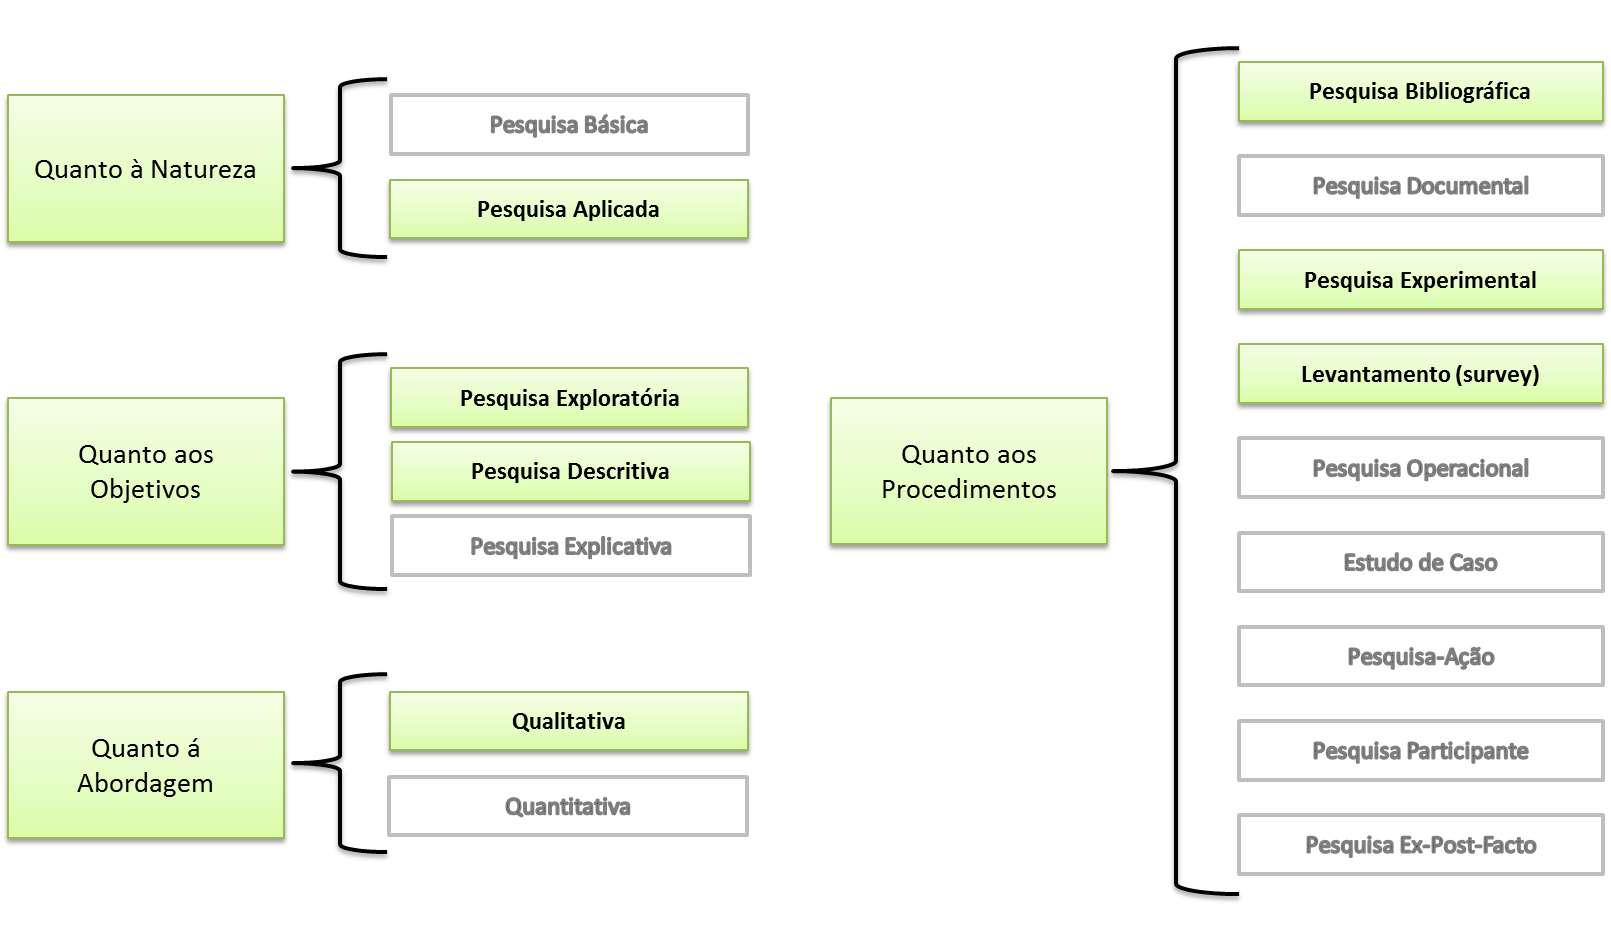
\includegraphics[width=\textwidth]{img/ClassificacaoPesquisa.png}
%	\fonte{Adaptado de \citeonline{Prodanov:2013}.}
%	\label{fig:ClassificacaoPesquisa}
%\end{figure}


\begin{figure}[!htb]
\centering
\caption{Classificação da Pesquisa.}


\tikzset{every picture/.style={line width=0.75pt}} %set default line width to 0.75pt        

\begin{tikzpicture}[x=0.75pt,y=0.75pt,yscale=-1,xscale=1]
%uncomment if require: \path (0,575); %set diagram left start at 0, and has height of 575

%Shape: Rectangle [id:dp4577118281096286] 
\draw  [fill={rgb, 255:red, 80; green, 227; blue, 194 }  ,fill opacity=1 ] (224.94,20) -- (438.21,20) -- (438.21,52.92) -- (224.94,52.92) -- cycle ;
%Rounded Rect [id:dp34276139041627407] 
\draw  [fill={rgb, 255:red, 80; green, 227; blue, 194 }  ,fill opacity=1 ] (117.95,320.19) .. controls (117.95,317.55) and (120.09,315.42) .. (122.73,315.42) -- (237.49,315.42) .. controls (240.13,315.42) and (242.27,317.55) .. (242.27,320.19) -- (242.27,334.51) .. controls (242.27,337.14) and (240.13,339.28) .. (237.49,339.28) -- (122.73,339.28) .. controls (120.09,339.28) and (117.95,337.14) .. (117.95,334.51) -- cycle ;
%Rounded Rect [id:dp8849258160693669] 
\draw  [fill={rgb, 255:red, 80; green, 227; blue, 194 }  ,fill opacity=1 ] (117.95,79.08) .. controls (117.95,76.45) and (120.09,74.31) .. (122.73,74.31) -- (237.49,74.31) .. controls (240.13,74.31) and (242.27,76.45) .. (242.27,79.08) -- (242.27,93.4) .. controls (242.27,96.04) and (240.13,98.17) .. (237.49,98.17) -- (122.73,98.17) .. controls (120.09,98.17) and (117.95,96.04) .. (117.95,93.4) -- cycle ;
%Rounded Rect [id:dp6071364324721369] 
\draw  [fill={rgb, 255:red, 80; green, 227; blue, 194 }  ,fill opacity=1 ] (117.95,182.77) .. controls (117.95,180.13) and (120.09,178) .. (122.73,178) -- (237.49,178) .. controls (240.13,178) and (242.27,180.13) .. (242.27,182.77) -- (242.27,197.09) .. controls (242.27,199.72) and (240.13,201.86) .. (237.49,201.86) -- (122.73,201.86) .. controls (120.09,201.86) and (117.95,199.72) .. (117.95,197.09) -- cycle ;
%Rounded Rect [id:dp4106241999835438] 
\draw  [fill={rgb, 255:red, 80; green, 227; blue, 194 }  ,fill opacity=1 ] (425.68,79.08) .. controls (425.68,76.45) and (427.81,74.31) .. (430.45,74.31) -- (545.22,74.31) .. controls (547.85,74.31) and (549.99,76.45) .. (549.99,79.08) -- (549.99,93.4) .. controls (549.99,96.04) and (547.85,98.17) .. (545.22,98.17) -- (430.45,98.17) .. controls (427.81,98.17) and (425.68,96.04) .. (425.68,93.4) -- cycle ;
%Rounded Same Side Corner Rect [id:dp2840400712193636] 
\draw  [fill={rgb, 255:red, 255; green, 255; blue, 255 }  ,fill opacity=1 ] (141.39,122.24) .. controls (141.39,120.31) and (142.95,118.75) .. (144.88,118.75) -- (277.5,118.75) .. controls (279.42,118.75) and (280.99,120.31) .. (280.99,122.24) -- (280.99,136.19) .. controls (280.99,136.19) and (280.99,136.19) .. (280.99,136.19) -- (141.39,136.19) .. controls (141.39,136.19) and (141.39,136.19) .. (141.39,136.19) -- cycle ;
%Rounded Same Side Corner Rect [id:dp5724415497830746] 
\draw  [fill={rgb, 255:red, 184; green, 233; blue, 134 }  ,fill opacity=1 ] (141.39,154.33) .. controls (141.39,152.4) and (142.95,150.84) .. (144.88,150.84) -- (277.5,150.84) .. controls (279.42,150.84) and (280.99,152.4) .. (280.99,154.33) -- (280.99,168.28) .. controls (280.99,168.28) and (280.99,168.28) .. (280.99,168.28) -- (141.39,168.28) .. controls (141.39,168.28) and (141.39,168.28) .. (141.39,168.28) -- cycle ;
%Rounded Same Side Corner Rect [id:dp14985801223973771] 
\draw  [fill={rgb, 255:red, 184; green, 233; blue, 134 }  ,fill opacity=1 ] (141.39,225.1) .. controls (141.39,223.17) and (142.95,221.61) .. (144.88,221.61) -- (277.5,221.61) .. controls (279.42,221.61) and (280.99,223.17) .. (280.99,225.1) -- (280.99,239.05) .. controls (280.99,239.05) and (280.99,239.05) .. (280.99,239.05) -- (141.39,239.05) .. controls (141.39,239.05) and (141.39,239.05) .. (141.39,239.05) -- cycle ;
%Rounded Same Side Corner Rect [id:dp37387501315114524] 
\draw  [fill={rgb, 255:red, 255; green, 255; blue, 255 }  ,fill opacity=1 ] (141.39,257.19) .. controls (141.39,255.26) and (142.95,253.7) .. (144.88,253.7) -- (277.5,253.7) .. controls (279.42,253.7) and (280.99,255.26) .. (280.99,257.19) -- (280.99,271.15) .. controls (280.99,271.15) and (280.99,271.15) .. (280.99,271.15) -- (141.39,271.15) .. controls (141.39,271.15) and (141.39,271.15) .. (141.39,271.15) -- cycle ;
%Rounded Same Side Corner Rect [id:dp25377701690503685] 
\draw  [fill={rgb, 255:red, 255; green, 255; blue, 255 }  ,fill opacity=1 ] (141.39,289.28) .. controls (141.39,287.36) and (142.95,285.79) .. (144.88,285.79) -- (276.48,285.79) .. controls (278.41,285.79) and (279.97,287.36) .. (279.97,289.28) -- (279.97,303.24) .. controls (279.97,303.24) and (279.97,303.24) .. (279.97,303.24) -- (141.39,303.24) .. controls (141.39,303.24) and (141.39,303.24) .. (141.39,303.24) -- cycle ;
%Rounded Same Side Corner Rect [id:dp13794965074230814] 
\draw  [fill={rgb, 255:red, 184; green, 233; blue, 134 }  ,fill opacity=1 ] (141.39,361.7) .. controls (141.39,359.77) and (142.95,358.21) .. (144.88,358.21) -- (277.5,358.21) .. controls (279.42,358.21) and (280.99,359.77) .. (280.99,361.7) -- (280.99,375.65) .. controls (280.99,375.65) and (280.99,375.65) .. (280.99,375.65) -- (141.39,375.65) .. controls (141.39,375.65) and (141.39,375.65) .. (141.39,375.65) -- cycle ;
%Rounded Same Side Corner Rect [id:dp46839135503439744] 
\draw  [fill={rgb, 255:red, 184; green, 233; blue, 134 }  ,fill opacity=1 ] (141.39,393.79) .. controls (141.39,391.86) and (142.95,390.3) .. (144.88,390.3) -- (277.5,390.3) .. controls (279.42,390.3) and (280.99,391.86) .. (280.99,393.79) -- (280.99,407.75) .. controls (280.99,407.75) and (280.99,407.75) .. (280.99,407.75) -- (141.39,407.75) .. controls (141.39,407.75) and (141.39,407.75) .. (141.39,407.75) -- cycle ;
%Rounded Same Side Corner Rect [id:dp15982706388592272] 
\draw  [fill={rgb, 255:red, 184; green, 233; blue, 134 }  ,fill opacity=1 ] (320.73,121.47) .. controls (320.73,119.51) and (322.31,117.92) .. (324.27,117.92) -- (516.74,117.92) .. controls (518.7,117.92) and (520.29,119.51) .. (520.29,121.47) -- (520.29,135.64) .. controls (520.29,135.64) and (520.29,135.64) .. (520.29,135.64) -- (320.73,135.64) .. controls (320.73,135.64) and (320.73,135.64) .. (320.73,135.64) -- cycle ;
%Rounded Same Side Corner Rect [id:dp7996243350589711] 
\draw  [fill={rgb, 255:red, 255; green, 255; blue, 255 }  ,fill opacity=1 ] (320.73,147.05) .. controls (320.73,145.1) and (322.31,143.51) .. (324.27,143.51) -- (516.74,143.51) .. controls (518.7,143.51) and (520.29,145.1) .. (520.29,147.05) -- (520.29,161.23) .. controls (520.29,161.23) and (520.29,161.23) .. (520.29,161.23) -- (320.73,161.23) .. controls (320.73,161.23) and (320.73,161.23) .. (320.73,161.23) -- cycle ;
%Rounded Same Side Corner Rect [id:dp30014641980293044] 
\draw  [fill={rgb, 255:red, 184; green, 233; blue, 134 }  ,fill opacity=1 ] (320.73,174.64) .. controls (320.73,172.69) and (322.31,171.1) .. (324.27,171.1) -- (516.74,171.1) .. controls (518.7,171.1) and (520.29,172.69) .. (520.29,174.64) -- (520.29,188.81) .. controls (520.29,188.81) and (520.29,188.81) .. (520.29,188.81) -- (320.73,188.81) .. controls (320.73,188.81) and (320.73,188.81) .. (320.73,188.81) -- cycle ;
%Rounded Same Side Corner Rect [id:dp6116193316770886] 
\draw  [fill={rgb, 255:red, 255; green, 255; blue, 255 }  ,fill opacity=1 ] (321.9,203.23) .. controls (321.9,201.27) and (323.48,199.69) .. (325.44,199.69) -- (516.74,199.69) .. controls (518.7,199.69) and (520.29,201.27) .. (520.29,203.23) -- (520.29,217.4) .. controls (520.29,217.4) and (520.29,217.4) .. (520.29,217.4) -- (321.9,217.4) .. controls (321.9,217.4) and (321.9,217.4) .. (321.9,217.4) -- cycle ;
%Rounded Same Side Corner Rect [id:dp9070606782570514] 
\draw  [fill={rgb, 255:red, 255; green, 255; blue, 255 }  ,fill opacity=1 ] (321.9,231.82) .. controls (321.9,229.86) and (323.48,228.27) .. (325.44,228.27) -- (517.33,228.27) .. controls (519.29,228.27) and (520.87,229.86) .. (520.87,231.82) -- (520.87,245.99) .. controls (520.87,245.99) and (520.87,245.99) .. (520.87,245.99) -- (321.9,245.99) .. controls (321.9,245.99) and (321.9,245.99) .. (321.9,245.99) -- cycle ;
%Rounded Same Side Corner Rect [id:dp026422911508531044] 
\draw  [fill={rgb, 255:red, 255; green, 255; blue, 255 }  ,fill opacity=1 ] (321.9,262.41) .. controls (321.9,260.45) and (323.48,258.86) .. (325.44,258.86) -- (517.92,258.86) .. controls (519.87,258.86) and (521.46,260.45) .. (521.46,262.41) -- (521.46,276.58) .. controls (521.46,276.58) and (521.46,276.58) .. (521.46,276.58) -- (321.9,276.58) .. controls (321.9,276.58) and (321.9,276.58) .. (321.9,276.58) -- cycle ;
%Straight Lines [id:da1670575235577536] 
\draw    (577.5,41.4) -- (577.46,86.44) ;


%Straight Lines [id:da8118950691589346] 
\draw    (123.86,339.28) -- (123.86,400.18) ;


%Straight Lines [id:da17291466732826466] 
\draw    (123.86,201.86) -- (124.07,294.85) ;


%Straight Lines [id:da3815361458832034] 
\draw    (123.86,98.17) -- (123.86,159.07) ;


%Straight Lines [id:da3368611079285959] 
\draw    (123.86,128.62) -- (135.85,128.9) ;
\draw [shift={(135.85,128.9)}, rotate = 1.31] [color={rgb, 255:red, 0; green, 0; blue, 0 }  ][line width=0.75]      (5.59,-5.59) .. controls (2.5,-5.59) and (0,-3.09) .. (0,0) .. controls (0,3.09) and (2.5,5.59) .. (5.59,5.59) ;

%Rounded Same Side Corner Rect [id:dp7931997046212467] 
\draw  [fill={rgb, 255:red, 255; green, 255; blue, 255 }  ,fill opacity=1 ] (321.9,292.6) .. controls (321.9,290.64) and (323.48,289.06) .. (325.44,289.06) -- (517.33,289.06) .. controls (519.29,289.06) and (520.87,290.64) .. (520.87,292.6) -- (520.87,306.77) .. controls (520.87,306.77) and (520.87,306.77) .. (520.87,306.77) -- (321.9,306.77) .. controls (321.9,306.77) and (321.9,306.77) .. (321.9,306.77) -- cycle ;
%Rounded Same Side Corner Rect [id:dp28960792030116966] 
\draw  [fill={rgb, 255:red, 255; green, 255; blue, 255 }  ,fill opacity=1 ] (321.9,321.12) .. controls (321.9,319.17) and (323.48,317.58) .. (325.44,317.58) -- (516.74,317.58) .. controls (518.7,317.58) and (520.29,319.17) .. (520.29,321.12) -- (520.29,335.3) .. controls (520.29,335.3) and (520.29,335.3) .. (520.29,335.3) -- (321.9,335.3) .. controls (321.9,335.3) and (321.9,335.3) .. (321.9,335.3) -- cycle ;
%Rounded Same Side Corner Rect [id:dp49389290024820665] 
\draw  [fill={rgb, 255:red, 255; green, 255; blue, 255 }  ,fill opacity=1 ] (321.9,350.65) .. controls (321.9,348.69) and (323.48,347.11) .. (325.44,347.11) -- (517.33,347.11) .. controls (519.29,347.11) and (520.87,348.69) .. (520.87,350.65) -- (520.87,364.82) .. controls (520.87,364.82) and (520.87,364.82) .. (520.87,364.82) -- (321.9,364.82) .. controls (321.9,364.82) and (321.9,364.82) .. (321.9,364.82) -- cycle ;
%Straight Lines [id:da7075016344613365] 
\draw    (224.94,40.57) -- (94.18,40.3) ;


%Straight Lines [id:da8791469913030159] 
\draw    (94.18,40.3) -- (93.5,326.94) ;


%Straight Lines [id:da6200478575277137] 
\draw    (94.42,86.57) -- (117.59,86.65) ;
\draw [shift={(117.59,86.65)}, rotate = 0.2] [color={rgb, 255:red, 0; green, 0; blue, 0 }  ][fill={rgb, 255:red, 0; green, 0; blue, 0 }  ][line width=0.75]      (0, 0) circle [x radius= 3.35, y radius= 3.35]   ;

%Straight Lines [id:da918961853297364] 
\draw    (94.01,190.26) -- (117.95,190.17) ;
\draw [shift={(117.95,190.17)}, rotate = 359.8] [color={rgb, 255:red, 0; green, 0; blue, 0 }  ][fill={rgb, 255:red, 0; green, 0; blue, 0 }  ][line width=0.75]      (0, 0) circle [x radius= 3.35, y radius= 3.35]   ;

%Straight Lines [id:da08443900683214389] 
\draw    (93.5,326.94) -- (118.21,327.19) ;
\draw [shift={(118.21,327.19)}, rotate = 0.57] [color={rgb, 255:red, 0; green, 0; blue, 0 }  ][fill={rgb, 255:red, 0; green, 0; blue, 0 }  ][line width=0.75]      (0, 0) circle [x radius= 3.35, y radius= 3.35]   ;

%Straight Lines [id:da08124554802054562] 
\draw    (577.5,41.4) -- (438.24,41.4) ;


%Straight Lines [id:da8343656632858758] 
\draw    (577.46,86.44) -- (550.6,86.33) ;
\draw [shift={(550.6,86.33)}, rotate = 180.25] [color={rgb, 255:red, 0; green, 0; blue, 0 }  ][fill={rgb, 255:red, 0; green, 0; blue, 0 }  ][line width=0.75]      (0, 0) circle [x radius= 3.35, y radius= 3.35]   ;

%Straight Lines [id:da5805409911126018] 
\draw    (123.86,159.07) -- (135.85,159.34) ;
\draw [shift={(135.85,159.34)}, rotate = 1.31] [color={rgb, 255:red, 0; green, 0; blue, 0 }  ][line width=0.75]      (5.59,-5.59) .. controls (2.5,-5.59) and (0,-3.09) .. (0,0) .. controls (0,3.09) and (2.5,5.59) .. (5.59,5.59) ;

%Straight Lines [id:da08813150434666617] 
\draw    (123.86,230.66) -- (135.85,230.93) ;
\draw [shift={(135.85,230.93)}, rotate = 1.31] [color={rgb, 255:red, 0; green, 0; blue, 0 }  ][line width=0.75]      (5.59,-5.59) .. controls (2.5,-5.59) and (0,-3.09) .. (0,0) .. controls (0,3.09) and (2.5,5.59) .. (5.59,5.59) ;

%Straight Lines [id:da8789308114642371] 
\draw    (123.52,262.48) -- (135.51,262.75) ;
\draw [shift={(135.51,262.75)}, rotate = 1.31] [color={rgb, 255:red, 0; green, 0; blue, 0 }  ][line width=0.75]      (5.59,-5.59) .. controls (2.5,-5.59) and (0,-3.09) .. (0,0) .. controls (0,3.09) and (2.5,5.59) .. (5.59,5.59) ;

%Straight Lines [id:da3029508317300338] 
\draw    (124.07,294.85) -- (136.06,295.12) ;
\draw [shift={(136.06,295.12)}, rotate = 1.31] [color={rgb, 255:red, 0; green, 0; blue, 0 }  ][line width=0.75]      (5.59,-5.59) .. controls (2.5,-5.59) and (0,-3.09) .. (0,0) .. controls (0,3.09) and (2.5,5.59) .. (5.59,5.59) ;

%Straight Lines [id:da18852599605985843] 
\draw    (123.86,400.18) -- (135.85,400.45) ;
\draw [shift={(135.85,400.45)}, rotate = 1.31] [color={rgb, 255:red, 0; green, 0; blue, 0 }  ][line width=0.75]      (5.59,-5.59) .. controls (2.5,-5.59) and (0,-3.09) .. (0,0) .. controls (0,3.09) and (2.5,5.59) .. (5.59,5.59) ;

%Straight Lines [id:da4226131243667748] 
\draw    (123.86,367.26) -- (135.85,367.53) ;
\draw [shift={(135.85,367.53)}, rotate = 1.31] [color={rgb, 255:red, 0; green, 0; blue, 0 }  ][line width=0.75]      (5.59,-5.59) .. controls (2.5,-5.59) and (0,-3.09) .. (0,0) .. controls (0,3.09) and (2.5,5.59) .. (5.59,5.59) ;

%Straight Lines [id:da9099213522511087] 
\draw    (544.28,356.7) -- (526.55,356.59) ;
\draw [shift={(526.55,356.59)}, rotate = 180.35] [color={rgb, 255:red, 0; green, 0; blue, 0 }  ][line width=0.75]      (5.59,-5.59) .. controls (2.5,-5.59) and (0,-3.09) .. (0,0) .. controls (0,3.09) and (2.5,5.59) .. (5.59,5.59) ;

%Straight Lines [id:da6809709538467319] 
\draw    (544.08,98.17) -- (544.28,356.7) ;


%Straight Lines [id:da20079995081938384] 
\draw    (544.28,327.08) -- (526.35,326.97) ;
\draw [shift={(526.35,326.97)}, rotate = 180.35] [color={rgb, 255:red, 0; green, 0; blue, 0 }  ][line width=0.75]      (5.59,-5.59) .. controls (2.5,-5.59) and (0,-3.09) .. (0,0) .. controls (0,3.09) and (2.5,5.59) .. (5.59,5.59) ;

%Straight Lines [id:da3359178127594531] 
\draw    (544.28,299.28) -- (526.55,299.33) ;
\draw [shift={(526.55,299.33)}, rotate = 179.82] [color={rgb, 255:red, 0; green, 0; blue, 0 }  ][line width=0.75]      (5.59,-5.59) .. controls (2.5,-5.59) and (0,-3.09) .. (0,0) .. controls (0,3.09) and (2.5,5.59) .. (5.59,5.59) ;

%Straight Lines [id:da6129689041896622] 
\draw    (544.28,269.01) -- (527.57,269.06) ;
\draw [shift={(527.57,269.06)}, rotate = 179.81] [color={rgb, 255:red, 0; green, 0; blue, 0 }  ][line width=0.75]      (5.59,-5.59) .. controls (2.5,-5.59) and (0,-3.09) .. (0,0) .. controls (0,3.09) and (2.5,5.59) .. (5.59,5.59) ;

%Straight Lines [id:da1529146426955228] 
\draw    (544.28,238.91) -- (526.55,238.64) ;
\draw [shift={(526.55,238.64)}, rotate = 180.89] [color={rgb, 255:red, 0; green, 0; blue, 0 }  ][line width=0.75]      (5.59,-5.59) .. controls (2.5,-5.59) and (0,-3.09) .. (0,0) .. controls (0,3.09) and (2.5,5.59) .. (5.59,5.59) ;

%Straight Lines [id:da8053371107503933] 
\draw    (544.28,210.82) -- (526.17,210.85) ;
\draw [shift={(526.17,210.85)}, rotate = 179.89] [color={rgb, 255:red, 0; green, 0; blue, 0 }  ][line width=0.75]      (5.59,-5.59) .. controls (2.5,-5.59) and (0,-3.09) .. (0,0) .. controls (0,3.09) and (2.5,5.59) .. (5.59,5.59) ;

%Straight Lines [id:da764730117630384] 
\draw    (544.28,181.9) -- (526.43,181.73) ;
\draw [shift={(526.43,181.73)}, rotate = 180.55] [color={rgb, 255:red, 0; green, 0; blue, 0 }  ][line width=0.75]      (5.59,-5.59) .. controls (2.5,-5.59) and (0,-3.09) .. (0,0) .. controls (0,3.09) and (2.5,5.59) .. (5.59,5.59) ;

%Straight Lines [id:da7450524911442942] 
\draw    (544.28,153.99) -- (526.43,153.82) ;
\draw [shift={(526.43,153.82)}, rotate = 180.55] [color={rgb, 255:red, 0; green, 0; blue, 0 }  ][line width=0.75]      (5.59,-5.59) .. controls (2.5,-5.59) and (0,-3.09) .. (0,0) .. controls (0,3.09) and (2.5,5.59) .. (5.59,5.59) ;

%Straight Lines [id:da03969256247317787] 
\draw    (544.28,128.9) -- (526.43,128.72) ;
\draw [shift={(526.43,128.72)}, rotate = 180.55] [color={rgb, 255:red, 0; green, 0; blue, 0 }  ][line width=0.75]      (5.59,-5.59) .. controls (2.5,-5.59) and (0,-3.09) .. (0,0) .. controls (0,3.09) and (2.5,5.59) .. (5.59,5.59) ;


% Text Node
\draw (331.58,36.46) node [scale=1.44] [align=left] {\textbf{Tipo de Pesquisa}};
% Text Node
\draw (180.11,86.24) node  [align=left] {\textbf{Natureza}};
% Text Node
\draw (180.11,189.93) node  [align=left] {\textbf{Objetivo}};
% Text Node
\draw (180.11,327.35) node  [align=left] {\textbf{Abordagem}};
% Text Node
\draw (487.83,86.24) node  [align=left] {\textbf{Procedimento}};
% Text Node
\draw (211.19,127.47) node  [align=left] {Básica};
% Text Node
\draw (211.19,159.56) node  [align=left] {Aplicada};
% Text Node
\draw (211.19,230.33) node  [align=left] {Exploratória};
% Text Node
\draw (211.19,262.42) node  [align=left] {Descritiva};
% Text Node
\draw (210.68,294.52) node  [align=left] {Explicativa};
% Text Node
\draw (211.19,366.93) node  [align=left] {Qualitativa};
% Text Node
\draw (211.19,399.02) node  [align=left] {Quantitativa};
% Text Node
\draw (420.51,126.78) node  [align=left] {Pesquisa Bibliográfica};
% Text Node
\draw (420.51,152.37) node  [align=left] {Pesquisa Documental};
% Text Node
\draw (420.51,179.96) node  [align=left] {Pesquisa Experimental};
% Text Node
\draw (421.09,208.54) node  [align=left] {Levantamento};
% Text Node
\draw (421.38,237.13) node  [align=left] {Pesquisa Operacional};
% Text Node
\draw (421.68,267.72) node  [align=left] {Estudo de Caso};
% Text Node
\draw (421.38,297.91) node  [align=left] {Pesquisa Ação};
% Text Node
\draw (421.09,326.44) node  [align=left] {Pesquisa Participante};
% Text Node
\draw (421.38,355.96) node  [align=left] {Pesquisa Ex-Post-Facto};


\end{tikzpicture}

\fonte{Adaptado de \citeonline{Prodanov:2013}.}
\label{fig:ClassificacaoPesquisa}
\end{figure}

Para \citeonline{Prodanov:2013}, nenhum tipo de pesquisa é autossuficiente, sendo então necessário a mescla de diferentes tipos, tendo um ou outro ponto mais acentuado, para a obtenção de resultados satisfatórios. 
Os métodos escolhidos determinam os procedimentos que devem ser utilizados, tanto na coleta de dados e informações quanto na análise. 

No que se refere a sua natureza, uma pesquisa pode ser básica ou aplicada. 
Este trabalho objetiva desenvolver uma \ac{DSL}, gerando uma ferramenta prática para solucionar algo específico e, sendo assim, pode ser categorizada como uma pesquisa de natureza aplicada.

Do ponto de vista dos seus objetivos, uma pesquisa pode ser classificada como exploratória, descritiva ou explicativa. 
Este estudo se encontra na fase preliminar e tem como finalidade oferecer mais informações sobre o assunto que investiga, logo, é uma pesquisa exploratória em sua fase de concepção. 

A abordagem do problema pode classificar a pesquisa em quantitativa ou qualitativa. 
Este trabalho aplicará conceitos de ambas as categorias.
É previsto que seja realizada uma avaliação preliminar da gramática da \ac{DSL}, onde deverá ocorrer a interpretação dos acontecimentos e a atribuição de significados aos resultados sem requerer necessariamente o uso de métodos e técnicas estatísticas, caracterizando assim essa atividade como uma pesquisa qualitativa. 
Por outro lado, na análise dos resultados da avaliação experimental da solução construída entende-se que será necessário considerar todos os elementos passíveis de serem quantificados, o que significará explicar em números as opiniões e dados para classificar os resultados. Desta forma, será fundamental o uso de recursos e de técnicas estatísticas, definindo assim essa atividade como uma pesquisa quantitativa.

E por fim, com relação a seu procedimentos técnicos, uma pesquisa pode ser categorizada como pesquisa bibliográfica, documental, experimental, levantamento, também chamada de \textit{survey}, pesquisa operacional, estudo de caso, pesquisa \textit{ex-post-facto}, pesquisa-ação e pesquisa participante. 
Este trabalho realiza uma pesquisa bibliográfica nas atividades executadas para o levantamento de sua base teórica e, além disso, também pretende executar uma pesquisa experimental na etapa de avaliação da ferramenta produzida.

%#################################################################
\section{Desenho de Pesquisa} \label{sec:DesenhoPesquisa}
%#################################################################

Para a condução deste estudo foi definido o desenho de pesquisa. 
Nesta atividade, três fases foram determinantes: a fase decisória, a fase construtiva e a fase redacional.

A fase decisória se refere a escolha do tema e a delimitação dos problemas de pesquisa. 
A fase construtiva foi onde ocorreu o planejamento das atividades que devem ser realizadas. 
A fase redacional se refere à escrita do projeto de trabalho e a futura análise de dados que serão colhidos e analisados no andamento do estudo. O desenho de pesquisa foi dividido em duas fases, sendo o \ac{TCC} I apresentado na \autoref{fig:ResearchDesign1} e o \ac{TCC} II na \autoref{fig:ResearchDesign2}.

\begin{figure}[!htb]
	\centering
	\caption{Desenho de pesquisa.}
		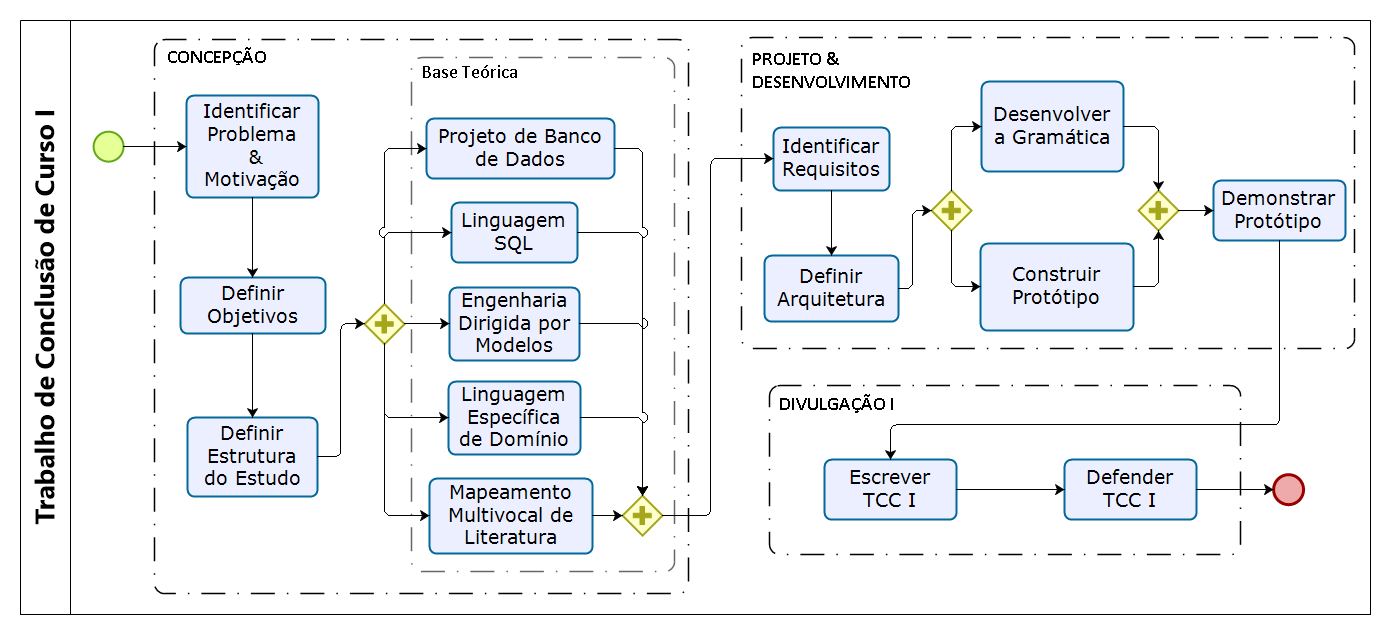
\includegraphics[width=1\textwidth]{img/DesenhoPesquisa1.png}
	\fonte{O autor.}
	\label{fig:ResearchDesign1}
\end{figure}

O projeto foi desenvolvido no \ac{TCC} I, possuindo atividades bem definidas. 
Primeiramente aconteceu o processo de concepção, identificando o problema e a motivação que guiariam todo o estudo. 
Após, foram definidos os objetivos que este trabalho procura atingir. 
Então, houve a elaboração da estrutura geral do estudo em que percebeu-se que era necessário criar uma base teórica bem fundamentada. 
Desta forma, foram caracterizadas as principais áreas que deveriam ser investigadas para o entendimento do domínio do problema. 
Em paralelo, foi realizado um mapeamento multivocal de literatura com o objetivo de encontrar trabalhos similares a esta proposta. 

Com a etapa teórica de concepção realizada, partiu-se então para o projeto inicial da proposta de \ac{DSL}, visando identificar seus requisitos essenciais e sua arquitetura básica. 
Feito isto, deu-se início ao desenvolvimento da descrição de gramática da linguagem e sua implementação de fato. 
Ao fim, um protótipo da ferramenta foi construído. 
A demonstração de uso do protótipo está descrita no Capítulo \autoref{propostaDSL}. 
Como última etapa do \ac{TCC} I, foi realizada a especificação do projeto para a apresentação da proposta.

\begin{figure}[!htb]
	\centering
	\caption{Desenho de pesquisa (continuação).}
		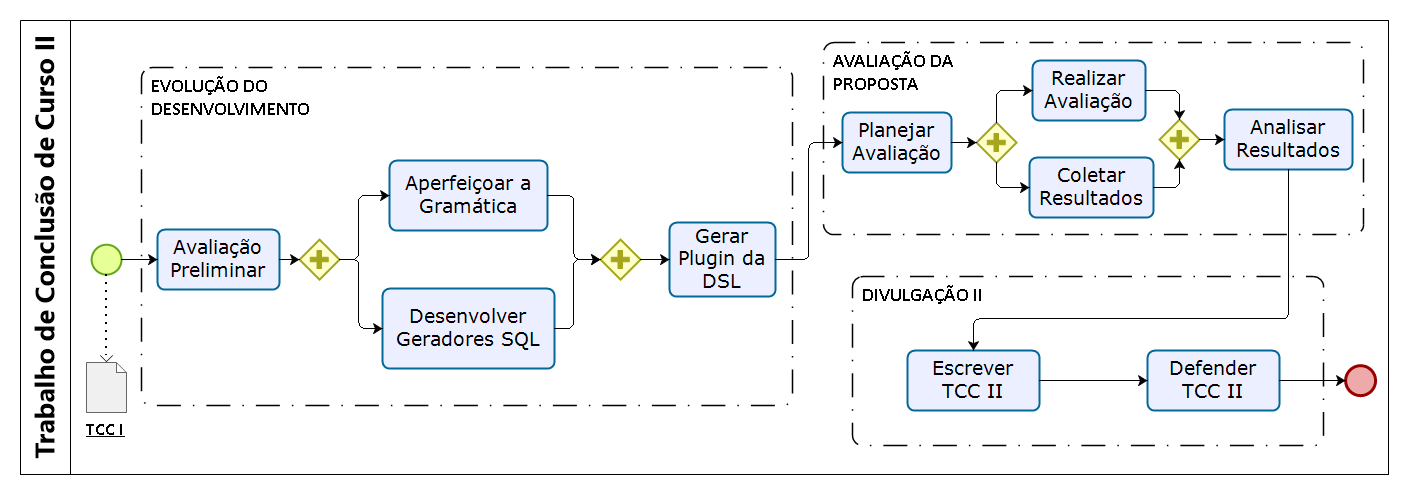
\includegraphics[width=1\textwidth]{img/DesenhoPesquisa2.png}
	\fonte{O autor.}
	\label{fig:ResearchDesign2}
\end{figure}

O \ac{TCC} II tem como entrada os resultados do \ac{TCC} I e inicia-se com uma avaliação preliminar da gramática criada para a \ac{DSL}. 
Após, ocorre a evolução do desenvolvimento, com o aperfeiçoamento da gramática e a construção dos geradores para instruções de Linguagem de Consulta Estruturada, do inglês \ac{SQL}. 
Com essas atividades realizadas, um \textit{plugin} será gerado e incorporado em um \ac{RCP}. 

Com o desenvolvimento finalizado, é desejado que se execute uma avaliação da ferramenta. 
Essa fase vai envolver o planejamento da avaliação para sua realização  e coleta de dados. 
Finalmente, será realizada a análise dos resultados, a escrita do \ac{TCC} II e sua posterior defesa. A \autoref{fig:SinteseTCC} apresenta o resumo geral deste estudo.

% Natureza: 
%     - Pesquisa Aplicada (desenv. procurando gerar uma ferramenta prática para solucionar algo específico)
% Objetivos:
%     - Pesquisa Exploratória (na fase de concepção)
%     - Descritivo (Na fase de avaliação?)
% Procedimentos Técnicos:
%     - Pesquisa Bibliográfica (subfase de base teórica + condução do MSL)
% Abordagem do Problema:
%     - Pesquisa Qualitativa (pela avaliação)

\rowcolors{1}{gray!15}{white}
\begin{table}[!htb]
    \centering
    \caption{Síntese do TCC.}
    \begin{tabular}{m{4.5cm}|m{10cm}}
        \bottomrule
\textbf{Assunto} & Banco de Dados \\
\textbf{Tópico} &  Projeto e Modelagem de Banco de Dados\\
\textbf{Questão de Pesquisa} & Uma \ac{DSL} textual pode auxiliar, em nível conceitual de modelagem, o ensino de projeto e modelagem de banco de dados relacionais? \\
\textbf{Objetivo Principal} & Propor a especificação e realizar a implementação de uma \ac{DSL} para o projeto e modelagem de banco de dados relacionais. \\ 
        \toprule
    \end{tabular}
        \fonte{O autor.}
        \label{fig:SinteseTCC}
\end{table}

%#################################################################
\section{Lições do Capítulo} \label{sec:licMetodo}
%#################################################################


Este capítulo forneceu uma ideia do que é a metodologia de um modo geral e de que forma a pesquisa deste trabalho pode ser classificada. 
Além disso, foi apresentado o desenho estabelecido para a pesquisa, sendo que o que aborda o \ac{TCC} I fornece o entendimento de quais processos foram executados até o momento, e o desenho de \ac{TCC} II aponta o que é  previsto para a sua continuação. 

\chapter{Fundamentação Teórica}\label{fundamentacaoTeorica}

Neste capítulo ocorre a apresentação, de forma abrangente, dos domínios abordados para a realização e compreensão deste trabalho. 
A Seção \ref{sec:ProjetoBD} expõe o que é um projeto de \acp{BD} e suas fases de modelagem para a construção de esquemas de \acp{BD}. 
A Seção \ref{sec:LinguagemSQL} elucida a aplicação da \ac{SQL}, e exemplifica seu uso com alguns exemplos de \acp{SGBD}. 
A Seção \ref{ssec:MDE} aborda a Engenharia Dirigida por Modelos, do inglês \ac{MDE}, e suas aplicações com as \acp{DSL}. 
Na Seção \ref{sec:TrabRelacionados} discute-se os trabalhos relacionados e, por fim, na Seção \ref{sec:LicoesFundamentacaoTeorica} são apresentadas algumas lições aprendidas, bem como os principais tópicos discutidos.

%#################################################################
\section{Projeto de Banco de Dados} \label{sec:ProjetoBD}
%#################################################################

Segundo \citeonline{Date:2004} uma estrutura de \ac{BD} é fundamentalmente um sistema computacional para a manutenção de registros. 
Sistemas desse tipo têm a finalidade de armazenar dados de forma persistente, bem como permitir que usuários definam, busquem e atualizem esses dados para gerar informações pertinentes quando necessário. 
Um \ac{BD} pode ser representado por um modelo de dados, expressado em diferentes níveis e com diferentes técnicas.

Normalmente durante o ciclo de vida do desenvolvimento de software os modelos de dados passam por níveis distintos de transformações. 
Inicialmente não existia um padrão ou recomendação difundida amplamente na indústria, ou mesmo na academia, para o processo de modelagem de dados. 
A estratégia para a utilização de diferentes níveis de projeto e representação tem suas origens com o grupo de estudos em \acp{SGBD} intitulado \textit{ANSI/X3/SPARK}, ainda na década de 1970 \cite{DBLP:1975}.  

Na abordagem proposta, o padrão de definição e especificação de parâmetros e elementos que compreendiam um \ac{BD} levavam em consideração aspectos conceituais, lógicos e físicos. 
Esses aspectos eram chamados genericamente de esquemas (do inglês, \textit{schemas}). 
Esses esquemas na realidade eram fragmentos que serviam, quando em conjunto, para todo o mapeamento da estrutura de um \ac{BD}. 
Esses mesmos conceitos continuam em aplicação até os dias de hoje na implementação de \acp{BD} em \acp{SGBD}.  

De acordo com \citeonline{Cougo:2013}, as dificuldades existentes antes do estabelecimento da arquitetura de três níveis estava essencialmente em um ponto. 
Um mesmo modelo de dados concebido para uma aplicação necessitava de diferentes implementações quando aplicados aos \acp{SGBD} primitivos da época anterior a proposta de três níveis, incluindo modificações significativas no próprio modelo original. 
Isso ocasionava como resultado esquemas bastante particulares e reflexos significativos no modelo de dados final.

Tendo essa realidade como fato, um mesmo modelo de dados gerado para uma única aplicação poderia necessitar de um grande número de diferentes esquemas para abranger as variações de modos de implementação e de visões externas a serem disponibilizadas aos usuários. 
As dificuldades provenientes da administração e manutenção de toda essa variedade de modelos levaram o grupo \textit{ANSI/X3/SPARK} a propor o padrão que tem como ideia central a definição de níveis de esquemas relacionados a um modelo de dados \cite{Cougo:2013}.
Esse padrão acabou por influenciar a proposta de modelagem conceitual de dados concebida por \citeonline{Chen:1976}. 
Sendo assim, os \acp{BD} relacionais até os dias atuais continuam levando em consideração estes conceitos. 

A construção de um \ac{BD} é baseada em um modelo de \ac{BD}, o qual é uma descrição detalhada dos tipos de informações que devem ser armazenadas. 
O projeto de \ac{BD} acontece em três fases distintas de modelagem, onde são gerados o \ac{MCD}, \ac{MLD} e o \ac{MFD} \cite{Heuser:2009}. 
Para a elaboração de modelos de dados deve-se usar uma linguagem de modelagem de dados. 
Existem linguagens gráficas e textuais capazes de descrever os modelos em diferentes níveis de detalhamento e abstração.  

%Entre as vantagens da abordagem de \acp{BD}, \citeonline{Date:2004} enumera as seguintes: (I)Os dados podem ser compartilhados; (II)A redundância de dados pode ser reduzida; (III)A inconsistência pode ser evitada, pelo menos até certo ponto; (IV)O suporte a transações pode ser fornecido; (V)A integridade pode ser mantida; (VI)A segurança pode ser reforçada; (VII)Requisitos podem ser equilibrados; e (VIII)Os padrões podem ser impostos.  

%#################################################################
\subsection{Modelo Conceitual de Dados} \label{ssec:ModelConceitual}
%#################################################################

O \ac{MCD} é a descrição do \ac{BD} de forma independente da implementação utilizada em um \ac{SGBD}. 
Este modelo lista quais dados podem ocorrer no \ac{BD}, mas não registra como estes dados estão armazenados no nível de \ac{SGBD}. 
A técnica mais difundida de \ac{MCD} é a \ac{ER} de \citeonline{Chen:1976}. 
Esta abordagem foi tão bem aceita que passou a ser considerada uma referência definitiva para a modelagem de \acp{BD} relacionais. 
É composta basicamente por um método de diagramação e de conceitos que devem ser respeitados. 
Sendo assim, com esta abordagem os \acp{MCD} são representados com \acp{DER}, como pode ser visto na \autoref{fig:DER}.
    
\begin{figure}[htb]
	\centering
	\caption{Fragmento de DER.}
		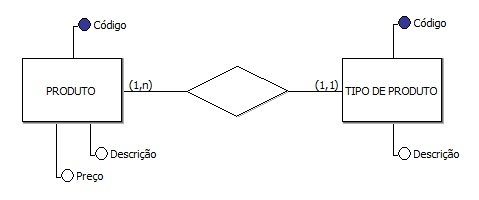
\includegraphics[width=0.6\textwidth]{img/MCD.jpg}
	\fonte{\citeonline{Heuser:2009}.}
	\label{fig:DER}
\end{figure}

%#################################################################
    \subsubsection{Modelo Entidade-Relacionamento} \label{ssec:ModeloER}
%#################################################################

Na abordagem \ac{ER} o conceito principal é o de \textbf{entidade}, o qual é uma representação de um conjunto de objetos do domínio modelado. 
As entidades são simbolizadas por retângulos. 
Contudo, nesta abordagem ainda existem também outros conceitos que são essenciais e devem ser analisados.

Os \textbf{relacionamentos} representam a associação entre os objetos e são sinalizados por losangos. 
A \textbf{cardinalidade} de relacionamentos registra o número de ocorrências com que as entidades podem se associar. 
Existem duas cardinalidades que devem ser atribuídas: a mínima e a máxima. Os \textbf{atributos} são características representadas por pequenos círculos conectados as entidades. 
Na esquerda da \autoref{fig:DER2} é ilustrado um exemplo de \ac{DER} simples e, na direita, uma representação hipotética do conjunto de ocorrências que podem acontecer entre suas entidades. 

\begin{figure}[htb]
	\centering
	\caption{Relacionamentos e cardinalidades.}
		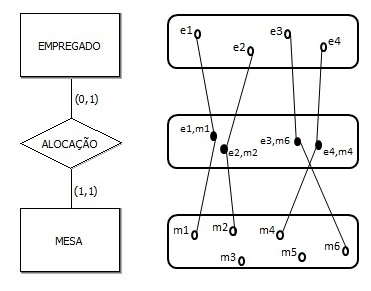
\includegraphics[width=0.5\textwidth]{img/RelCard.jpg}
	\fonte{\citeonline{Heuser:2009}.}
	\label{fig:DER2}
\end{figure}

%#################################################################
\subsubsection{Construtores do Modelo ER} \label{sssec:ModeloER}
%#################################################################

\textcolor{red}{...}

\textcolor{red}{(talvez criar uma tabela sintetizando os construtores, e tirar essa seção e inclui-la na seção anterior)}

\textcolor{red}{Herança}

\textcolor{red}{relacionamentos ternários}

\textcolor{red}{entidades fracas}

\textcolor{red}{atributos}

\textcolor{red}{atributos multivalorados}
    
%#################################################################
\subsubsection{Notações de Modelagem ER} \label{sssec:ModeloER}
%#################################################################
    
\textcolor{red}{ ... }
    
\textcolor{red}{crowsfoot, notação merise, etc...}

%#################################################################
    \subsection{Modelo Lógico de Dados} \label{ssec:ModelLogico}
%#################################################################

Um \ac{MLD} é definido como um modelo que possui a representação dos objetos, relacionamentos e características de acordo com regras de implementação. 
Isso significa que esse modelo tem um nível de abstração do ponto de vista do usuário de um \ac{SGBD}. 
Ainda assim, o modelo lógico é independente do tipo de \ac{SGBD} em que é implementado. 
Na \autoref{fig:MLD} é apresentado um \ac{MLD} gráfico baseado no modelo da \autoref{fig:DER}.

\begin{figure}[htb]
	\centering
	\caption{Exemplo de MLD para BD relacional.}
		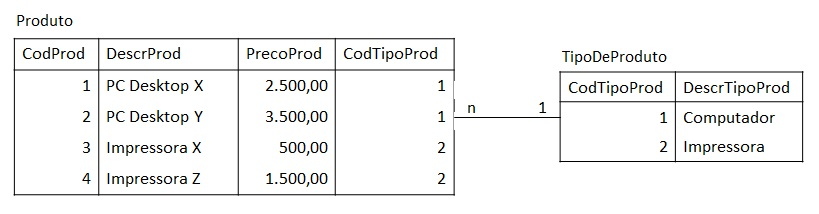
\includegraphics[width=0.8\textwidth]{img/MLD.jpg}
	\fonte{\citeonline{Heuser:2009}.}
	\label{fig:MLD}
\end{figure}

Esse tipo de modelo deve necessariamente respeitar conceitos tais como chaves de acesso, controle de chaves duplicadas, normalização, integridade referencial, controle de redundância de dados, entre outros. 
Este modelo é intrinsecamente relacionado a fase de projeto \cite{Cougo:2013}. 
É importante salientar que essa é uma forma direcionada a um aspecto gráfico, porém existem meios alternativos de se representar estruturalmente o mesmo modelo de forma textual \cite{Martelli:2018}. 
Isso é mostrado na \autoref{fig:LogicoTextual} que apresenta a definição da mesma estrutura descrita na \autoref{fig:MLD}.

\begin{figure}[!htb]
    \caption{Estrutura de um modelo lógico descrita de forma textual.}
    \label{fig:LogicoTextual}
    \centering
    \fbox{
        \parbox{13cm}{
        TipoDeProduto (\underline{CodTipoProd}, DescrTipoProd)\\
        Produto (\underline{CodProd}, DescrProd, PrecoProd, CodTipoProd)\\
        CodTipoProd referencia TipoDeProduto
        }}    
    \fonte{\citeonline{Heuser:2009}.}
\end{figure}

A obtenção de um \ac{MLD} se dá mediante a aplicação de regras de derivação sobre um \ac{MCD} já construído. 
Entretanto, não é raro que desenvolvedores e analistas experientes comecem diretamente pelo processo de modelagem lógica, ignorando a modelagem conceitual. 
Isso ocorre pois esse modelo não se preocupa somente com a representação dos objetos observados no domínio analisado, mas também com outros elementos como chaves, métodos de acesso, formatos de campo, etc. 
Isso implica, em uma última observação, que do ponto de vista formal da definição da abordagem \ac{ER}, esse modelo não se enquadra fielmente como um modelo \ac{ER} \cite{West:2011}.

%#################################################################
    \subsection{\textcolor{red}{Modelo Físico de Dados}} \label{ssec:ModelFisico}
%#################################################################

\textcolor{red}{Um \ac{MFD} caracteriza-se como um modelo em que a representação dos objetos de \ac{BD} já estão em um nível físico de implementação das ocorrências, ou instâncias, das entidades de relacionamentos. 
Cada \ac{SGBD} pode definir diferentes modos de implementação física das características e recursos indispensáveis para o armazenamento e manipulação das estruturas de dados \cite{Cougo:2013}.}

\textcolor{red}{Em geral os modelos físicos apresentam dois aspectos bem representados. 
Primeiramente, existem as ocorrências ou instâncias, seus relacionamentos e a disposição básica dos elementos. 
O outro aspecto diz respeito a alocação nos diversos níveis de agrupamentos possíveis, como as tabelas, linhas (registros), colunas (campos) e blocos \cite{West:2011}.
Em suma é uma sequência lógica de instruções em \ac{SQL}, executadas em um \ac{SGBD}.}

%#################################################################
\section{Linguagem SQL} \label{sec:LinguagemSQL}
%#################################################################

Para a manipulação dos dados a linguagem \ac{SQL} é o  padrão utilizado por sistemas de \acp{BD} relacionais disponíveis no mercado. 
A \ac{SQL} teve sua gênese originalmente nos laboratórios da IBM Research, na década de 1970, com o nome inicial de SEQUEL \cite{Chamberlin:1974}.
A \ac{SQL} é uma linguagem com a versão estável mais recente lançada em 2016 e denominada \texttt{SQL:2016}, possuindo um total de mais de 2000 páginas de especificação\footnote{https://iso.org/standard/63555.html}\footnote{https://standards.iso.org/ittf/PubliclyAvailableStandards/c065143_ISO_IEC_TR_19075-5_2016.zip}\footnote{https://standards.iso.org/ittf/PubliclyAvailableStandards/c067367_ISO_IEC_TR_19075-6_2017.zip}\footnote{https://standards.iso.org/ittf/PubliclyAvailableStandards/c069776_ISO_IEC_TR_19075-7_2017.zip}. 
Entretanto, é importante salientar que ao mesmo tempo em que a maioria dos produtos do mercado trabalham com a \ac{SQL}, estas soluções também deixam de oferecer suporte a determinados aspectos ou ainda os implementa de uma forma diferente da especificação oficial. 

A \ac{SQL} é uma única linguagem, mas comumente é categorizada conforme a funcionalidade das suas instruções. 
A primeira categoria é chamada Linguagem de Definição de Dados, do inglês \ac{DDL}. 
Entre os comandos dessa categoria estão o \texttt{CREATE}, \texttt{ALTER}, \texttt{DROP} e \texttt{TRUNCATE}. 
A segunda categoria é nomeada de Linguagem de Definição de Dados, do inglês \ac{DML}. 
Entre os comandos categorizados como \ac{DML} estão o \texttt{INSERT}, \texttt{UPDATE} e \texttt{DELETE}. 
A terceira categoria é chamada de Linguagem de Consulta de Dados, do inglês \ac{DQL}, a qual possui apenas o comando \texttt{SELECT}. 
A quarta categoria é denominada Linguagem de Transação de Dados, do inglês \ac{DTL}, a qual detém comandos como \texttt{COMMIT} e \texttt{ROLLBACK}.

A \ac{SQL} ainda utiliza uma série de cláusulas (\textit{e.g.} \texttt{FROM}, \texttt{WHERE}, \texttt{GROUP BY}, \texttt{ORDER BY}, \texttt{HAVING}, \texttt{DISTINCT}, \texttt{UNION}), operadores lógicos (\textit{e.g.} \texttt{AND}, \texttt{OR}, \texttt{NOT}), operadores relacionais (\textit{e.g.} \texttt{<}, \texttt{>}, \texttt{<=}, \texttt{>=}, \texttt{=}, \texttt{<>}) e funções de agregação (\textit{e.g.} \texttt{AVG}, \texttt{SUM}, \texttt{COUNT}, \texttt{MAX}, \texttt{MIN}). 
A aplicação destes termos e palavras reservadas, associado a características inspiradas na álgebra relacional, fundamenta a base da \ac{SQL} utilizada pelos \acp{SGBD}.

%#################################################################
    \subsection{Bancos de Dados Relacionais} \label{ssec:SGBDRelacionais}
%#################################################################

Os \acp{SGBD} relacionais suportam o modelo de dados relacional. 
O modelo de dados relacional foi proposto por \citeonline{Codd:1970} e tem como premissa a modelagem orientada a tabelas. 
Um ponto importante a ser citado é o fato de praticamente todos os \acp{SGBD} relacionais do mercado utilizarem \ac{SQL} para a criação e manipulação dos dados.

\begin{figure} [!htb]
    \centering
    \caption{Modelo de dados relacional.}
    \label{fig:ModeloRelacional}
    

\tikzset{every picture/.style={line width=0.75pt}} %set default line width to 0.75pt        

\begin{tikzpicture}[x=0.75pt,y=0.75pt,yscale=-1,xscale=1]
%uncomment if require: \path (0,456.4000015258789); %set diagram left start at 0, and has height of 456.4000015258789

%Shape: Rectangle [id:dp9895438777319416] 
\draw   (199.76,128.06) -- (439.3,128.06) -- (439.3,269.14) -- (199.76,269.14) -- cycle ;
%Straight Lines [id:da9433008870660626] 
\draw    (200.17,183.96) -- (439.3,184.31) ;


%Straight Lines [id:da2966959811071168] 
\draw    (199.96,213.19) -- (439.09,213.54) ;


%Straight Lines [id:da10336227761172356] 
\draw    (199.96,242.26) -- (439.09,242.6) ;


%Shape: Rectangle [id:dp29843450985148356] 
\draw  [fill={rgb, 255:red, 184; green, 233; blue, 134 }  ,fill opacity=1 ] (199.76,128.06) -- (439.07,128.06) -- (439.07,156.8) -- (199.76,156.8) -- cycle ;
%Straight Lines [id:da7072311505307143] 
\draw    (281.21,128) -- (280.87,268.53) ;


%Straight Lines [id:da24303755507006675] 
\draw    (363.25,127.67) -- (362.9,268.19) ;


%Straight Lines [id:da8433947995405431] 
\draw    (84.07,142.75) -- (192.19,143.17) ;
\draw [shift={(194.19,143.18)}, rotate = 180.22] [fill={rgb, 255:red, 0; green, 0; blue, 0 }  ][line width=0.75]  [draw opacity=0] (10.72,-5.15) -- (0,0) -- (10.72,5.15) -- (7.12,0) -- cycle    ;

%Shape: Rectangle [id:dp9829425897866726] 
\draw  [color={rgb, 255:red, 208; green, 2; blue, 27 }  ,draw opacity=1 ] (205.49,217.22) -- (432.44,217.22) -- (432.44,235.51) -- (205.49,235.51) -- cycle ;
%Straight Lines [id:da9003126370670107] 
\draw    (86.49,215.65) -- (157.07,216.08) ;


%Shape: Rectangle [id:dp34368494625131474] 
\draw  [color={rgb, 255:red, 208; green, 2; blue, 27 }  ,draw opacity=1 ] (205.06,188.46) -- (432,188.46) -- (432,206.75) -- (205.06,206.75) -- cycle ;
%Straight Lines [id:da28450929807989755] 
\draw    (157.07,216.08) -- (194.24,201.59) ;
\draw [shift={(196.1,200.87)}, rotate = 518.71] [fill={rgb, 255:red, 0; green, 0; blue, 0 }  ][line width=0.75]  [draw opacity=0] (8.93,-4.29) -- (0,0) -- (8.93,4.29) -- cycle    ;

%Straight Lines [id:da38844388554414944] 
\draw    (157.07,216.08) -- (194.52,227.29) ;
\draw [shift={(196.43,227.87)}, rotate = 196.67000000000002] [fill={rgb, 255:red, 0; green, 0; blue, 0 }  ][line width=0.75]  [draw opacity=0] (8.93,-4.29) -- (0,0) -- (8.93,4.29) -- cycle    ;

%Straight Lines [id:da6694551113867799] 
\draw    (83.2,59.49) -- (298.05,59.09) ;


%Shape: Rectangle [id:dp5574880153243091] 
\draw  [fill={rgb, 255:red, 80; green, 227; blue, 194 }  ,fill opacity=1 ] (199.76,99.32) -- (439.07,99.32) -- (439.07,128.06) -- (199.76,128.06) -- cycle ;
%Straight Lines [id:da8765291155015824] 
\draw    (298.05,59.09) -- (298.06,91.08) ;
\draw [shift={(298.06,93.08)}, rotate = 269.98] [fill={rgb, 255:red, 0; green, 0; blue, 0 }  ][line width=0.75]  [draw opacity=0] (8.93,-4.29) -- (0,0) -- (8.93,4.29) -- cycle    ;

%Shape: Rectangle [id:dp31459180611157866] 
\draw  [color={rgb, 255:red, 208; green, 2; blue, 27 }  ,draw opacity=1 ] (255.94,102.46) -- (381.06,102.46) -- (381.06,124.63) -- (255.94,124.63) -- cycle ;
%Shape: Rectangle [id:dp48382611043878065] 
\draw  [color={rgb, 255:red, 208; green, 2; blue, 27 }  ,draw opacity=1 ] (224.14,134.4) -- (256.9,134.4) -- (256.9,153.28) -- (224.14,153.28) -- cycle ;

% Text Node
\draw (239.74,144.01) node [scale=0.8] [align=left] {A{\scriptsize 1}};
% Text Node
\draw (321.96,144.01) node [scale=0.8] [align=left] {...};
% Text Node
\draw (404.18,144.01) node [scale=0.8] [align=left] {A{\scriptsize n}};
% Text Node
\draw (241.98,168.48) node [scale=1,color={rgb, 255:red, 74; green, 74; blue, 74 }  ,opacity=1 ] [align=left] {{\footnotesize V}{\tiny 1A1}};
% Text Node
\draw (130.91,131.43) node [scale=1] [align=left] {Atributos};
% Text Node
\draw (130.91,151.67) node [scale=1] [align=left] {{\footnotesize (\textbf{colunas})}};
% Text Node
\draw (241.98,196.46) node [scale=1,color={rgb, 255:red, 74; green, 74; blue, 74 }  ,opacity=1 ] [align=left] {{\footnotesize V}{\tiny 2A1}};
% Text Node
\draw (238.98,227.67) node [scale=1,color={rgb, 255:red, 74; green, 74; blue, 74 }  ,opacity=1 ] [align=left] {{\footnotesize V}{\tiny ...}};
% Text Node
\draw (241.98,256.17) node [scale=1,color={rgb, 255:red, 74; green, 74; blue, 74 }  ,opacity=1 ] [align=left] {{\footnotesize V}{\tiny nA1}};
% Text Node
\draw (322.14,168.48) node [scale=1,color={rgb, 255:red, 74; green, 74; blue, 74 }  ,opacity=1 ] [align=left] {{\footnotesize V}{\tiny 1A...}};
% Text Node
\draw (322.14,196.46) node [scale=1,color={rgb, 255:red, 74; green, 74; blue, 74 }  ,opacity=1 ] [align=left] {{\footnotesize V}{\tiny 2A...}};
% Text Node
\draw (317.64,227.67) node [scale=1,color={rgb, 255:red, 74; green, 74; blue, 74 }  ,opacity=1 ] [align=left] {{\footnotesize V}{\tiny ...}};
% Text Node
\draw (322.14,256.17) node [scale=1,color={rgb, 255:red, 74; green, 74; blue, 74 }  ,opacity=1 ] [align=left] {{\footnotesize V}{\tiny nA...}};
% Text Node
\draw (401.22,168.48) node [scale=1,color={rgb, 255:red, 74; green, 74; blue, 74 }  ,opacity=1 ] [align=left] {{\footnotesize V}{\tiny 1An}};
% Text Node
\draw (401.22,196.46) node [scale=1,color={rgb, 255:red, 74; green, 74; blue, 74 }  ,opacity=1 ] [align=left] {{\footnotesize V}{\tiny 2An}};
% Text Node
\draw (398.22,227.67) node [scale=1,color={rgb, 255:red, 74; green, 74; blue, 74 }  ,opacity=1 ] [align=left] {{\footnotesize V}{\tiny ...}};
% Text Node
\draw (401.22,256.17) node [scale=1,color={rgb, 255:red, 74; green, 74; blue, 74 }  ,opacity=1 ] [align=left] {{\footnotesize V}{\tiny nAn}};
% Text Node
\draw (124.43,204.59) node [scale=1] [align=left] {Tuplas};
% Text Node
\draw (124.43,226.56) node [scale=1] [align=left] {{\footnotesize (\textbf{linhas})}};
% Text Node
\draw (180.93,46.33) node [scale=1] [align=left] {Variável de Relação};
% Text Node
\draw (180.93,69.05) node [scale=1] [align=left] {{\footnotesize (\textbf{nome da tabela})}};
% Text Node
\draw (319.41,113.34) node [scale=1] [align=left] {TabelaExemplo};


\end{tikzpicture}

    \fonte{O autor.}
\end{figure}

A \autoref{fig:ModeloRelacional} mostra o esquema estrutural de um modelo relacional. Nele uma tabela, também chamada de entidade, é definida por um nome e um número fixo de atributos com seus tipos de dados indicados. 
Cada tabela deve ter um ou mais atributos identificadores, chamados de chaves, os quais auxiliam a manter a integridade referencial dos dados. 
Um registro, também chamado de ocorrência ou tupla, corresponde a uma linha na tabela e consiste nos valores de cada atributo. 
Uma relação, portanto, consiste em um conjunto de registros associados (referenciados) entre tabelas através das variáveis de relação~\cite{Ramakrishnan:2002}.

% \subsubsection{MySQL}
% O MySQL é um \ac{SGBD} relacional que foi criado por uma empresa sueca chamada MySQL AB, e atualmente é desenvolvido e mantido pela Oracle. 
% O desenvolvimento original do MySQL começou em 1994, mas a primeira versão do MySQL foi lançada apenas em maio de 1995. 
% Foi inicialmente criada para uso pessoal do \ac{SGBD} mSQL baseado na linguagem de baixo nível. 
% O MySQL é usado por muitos aplicativos da \textit{Web} orientados a \ac{BD} como o Drupal, o Joomla, o phpBB e o WordPress.
    
% Entre suas funcionalidades mais relevantes estão o suporte multiplataforma, suporte SSL, \textit{stored procedures}, \textit{triggers}, \textit{views} atualizáveis, \textit{subselects}, entre outras. 
% Atualmente, o MySQL está na versão 8.0, funciona sobre plataformas Windows, Linux, Solaris, macOS e FreeBSD. 
% Existe a versão paga \textit{Enterprise Server} e a versão de código aberto MySQL \textit{Community Server}, gratuita e com licença GPL. 
% É considerado o 2º \ac{SGBD} mais popular~\footnote{https://db-engines.com/en/system/MySQL} entre as opções do mercado pelo portal DB-Engines. 
% Segundo a avaliação publicada em 2019 pela empresa de consultoria Gartner \textit{Group}\footnote{https://gartner.com/reviews/market/operational-dbms}, o MySQL possui uma avaliação de 4,5 de 5 pelo mercado.

% \subsubsection{Microsoft SQL Server}
% O Microsoft SQL Server é um \ac{SGBD} relacional desenvolvido e mantido pela Microsoft. 
% Teve uma versão de teste foi criada em parceria com a Sybase em 1988, mas sua primeira versão para uso comercial foi lançada em abril de 1989. 
% Desde de seu lançamento este \ac{SGBD} sofreu inúmeras melhorias. 
% Atualmente possui diversas versões disponibilizadas no mercado, como a \textit{Enterprise}, a \textit{Standard}, \textit{Web}, \textit{Business Intelligence} e \textit{Workgroup}. 
    
% Também possui uma versão chamada \textit{Express}, uma edição gratuita e reduzida. 
% Essa versão inclui o mecanismo de \ac{BD} principal e, embora não haja limitações quanto ao número de \acp{BD} ou usuários com suporte, ele é limitado ao uso de um processador, 1 GB de memória e 10 GB de arquivos de \ac{BD}. 
% O Microsoft SQL Server pode funcionar sobre plataformas Linux, Microsoft Windows Server e Microsoft Windows.
% Atualmente está na versão SQL Server 2017 e é considerado o 3º \ac{SGBD} mais popular~\footnote{https://db-engines.com/en/system/Microsoft+SQL+Server} no mercado pelo portal DB-Engines. 
% Segundo a avaliação publicada pela Gartner Group, o Microsoft SQL Server possui uma avaliação de 4,4 de 5 pelo mercado em 2019.

% \subsubsection{PostgreSQL}
% O PostgreSQL é um \ac{SGBD} que incorpora o modelo relacional para seus esquemas de dados e suporta a linguagem de consulta padrão \ac{SQL}. 
% Surgiu dentro do projeto do Ingres, outro \ac{SGBD}, na universidade da Califórnia. 
% Lançado em 1996 e mantido atualmente pelo PostgreSQL Global Development Group, é considerado pelo mercado um \ac{SGBD} estável, abrangente e possuidor de boas características de desempenho. 
% É executado em praticamente qualquer plataforma Linux, macOS e Microsoft Windows. 
% O grande diferencial do PostgreSQL para ser um dos \acp{SGBD} de maior sucesso é o fato de ser gratuito e de código aberto por meio da flexível licença BSD.
    
% Entre algumas características suportadas pelo PostgreSQL estão transações, \textit{subselects}, \textit{views}, integridade referencial de chaves estrangeiras, bloqueios sofisticados, tipos definidos pelo usuário, herança, regras variadas, \textit{triggers}, funções, procedimentos armazenáveis, entre outras. 
% Atualmente está na versão 11.3 e é considerado o 4º mais popular~\footnote{https://db-engines.com/en/system/PostgreSQL} entre os \acp{SGBD} existentes pelo portal DB-Engines. 
% Segundo a avaliação publicada pela Gartner Group, o Microsoft SQL Server possui uma avaliação de 4,5 de 5 pelo mercado em 2019.

%#################################################################
\section{\textit{Model-Driven Engineering}} \label{ssec:MDE}
%#################################################################

Conceitualmente um modelo é uma representação, protótipo ou exemplo que se tem por objetivo reproduzir ou imitar de alguma forma. 
A construção de modelos são pontos centrais e importantes em diferentes áreas científicas. 
Na matemática, física e química, por exemplo, o emprego de modelos é tido como vital para a investigação teórica e prática em diferentes campos de estudo \cite{Bailer:2009}.

Em uma análise mais profunda, \citeonline{Brambilla:2017} discutem que, considerando-se a premissa de que um observador e suas observações alteram a própria realidade, é possível se concluir que tudo na percepção de um indivíduo é um modelo, já que absolutamente nada pode ser processado pela mente humana sem ser modelado. 
Em resumo, a criação de modelos é uma tarefa de abstração de domínios e conceitos do mundo real. %\cite{MS:2013}. 
Sendo assim, não é de surpreender que os modelos tenham se tornado cruciais e amplamente adotados também em áreas técnicas como mecânica, engenharia civil e, por fim, na ciência da computação, engenharia da computação e \ac{ES}.

A \ac{MDE}, também chamada de \ac{MDSE}, é uma abordagem da \ac{ES} para desenvolvimento de \textit{software} que tem essencialmente modelos como saídas principais de algum processo. 
Essa abordagem resulta em programas ou atividades de computador executados em \textit{hardware} ou \textit{software} que são gerados automaticamente a partir de modelos \cite{Sommerville:2011}. 
Conceitualmente, a \ac{MDE} fornece apoio a outros conceitos, como o \ac{MDD} e a \ac{MDA}. Na \autoref{fig:MDE_MDD_MDA} a relação entre estes conceitos é ilustrada.

\begin{figure}[!htb]
    \centering
    \caption{Relação de MDE, MDD e MDA.}
    \label{fig:MDE_MDD_MDA}
    

\tikzset{every picture/.style={line width=0.75pt}} %set default line width to 0.75pt        

\begin{tikzpicture}[x=0.75pt,y=0.75pt,yscale=-1,xscale=1]
%uncomment if require: \path (0,300); %set diagram left start at 0, and has height of 300

%Shape: Ellipse [id:dp03875628946363818] 
\draw  [fill={rgb, 255:red, 80; green, 227; blue, 194 }  ,fill opacity=1 ] (91,113.58) .. controls (91,67.97) and (171.7,31) .. (271.25,31) .. controls (370.8,31) and (451.5,67.97) .. (451.5,113.58) .. controls (451.5,159.18) and (370.8,196.15) .. (271.25,196.15) .. controls (171.7,196.15) and (91,159.18) .. (91,113.58) -- cycle ;
%Shape: Ellipse [id:dp565416950765411] 
\draw  [fill={rgb, 255:red, 184; green, 233; blue, 134 }  ,fill opacity=1 ] (136.74,134.53) .. controls (136.74,100.49) and (196.96,72.9) .. (271.25,72.9) .. controls (345.54,72.9) and (405.76,100.49) .. (405.76,134.53) .. controls (405.76,168.56) and (345.54,196.15) .. (271.25,196.15) .. controls (196.96,196.15) and (136.74,168.56) .. (136.74,134.53) -- cycle ;
%Shape: Ellipse [id:dp0635650382067301] 
\draw  [fill={rgb, 255:red, 74; green, 144; blue, 226 }  ,fill opacity=1 ] (179.42,155.65) .. controls (179.42,132.41) and (220.53,113.58) .. (271.25,113.58) .. controls (321.97,113.58) and (363.08,132.41) .. (363.08,155.65) .. controls (363.08,178.88) and (321.97,197.72) .. (271.25,197.72) .. controls (220.53,197.72) and (179.42,178.88) .. (179.42,155.65) -- cycle ;

% Text Node
\draw (190,63) node [scale=1] [align=left] {\textit{\textbf{MDE}}};
% Text Node
\draw (231,96) node [scale=1] [align=left] {\textit{\textbf{MDD}}};
% Text Node
\draw (272.25,136.65) node [scale=1] [align=left] {\textit{\textbf{MDA}}};


\end{tikzpicture}

    \fonte{Adaptado de \citeonline{Ameller:2009}.}
\end{figure}

O \ac{MDD} é um paradigma de desenvolvimento que usa modelos como o principal artefato do processo de desenvolvimento. 
No \ac{MDD} geralmente a implementação é gerada de forma semiautomática a partir dos modelos. 
Apesar de serem vistas como a mesma coisa, o conceito da \ac{MDE} tem origem na \ac{MDA}, proposta em 2001 pelo \ac{OMG}. 
Com diferenças sutis, \citeonline{Sommerville:2011} afirma que a \ac{MDA} concentra-se nos estágios de projeto e implementação do processo de desenvolvimento de software, sendo muito similar ao \ac{MDD}, porém implementando diretrizes específicas da \ac{OMG}. 
Desta forma, conclui-se que a \ac{MDA} é um subconjunto do \ac{MDD}. 
Por outro lado, a \ac{MDE} pode abordar muitos outros tópicos do processo de \ac{ES}, entre eles a engenharia de requisitos baseada em modelos, processos de software para desenvolvimento baseado em modelos, ou ainda, testes baseados em modelos.

A \ac{MDE}, como uma metodologia, auxilia a aplicação das vantagens da modelagem nas atividades de \ac{ES}. 
Para \cite{Brambilla:2017} essa abordagem leva em consideração quatro aspectos fundamentais, listados a seguir.

\begin{enumerate}
  \item \textbf{Conceitos:} os componentes que constroem a metodologia, abrangendo desde artefatos de linguagem até atores, e assim por diante;
  \item \textbf{Notações:} A maneira como os conceitos são representados, ou seja, as linguagens usadas na metodologia;
  \item \textbf{Processos e Regras:} As atividades que levam à elaboração do produto final, as regras para sua administração e controle, e as afirmações sobre as propriedades desejadas (correção, consistência, etc) dos produtos ou do próprio processo;
  \item \textbf{Ferramentas:} Aplicações que facilitam a execução de atividades ou seu controle, abrangendo o processo de produção e apoiando o desenvolvedor no uso das notações.
\end{enumerate}

A motivação por trás da \ac{MDE} é a ideia de se aumentar o nível de abstração do processo de desenvolvimento em geral, para então assim capturar sistemas ou processos como uma coleção de modelos reutilizáveis. 
Logo, ela visa reduzir a dificuldade associada ao desenvolvimento de sistemas de software, em geral mais complexos, por meio do uso de técnicas de modelagem que suportam a separação de interesses e geração automatizada de artefatos de sistemas a partir de modelos \cite{Kleppe:2003}.

De uma forma objetiva, a abordagem \ac{MDA}, ou ainda a \ac{MDD}, é a forma de se realizar a \ac{MDE}. 
Essa abordagem define três camadas que devem ser usadas como pilares para todo o processo, listados a seguir.
A relação conceitual entre esses níveis, com o uso de mecanismos de transformação e regras de transformação, é exemplificado na \autoref{fig:MDALevels}.

\begin{enumerate}
    \item \textbf{\acp{CIM}:} descrevem objetos de negócio e as atividades independentemente de sistemas de suporte;
    \item \textbf{\acp{PIM}:} descrevem como os processos de negócio são suportados por sistemas, vistos como caixas-pretas funcionais, ou seja, desconsiderando as restrições associadas às tecnologias candidatas;
    \item \textbf{\acp{PSM}:} descrevem os componentes do sistema conforme implementados por tecnologias específicas.
\end{enumerate}

\begin{figure}[htb]
	\centering
	\caption{Níveis de abstração do MDA.}
		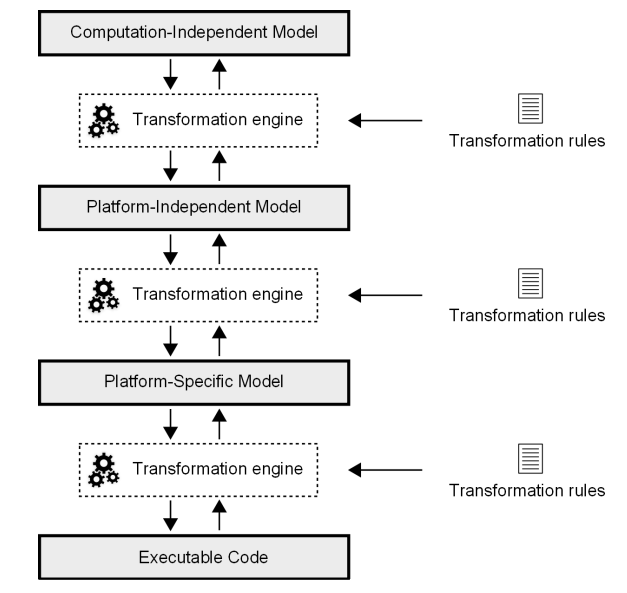
\includegraphics[width=0.57\textwidth]{img/MDA_Process.png}
	\fonte{\citeonline{Frantz:2012}.}
	\label{fig:MDALevels}
\end{figure}

Para melhor esclarecimento, os mecanismos de transformação podem ser entendidos como geradores que tem como entrada a descrição de modelos.
Esses geradores devem processar tais modelos, tendo em si implementados uma série de regras de transformação. 
Por exemplo, no contexto deste estudo um artefato de entrada seria o modelo feito utilizando a \ac{DSL} da proposta, e um mecanismo de transformação seria o gerador do modelo lógico. 
Para tanto, este gerador deve ter descritas ao todas ou parte das regras possíveis de transformação do modelo conceitual para o modelo lógico, ou seja, deve realizar o mapeamento do modelo da \ac{DSL} para um modelo relacional equivalente.
É importante salientar que estes mecanismos de transformação podem estar dispostos em vários níveis. 
Sendo assim, no contexto exemplificado é possível haver até dois (2) mecanismos de transformação: um que faz a transição do modelo conceitual para o lógico e outro que gera código \ac{SQL}.
Este último gerador ainda pode realizar esta tarefa a partir do modelo lógico previamente gerado ou mesmo diretamente do modelo conceitual. 

A separação de interesses da \ac{MDA} baseia-se, por exemplo, na exploração de diferentes \acp{DSL}, cada uma fornecendo construções baseadas em abstrações que são específicas do domínio de um sistema. 
Por conta disto, as \acp{DSL} podem desempenhar um papel de destaque na \ac{MDE} \cite{Schmidt:2006}.


%#################################################################
    \subsection{\textit{Domain-Specific Language}} \label{ssec:DSL}
%#################################################################
    
Para \citeonline{vanDeursen:2000} uma \ac{DSL} é uma linguagem de programação ou linguagem de especificação executável que oferece, por meio de notações e abstrações apropriadas, poder expressivo focado e, geralmente, restrito a um domínio de problema específico. 
Assim como outras linguagens, as \acp{DSL} devem apresentar um conjunto de sentenças bem definidas por uma sintaxe e semântica própria. 
Para \citeonline{Fowler:2010} uma \ac{DSL} é definida como uma linguagem de programação de computadores com expressividade limitada e focada em um domínio particular. 
Entre exemplos conhecidos de \acp{DSL} estão: 

\begin{itemize}
    \item \ac{SQL}, para bancos de dados;
    \item \ac{CSS}, para \textit{layout} de páginas \textit{Web};
    \item \ac{XML}, para codificação de dados;
    \item \ac{UML}, para projeto de software;
    \item \ac{SysML}, para modelagem de sistemas;
    \item \ac{VHDL}, para projeto de hardware;
    \item \LaTeX, para tipografia de documentos.
\end{itemize}
    
Segundo \citeonline{Faveri:2013}, apesar do termo \ac{DSL} poder intuitivamente remeter para um campo de estudos recente, de fato isso não é uma realidade. 
Por exemplo, a APT é uma \ac{DSL} para programação de máquinas controladas numericamente que foi desenvolvida por dois anos a partir de 1957 \cite{Ross:1978}, enquanto o formalismo de especificação de sintaxe \ac{BNF}, o mais usado para notação das linguagens de programação nos dias de hoje, remonta o final da década de 1950 \cite{Backus:1959}.
    
Em razão disso é possível encontrar na literatura muitos estudos que abordam conceitualmente \acp{DSL}, porém com diferentes terminologias.
Entre estas, pode-se citar: \textit{Languages for specialized application} \cite{Sammet:1972}; \textit{Special-purpose languages} \cite{Wexelblat:1978};  \textit{Application Languages} \cite{Martin:1982}; \textit{Task-specific programming languages} \cite{Nardi:1993}; \textit{Specialized languages} \cite{Bergin:1996}. 
    
A aplicação de \acp{DSL} permite que softwares sejam desenvolvidos de forma mais rápida e eficaz. 
A maior vantagem observada no uso de \acp{DSL} é que o conhecimento necessário para a sua aplicabilidade é abstraído para outro nível. 
Desta forma, especialistas do domínio podem entender, validar e modificar o código, adaptando o modelo as suas necessidades, tornando o impacto das mudanças mais fácil de ser compreendido. 
Também existe um aumento significativo na produtividade, confiabilidade, facilidade de uso e flexibilidade \cite{vanDeursen:2000}.

Segundo \citeonline{Mernik:2005} as \acp{DSL} podem ser classificadas sob três dimensões diferentes: \textbf{origem}, \textbf{aparência} e \textbf{implementação}. 
As dimensões de classificação de \ac{DSL} são exibidas na \autoref{fig:ClassDSL}. 
Em relação à origem de uma \ac{DSL}, as opções existentes são as \acp{DSL} \textbf{internas} e \textbf{externas}.

\begin{figure}[!htb]
    \centering
    \caption{Dimensões de uma DSL.}
    

\tikzset{every picture/.style={line width=0.75pt}} %set default line width to 0.75pt        

\begin{tikzpicture}[x=0.75pt,y=0.75pt,yscale=-1,xscale=1]
%uncomment if require: \path (0,408); %set diagram left start at 0, and has height of 408

%Shape: Rectangle [id:dp5982497232353539] 
\draw  [fill={rgb, 255:red, 184; green, 233; blue, 134 }  ,fill opacity=1 ] (43.96,49.84) -- (144.49,49.84) -- (144.49,78.83) -- (43.96,78.83) -- cycle ;
%Shape: Rectangle [id:dp8004700532925917] 
\draw  [fill={rgb, 255:red, 255; green, 255; blue, 255 }  ,fill opacity=1 ] (13.5,154.48) -- (71.89,154.48) -- (71.89,175.74) -- (13.5,175.74) -- cycle ;
%Shape: Rectangle [id:dp6645135942832383] 
\draw  [fill={rgb, 255:red, 184; green, 233; blue, 134 }  ,fill opacity=1 ] (106.92,154.48) -- (165.31,154.48) -- (165.31,175.74) -- (106.92,175.74) -- cycle ;
%Straight Lines [id:da940322594025554] 
\draw [fill={rgb, 255:red, 255; green, 255; blue, 255 }  ,fill opacity=1 ]   (45.99,154.48) -- (72.82,79.88) ;
\draw [shift={(73.5,78)}, rotate = 469.78] [fill={rgb, 255:red, 0; green, 0; blue, 0 }  ][line width=0.75]  [draw opacity=0] (8.93,-4.29) -- (0,0) -- (8.93,4.29) -- cycle    ;

%Straight Lines [id:da03980255509652442] 
\draw [fill={rgb, 255:red, 255; green, 255; blue, 255 }  ,fill opacity=1 ]   (135.35,154.48) -- (106.24,81.86) ;
\draw [shift={(105.5,80)}, rotate = 428.15999999999997] [fill={rgb, 255:red, 0; green, 0; blue, 0 }  ][line width=0.75]  [draw opacity=0] (8.93,-4.29) -- (0,0) -- (8.93,4.29) -- cycle    ;

%Shape: Rectangle [id:dp10111042590582864] 
\draw  [fill={rgb, 255:red, 80; green, 227; blue, 194 }  ,fill opacity=1 ] (192.6,157.7) -- (250.99,157.7) -- (250.99,178.64) -- (192.6,178.64) -- cycle ;
%Straight Lines [id:da05450643799113308] 
\draw [line width=0.75]    (165,165.11) -- (190.7,165.65) ;
\draw [shift={(192.7,165.69)}, rotate = 181.2] [fill={rgb, 255:red, 0; green, 0; blue, 0 }  ][line width=0.75]  [draw opacity=0] (8.93,-4.29) -- (0,0) -- (8.93,4.29) -- cycle    ;

%Shape: Rectangle [id:dp7588912578537257] 
\draw  [fill={rgb, 255:red, 80; green, 227; blue, 194 }  ,fill opacity=1 ] (170.72,50.8) -- (251.62,50.8) -- (251.62,77.86) -- (170.72,77.86) -- cycle ;
%Straight Lines [id:da14516072645219635] 
\draw    (168.39,64.63) -- (144.49,64.33) ;

\draw [shift={(170.38,64.65)}, rotate = 180.71] [fill={rgb, 255:red, 0; green, 0; blue, 0 }  ][line width=0.75]  [draw opacity=0] (8.93,-4.29) -- (0,0) -- (8.93,4.29) -- cycle    ;
%Straight Lines [id:da9230572726153299] 
\draw    (189.85,205.85) -- (210.08,179.33) ;

\draw [shift={(188.64,207.44)}, rotate = 307.34] [color={rgb, 255:red, 0; green, 0; blue, 0 }  ][line width=0.75]    (10.93,-4.9) .. controls (6.95,-2.3) and (3.31,-0.67) .. (0,0) .. controls (3.31,0.67) and (6.95,2.3) .. (10.93,4.9)   ;
%Straight Lines [id:da8579766023100592] 
\draw    (254.77,206.13) -- (235.75,179.06) ;

\draw [shift={(255.92,207.77)}, rotate = 234.92] [color={rgb, 255:red, 0; green, 0; blue, 0 }  ][line width=0.75]    (10.93,-4.9) .. controls (6.95,-2.3) and (3.31,-0.67) .. (0,0) .. controls (3.31,0.67) and (6.95,2.3) .. (10.93,4.9)   ;
%Straight Lines [id:da5652440770199652] 
\draw    (313.68,30.83) -- (251.75,59) ;

\draw [shift={(315.5,30)}, rotate = 155.54] [color={rgb, 255:red, 0; green, 0; blue, 0 }  ][line width=0.75]    (10.93,-4.9) .. controls (6.95,-2.3) and (3.31,-0.67) .. (0,0) .. controls (3.31,0.67) and (6.95,2.3) .. (10.93,4.9)   ;
%Straight Lines [id:da8514029171064224] 
\draw    (312.77,55.31) -- (251.75,65) ;

\draw [shift={(314.75,55)}, rotate = 170.98] [color={rgb, 255:red, 0; green, 0; blue, 0 }  ][line width=0.75]    (10.93,-4.9) .. controls (6.95,-2.3) and (3.31,-0.67) .. (0,0) .. controls (3.31,0.67) and (6.95,2.3) .. (10.93,4.9)   ;
%Shape: Rectangle [id:dp17415476114279294] 
\draw  [fill={rgb, 255:red, 255; green, 255; blue, 255 }  ,fill opacity=1 ] (226.45,207.96) -- (288.15,207.96) -- (288.15,228.89) -- (226.45,228.89) -- cycle ;
%Shape: Rectangle [id:dp5862398976742373] 
\draw  [fill={rgb, 255:red, 255; green, 255; blue, 255 }  ,fill opacity=1 ] (156.18,208.34) -- (217.88,208.34) -- (217.88,229.28) -- (156.18,229.28) -- cycle ;
%Shape: Rectangle [id:dp9794697115134454] 
\draw  [fill={rgb, 255:red, 255; green, 255; blue, 255 }  ,fill opacity=1 ] (315.61,44.77) -- (373.99,44.77) -- (373.99,65.71) -- (315.61,65.71) -- cycle ;
%Shape: Rectangle [id:dp07595309219569546] 
\draw  [fill={rgb, 255:red, 255; green, 255; blue, 255 }  ,fill opacity=1 ] (316.01,18.28) -- (374.4,18.28) -- (374.4,39.21) -- (316.01,39.21) -- cycle ;
%Shape: Rectangle [id:dp9653431753711184] 
\draw  [fill={rgb, 255:red, 80; green, 227; blue, 194 }  ,fill opacity=1 ] (283.98,155.09) -- (376.25,155.09) -- (376.25,176.03) -- (283.98,176.03) -- cycle ;
%Straight Lines [id:da6861278088536416] 
\draw    (269.62,207.98) -- (303.26,178.62) ;
\draw [shift={(304.76,177.3)}, rotate = 498.88] [color={rgb, 255:red, 0; green, 0; blue, 0 }  ][line width=0.75]    (10.93,-4.9) .. controls (6.95,-2.3) and (3.31,-0.67) .. (0,0) .. controls (3.31,0.67) and (6.95,2.3) .. (10.93,4.9)   ;

%Snip Single Corner Rect [id:dp83600176031787] 
\draw  [fill={rgb, 255:red, 255; green, 255; blue, 255 }  ,fill opacity=1 ][dash pattern={on 4.5pt off 4.5pt}] (410.17,129) -- (478.05,129) -- (508.5,159.45) -- (508.5,216) -- (410.17,216) -- cycle ;
%Straight Lines [id:da3854711457144977] 
\draw    (43.9,180.98) -- (43.6,219.23) -- (156.11,219.64) ;

\draw [shift={(43.9,180.98)}, rotate = 270.45] [color={rgb, 255:red, 0; green, 0; blue, 0 }  ][line width=0.75]      (5.59,-5.59) .. controls (2.5,-5.59) and (0,-3.09) .. (0,0) .. controls (0,3.09) and (2.5,5.59) .. (5.59,5.59) ;
%Straight Lines [id:da5105912486039843] 
\draw  [dash pattern={on 0.84pt off 2.51pt}]  (376.25,166.05) -- (409.5,166) ;


%Shape: Rectangle [id:dp1357804439753172] 
\draw  [fill={rgb, 255:red, 255; green, 255; blue, 255 }  ,fill opacity=1 ] (315.01,97.71) -- (373.4,97.71) -- (373.4,118.65) -- (315.01,118.65) -- cycle ;
%Shape: Rectangle [id:dp15166217408811944] 
\draw  [fill={rgb, 255:red, 255; green, 255; blue, 255 }  ,fill opacity=1 ] (315.51,71.28) -- (373.9,71.28) -- (373.9,92.21) -- (315.51,92.21) -- cycle ;
%Straight Lines [id:da2984867724600362] 
\draw    (312.55,82.55) -- (251.62,68.52) ;

\draw [shift={(314.5,83)}, rotate = 192.97] [color={rgb, 255:red, 0; green, 0; blue, 0 }  ][line width=0.75]    (10.93,-4.9) .. controls (6.95,-2.3) and (3.31,-0.67) .. (0,0) .. controls (3.31,0.67) and (6.95,2.3) .. (10.93,4.9)   ;
%Straight Lines [id:da44578022002737083] 
\draw    (312.5,108.03) -- (251.75,74.5) ;

\draw [shift={(314.25,109)}, rotate = 208.9] [color={rgb, 255:red, 0; green, 0; blue, 0 }  ][line width=0.75]    (10.93,-4.9) .. controls (6.95,-2.3) and (3.31,-0.67) .. (0,0) .. controls (3.31,0.67) and (6.95,2.3) .. (10.93,4.9)   ;

% Text Node
\draw (94.23,64.33) node [scale=1] [align=left] {\textbf{Linguagem}};
% Text Node
\draw (42.69,165.11) node [scale=0.8] [align=left] {GPL};
% Text Node
\draw (136.11,165.11) node [scale=0.8] [align=left] {\textbf{DSL}};
% Text Node
\draw (221.79,168.17) node [scale=0.8] [align=left] {Origem};
% Text Node
\draw (257.3,218.42) node [scale=0.8] [align=left] {Externa};
% Text Node
\draw (187.03,218.81) node [scale=0.8] [align=left] {Interna};
% Text Node
\draw (344.8,55.24) node [scale=0.8] [align=left] {Gráfica};
% Text Node
\draw (345.21,28.75) node [scale=0.8] [align=left] {Textual};
% Text Node
\draw (211.17,64.33) node [scale=0.8] [align=left] {Apresentação};
% Text Node
\draw (330.11,165.56) node [scale=0.8] [align=left] {Implementação};
% Text Node
\draw (457.39,176.08) node [scale=0.8] [align=left] {Compilada, \\Interpretada,\\Híbrida, \\Nenhum, \\Etc...};
% Text Node
\draw (344.21,108.18) node [scale=0.8] [align=left] {Simbólica};
% Text Node
\draw (344.71,81.75) node [scale=0.8] [align=left] {Tabular};


\end{tikzpicture}

    \label{fig:ClassDSL}
    \fonte{Adaptado de  \citeonline{Faveri:2013}.}
\end{figure}
    
Uma \ac{DSL} \textbf{interna} é projetada a partir das regras sintáticas e semânticas da gramática de uma linguagem já existente, podendo ser essa uma linguagem de propósito geral, do inglês \ac{GPL}, ou outra \ac{DSL}. 
Sendo assim, para seu funcionamento correto uma \ac{DSL} interna acaba transferindo todas as atividades de verificação léxica, sintática, semântica e de transformação de código ao compilador da linguagem hospedeira.

Uma \ac{DSL} \textbf{externa} é uma linguagem com sintaxe distinta e que depende de uma infraestrutura própria para a análise léxica, sintática, semântica, interpretação, compilação, otimização e geração de código. 
Se comparada a uma \ac{GPL}, uma \ac{DSL} externa possui especificidades similares, porém seus recursos são restritos ao domínio de aplicação para o qual a linguagem é projetada.
    
No que diz respeito à dimensão de \textbf{aparência}, uma \ac{DSL} pode ser classificada como \textbf{textual}, \textbf{gráfica}, \textbf{tabular} e \textbf{simbólica}. 
Quando no formato textual as \acp{DSL} permitem que o domínio seja expressado com caracteres, os quais são então combinados gerando palavras, expressões, sentenças e instruções que seguem as regras gramaticais previamente estabelecidas na linguagem. 
As \acp{DSL} não textuais seguem a mesma lógica, mas utilizando-se de modelos gráficos para permitir que o usuário possa expressar conhecimento de domínio com um maior nível de compreensão e empregando para tal o uso de símbolos, tabelas, figuras e conectores. 
    
E finalmente, no que se refere a dimensão de \textbf{implementação}, as \acp{DSL} podem ser classificadas tendo em vista a perspectiva de sua execução. 
Essas classificações formam quatro grupos: 
(i) \acp{DSL} de execução bem definidas (\textit{e.g.} Excel Macro Language); 
(ii) \acp{DSL} que servem de entrada para geradores de aplicação; 
(iii) \acp{DSL} não executáveis mas úteis como entrada de geradores de aplicação; 
(iv) \acp{DSL} não projetadas para serem executadas.

É prática usual que o principal aspecto levado em consideração para a construção de uma \acp{DSL} deve ser a sua \textbf{origem}, pois cada abordagem apresenta vantagens e desvantagens específicas que são inerentes a cada tipo \cite{Fowler:2010}. 
Apesar das \acp{DSL} externas poderem ter um esforço associado a sua construção muitas vezes maior do que o de uma \ac{DSL} interna, atualmente existem ferramentas que dão grande suporte a construção de \acp{DSL}. 
Estas ferramentas são conhecidas como \acp{LW} e aplicam conceitos de programação orientada a linguagens, fornecendo um nível de abstração maior no que diz respeito as questões complexas de infraestrutura \cite{Fowler:2005}.
    
%#################################################################    
\subsection{\textit{Language Workbenches}} \label{ssec:LW}
%#################################################################

O desenvolvimento de uma \ac{DSL} não é tarefa trivial pois, como são linguagens de programação, possuem uma sintaxe que é, por consequência lógica, definida por uma gramática. 
Desta forma, se faz necessária a utilização de ferramentas que suportem a definição dos conceitos para a nova linguagem \cite{Fowler:2005}.

Os \acp{LW} são ferramentas que fornecem mecanismos de infraestrutura para a implementação de linguagens de programação, tornando assim a criação de linguagens mais acessível \cite{Wachsmuth:2014}. 
Entre os mecanismos fornecidos nesses ambientes está a formatação automática, validação com base nas restrições descritas na gramática, \textit{syntax highlighting}\footnote{Realce de código-fonte com cor, negrito, etc. Serve para indicar sua estrutura sintática.} e \textit{syntax completion}\footnote{Uma função, como em um mecanismo de busca, que fornece uma ou mais opções de palavras reservadas previstas na gramática a partir dos caracteres que um usuário já inseriu.}. 
A seguir são citados alguns dos mais conhecidos \acp{LW} da atualidade:

\begin{itemize}
    \item \textbf{Xtext:} lançado em 2006, o Xtext é um \textit{framework} de código aberto para o desenvolvimento linguagens de programação textuais, com integração com o ambiente de desenvolvimento integrado, do inglês \ac{IDE}, Eclipse. 
    Para especificar uma linguagem, o desenvolvedor descreve uma gramática no Xtext. 
    Essa gramática descreve como um modelo \textit{Ecore} deve ser derivado de uma notação textual. 
    A partir dessa definição, um gerador de código deriva um analisador ANTLR e as classes para o modelo de objetos. 
    O Xtext também tem um gerador Xtend editável, o que dá a capacidade de se gerar código para qualquer outra gramática. 
    O Xtext inclui recursos inerentes ao \ac{IDE} Eclipse como \textit{syntax highlighting}, \textit{code completion}, \textit{static analysis}, \textit{source-code navigation} e outros. 
    Atualmente está na versão 2.18.0.
    
    \item \textbf{Sirius:} lançado em 2007 em um esforço entre as empresas Thales e Obeo, atualmente o \textit{framework} Sirius é um projeto de licença aberta mantido pela Eclipse Foundation, cujo objetivo é permitir a criação de ferramentas de modelagem. 
    Com o Sirius é possível especificar \acp{DSL} visuais e gerar assim a infraestrutura de editores gráficos.
    O Sirius, assim como o Xtext, possui integração com recursos específicos do ambiente Eclipse. Atualmente está na versão 6.2.1.
    
    \item \textbf{JetBrains MPS:} o JetBrains MPS é um sistema desenvolvido pela JetBrains, empresa da República Tcheca, que usa edição projetiva. 
    Essa abordagem permite aos desenvolvedores uma melhor compreensão, o que a diferencia de outros \acp{LW}. 
    Também possui funções comuns de \acp{IDE} integrado a seu ambiente de desenvolvimento. 
    Está atualmente na versão 2019.1.1 sob a licença Apache 2.0.
    
    \item \textbf{MetaEdit+:} o MetaEdit+ é \ac{LW} proprietário desenvolvido pela companhia finlandesa MetaCase para criar e utilizar \acp{DSL}. 
    Possui duas versões nomeadamente \textit{MetaEdit+ Workbench} e \textit{MetaEdit Modeler}. 
    O \textit{Workbench} inclui ferramentas para projetar e usar/testar linguagens de modelagem enquanto o Modeler inclui ferramentas para se utilizar linguagens de modelagem. 
    Normalmente, o \textit{MetaEdit+ Workbench} é usado pelos desenvolvedores que projetam uma \ac{DSL} do domínio para um projeto. 
    Em seguida, essa linguagem de modelagem é usada para desenvolver produtos finais com o apoio do \textit{MetaEdit+ Modeler}. 
    Atualmente está na versão 5.5 SR1.
\end{itemize}

É interessante se observar que as \acp{LW} textuais em particular fornecem poder de abstração suficiente para, por exemplo, especificar \acp{GLC}.

%#################################################################    
\section{Gramáticas Livres de Contexto} \label{ssec:GLC}
%#################################################################

Na matemática, ciência da computação e linguística, uma linguagem formal consiste em palavras cujas letras são retiradas de um alfabeto e são bem formadas de acordo com um conjunto específico de regras. 
Existem diversas abordagens computacionais que tem por objetivo proporcionar que os computadores possam compreender a \ac{LN} falada e/ou escrita por humanos. 
Compreender neste cenário significa, no mínimo, reconhecer o contexto, fazer análise sintática, semântica, léxica e morfológica. 
Esse conjunto de técnicas computacionais compõem uma área denominada \ac{PLN} \cite{Jurafsky:2009}.

Contudo, mesmo com a evolução tecnológica proporcionada pelo esforço de diversos pesquisadores, a comunicação entre homem e máquina através de \ac{LN} continua sendo um desafio. 
Ainda assim, por ser uma área vasta o \ac{PLN} engloba diversos espectros onde as linguagens podem ser classificadas conforme as regras de formação e sua expressividade. 
Neste sentido a figura do filósofo, linguista e escritor norte-americano Noan Chomsky é um expoente, uma vez que ele estabeleceu uma teoria em 1959 que descreve um conjunto de quatro (4) níveis para a classificação de qualquer linguagem. 
A teoria mostra que há quatro (4) classes de gramáticas capazes de gerar diferentes linguagens \cite{Linz:2016}.

Posteriormente o modelo proposto foi refinado por outros pesquisadores, e conta atualmente com versões de até sete (7) níveis. 
Em razão do foco deste estudo ser uma \ac{GLC}, será abordado o nível dois (2) da definição clássica de Chomsky, expressada na Figura \ref{fig:Chomsky}.

\begin{figure}[!htb]
    \centering
    \caption{Representação dos níveis da Hierarquia de Chomsky.}
    \label{fig:Chomsky}
    

\tikzset{every picture/.style={line width=0.75pt}} %set default line width to 0.75pt        

\begin{tikzpicture}[x=0.75pt,y=0.75pt,yscale=-1,xscale=1]
%uncomment if require: \path (0,478.1979217529297); %set diagram left start at 0, and has height of 478.1979217529297

%Shape: Ellipse [id:dp2589253237302658] 
\draw  [fill={rgb, 255:red, 248; green, 231; blue, 28 }  ,fill opacity=0.74 ] (8.59,137.21) .. controls (8.59,77.01) and (125.4,28.21) .. (269.48,28.21) .. controls (413.56,28.21) and (530.36,77.01) .. (530.36,137.21) .. controls (530.36,197.41) and (413.56,246.21) .. (269.48,246.21) .. controls (125.4,246.21) and (8.59,197.41) .. (8.59,137.21) -- cycle ;
%Shape: Ellipse [id:dp694350790161383] 
\draw  [fill={rgb, 255:red, 126; green, 211; blue, 33 }  ,fill opacity=0.71 ] (51.43,152.88) .. controls (51.43,101.34) and (149.05,59.56) .. (269.48,59.56) .. controls (389.91,59.56) and (487.53,101.34) .. (487.53,152.88) .. controls (487.53,204.43) and (389.91,246.21) .. (269.48,246.21) .. controls (149.05,246.21) and (51.43,204.43) .. (51.43,152.88) -- cycle ;
%Shape: Ellipse [id:dp7384199846467594] 
\draw  [fill={rgb, 255:red, 184; green, 233; blue, 134 }  ,fill opacity=1 ] (96.92,172.24) .. controls (96.92,131.39) and (174.18,98.28) .. (269.48,98.28) .. controls (364.78,98.28) and (442.04,131.39) .. (442.04,172.24) .. controls (442.04,213.09) and (364.78,246.21) .. (269.48,246.21) .. controls (174.18,246.21) and (96.92,213.09) .. (96.92,172.24) -- cycle ;
%Shape: Ellipse [id:dp08042679579621703] 
\draw  [fill={rgb, 255:red, 80; green, 227; blue, 194 }  ,fill opacity=0.7 ] (150.42,191.71) .. controls (150.42,161.61) and (203.72,137.21) .. (269.48,137.21) .. controls (335.24,137.21) and (388.54,161.61) .. (388.54,191.71) .. controls (388.54,221.81) and (335.24,246.21) .. (269.48,246.21) .. controls (203.72,246.21) and (150.42,221.81) .. (150.42,191.71) -- cycle ;
%Straight Lines [id:da6929823208677994] 
\draw    (420,48) -- (526.44,50.88) ;
\draw [shift={(526.44,50.88)}, rotate = 181.55] [color={rgb, 255:red, 0; green, 0; blue, 0 }  ][line width=0.75]      (0,0) .. controls (-3.09,0) and (-5.59,2.5) .. (-5.59,5.59) .. controls (-5.59,8.68) and (-3.09,11.18) .. (0,11.18) ;

%Straight Lines [id:da9940150469857363] 
\draw    (429,89) -- (588.44,91.28) ;
\draw [shift={(588.44,91.28)}, rotate = 180.82] [color={rgb, 255:red, 0; green, 0; blue, 0 }  ][line width=0.75]      (0,0) .. controls (-3.09,0) and (-5.59,2.5) .. (-5.59,5.59) .. controls (-5.59,8.68) and (-3.09,11.18) .. (0,11.18) ;

%Straight Lines [id:da8023852859401694] 
\draw    (406,127) -- (607.44,127.88) ;
\draw [shift={(607.44,127.88)}, rotate = 180.25] [color={rgb, 255:red, 0; green, 0; blue, 0 }  ][line width=0.75]      (0,0) .. controls (-3.09,0) and (-5.59,2.5) .. (-5.59,5.59) .. controls (-5.59,8.68) and (-3.09,11.18) .. (0,11.18) ;

%Straight Lines [id:da75358331134597] 
\draw    (375,166) -- (604.84,167.25) ;
\draw [shift={(604.84,167.25)}, rotate = 180.31] [color={rgb, 255:red, 0; green, 0; blue, 0 }  ][line width=0.75]      (0,0) .. controls (-3.09,0) and (-5.59,2.5) .. (-5.59,5.59) .. controls (-5.59,8.68) and (-3.09,11.18) .. (0,11.18) ;


% Text Node
\draw (269.48,48.76) node [scale=1] [align=left] {\textbf{\textit{Gramáticas Irrestritas}}};
% Text Node
\draw (269.48,126.28) node [scale=1] [align=left] {\textbf{\textit{Gramáticas Livres de Contexto}}};
% Text Node
\draw (269.48,88.11) node [scale=1] [align=left] {\textbf{\textit{Gramáticas Sensíveis ao Contexto}}};
% Text Node
\draw (269.48,164.97) node [scale=1] [align=left] {\textbf{\textit{Gramáticas Regulares}}};
% Text Node
\draw (484,40) node  [align=left] {\textbf{NÍVEL 0}};
% Text Node
\draw (546,81) node  [align=left] {\textbf{NÍVEL 1}};
% Text Node
\draw (569,117) node  [align=left] {\textbf{NÍVEL 2}};
% Text Node
\draw (566,157) node  [align=left] {\textbf{NÍVEL 3}};


\end{tikzpicture}

    \fonte{O autor.}
\end{figure}

Nesta hierarquia toda a classe de gramática é um subconjunto da classe do nível imediatamente acima. 
Por exemplo, toda linguagem livre de contexto também é sensível ao contexto, porém a situação inversa não é sempre verdadeira. 
As \acp{GLC} são poderosas o suficiente para descrever a sintaxe da maioria das linguagens de programação utilizadas na atualidade.

Segundo \citeonline{Linz:2016}, as gramáticas consistem de uma coleção de regras de substituição, também chamadas de produções. 
Cada regra aparece como uma linha na gramática, compreendendo um símbolo e uma cadeia separados por uma seta. 
Estas regras descrevem como as cadeias podem ser reconhecidas ou formadas. 
Uma \ac{GLC} é uma gramática formal em que cada regra de produção é da forma $V \rightarrow w$, onde $V$ é um único símbolo não-terminal(variável) e $w$ é uma cadeia de terminais e/ou variáveis, podendo ainda ser também uma cadeia vazia (palavra vazia). 
O termo "livre de contexto" expressa basicamente o fato de que um $V$ não terminal sempre pode ser substituído por $w$, independentemente do contexto em que ocorre.

Demonstrando em um exemplo simples, a linguagem $L=\{a^{n}b^{n}:n \geq 1\}$ define uma estrutura onde todas as cadeias de caracteres são não vazias, de tamanho par e tem a primeira metade preenchida por "a"s e a segunda metade sempre por "b"s. 
Algumas palavras que essa linguagem aceita são $ab$, $aabb$ e $aaabbb$.
Um exemplo de \ac{GLC} que consegue gerá-las é  ${S\to aSb~|~ab}$, contudo é importante salientar que dependendo da linguagem diferentes gramáticas podem gerá-las.

%#################################################################    
\subsection{Formalismo de Backus-Naur} \label{sssec:BNF}
%#################################################################

A primeira representação da gramática de uma linguagem de programação foi apresentada por John Backus, em 1959, para expressar a linguagem 
Algol. Esta notação seguia o mesmo padrão de \acp{GLC} estudado por linguistas como Chomsky, dando origem a notação \ac{BNF} \cite{Edelweiss:2014}.

A notação \ac{BNF} é utilizada para expressar \acp{GLC} e, em geral, é amplamente empregada para a especificação de \acp{GPL}. 
Porém é uma notação que não se restringe apenas as \acp{GPL}, sendo usada também para expressar protocolos de comunicação, formato de dados e outros tipos de linguagens como as específicas de domínio. 
Em geral não é usado em língua natural porque essa notação não é adequada para gramáticas que dependem de contexto.

Na notação \ac{BNF} é simples e muito similar ao modelo utilizado no campo da linguística para definição de \acp{GLC} pois nela: (\textbf{I}) as variáveis são palavras entre os símbolos $\langle$ e $\rangle$ ; (\textbf{II}) as palavras não delimitadas são terminais; (\textbf{III}) a regra geral de produção ${S\to \alpha}$ é representada como ${S ::= \alpha}$, ou ainda, $\langle SNT \rangle ::= \langle \alpha T~|~\alpha T~+~SNT \rangle$. 

Para compreensão, o "\texttt{$::=$}"~ indica "\textit{é definido como}", o \texttt{$|$} indica "\textit{ou}"~ e os colchetes angulares (\texttt{$\langle~\rangle$}) distinguem nomes de regras de sintaxe, chamados de símbolos não terminais (SNT), dos símbolos de terminais (\texttt{$\alpha T$}) que são escritos exatamente como devem ser representados, sendo estes últimos também conhecidos como palavras reservadas. 
Um exemplo da aplicação da notação \ac{BNF} para definir a estrutura de uma mini-linguagem de programação pode ser expressada conforme a Figura \ref{fig:MiniLanguage}.
\definecolor{javared}{rgb}{0.6,0,0} % for strings
\definecolor{javagreen}{rgb}{0.25,0.5,0.35} % comments
\definecolor{javapurple}{rgb}{0.5,0,0.35} % keywords
\definecolor{javadocblue}{rgb}{0.25,0.35,0.75} % javadoc
\definecolor{verde}{rgb}{0.25,0.5,0.35}
\definecolor{jpurple}{rgb}{0.5,0,0.35}
\definecolor{darkgreen}{rgb}{0.0, 0.2, 0.13}


\lstdefinelanguage{Xtext}{
  sensitive = true,
  keywords={},
  keywords=[2]{ERModel, Domain, Attribute, Entity, Relation, RelationSide, DataType, CardinalityType},
  keywords=[3]{grammar, with, generate, Terminals, enum},
  otherkeywords={*, ?, +, *=, ?=, +=, |},
  keywordstyle=\color{black}\bfseries,
  keywordstyle=[2]\color{javadocblue}\bfseries,
  keywordstyle=[3]\color{javapurple}\bfseries,% for example
%   backgroundcolor=\color{cyan!10},
%   numbers=left,
%   stepnumber=1,
  numbersep=8pt,
  showstringspaces=false,
  breaklines=true,
  frame=top,
  comment=[l]{//},
  morecomment=[s]{/*}{*/},
  commentstyle=\color{black}\ttfamily,
  stringstyle=\color{javared}\ttfamily,
  morestring=[b]',
  morestring=[b]"
  }
  
  \lstdefinelanguage{ERDSL}{
  sensitive = true,
  keywords={},
  keywords=[2]{Domain, Entities, Relationships, isIdentifier, isRelatedWith, isA, zero, one, many},
  keywords=[3]{int, money, string, datetime, file},
  otherkeywords={*, ?, +, *=, ?=, +=, |},
  keywordstyle=\color{black}\bfseries,
  keywordstyle=[2]\color{javapurple}\bfseries,
  keywordstyle=[3]\color{javadocblue}\bfseries,% for example
%   backgroundcolor=\color{cyan!10},
%   numbers=left,
%   stepnumber=1,
  captionpos=t,
  numbersep=8pt,
  showstringspaces=false,
  breaklines=true,
  frame=top,
  comment=[l]{//},
  morecomment=[s]{/*}{*/},
  commentstyle=\color{black}\ttfamily,
  stringstyle=\color{javared}\ttfamily,
  morestring=[b]',
  morestring=[b]"
  }
  
  \lstdefinelanguage{BNF}{
  sensitive = true,
  keywords={},
  keywords=[2]{},
  otherkeywords={::= , |, <, >},
  keywordstyle=\color{javapurple}\bfseries,
  keywordstyle=[2]\color{javapurple}\bfseries,
  keywordstyle=[3]\color{javadocblue}\bfseries,% for example
%   backgroundcolor=\color{cyan!10},
%   numbers=left,
%   stepnumber=1,
  captionpos=t,
  numbersep=8pt,
  showstringspaces=false,
  breaklines=true,
  frame=top,
  comment=[l]{//},
  morecomment=[s]{/*}{*/},
  commentstyle=\color{darkgreen}\ttfamily,
  stringstyle=\color{javared}\ttfamily,
  morestring=[b]',
  morestring=[b]"
  }
  
  
  
  

\begin{figure}
    \centering
    \caption{Exemplo de mini-linguagem definida com \ac{BNF}.}
    \label{fig:MiniLanguage}
    \begin{scriptsize}
    \begin{lstlisting}[language = BNF , frame = trbl]
<program> ::= 
            program 
                <declaration_seq>
            begin
                <statements_seq>
            end ;
    \end{lstlisting}
    \end{scriptsize}
\end{figure}

Esse modelo estabelece a estrutura para um programa genérico de forma abstrata, em alto nível. 
Ele consiste de uma regra chamada \texttt{program} que inicia com a palavra-chave \texttt{program} (essa redundância caracteriza a linguagem não ser sensível ao contexto).
Em seguida vem a regra de \texttt{declaration\_seq}, e após a palavra-chave \texttt{begin} e a sequência de instruções definidas na regra \texttt{statements\_seq}.
Finalmente, a a especificação da palavra-chave \texttt{end} seguida de um ponto e vírgula (\texttt{;}). 

%#################################################################
\section{Lições do Capítulo} \label{sec:LicoesFundamentacaoTeorica}
%#################################################################

Os conceitos mais importantes para este trabalho foram apresentados neste capítulo. 
Foi necessário investigar dois grandes domínios, sendo eles: (i) projeto e modelagem de \ac{BD} e (ii) \ac{MDE}. 
Dentre os temas abordados destaca-se a Seção \ref{ssec:DSL}, a qual apresenta definições importantes para a compreensão do que é de fato uma \ac{DSL}, bem como são definidas \acp{GLC} para representá-la. 
A Seção \ref{ssec:LW} também merece destaque pois cita alguns \acp{LW}, dentre eles o Xtext que acabou por ser a ferramenta selecionada para a construção do protótipo da proposta deste estudo.
%#################################################################
\chapter{Mapeamento Multivocal de Literatura}\label{mapeamentoLiteratura}
%#################################################################

Esse capítulo descreve os procedimentos adotados para a investigação da literatura realizada para este estudo. 
Para este propósito ser alcançado foi realizado o planejamento e a execução de um Mapeamento Multivocal da Literatura, do inglês \ac{MLM}. 
Para isto foram aplicadas diretrizes bem estabelecidas conceitualmente por diversos trabalhos \cite{Kitchenham:2007, Petersen:2008, Nakagawa:2017}.  

O protocolo seguido é descrito de forma detalhada na Seção \ref{sec:Protocolo}. 
%Na Subseção \ref{ssec:QPs} são elencadas as nossas \ac{QP}, as fontes de busca na Subseção \ref{ssec:FontesBuscas}. 
%Na Subseção \ref{ssec:StringBusca} apresenta-se os termos e a \textit{string} gerada a partir deles. 
%Os critérios de seleção são categorizados em \acp{CI} e \acp{CE} na Subseção \ref{ssec:CritSelecao}. 
%A avaliação de qualidade feita nos estudos primários é explicada na Subseção \ref{tab:AvalQualidade}. 
%Na Subseção \ref{ssec:EstratExtDados} são especificados os dados que deveriam ser observados nos estudos, caracterizando nossa estratégia de extração de dados. 
Na Seção \ref{sec:ExecMapeamento} é relatado todo o processo de execução do mapeamento multivocal. 
Os resultados provenientes da execução são analisados e discutidos na Seção \ref{sec:ResultDis}. 
As ameaças ao \ac{MLM} são debatidas na Seção \ref{sec:AmeacaVal} e, por fim, são pontuadas algumas lições do capítulo na Seção \ref{sec:LicoesMapeamento}.


%#################################################################
\section{Protocolo} \label{sec:Protocolo}
%#################################################################

Um \ac{MLM} é uma forma de Mapeamento Sistemático de Literatura, do inglês \ac{SLM}, que inclui a literatura cinza. 
Os \acp{MLM} são úteis para pesquisadores e para profissionais pois fornecem visões abrangentes sobre o estado da arte e da prática em uma determinada área. 
Neste estudo conduziu-se um \ac{MLM} utilizando o processo de \ac{SLM} definido por Petersen~\cite{Petersen:2008} e as diretrizes propostas por \citeonline{Garousi:2019} para pesquisa na literatura cinza.

Um \ac{SLM} envolve uma busca para determinar que tipos de estudos abordam as questões de pesquisa que se objetiva investigar, além de possibilitar a classificação e extração de dados que possam gerar informações relevantes~\cite{Bailey:2007}. 
Com o propósito de ter a obtenção de resultados confiáveis e reproduzíveis em um \ac{SLM}, é vital que uma série de atividades bem definidas e estruturadas sejam seguidas \cite{Nakagawa:2017}. 
Na \autoref{fig:SystematicMappingProcess} é apresentado o processo de \ac{SLM} realizado neste estudo, com base na proposição realizada por \citeonline{Petersen:2008}. %Em linhas gerais este processo define todas as etapas necessárias para conduzir o \ac{SLM}. 
%Isso compreende a delimitação das \acp{QP}, a escolha das bases a serem utilizadas, a aplicação dos critérios de seleção, a estratégia de leitura e extração de dados dos estudos, a avaliação de qualidade e a síntese dos resultados obtidos.

\begin{figure}[htb]
	\centering
	\caption{Processo de mapeamento sistemático.}
		%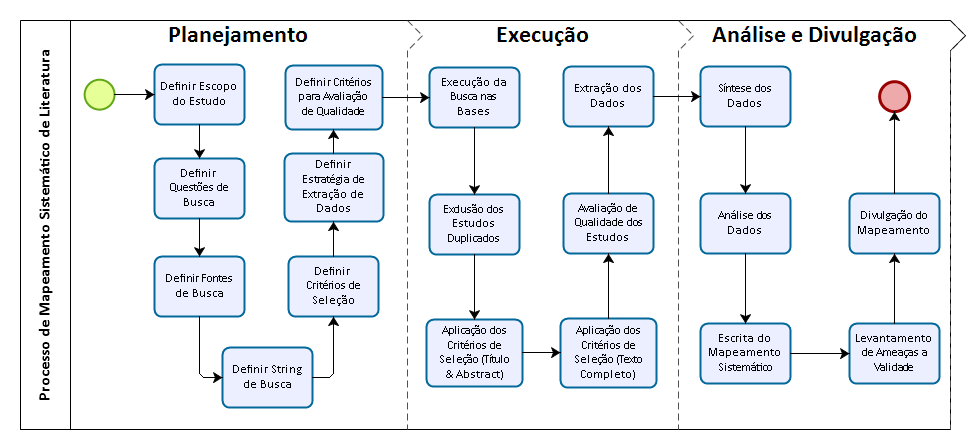
\includegraphics[width=\textwidth]{img/ProcessoMSL.png}
		\tikzset{every picture/.style={line width=0.75pt}} %set default line width to 0.75pt        

\begin{tikzpicture}[x=0.75pt,y=0.75pt,yscale=-1,xscale=1]
%uncomment if require: \path (0,295); %set diagram left start at 0, and has height of 295

%Pentagon Arrow [id:dp6278377926239387] 
\draw   (53.7,53) -- (161.5,53) -- (185.5,76.13) -- (161.5,99.25) -- (53.7,99.25) -- cycle ;
%Chevron Arrow [id:dp8061814950023936] 
\draw   (169.99,53) -- (274.76,53) -- (299.27,76.13) -- (274.76,99.25) -- (169.99,99.25) -- (194.5,76.13) -- cycle ;
%Chevron Arrow [id:dp5292331748785577] 
\draw   (283.07,53) -- (387.84,53) -- (412.35,76.13) -- (387.84,99.25) -- (283.07,99.25) -- (307.58,76.13) -- cycle ;
%Chevron Arrow [id:dp23027191263172608] 
\draw   (509.23,53) -- (618.86,53) -- (644.5,76.13) -- (618.86,99.25) -- (509.23,99.25) -- (534.87,76.13) -- cycle ;
%Chevron Arrow [id:dp12330558695774196] 
\draw   (396.15,53) -- (500.92,53) -- (525.42,76.13) -- (500.92,99.25) -- (396.15,99.25) -- (420.65,76.13) -- cycle ;
%Rounded Rect [id:dp4602302829049887] 
\draw   (61.27,138.93) .. controls (61.27,135.47) and (64.08,132.67) .. (67.54,132.67) -- (148.65,132.67) .. controls (152.11,132.67) and (154.91,135.47) .. (154.91,138.93) -- (154.91,157.73) .. controls (154.91,161.19) and (152.11,164) .. (148.65,164) -- (67.54,164) .. controls (64.08,164) and (61.27,161.19) .. (61.27,157.73) -- cycle ;
%Rounded Rect [id:dp8032081633216976] 
\draw   (523.69,138.93) .. controls (523.69,135.47) and (526.5,132.67) .. (529.96,132.67) -- (611.07,132.67) .. controls (614.53,132.67) and (617.33,135.47) .. (617.33,138.93) -- (617.33,157.73) .. controls (617.33,161.19) and (614.53,164) .. (611.07,164) -- (529.96,164) .. controls (526.5,164) and (523.69,161.19) .. (523.69,157.73) -- cycle ;
%Rounded Rect [id:dp3313220993143424] 
\draw   (408.8,138.93) .. controls (408.8,135.47) and (411.6,132.67) .. (415.06,132.67) -- (496.17,132.67) .. controls (499.63,132.67) and (502.44,135.47) .. (502.44,138.93) -- (502.44,157.73) .. controls (502.44,161.19) and (499.63,164) .. (496.17,164) -- (415.06,164) .. controls (411.6,164) and (408.8,161.19) .. (408.8,157.73) -- cycle ;
%Rounded Rect [id:dp4120899111688079] 
\draw   (293.04,138.57) .. controls (293.04,135.11) and (295.84,132.3) .. (299.3,132.3) -- (380.41,132.3) .. controls (383.87,132.3) and (386.68,135.11) .. (386.68,138.57) -- (386.68,157.37) .. controls (386.68,160.83) and (383.87,163.64) .. (380.41,163.64) -- (299.3,163.64) .. controls (295.84,163.64) and (293.04,160.83) .. (293.04,157.37) -- cycle ;
%Rounded Rect [id:dp45930303754942536] 
\draw   (177.13,138.93) .. controls (177.13,135.47) and (179.94,132.67) .. (183.4,132.67) -- (264.5,132.67) .. controls (267.97,132.67) and (270.77,135.47) .. (270.77,138.93) -- (270.77,157.73) .. controls (270.77,161.19) and (267.97,164) .. (264.5,164) -- (183.4,164) .. controls (179.94,164) and (177.13,161.19) .. (177.13,157.73) -- cycle ;
%Down Arrow [id:dp3807248413929003] 
\draw  [line width=0.75]  (90.13,118.6) -- (100.42,118.6) -- (100.42,99.1) -- (121,99.1) -- (121,118.6) -- (131.3,118.6) -- (110.71,131.6) -- cycle ;
%Down Arrow [id:dp47792969981808375] 
\draw  [line width=0.75]  (204.34,118.6) -- (214.63,118.6) -- (214.63,99.1) -- (235.21,99.1) -- (235.21,118.6) -- (245.5,118.6) -- (224.92,131.6) -- cycle ;
%Down Arrow [id:dp6527476506757643] 
\draw  [line width=0.75]  (320.47,118.6) -- (330.76,118.6) -- (330.76,99.1) -- (351.34,99.1) -- (351.34,118.6) -- (361.63,118.6) -- (341.05,131.6) -- cycle ;
%Down Arrow [id:dp6109879640313591] 
\draw  [line width=0.75]  (434.68,118.6) -- (444.97,118.6) -- (444.97,99.1) -- (465.55,99.1) -- (465.55,118.6) -- (475.84,118.6) -- (455.26,131.6) -- cycle ;
%Down Arrow [id:dp08052269206416462] 
\draw  [line width=0.75]  (548.88,118.6) -- (559.17,118.6) -- (559.17,99.1) -- (579.75,99.1) -- (579.75,118.6) -- (590.04,118.6) -- (569.46,131.6) -- cycle ;
%Straight Lines [id:da6425776226592788] 
\draw [line width=1.5]  [dash pattern={on 1.69pt off 2.76pt}]  (148.07,132) -- (183.21,102.37) ;
\draw [shift={(185.5,100.43)}, rotate = 499.86] [fill={rgb, 255:red, 0; green, 0; blue, 0 }  ][line width=1.5]  [draw opacity=0] (11.61,-5.58) -- (0,0) -- (11.61,5.58) -- cycle    ;

%Straight Lines [id:da624041708353656] 
\draw [line width=1.5]  [dash pattern={on 1.69pt off 2.76pt}]  (264.75,132) -- (299.89,102.37) ;
\draw [shift={(302.18,100.43)}, rotate = 499.86] [fill={rgb, 255:red, 0; green, 0; blue, 0 }  ][line width=1.5]  [draw opacity=0] (11.61,-5.58) -- (0,0) -- (11.61,5.58) -- cycle    ;

%Straight Lines [id:da30892482975542945] 
\draw [line width=1.5]  [dash pattern={on 1.69pt off 2.76pt}]  (380.65,131.73) -- (415.79,102.1) ;
\draw [shift={(418.09,100.16)}, rotate = 499.86] [fill={rgb, 255:red, 0; green, 0; blue, 0 }  ][line width=1.5]  [draw opacity=0] (11.61,-5.58) -- (0,0) -- (11.61,5.58) -- cycle    ;

%Straight Lines [id:da19825567767990848] 
\draw [line width=1.5]  [dash pattern={on 1.69pt off 2.76pt}]  (496.41,132) -- (531.56,102.37) ;
\draw [shift={(533.85,100.43)}, rotate = 499.86] [fill={rgb, 255:red, 0; green, 0; blue, 0 }  ][line width=1.5]  [draw opacity=0] (11.61,-5.58) -- (0,0) -- (11.61,5.58) -- cycle    ;


% Text Node
\draw (111.66,60.53) node [scale=0.7] [align=left] {Definir};
% Text Node
\draw (112.75,74.83) node [scale=0.7] [align=left] {Questões};
% Text Node
\draw (111.66,88.6) node [scale=0.7] [align=left] {de Pesquisa};
% Text Node
\draw (234.55,68.76) node [scale=0.7] [align=left] {Conduzir};
% Text Node
\draw (235.84,82.37) node [scale=0.7] [align=left] {Busca};
% Text Node
\draw (347.88,68.76) node [scale=0.7] [align=left] {Triagem};
% Text Node
\draw (348.71,81.64) node [scale=0.7] [align=left] {dos Estudos};
% Text Node
\draw (463.25,62.65) node [scale=0.7] [align=left] {Busca de};
% Text Node
\draw (465.75,75.78) node [scale=0.7] [align=left] {Palavras-Chave};
% Text Node
\draw (462.75,89.1) node [scale=0.7] [align=left] {no Resumo};
% Text Node
\draw (573.99,63) node [scale=0.7] [align=left] {Extração dos Dados};
% Text Node
\draw (571.87,75.27) node [scale=0.7] [align=left] {e Processo};
% Text Node
\draw (569.37,89.19) node [scale=0.7] [align=left] {de Mapeamento};
% Text Node
\draw (110.09,142.14) node [scale=0.7] [align=left] {Definição do};
% Text Node
\draw (108.31,155.98) node [scale=0.7] [align=left] {Escopo};
% Text Node
\draw (572.51,142.14) node [scale=0.7] [align=left] {Mapeamento};
% Text Node
\draw (570.74,155.98) node [scale=0.7] [align=left] {Sistemático};
% Text Node
\draw (457.62,142.14) node [scale=0.7] [align=left] {Classificação};
% Text Node
\draw (455.84,155.98) node [scale=0.7] [align=left] {dos Estudos};
% Text Node
\draw (341.85,141.77) node [scale=0.7] [align=left] {Estudos};
% Text Node
\draw (340.08,155.62) node [scale=0.7] [align=left] {Relevantes};
% Text Node
\draw (225.95,142.14) node [scale=0.7] [align=left] {Todos os};
% Text Node
\draw (224.17,155.98) node [scale=0.7] [align=left] {Estudos};


\end{tikzpicture}
	\fonte{Adaptado de \citeonline{Petersen:2008}.}
	\label{fig:SystematicMappingProcess}
\end{figure}

%#################################################################
    \subsection{Questões de Pesquisa} \label{ssec:QPs}
%#################################################################

Levando-se em consideração o objetivo geral deste trabalho, o qual é desenvolver uma \ac{DSL} para a modelagem conceitual de \acp{BD}, foram formulados os seguintes questionamentos que serviram de guia para o restante do \ac{MLM}:

\begin{itemize}
    \small
    \item \textbf{QP1.}: Qual o estado da arte do desenvolvimento de DSLs para transformação de modelos em ER?
    \item \textbf{QP1.1.}: Quais são as metodologias, técnicas e propostas de refinamento (desenho automatizado) baseado em modelos de dados?
    \item \textbf{QP1.2.}: Qual é o ferramental utilizado como apoio ao desenvolvimento dessas DSL?
    \item \textbf{QP1.3.}: Quais são as representações de objetos de \ac{BD} adotadas ou sugeridas nas DSL propostas?
    \item \textbf{QP2} Quais os métodos de avaliação utilizados nos estudos?
    \item \textbf{QP2.1.}: Quais os pontos positivos e negativos observados na execução dos estudos?
    \item \textbf{QP2.2.}: Quais desafios são apontados após execução dos estudos empíricos?
    \item \textbf{QP3.}: Quais são as ferramentas para modelagem conceitual de \acp{BD}? 
    \item \textbf{QP3.1.}: Quais são as notações que estas ferramentas usam?
    \item \textbf{QP3.2.}: Quais são os níveis de modelagem de \ac{BD} (Conceitual, Lógico, Físico) que estas ferramentas suportam?
\end{itemize}

%#################################################################
    \subsection{Fontes de Busca} \label{ssec:FontesBuscas}
%#################################################################

As bibliotecas digitais são a principal fonte de busca em um \ac{SLM} \cite{Petersen:2008}. 
Para a escolha das fontes de busca desse \ac{SLM} são considerados três requisitos obrigatórios que as bases devem contemplar: 
\textbf{(I)} possuir mecanismo de pesquisa baseado na \textit{Web}; 
\textbf{(II)} ser capaz de usar palavras-chave durante a pesquisa, e;
\textbf{(III)} abranger estudos primários da grande área da Ciência da Computação. 
Na \autoref{tab:BasesDePesquisa} são listadas as bibliotecas digitais selecionadas para este \ac{SLM}.
        
\rowcolors{1}{gray!15}{white}
\begin{table}[!ht]
    \centering
    \footnotesize
    \caption{Bibliotecas digitais utilizadas.}
    \label{tab:BasesDePesquisa}
    \begin{tabular}{m{4cm}m{4cm}m{4cm}}
    \bottomrule
    \rowcolor[HTML]{C0C0C0}
    \textbf{Fonte} & \textbf{Endereço} & \textbf{Tipo} \\ 
    \hline
    ACM Digital library & \textit{dl.acm.org}           & Híbrida\\
    IEEE Xplore         & \textit{ieeexplore.ieee.org}  & Base Bibliográfica \\ 
    ScienceDirect       & \textit{sciencedirect.com}    & Base Bibliográfica \\
    Scopus       & \textit{scopus.com}   & Motor de Busca \\
    SpringerLink        & \textit{link.springer.com}    & Base Bibliográfica \\ 
    \bottomrule
    \end{tabular}
    \fonte{Adaptado de \citeonline{Nakagawa:2017}.}
\end{table}
            
%#################################################################
    \subsection{String de Busca} \label{ssec:StringBusca}
%#################################################################

A elaboração da \textit{string} de busca não é uma tarefa trivial. 
A identificação de uma combinação de termos que permitam encontrar o maior número de estudos primários relevantes de forma objetiva necessita, na maioria dos casos, de experiência e profundo conhecimento sobre a área de pesquisa abordada.  

\rowcolors{1}{gray!15}{white}
\begin{table}[!h]
    \centering
    \small
    \caption{Termos e sinônimos utilizados.}
    \label{tab:DefinicaoSearch}
    \begin{tabular}{m{4.5cm}m{10.5cm}}
        \bottomrule
        \rowcolor[HTML]{C0C0C0}
        \textbf{Termos} & \textbf{Sinônimos}\\
        \hline
        Domain Specific Language & DSL, Domain-Specific Language, Domain-Specific-Language, DSLM, Domain Specific Modeling Language, Domain-Specific Modeling Language, Domain-Specific-Modeling-Language, Query Language \\
        \hline
        Entity-Relationship & ER, Enhanced Entity-Relationship, EER, Database \\
        \toprule
    \end{tabular}
    \fonte{O autor.}
\end{table}
        
Para a formação da \textit{string} de busca é fundamental definir um conjunto de palavras referentes ao tema de pesquisa, bem como os sinônimos considerados expressivos. 
Estes termos devem representar de forma abrangente o tema central do estudo. 
Para este trabalho foram estabelecidos os termos e sinônimos da \autoref{tab:DefinicaoSearch}, sendo que sua combinação gerou a \textit{string} genérica da \autoref{fig:StringBusca}.
        
\begin{figure}[htb]
    \caption{String genérica de busca.}
    \centering
    \small
    \fbox{
    \parbox{14cm}{
    \centering
    \small\texttt{
    (DSL OR Domain Specific Language OR Domain-Specific Language OR Domain-Specific-Language OR DSLM OR Domain Specific Modeling Language OR Domain-Specific Modeling Language OR Domain-Specific-Modeling-Language OR Query Language)
    AND 
    (ER OR Entity-Relationship OR Enhanced Entity-Relationship OR Extended Entity-Relationship OR Database)
    }}}
    \fonte{O autor.}
    \label{fig:StringBusca}
\end{figure}
        
%#################################################################
    \subsection{Critérios de Seleção} \label{ssec:CritSelecao}
%#################################################################
    
Segundo \citeonline{Kitchenham:2007}, os \acp{CI} indicam por qual ou quais parâmetros um estudo é incluído no \ac{SLM}, ou seja, considerado relevante. 
Da mesma forma, os \acp{CE} indicam por qual ou quais parâmetros um estudo é excluído, ou seja, considerado não relevante na pesquisa realizada. 
Para o este trabalho foram determinados os critérios de seleção listados a seguir.


\begin{itemize}
    \item \textbf{Critérios de Inclusão (\ac{CI})}
    \begin{itemize}
        \item CI1: Estudo que propõe alguma técnica, método, abordagem ou ferramenta para a representação e transformação de modelos de \ac{BD} utilizando \acp{DSL}.
    \end{itemize}
\end{itemize}

\begin{itemize}
    \item \textbf{Critérios de Exclusão (\ac{CE})}
    \begin{itemize}
        \item CE1: Estudo com menos de 4 páginas;  
        \item CE2: Estudo que não esteja escrito em inglês;
        \item CE3: Estudo duplicado;
        \item CE4: Estudo que não fornece acesso completo ao seu conteúdo;
        \item CE5: Estudo que não atende o CI1.
    \end{itemize}
\end{itemize}
    
%#################################################################
    \subsection{Avaliação de Qualidade} \label{scec:AvalQualidade}
%#################################################################

Segundo \citeonline{Nakagawa:2017}, embora exemplos de formulários de avaliação de qualidade possam ser encontrados com certa facilidade na literatura, para a elaboração de critérios e definição de seus pesos os pesquisadores envolvidos em cada revisão ou mapeamento devem levar em consideração as particularidades conforme o tema e as questões de pesquisa.
Portanto, em pesquisas desse tipo existe total liberdade para definição o número de \acs{CQ} e seus pesos relacionados. 

Foram definidos sete (7) \acp{CQ} para a avaliação dos estudos primários aprovados após a aplicação dos critérios de seleção. 
Os \acp{CQ} visam quantificar a relevância para que seja possível realizar uma comparação entre os estudos selecionados. 
Foi definido também uma pontuação para ser atribuída a partir das \acp{CQ}. 
Para a definição das pontuações foram estabelecidas siglas para representar a pontuação dos \acp{CQ}. 

\begin{itemize}
    \item \textbf{T: Total}, contemplando de forma integral o critério de qualidade avaliado;
    \item \textbf{P: Parcial}, dependendo do peso total do \ac{CQ}), contemplando parcialmente o critério de qualidade avaliado;
    \item \textbf{N: Negativo}, não contempla de forma nenhuma o critério de qualidade avaliado.
\end{itemize}

A pontuação máxima possível, avaliados todos os critérios, é dez (10.0) e a mínima zero (0). 
Cada \ac{CQ} possui um peso específico (1 $\rightarrow$ 1.5 $\rightarrow$ 2) dependendo da sua importância considerada para este estudo. 
Na \autoref{tab:CAQ} são listadas os \acp{CQ} e seus respectivos pesos. 
Estes \acp{CQ} basearam-se em aspectos que foram consideramos relevantes para o \ac{SLM}, sendo eles \textbf{relato} (QA1, QA4, QA5), \textbf{rigor} (QA2, QA3), \textbf{credibilidade} (QA2, QA3) e \textbf{relevância} (QA1, QA6, QA7).
    
\rowcolors{1}{gray!15}{white}
\begin{table}[!htb]
    \centering
    \small
    \caption{Critérios de Avaliação de Qualidade.}
    \label{tab:CAQ}
    \begin{tabular}{l|p{12cm}|c}
    \bottomrule
    \rowcolor[HTML]{C0C0C0}
    \textbf{ID} & \textbf{Descrição} & \textbf{Peso} 
    \\ 
    \hline
    CQ1. & O estudo apresenta alguma contribuição para a área de modelagem de \ac{BD}? & 1,5 
    \\
    CQ2. & O estudo apresenta metodologias, técnicas ou propostas de refinamento baseado em modelos de dados? & 1,5 
    \\
    CQ3. & O estudo apresenta alguma forma de avaliação empírica? & 1,5 
    \\
    CQ4. & O estudo apresenta as características do processo de criação da DSL? & 1,5 
    \\
    CQ5. & O estudo caracteriza as atividades de transformação do modelo para diferentes diferentes tecnologias de \acp{BD}? & 2,0 
    \\
    CQ6. & O estudo apresenta pontos positivos e negativos observados em sua execução? & 1,0 
    \\
    CQ7. & O estudo aponta desafios decorrentes da sua execução? & 1,0 
    \\
    \toprule
    \end{tabular}
    \fonte{O autor.}
\end{table}
    
Para todos os \acp{CQ} a sigla \textbf{N} (Negativo) representa zero (0) e a sigla \textbf{T} (Total) representa o conceito máximo (1 $\rightarrow$ 1.5 $\rightarrow$ 2). 
Por outro lado é importante se salientar que apenas os \acp{CQ} que possuem pontuação um (1) e  dois (2) a sigla \textbf{P} (Parcial) representa 50\%. 
Nos \acp{CQ} com peso 1.5 o \textbf{P} representa 60\% (0.9) da pontuação. 
Logo após essa definição detalhada dos \acp{CQ} foi, então, possível dar início a fase de execução do \ac{SLM}. 
    
%#################################################################
     \subsection{Estratégia de Extração de Dados} \label{ssec:EstratExtDados}
%#################################################################

Definiu-se um formulário de dados para a extração e análise dos dados relevantes contidos nos estudos primários selecionados. 
A descrição detalhada deste formulário de extração é apresentado na \autoref{tab:DataExtractionForm}.

\rowcolors{1}{gray!15}{white}
\begin{table}[!htb]
    \centering
    \small
    \caption{Formulário de Extração de Dados.}
    \label{tab:DataExtractionForm}
    \begin{tabular}{l|p{11cm}}
    \bottomrule
    \rowcolor[HTML]{C0C0C0} 
    \textbf{Dado} & \textbf{Descrição} \\
    \hline
    Origem da Solução & Organização ou Universidade dos autores do estudo
    \\
    Ano de Publicação & Ano de publicação do estudo
    \\
    Objetivo da Solução & Descrição da solução proposta
    \\
    Ferramenta Citad & A ferramenta(s) citada(s) no estudo
    \\
    Objetos de \ac{BD} & Os objetos de \ac{BD} adotados ou sugeridos pelas \acp{DSL}
    \\
    Avaliação do Estudo & Se houve alguma avaliação, qual?
    \\
    Ambiente de Avaliação & Academia ou indústria
    \\
    Desafios & Quais são os desafios/trabalhos futuros apontados no estudo?
    \\
    Pontos Positivos & Quais são os pontos positivos observados na implementação do estudo?
    \\
    Pontos Negativos & Quais são os pontos positivos observados na execução do estudo?
    \\
    \toprule
    \end{tabular}
    \fonte{O autor.}
\end{table}

%#################################################################    
\subsection{Pesquisa na Literatura Cinza} \label{sec:ExecMapeamento}
%#################################################################

Para a pesquisa por ferramentas que dessem apoio a modelagem ER na literatura cinza foi utilizado o motor de busca da Google. 
Para isto, uma série de \textit{keywords} foram definidas a partir da compreensão da \textit{string} de busca genérica utilizada no mapeamento e na sua adequação para o contexto da busca na \textit{Web}, sendo:
\textit{ERD Moldelling Tool}, \textit{ERD Design Tool}, \textit{Conceptual Design of Database}, \textit{Conceptual Modelling of Database}, \textit{Conceptual Modelling}, \textit{Database Modelling Tool} e \textit{Database Design Tool}.


A verificação dos resultados limitou-se a 10 (dez) páginas no motor de busca para cada \textit{keyword}. 
As análise das ferramentas no \ac{MLM} obedeceu a um processo de seleção com base em alguns requisitos.
Primeiramente, a ferramenta deveria oferecer acesso para alguma forma de uso (incluindo versão de demonstração para ferramentas comerciais), necessitaria dar suporte a algum nível de modelagem de \ac{BD} e precisaria ter \textit{interface} em inglês ou português. 
Após, as ferramentas incluídas deveriam ter as notações e níveis de modelagem extraídos, juntamente com outras informações relevantes, e então categorizadas.

%#################################################################    
\section{Execução do Mapeamento Multivocal} \label{sec:ExecMapeamento}
%#################################################################

Para a execução do \ac{SLM} foi necessário adaptar a sintaxe da \textit{string} genérica para gerar outras versões, buscando assim adequá-la as peculiaridades de parametrização das diferentes bases utilizadas. 
Em seguida, foi realizada a busca dos estudos nas bases de dados. 
A \autoref{fig:ResusltadosBases} mostra os resultados por biblioteca digital, bem como o total de estudos recuperados.

\begin{figure}[!htb]
	\centering
	    \caption{Estudos primários por biblioteca digital.}
		%\includesvg[width=0.7\textwidth]{img/ResultadosBases.svg}
        

% Gradient Info
  
\tikzset {_kdbe20a91/.code = {\pgfsetadditionalshadetransform{ \pgftransformshift{\pgfpoint{0 bp } { 0 bp }  }  \pgftransformrotate{-90 }  \pgftransformscale{2 }  }}}
\pgfdeclarehorizontalshading{_2uy0ym1vv}{150bp}{rgb(0bp)=(0.96,0.96,0.96);
rgb(43.30357142857143bp)=(0.96,0.96,0.96);
rgb(58.553292410714285bp)=(0.88,0.88,0.88);
rgb(100bp)=(0.88,0.88,0.88)}

% Gradient Info
  
\tikzset {_gma3lvhx6/.code = {\pgfsetadditionalshadetransform{ \pgftransformshift{\pgfpoint{0 bp } { 0 bp }  }  \pgftransformrotate{-90 }  \pgftransformscale{2 }  }}}
\pgfdeclarehorizontalshading{_ckay7h6o4}{150bp}{rgb(0bp)=(0.96,0.96,0.96);
rgb(43.30357142857143bp)=(0.96,0.96,0.96);
rgb(58.553292410714285bp)=(0.88,0.88,0.88);
rgb(100bp)=(0.88,0.88,0.88)}

% Gradient Info
  
\tikzset {_htck7z5md/.code = {\pgfsetadditionalshadetransform{ \pgftransformshift{\pgfpoint{0 bp } { 0 bp }  }  \pgftransformrotate{-90 }  \pgftransformscale{2 }  }}}
\pgfdeclarehorizontalshading{_a9lyv0hls}{150bp}{rgb(0bp)=(0.96,0.96,0.96);
rgb(43.30357142857143bp)=(0.96,0.96,0.96);
rgb(58.553292410714285bp)=(0.88,0.88,0.88);
rgb(100bp)=(0.88,0.88,0.88)}

% Gradient Info
  
\tikzset {_f0lkgujyf/.code = {\pgfsetadditionalshadetransform{ \pgftransformshift{\pgfpoint{0 bp } { 0 bp }  }  \pgftransformrotate{-90 }  \pgftransformscale{2 }  }}}
\pgfdeclarehorizontalshading{_e1ldk6rgh}{150bp}{rgb(0bp)=(0.96,0.96,0.96);
rgb(43.30357142857143bp)=(0.96,0.96,0.96);
rgb(58.553292410714285bp)=(0.88,0.88,0.88);
rgb(100bp)=(0.88,0.88,0.88)}

% Gradient Info
  
\tikzset {_h83ak7psv/.code = {\pgfsetadditionalshadetransform{ \pgftransformshift{\pgfpoint{0 bp } { 0 bp }  }  \pgftransformrotate{-90 }  \pgftransformscale{2 }  }}}
\pgfdeclarehorizontalshading{_7aeqfhyni}{150bp}{rgb(0bp)=(0.96,0.96,0.96);
rgb(43.30357142857143bp)=(0.96,0.96,0.96);
rgb(58.553292410714285bp)=(0.88,0.88,0.88);
rgb(100bp)=(0.88,0.88,0.88)}

% Gradient Info
  
\tikzset {_bzbwl9s0d/.code = {\pgfsetadditionalshadetransform{ \pgftransformshift{\pgfpoint{0 bp } { 0 bp }  }  \pgftransformrotate{-90 }  \pgftransformscale{2 }  }}}
\pgfdeclarehorizontalshading{_o4bxs07nh}{150bp}{rgb(0bp)=(0.96,0.96,0.96);
rgb(37.5bp)=(0.96,0.96,0.96);
rgb(50.982142857142854bp)=(0.87,0.87,0.89);
rgb(100bp)=(0.87,0.87,0.89)}
\tikzset{every picture/.style={line width=0.75pt}} %set default line width to 0.75pt        

\begin{tikzpicture}[x=0.75pt,y=0.75pt,yscale=-1,xscale=1]
%uncomment if require: \path (0,421); %set diagram left start at 0, and has height of 421

%Shape: Can [id:dp367210882965306] 
\path  [shading=_2uy0ym1vv,_kdbe20a91] (581.45,74.81) -- (581.45,125.27) .. controls (581.45,131.24) and (563.41,136.08) .. (541.16,136.08) .. controls (518.9,136.08) and (500.86,131.24) .. (500.86,125.27) -- (500.86,74.81)(581.45,74.81) .. controls (581.45,80.78) and (563.41,85.62) .. (541.16,85.62) .. controls (518.9,85.62) and (500.86,80.78) .. (500.86,74.81) .. controls (500.86,68.84) and (518.9,64) .. (541.16,64) .. controls (563.41,64) and (581.45,68.84) .. (581.45,74.81) -- cycle ; % for fading 
 \draw   (581.45,74.81) -- (581.45,125.27) .. controls (581.45,131.24) and (563.41,136.08) .. (541.16,136.08) .. controls (518.9,136.08) and (500.86,131.24) .. (500.86,125.27) -- (500.86,74.81)(581.45,74.81) .. controls (581.45,80.78) and (563.41,85.62) .. (541.16,85.62) .. controls (518.9,85.62) and (500.86,80.78) .. (500.86,74.81) .. controls (500.86,68.84) and (518.9,64) .. (541.16,64) .. controls (563.41,64) and (581.45,68.84) .. (581.45,74.81) -- cycle ; % for border 

%Shape: Can [id:dp26297274922570457] 
\path  [shading=_ckay7h6o4,_gma3lvhx6] (478.23,74.81) -- (478.23,125.27) .. controls (478.23,131.24) and (460.19,136.08) .. (437.94,136.08) .. controls (415.68,136.08) and (397.64,131.24) .. (397.64,125.27) -- (397.64,74.81)(478.23,74.81) .. controls (478.23,80.78) and (460.19,85.62) .. (437.94,85.62) .. controls (415.68,85.62) and (397.64,80.78) .. (397.64,74.81) .. controls (397.64,68.84) and (415.68,64) .. (437.94,64) .. controls (460.19,64) and (478.23,68.84) .. (478.23,74.81) -- cycle ; % for fading 
 \draw   (478.23,74.81) -- (478.23,125.27) .. controls (478.23,131.24) and (460.19,136.08) .. (437.94,136.08) .. controls (415.68,136.08) and (397.64,131.24) .. (397.64,125.27) -- (397.64,74.81)(478.23,74.81) .. controls (478.23,80.78) and (460.19,85.62) .. (437.94,85.62) .. controls (415.68,85.62) and (397.64,80.78) .. (397.64,74.81) .. controls (397.64,68.84) and (415.68,64) .. (437.94,64) .. controls (460.19,64) and (478.23,68.84) .. (478.23,74.81) -- cycle ; % for border 

%Shape: Can [id:dp22020354780833284] 
\path  [shading=_a9lyv0hls,_htck7z5md] (376.11,74.81) -- (376.11,125.27) .. controls (376.11,131.24) and (358.07,136.08) .. (335.82,136.08) .. controls (313.56,136.08) and (295.52,131.24) .. (295.52,125.27) -- (295.52,74.81)(376.11,74.81) .. controls (376.11,80.78) and (358.07,85.62) .. (335.82,85.62) .. controls (313.56,85.62) and (295.52,80.78) .. (295.52,74.81) .. controls (295.52,68.84) and (313.56,64) .. (335.82,64) .. controls (358.07,64) and (376.11,68.84) .. (376.11,74.81) -- cycle ; % for fading 
 \draw   (376.11,74.81) -- (376.11,125.27) .. controls (376.11,131.24) and (358.07,136.08) .. (335.82,136.08) .. controls (313.56,136.08) and (295.52,131.24) .. (295.52,125.27) -- (295.52,74.81)(376.11,74.81) .. controls (376.11,80.78) and (358.07,85.62) .. (335.82,85.62) .. controls (313.56,85.62) and (295.52,80.78) .. (295.52,74.81) .. controls (295.52,68.84) and (313.56,64) .. (335.82,64) .. controls (358.07,64) and (376.11,68.84) .. (376.11,74.81) -- cycle ; % for border 

%Shape: Can [id:dp47910417750400036] 
\path  [shading=_e1ldk6rgh,_f0lkgujyf] (275.1,74.81) -- (275.1,125.27) .. controls (275.1,131.24) and (257.06,136.08) .. (234.81,136.08) .. controls (212.55,136.08) and (194.51,131.24) .. (194.51,125.27) -- (194.51,74.81)(275.1,74.81) .. controls (275.1,80.78) and (257.06,85.62) .. (234.81,85.62) .. controls (212.55,85.62) and (194.51,80.78) .. (194.51,74.81) .. controls (194.51,68.84) and (212.55,64) .. (234.81,64) .. controls (257.06,64) and (275.1,68.84) .. (275.1,74.81) -- cycle ; % for fading 
 \draw   (275.1,74.81) -- (275.1,125.27) .. controls (275.1,131.24) and (257.06,136.08) .. (234.81,136.08) .. controls (212.55,136.08) and (194.51,131.24) .. (194.51,125.27) -- (194.51,74.81)(275.1,74.81) .. controls (275.1,80.78) and (257.06,85.62) .. (234.81,85.62) .. controls (212.55,85.62) and (194.51,80.78) .. (194.51,74.81) .. controls (194.51,68.84) and (212.55,64) .. (234.81,64) .. controls (257.06,64) and (275.1,68.84) .. (275.1,74.81) -- cycle ; % for border 

%Shape: Can [id:dp2245173518314696] 
\path  [shading=_7aeqfhyni,_h83ak7psv] (174.09,74.81) -- (174.09,125.27) .. controls (174.09,131.24) and (156.05,136.08) .. (133.79,136.08) .. controls (111.54,136.08) and (93.5,131.24) .. (93.5,125.27) -- (93.5,74.81)(174.09,74.81) .. controls (174.09,80.78) and (156.05,85.62) .. (133.79,85.62) .. controls (111.54,85.62) and (93.5,80.78) .. (93.5,74.81) .. controls (93.5,68.84) and (111.54,64) .. (133.79,64) .. controls (156.05,64) and (174.09,68.84) .. (174.09,74.81) -- cycle ; % for fading 
 \draw   (174.09,74.81) -- (174.09,125.27) .. controls (174.09,131.24) and (156.05,136.08) .. (133.79,136.08) .. controls (111.54,136.08) and (93.5,131.24) .. (93.5,125.27) -- (93.5,74.81)(174.09,74.81) .. controls (174.09,80.78) and (156.05,85.62) .. (133.79,85.62) .. controls (111.54,85.62) and (93.5,80.78) .. (93.5,74.81) .. controls (93.5,68.84) and (111.54,64) .. (133.79,64) .. controls (156.05,64) and (174.09,68.84) .. (174.09,74.81) -- cycle ; % for border 

%Straight Lines [id:da8063181741938354] 
\draw [line width=1.5]    (88.82,182.25) -- (585.07,181.85) ;
\draw [shift={(585.07,181.85)}, rotate = 539.95] [color={rgb, 255:red, 0; green, 0; blue, 0 }  ][line width=1.5]    (0,6.71) -- (0,-6.71)   ;
\draw [shift={(88.82,182.25)}, rotate = 539.95] [color={rgb, 255:red, 0; green, 0; blue, 0 }  ][line width=1.5]    (0,6.71) -- (0,-6.71)   ;
%Straight Lines [id:da04659966611813071] 
\draw    (133.79,136.08) -- (133.43,174.05) ;
\draw [shift={(133.44,173.05)}, rotate = 90.54] [fill={rgb, 255:red, 0; green, 0; blue, 0 }  ][line width=0.75]  [draw opacity=0] (8.93,-4.29) -- (0,0) -- (8.93,4.29) -- cycle    ;

%Straight Lines [id:da7123071533494616] 
\draw [line width=0.75]    (335.45,183.05) -- (335.5,227) ;
\draw [shift={(335.5,229)}, rotate = 269.94] [color={rgb, 255:red, 0; green, 0; blue, 0 }  ][line width=0.75]    (10.93,-4.9) .. controls (6.95,-2.3) and (3.31,-0.67) .. (0,0) .. controls (3.31,0.67) and (6.95,2.3) .. (10.93,4.9)   ;

%Straight Lines [id:da037978733368861706] 
\draw    (234.81,136.08) -- (234.45,174.05) ;
\draw [shift={(234.46,173.05)}, rotate = 90.54] [fill={rgb, 255:red, 0; green, 0; blue, 0 }  ][line width=0.75]  [draw opacity=0] (8.93,-4.29) -- (0,0) -- (8.93,4.29) -- cycle    ;

%Straight Lines [id:da8972295671751513] 
\draw    (335.82,136.08) -- (335.46,174.05) ;
\draw [shift={(335.47,173.05)}, rotate = 90.54] [fill={rgb, 255:red, 0; green, 0; blue, 0 }  ][line width=0.75]  [draw opacity=0] (8.93,-4.29) -- (0,0) -- (8.93,4.29) -- cycle    ;

%Straight Lines [id:da1432985950729515] 
\draw    (437.94,136.08) -- (437.58,174.05) ;
\draw [shift={(437.58,173.05)}, rotate = 90.54] [fill={rgb, 255:red, 0; green, 0; blue, 0 }  ][line width=0.75]  [draw opacity=0] (8.93,-4.29) -- (0,0) -- (8.93,4.29) -- cycle    ;

%Straight Lines [id:da646269410198852] 
\draw    (541.16,136.08) -- (540.8,174.05) ;
\draw [shift={(540.8,173.05)}, rotate = 90.54] [fill={rgb, 255:red, 0; green, 0; blue, 0 }  ][line width=0.75]  [draw opacity=0] (8.93,-4.29) -- (0,0) -- (8.93,4.29) -- cycle    ;

%Shape: Ellipse [id:dp07212159007821795] 
\path  [shading=_o4bxs07nh,_bzbwl9s0d] (296,244.5) .. controls (296,236.49) and (313.8,230) .. (335.75,230) .. controls (357.7,230) and (375.5,236.49) .. (375.5,244.5) .. controls (375.5,252.51) and (357.7,259) .. (335.75,259) .. controls (313.8,259) and (296,252.51) .. (296,244.5) -- cycle ; % for fading 
 \draw   (296,244.5) .. controls (296,236.49) and (313.8,230) .. (335.75,230) .. controls (357.7,230) and (375.5,236.49) .. (375.5,244.5) .. controls (375.5,252.51) and (357.7,259) .. (335.75,259) .. controls (313.8,259) and (296,252.51) .. (296,244.5) -- cycle ; % for border 


% Text Node
\draw (133.79,97.23) node  [align=left] {IEEE};
% Text Node
\draw (234.25,97.23) node  [align=left] {Scopus};
% Text Node
\draw (335.82,98.13) node  [align=left] {ACM};
% Text Node
\draw (439.59,97.13) node  [align=left] {Springer};
% Text Node
\draw (542.26,96.02) node [scale=0.8] [align=left] {ScienceDirect};
% Text Node
\draw (134.9,121.19) node [scale=1] [align=left] {513};
% Text Node
\draw (236.46,122.09) node [scale=1] [align=left] {465};
% Text Node
\draw (335.82,122.09) node [scale=1] [align=left] {1240};
% Text Node
\draw (438.49,121.19) node [scale=1] [align=left] {683};
% Text Node
\draw (543.36,122.98) node [scale=1] [align=left] {826};
% Text Node
\draw (335.75,244.5) node  [align=left] {3727};


\end{tikzpicture}

		\fonte{O autor.}
	\label{fig:ResusltadosBases}
\end{figure}

% \begin{figure}
%     \centering
%     % \includegraphics[scale=0.6]{images/searchprocess.png}
%     \begin{tikzpicture}
%       \begin{scope}[blend group = soft light]
%         \draw[ultra thin, pattern color=gray, pattern=horizontal lines] (90:4.05) circle (2.5);
%         \draw[ultra thin, pattern color=gray, pattern=vertical lines] (90:3.56) circle (2);
%         \draw[ultra thin, pattern color=gray, pattern=crosshatch] (90:3.08) circle (1.5);
%         \draw[ultra thin, fill=gray!45] (90:2.6) circle (1);
%       \end{scope}
%       \node at ( 90:5.9) { \contour{white}{\textbf{633 Retrieved Studies}} };
%       \node at ( 90:4.9) { \contour{white}{\textbf{559 Not duplicates}} };
%       \node at ( 90:4) { \contour{white}{\textbf{52 Included}} };
%       \node at ( 90:2.76) { \contour{white}{\textbf{76 Platforms}} };
%       \node at ( 90:2.46) {\contour{white}{\& \textbf{Providers}} };
%     \end{tikzpicture}
%     \caption{Onion diagram showing the quantity of papers after each step of the SLM process.}
%     \label{fig:searchprocess}
% \end{figure}

\begin{figure}[!htb]
	\centering
	    \caption{Ciclos de seleção dos estudos primários.}
		%\includesvg[width=\textwidth]{img/CiclosDeAvaliacao.svg}
        

% Gradient Info
  
\tikzset {_9ett5n0d2/.code = {\pgfsetadditionalshadetransform{ \pgftransformshift{\pgfpoint{0 bp } { 0 bp }  }  \pgftransformrotate{-90 }  \pgftransformscale{2 }  }}}
\pgfdeclarehorizontalshading{_kkttfrljg}{150bp}{rgb(0bp)=(0.96,0.96,0.96);
rgb(37.5bp)=(0.96,0.96,0.96);
rgb(51.875bp)=(0.87,0.87,0.89);
rgb(100bp)=(0.87,0.87,0.89)}
\tikzset{every picture/.style={line width=0.75pt}} %set default line width to 0.75pt        

\begin{tikzpicture}[x=0.75pt,y=0.75pt,yscale=-1,xscale=1]
%uncomment if require: \path (0,423); %set diagram left start at 0, and has height of 423

%Flowchart: Connector [id:dp2928546604203144] 
\path  [shading=_kkttfrljg,_9ett5n0d2] (53.5,191.87) .. controls (53.5,92.38) and (133.53,11.73) .. (232.26,11.73) .. controls (330.98,11.73) and (411.02,92.38) .. (411.02,191.87) .. controls (411.02,291.35) and (330.98,372) .. (232.26,372) .. controls (133.53,372) and (53.5,291.35) .. (53.5,191.87) -- cycle ; % for fading 
 \draw   (53.5,191.87) .. controls (53.5,92.38) and (133.53,11.73) .. (232.26,11.73) .. controls (330.98,11.73) and (411.02,92.38) .. (411.02,191.87) .. controls (411.02,291.35) and (330.98,372) .. (232.26,372) .. controls (133.53,372) and (53.5,291.35) .. (53.5,191.87) -- cycle ; % for border 

%Flowchart: Connector [id:dp4856968141430813] 
\draw   (82.04,217.12) .. controls (82.04,131.59) and (149.3,62.25) .. (232.26,62.25) .. controls (315.22,62.25) and (382.47,131.59) .. (382.47,217.12) .. controls (382.47,302.66) and (315.22,372) .. (232.26,372) .. controls (149.3,372) and (82.04,302.66) .. (82.04,217.12) -- cycle ;
%Flowchart: Connector [id:dp8496211285519002] 
\draw   (107.2,245.72) .. controls (107.2,175.97) and (163.13,119.43) .. (232.13,119.43) .. controls (301.12,119.43) and (357.05,175.97) .. (357.05,245.72) .. controls (357.05,315.46) and (301.12,372) .. (232.13,372) .. controls (163.13,372) and (107.2,315.46) .. (107.2,245.72) -- cycle ;
%Flowchart: Connector [id:dp6739952869493944] 
\draw   (142.51,271.93) .. controls (142.51,216.66) and (183.04,171.85) .. (233.03,171.85) .. controls (283.02,171.85) and (323.55,216.66) .. (323.55,271.93) .. controls (323.55,327.2) and (283.02,372) .. (233.03,372) .. controls (183.04,372) and (142.51,327.2) .. (142.51,271.93) -- cycle ;
%Flowchart: Connector [id:dp626524831544014] 
\draw   (164.3,300.04) .. controls (164.3,260.3) and (195.27,228.08) .. (233.47,228.08) .. controls (271.67,228.08) and (302.64,260.3) .. (302.64,300.04) .. controls (302.64,339.78) and (271.67,372) .. (233.47,372) .. controls (195.27,372) and (164.3,339.78) .. (164.3,300.04) -- cycle ;
%Straight Lines [id:da31235038530795767] 
\draw  [dash pattern={on 4.5pt off 4.5pt}]  (186.61,52.99) -- (539.94,53.63) ;


%Straight Lines [id:da5536929778572981] 
\draw  [dash pattern={on 4.5pt off 4.5pt}]  (188.12,107.71) -- (561.94,109) ;


%Straight Lines [id:da6737369833612874] 
\draw  [dash pattern={on 4.5pt off 4.5pt}]  (189.5,163.17) -- (583.25,163.91) ;


%Straight Lines [id:da5470247173512306] 
\draw  [dash pattern={on 4.5pt off 4.5pt}]  (191.11,217.99) -- (580.5,218.91) ;


%Straight Lines [id:da665185906632269] 
\draw  [dash pattern={on 4.5pt off 4.5pt}]  (192.11,291.33) -- (555.98,292.25) ;


%Straight Lines [id:da29299456740910346] 
\draw [line width=1.5]    (22.39,75.43) -- (21.3,324.43) ;
\draw [shift={(21.29,327.43)}, rotate = 270.25] [fill={rgb, 255:red, 0; green, 0; blue, 0 }  ][line width=1.5]  [draw opacity=0] (11.61,-5.58) -- (0,0) -- (11.61,5.58) -- cycle    ;

%Flowchart: Connector [id:dp48946546663936763] 
\draw  [fill={rgb, 255:red, 0; green, 0; blue, 0 }  ,fill opacity=1 ] (15,60) .. controls (15,55.58) and (18.58,52) .. (23,52) .. controls (27.42,52) and (31,55.58) .. (31,60) .. controls (31,64.42) and (27.42,68) .. (23,68) .. controls (18.58,68) and (15,64.42) .. (15,60) -- cycle ;
%Flowchart: Connector [id:dp24133340263386382] 
\draw   (13.29,344.43) .. controls (13.29,340.01) and (16.87,336.43) .. (21.29,336.43) .. controls (25.7,336.43) and (29.29,340.01) .. (29.29,344.43) .. controls (29.29,348.85) and (25.7,352.43) .. (21.29,352.43) .. controls (16.87,352.43) and (13.29,348.85) .. (13.29,344.43) -- cycle ;
%Flowchart: Connector [id:dp2687972500754565] 
\draw  [fill={rgb, 255:red, 0; green, 0; blue, 0 }  ,fill opacity=1 ] (16.87,344.43) .. controls (16.87,341.99) and (18.85,340.01) .. (21.29,340.01) .. controls (23.72,340.01) and (25.7,341.99) .. (25.7,344.43) .. controls (25.7,346.87) and (23.72,348.85) .. (21.29,348.85) .. controls (18.85,348.85) and (16.87,346.87) .. (16.87,344.43) -- cycle ;

% Text Node
\draw (445.81,27.26) node [scale=0.9] [align=left] {Ciclo \#1};
% Text Node
\draw (452.7,43.84) node [scale=0.9] [align=left] {Busca nas Bibliotecas Digitais};
% Text Node
\draw (474.6,83.22) node [scale=0.9] [align=left] {Ciclo \#2};
% Text Node
\draw (495.84,136.68) node [scale=0.9] [align=left] {Ciclo \#3};
% Text Node
\draw (495.72,191.35) node [scale=0.9] [align=left] {Ciclo \#4};
% Text Node
\draw (470.32,265.86) node [scale=1] [align=left] {Ciclo \#5};
% Text Node
\draw (242.31,40.79) node [scale=1] [align=left] {3727 Estudos};
% Text Node
\draw (482.49,99.04) node [scale=0.9] [align=left] {Eliminação das Duplicatas};
% Text Node
\draw (241.4,94.97) node [scale=1] [align=left] {3513 Estudos};
% Text Node
\draw (501.67,155.11) node [scale=0.9] [align=left] {Leitura do Título e Abstract};
% Text Node
\draw (233.99,150.1) node [scale=1] [align=left] {34 Estudos};
% Text Node
\draw (500.9,209.51) node [scale=0.9] [align=left] {Leitura do Texto Completo};
% Text Node
\draw (232.26,205.21) node [scale=1] [align=left] {18 Estudos};
% Text Node
\draw (473.47,282.92) node [scale=1] [align=left] {Avaliação de Qualidade};
% Text Node
\draw (232.38,279.6) node [scale=1] [align=left] {10 Estudos};


\end{tikzpicture}

		\fonte{O autor.}
	\label{fig:CiclosRevisao}
\end{figure}

Com o conjunto inicial de 3727 estudos primários identificados, 
%os ciclos de seleção foram iniciados, totalizando cinco (5).
foram definidos cinco (5) ciclos de seleção, apresentados na \autoref{fig:CiclosRevisao}. 
Nestas iterações houve a exclusão de estudos duplicados (restando 3513), a seleção de estudos baseado em título e \textit{abstract} (restando 34), seleção baseada em texto completo (restando 18) e a seleção baseada na avaliação de qualidade (restando 10). 
Cada iteração tinha o objetivo de eliminar estudos que estavam fora do escopo da pesquisa ou considerados não relevantes. 
Na última iteração, 18 estudos tiveram sua qualidade analisada. 
Foi estabelecido que apenas estudos com pontuação acima de 5 (cinco) seriam aceitos. 
Assim, após a aplicação dos \ac{CQ} foram excluídos 8 (oito) trabalhos. 
O conjunto final de dez (10) estudos aprovados na \ac{SLM} seguiu para a etapa de extração de dados. 
Entre estes trabalhos a menor pontuação foi de 5.3, enquanto o maior alcançou 10. 
A \autoref{tab:AvalQualidade} resume os resultados obtidos na avaliação da qualidade. 

A execução do protocolo de busca na \textit{grey literature} retornou um total de 132 ferramentas. 
Após sumarização foi realizado a exclusão de duplicatas (restando 67).
%, e chegou-se a um número final de 67 ferramentas. 
Durante esse processo houve doze (12) ferramentas que não puderam ser avaliadas 
% por algum tipo indisponibilidade, 
\textit{e.g.} impossibilidade de instalação ou incompatibilidade com o ambiente utilizado. 
Ao fim, foi possível executar testes de uso com um total de 55 ferramentas, e consequentemente, a extração dos dados relevantes ao estudo. 
Durante o uso das ferramentas foram realizados modelos simples de \acp{BD}, em que se procurou observar o suporte aos níveis de modelagem e as notações e linguagens usadas.

%#################################################################
\section{Resultados e Discussão} \label{sec:ResultDis}
%#################################################################

Os estudos primários foram avaliados com base nos critérios de qualidade definidos na \autoref{scec:AvalQualidade}.
A menor pontuação foi de 5,3 enquanto o maior alcançou 10. 
A \autoref{tab:AvalQualidade} resume os resultados obtidos na avaliação da qualidade.

\rowcolors{1}{gray!15}{white}
\begin{table}[!htb]
\footnotesize
\centering
\caption{Resultados da avaliação de qualidade.}
\label{tab:AvalQualidade}
\begin{tabular}{lcccccccr}
\bottomrule
\rowcolor[HTML]{C0C0C0}
\multicolumn{1}{c}{\textbf{Estudos}} &
\multicolumn{7}{c}{\textbf{Critérios de Qualidade}} &
\multicolumn{1}{r}{\textbf{Pontuação}} \\
\hline
\rowcolor[HTML]{C0C0C0}\textbf{Referência} & 
\textbf{CQ1} & \textbf{CQ2} & \textbf{CQ3} & \textbf{CQ4} & \textbf{CQ5} & \textbf{CQ6} & \textbf{CQ7} & 
\textbf{Total} \\
\hline
\citeonline{Ayadi:2016} & 
P & P & T & P & N & T & P &
5,7 \\
\citeonline{Celikovic:2014} & 
T & T & N & T & P & P & T &
7,0 \\
\citeonline{Dimitrieski:2015} & 
T & T & T & T & T & T & T &
10,0
\\
\citeonline{Hammer:1981} & 
T & T & N & T & N & P & P &
5,5 \\
\citeonline{Jagannathan:1988} & 
T & T & N & T & P & N & N &
5,5 \\
\citeonline{Kersten:2011} & 
P & T & T & P & N & N & P &
5,3 \\
\citeonline{Litwin:1989} & 
P & T & N & T & N & P & T &
5,4 \\
\citeonline{Mazairac:2013} & 
T & T & P & T & N & N & P &
5,9 \\
\citeonline{Shipman:1981} & 
T & T & N & T & P & N & P &
6,0 \\
\citeonline{Tian:2006} & 
T & P & N & T & P & P & T &
6,4 \\
%\hline
%\citeonline{Vagner:2018} & 
%T & T & P & N & N & P & P &
%4.9 \\
%\citeonline{Bogdanova:2019} & 
%T & P & P & N & N & T & P &
%4.8 \\
%\citeonline{Ribic:2018} & 
%N & N & T & T & N & P & T &
%4.5 \\
%\citeonline{Morgan:2018} & 
%N & N & T & N & N & P & P &
%2.5 \\
%\citeonline{Karakonda:1990} & 
%P & P & N & N & N & N & N &
%1.8 \\
%\citeonline{Zhang:2016} & 
%N & N & N & N & N & P & T &
%1.5 \\
%\citeonline{Schuler:2018} & 
%N & N & N & N & N & P & P &
%1.0 \\
\hline
\end{tabular}
\fonte{O autor.}
\end{table}

Em relação ao estado da arte (\textbf{QP1}) do desenvolvimento de \ac{DSL} aplicado na transformação de modelos de dados, identificou-se um estudo que apresenta a \textit{System Modeling Tool} (MIST), o qual utiliza uma \ac{DSL} bidirecional para modelagem conceitual de \acp{BD}, chamado \textit{EERDSL}. 

Quanto às metodologias, técnicas ou propostas de refinamento (\textbf{QP1.1}) baseadas em modelos de dados, apenas os dois estudos mencionados aplicam conceitos para refinamento, sendo que tais conceitos são apoiados na normalização de \acp{BD} para auxiliar os desenvolvedores que utilizam sua solução.

No que se refere às tecnologias usadas como suporte para o desenvolvimento de \acp{DSL} (\textbf{QP1.2}), foram registradas Xtext, Xtend, Sirius e Eugenia \cite{Celikovic:2014, Dimitrieski:2015}, StarUML \cite{Ayadi:2016}, IfcDoc Tool e ViewEdit Tool \cite{Mazairac:2013}, MonetDB \cite {Kersten:2011}, Java, JFlex e JCup \cite{Tian:2006}. 
No entanto, estudos mais antigos eram geralmente especificações de \acp{DSL}, não apresentando qualquer forma de implementação ou ferramenta usada \cite{Shipman:1981, Jagannathan:1988, Litwin:1989}.

As representações de \ac{BD} adotadas (\textbf{QP1.3}) possuem \texttt{Tables} e \texttt{Functions} em todos os estudos primários analisados.
Há também referências explícitas à definição de \texttt{Stored Procedures}, \texttt{Triggers} e \texttt{Views} em outros estudos. 
A \autoref{tab:Obj_DSL} resume esses dados recuperados de cada um dos estudos primários. 
Quanto ao uso de \ac{DSL} para transformação de modelos de dados em casos reais (\textbf{QP2}, \textbf{RQ2.1}), nenhuma referência foi encontrada nos estudos avaliados.

\rowcolors{1}{gray!15}{white}
\begin{table}[!htb]
    \centering
    \scriptsize
    \caption{Objetos de banco de dados representados.}
    \label{tab:Obj_DSL}
    \begin{tabular}{llccccc}
    \bottomrule
    \rowcolor[HTML]{C0C0C0}
    \multicolumn{2}{c}{\textbf{Estudo Primário}} &
    \multicolumn{5}{c}{\textbf{Objetos de BD}} \\
    \hline
    \rowcolor[HTML]{C0C0C0}
    \textbf{Referência} & \textbf{DSL} &
    \textbf{Tables} & \textbf{SP} & \textbf{Functions} & \textbf{Triggers} &\textbf{Views}\\
    \hline
    \citeonline{Ayadi:2016} & Ayadi's Notation & 
    \checkmark & & & & \\
    \citeonline{Celikovic:2014} & EERDSL v.1 &
    \checkmark & & \checkmark & \checkmark & \\
    \citeonline{Dimitrieski:2015} & EERDSL v.2 & 
    \checkmark & \checkmark & \checkmark & \checkmark & \checkmark \\
    \citeonline{Hammer:1981} & SDM &
    \checkmark & & & \checkmark & \\
    \citeonline{Jagannathan:1988}   & SDM &
    \checkmark & & \checkmark & & \\
    \citeonline{Kersten:2011}& SciSQL &
    \checkmark & & \checkmark & & \\
    \citeonline{Litwin:1989} & MSQL &
    \checkmark & \checkmark & \checkmark & \checkmark & \checkmark \\
    \citeonline{Mazairac:2013} & BIMQL &
    \checkmark & \checkmark & \checkmark & & \\
    \citeonline{Shipman:1981} & DAPLEX &
    \checkmark & & \checkmark & & \\
    \citeonline{Tian:2006} & NeuroQL & 
    \checkmark & & \checkmark & & \\
    \toprule
    \end{tabular}
    \\
    \textbf{Legenda}: SP = \textit{Stored Procedures}.
    \\
    \fonte{O autor.}
\end{table}

Sobre os métodos usados para avaliar as \acp{DSL} (\textbf{QP2.2}) existe apenas um estudo preliminar que apresenta a validação da proposta \cite{Dimitrieski:2015} usando dezesseis (16) participantes, sendo dois (2) especialistas em \ac{IHC}, três (3) especialistas em modelagem de sistemas e onze (11) estudantes. Entre os estudantes seis (6) eram mestrandos na área de \acp{BD} e cinco (5) doutorandos com experiência em modelagem.
Em geral, os outros estudos indicam a falta de uma avaliação de suas proposições como um possível trabalho futuro.

Entre os aspectos positivos e negativos observados (\textbf{RQ2.3}) nos estudos, houve observações favoráveis à facilidade de compreensão, a modelagem intuitiva e independência de plataformas específicas \cite{Tian:2006, Mazairac:2013}.
Pontos negativos foram a falta de geração automática de \ac{SQL} para sistemas de \ac{BD} \cite{Ayadi:2016} ou uma limitação neste item \cite{Dimitrieski:2015}.
Ainda há um registro da falta de implementação real de \acp{DSL} até o momento em que o estudo foi realizado, havendo apenas especificações \cite{Hammer:1981, Jagannathan:1988, Tian:2006, Kersten:2011, Ayadi:2016}.
Os principais desafios identificados pelos estudos (\textbf{RQ2.4}), em geral, são as avaliações das abordagens, bem como a evolução e/ou simplificação das propostas.
Finalmente, na \autoref{tab:DSL_type} as \acp{DSL} são apresentadas em relação ao seu tipo.
No entanto, é importante observar que os estudos que marcam a coluna \texttt{bidirecional} \cite{Celikovic:2014, Dimitrieski:2015} são versões diferentes da mesma implementação de \ac{DSL}, enquanto o \cite{Hammer:1981, Jagannathan:1988} são uma especificação de \ac{DSL} e implementação com base nesta especificação, respectivamente.

\rowcolors{1}{gray!15}{white}
\begin{table}[!htb]
    \centering
    \footnotesize
    \caption{Categorização das DSLs propostas.}
    \label{tab:DSL_type}
    \begin{tabular}{llccc}
    \bottomrule
    \rowcolor[HTML]{C0C0C0}
    \multicolumn{2}{c}{\textbf{Estudos Primários}} &
    \multicolumn{3}{c}{\textbf{Tipo de DSL}} \\
    \hline
    \rowcolor[HTML]{C0C0C0}
    \textbf{Referência} & \textbf{DSL} & 
    \textbf{Textual} & \textbf{Gráfica} & \textbf{Bidirecional} \\
    \hline
    \citeonline{Ayadi:2016} & Ayadi's Notation & & \checkmark & \\
    \citeonline{Celikovic:2014} & EERDSL v.1 & & &\checkmark \\
    \citeonline{Dimitrieski:2015} & EERDSL v.2 & & & \checkmark\\
    \citeonline{Hammer:1981} & SDM & \checkmark & & \\
    \citeonline{Jagannathan:1988} & SDM & \checkmark & & \\
    \citeonline{Kersten:2011} & SciQL & \checkmark & & \\
    \citeonline{Litwin:1989} & MSQL & \checkmark & & \\
    \citeonline{Mazairac:2013} & BIMQL & \checkmark & & \\
    \citeonline{Shipman:1981} & DAPLEX & \checkmark & & \\
    \citeonline{Tian:2006} & NeuroQL & \checkmark & & \\
    \toprule
    \end{tabular}
    \fonte{O autor.}
\end{table}

Quanto ao estado da prática (\textbf{QP3}) das ferramentas utilizadas na modelagem de \ac{BD}, foram mapeadas 55 ferramentas. 
Houve a classificação quanto ao seu tipo, sendo 29 exclusivas de modelagem \ac{BD} (\textit{Data Modeling}), 13 de modelagem que ainda oferecem conexão com \ac{BD} e execução de consultas (\textit{Full IDE}), 10 com suporte a diagramação de diversos tipos de modelos (\textit{Diagramming}) e 3 ferramentas projetadas para grandes empresas, podendo diagramar inúmeros tipos de documentos e processos (\textit{Enterprise Modeling}). 

Em relação às notações utilizadas nas ferramentas (\textbf{QP3.1}) foram identificados mais de 10 (dez) variedades de notações, com destaque a notação \textit{Crow's Foot} com 35 ocorrências e da notação IDEF1X com 23 registros. 
Esses e outros dados estão listados nas Tabelas \ref{tab:ResultsI} e \ref{tab:ResultsII}.

Finalmente, no que diz respeito aos modelos suportados pelas ferramentas (\textbf{QP3.2}) foi constatado que individualmente 26 ferramentas oferecem suporte a modelagem conceitual, 48 ferramentas à modelagem lógica e 37 à modelagem física. 
O conjunto representando as intersecções do suporte aos modelos quanto às ferramentas é exibido na \autoref{fig:VennDiagram}.

\rowcolors{0}{}{}
\begin{figure}[!htb]
\centering
\caption{Diagrama de Venn dos modelos suportados nas ferramentas.}
%\rowcolors{0}{}{}
%\begin{figure}[!htb]
\centering
\def\firstcircle{(-3, 1.5) circle (3.5)} % Lógico
\def\secondcircle{(-0.5, 1.5) circle (3)} % Físico
\def\thirdcircle{(-2.3, -1.5) circle (2.5)} % Conceitual
\begin{tikzpicture}
\centering
\begin{scope}[shift={(4cm,-15cm)}, fill opacity=.8]
        \fill[SkyBlue, draw = black] \firstcircle;
        \fill[Salmon, draw = black] \secondcircle;
        \fill[Dandelion, draw = black] \thirdcircle;
        \draw \firstcircle node at(-1.3, -2.3) {
        \footnotesize
        \begin{tabular}{c}
        %\textbf{CONCEITUAL} \\ %Conceitual
         7, 21, 41
        \end{tabular}
        };
        \draw \secondcircle  node at(-5, 1.5) %[text width=5cm,align=center] 
        {
        \footnotesize
        \begin{tabular}{c}
        %\textbf{LÓGICO} \\ %Lógico
        10, 11, 39
        \end{tabular}
        };
        \draw \thirdcircle node at(1.5, 1) %[text width=2.7cm,align=center] 
        {
        \footnotesize
        \begin{tabular}{c}
        %\textbf{FÍSICO}\\ %Físico
        15, 45, 50
        \end{tabular}
        };
        \draw node at(-3.35 ,-1.12) { 
        \footnotesize
        \begin{tabular}{c} 
        %Conceitual + Lógico
        1, 3, 4,\\
        8, 9, 16, 18, 26,\\
        31, 40, 53, 55
        \end{tabular}
        };
        \draw node at(-1.5, -0.1) { 
        \footnotesize
        \begin{tabular}{c} 
        %Conceitual + Lógico + Físico
        5, 12, 20,\\
        23, 33, 34,\\
        35, 37, 38, 51
        \end{tabular}
        };
        \draw node at(-1.3, 2.3) { 
        \footnotesize
        \begin{tabular}{c} 
        %Lógico + Físico
        2, 13, 14, 17, 19,\\
        22, 24, 25, 27, 28,\\
        29, 30, 32, 36, 42,\\
        43, 44, 46, 47, 48,\\
        49, 52, 54
        \end{tabular}
        };
        \draw node at(-0.3, -1.2) { 
        \footnotesize
        \begin{tabular}{c} 
        %Conceitual + Físico
        6
        \end{tabular}
        };
        
    \node at (-4.5,3) {\textit{\textbf{Lógico}}};
    \node at (1.4,2.3) {\textit{\textbf{Físico}}};
    \node at (-2.3,-3) {\textit{\textbf{Conceitual}}};
    
    %\begin{scope} %Código para as interseções
    %    \clip \firstcircle;
    %    \fill[lightgray] \secondcircle;
    %\end{scope}
    
    \end{scope}
\end{tikzpicture}
%\caption{Diagrama de Venn dos modelos suportados nas ferramentas.}
%\label{fig:VennDiagram}
%\end{figure}
\fonte{O autor.}
\label{fig:VennDiagram}
\end{figure}

\rowcolors{1}{gray!15}{white}

\begin{landscape}
\begin{table}
    \caption{Ferramentas para modelagem de bancos de dados.}
    \label{tab:ResultsI}
    \centering
    \tiny
    
    \begin{tabular}{l|l|cccc|ccc|cccccccc|cc|cc}
    \bottomrule
    \rowcolor[HTML]{C0C0C0}
    \multicolumn{2}{l}{} &
    \multicolumn{4}{c}{\textbf{Tipo}} &
    \multicolumn{3}{c}{\textbf{Modelos}} &
    \multicolumn{8}{c}{\textbf{Notações Suportadas}} &
    \multicolumn{2}{c}{\textbf{Ambiente}} &
    \multicolumn{2}{c}{\textbf{Licença}}
    \\ 
    \hline
    \rowcolor[HTML]{C0C0C0}
    \# & \textbf{Ferramenta} &
    \textbf{DM} & \textbf{FIDE} & \textbf{DG} & \textbf{EM} &
    \textbf{C} & \textbf{L} & \textbf{F} &
    \textbf{CF} & \textbf{IDEF1x} & \textbf{CN} & \textbf{MN} & \textbf{UML} & \textbf{BN} & \textbf{AN} & \textbf{ON} & 
    \textbf{D} &\textbf{W} &  
    \textbf{C} &\textbf{G}
    \\
1 & AnalyseSI	&	\checkmark	&&&	&	\checkmark	&	\checkmark	&&&	\checkmark	&&	\checkmark	&&&&	&	\checkmark	&	&&	\checkmark\\
2 & Aqua Data Studio ER Modeler	&&	\checkmark	&&	&&	\checkmark	&	\checkmark	&	\checkmark	&	\checkmark	&&&&&&	&	\checkmark	&	&	\checkmark	&	\\
3 & Astah	&&&	\checkmark	&	&	\checkmark	&	\checkmark	&&	\checkmark	&	\checkmark	&&&&&&	&	\checkmark	&	&	\checkmark	&	\\
4 & brModelo	&&&	\checkmark	&	&	\checkmark	&	\checkmark	&&&	\checkmark	&	\checkmark	&&&&	&	\checkmark	&	&&	\checkmark\\
5 & Creately	&&&	\checkmark	&	&	\checkmark	&	\checkmark	&&	\checkmark	&&&&&&&	&&	\checkmark&	\checkmark	&	\\
6 & Database Deployment Manager	&&	\checkmark	&&	&	\checkmark	&	\checkmark	&	\checkmark	&&&	\checkmark	&&&&&	&	\checkmark	&	&&	\checkmark\\
7 & Database Workbench	&&	\checkmark	&&	&	\checkmark	&&	\checkmark	&	\checkmark	&&&&&&&	&	\checkmark	&	&	\checkmark	&	\\
8 & DB Designer	&	\checkmark	&&&	&	\checkmark	&&&&&&&&&&	\checkmark&	\checkmark	&	&	\checkmark	&	\\
9 & DB-Main	&	\checkmark	&&&	&	\checkmark	&	\checkmark	&&&&&&	\checkmark	&&&	&	\checkmark	&	&&	\checkmark\\
10 & DBDesigner 4	&	\checkmark	&&&	&	\checkmark	&	\checkmark	&&	\checkmark	&	\checkmark	&&	\checkmark	&&&&	&	\checkmark	&	&&	\checkmark\\
11 & DBDesigner.net	&	\checkmark	&&&	&&	\checkmark	&&&&&&&&&	\checkmark&&	\checkmark&	\checkmark	&	\\
12 & dbdiagram.io	&	\checkmark	&&&	&&	\checkmark	&&&&&&&&&	\checkmark&&	\checkmark&&	\checkmark\\
13 & dbDiffo	&	\checkmark	&&&	&	\checkmark	&	\checkmark	&	\checkmark	&	\checkmark	&&&&&&	\checkmark	&	&&	\checkmark&&	\checkmark\\
14 & dbForge Studio for MySQL	&&	\checkmark	&&	&&	\checkmark	&	\checkmark	&	\checkmark	&	\checkmark	&&&&&&	&	\checkmark	&	&	\checkmark	&	\\
15 & DBSchema	&&	\checkmark	&&	&&	\checkmark	&	\checkmark	&	\checkmark	&	\checkmark	&&&&	\checkmark	&&	&	\checkmark	&	&	\checkmark	&	\\
16 & DBVisualizer	&&	\checkmark	&&	&&&	\checkmark	&&&&&&&&	\checkmark&	\checkmark	&	&	\checkmark	&	\\
17 & DbWrench	&	\checkmark	&&&	&	\checkmark	&	\checkmark	&&	\checkmark	&&&&&&&	&	\checkmark	&	&	\checkmark	&	\\
18 & DeZign for Databases	&	\checkmark	&&&	&&	\checkmark	&	\checkmark	&	\checkmark	&	\checkmark	&&&&&&	&	\checkmark	&	&	\checkmark	&	\\
19 & Dia	&&&	\checkmark	&	&	\checkmark	&	\checkmark	&&	\checkmark	&	\checkmark	&	\checkmark	&&	\checkmark	&	\checkmark	&	\checkmark	&	&	\checkmark	&	&&	\checkmark\\
20 & dModelAid	&	\checkmark	&&&	&&	\checkmark	&	\checkmark	&&&&&&&&	&&	\checkmark&	\checkmark	&	\\
21 & Enterprise Architect	&&&&	\checkmark&	\checkmark	&	\checkmark	&	\checkmark	&	\checkmark	&	\checkmark	&&&&&&	&	\checkmark	&	&	\checkmark	&	\\
22 & ER-Assistant	&	\checkmark	&&&	&	\checkmark	&&&	\checkmark	&&&&&&&	&	\checkmark	&	&&	\checkmark\\
23 & ER/Builder	&	\checkmark	&&&	&&	\checkmark	&	\checkmark	&&&&&&&&	\checkmark&	\checkmark	&	&&	\checkmark\\
24 & ER/Studio Data Architect	&	\checkmark	&&&	&	\checkmark	&	\checkmark	&	\checkmark	&	\checkmark	&	\checkmark	&&&&&&	&	\checkmark	&	&	\checkmark	&	\\
25 & ERD Concepts	&&	\checkmark	&&	&&	\checkmark	&	\checkmark	&	\checkmark	&	\checkmark	&&&&&&	&	\checkmark	&	&	\checkmark	&	\\
26 & ERDesigner NG	&	\checkmark	&&&	&&	\checkmark	&	\checkmark	&	\checkmark	&&&&&&&	&	\checkmark	&	&&	\checkmark\\
27 & ERDPlus	&	\checkmark	&&&	&	\checkmark	&	\checkmark	&&	\checkmark	&&&&&&&	&&	\checkmark&&	\checkmark\\
28 & Erwin Data Modeler	&	\checkmark	&&&	&&	\checkmark	&	\checkmark	&	\checkmark	&	\checkmark	&&&&&&	&	\checkmark	&	&	\checkmark	&	\\
    \toprule
    \end{tabular}
    \begin{tablenotes}
    \tiny
    \item Legenda: DM (\textit{Data Modeling}) FIDE (\textit{Full IDE}) DG (\textit{Diagramming}) EM (\textit{Enterprise Modeling}) | 
    C (Conceitual) L (Lógico) F (Físico) | 
    CF (\textit{Crow's Foot}) CN (\textit{Chen's Notation}) 
    \item MN (\textit{Merise Notation}) BN (\textit{Barker's Notation}) AN (\textit{Arrow Notation}) ON (\textit{Other Notation}) | 
    D (\textit{Desktop}) W (Web) C (Comercial) G (\textit{Gratu\'ita})
    \end{tablenotes}
    \fonte{O autor.}
\end{table}
\end{landscape}


\rowcolors{1}{gray!15}{white}
\begin{landscape}
    \begin{table}
    \centering
    \tiny
    \caption{Ferramentas para modelagem de bancos de dados (continuação).}    
    \label{tab:ResultsII}
    \begin{tabular}{l|l|cccc|ccc|cccccccc|cc|cc}
    \bottomrule
    \rowcolor[HTML]{C0C0C0}
    \multicolumn{2}{l}{} &
    \multicolumn{4}{c}{\textbf{Tipo}} &
    \multicolumn{3}{c}{\textbf{Modelos}} &
    \multicolumn{8}{c}{\textbf{Notações Suportadas}} &
    \multicolumn{2}{c}{\textbf{Ambiente}} &
    \multicolumn{2}{c}{\textbf{Licença}}
    \\ 
    \hline
    \rowcolor[HTML]{C0C0C0}
    \# & \textbf{Ferramenta} &
    \textbf{DM} & \textbf{FIDE} & \textbf{DG} & \textbf{EM} &
    \textbf{C} & \textbf{L} & \textbf{F} &
    \textbf{CF} & \textbf{IDEF1x} & \textbf{CN} & \textbf{MN} & \textbf{UML} & \textbf{BN} & \textbf{AN} & \textbf{ON} & 
    \textbf{D} &\textbf{W} &  
    \textbf{C} &\textbf{G}
\\
29 & GenMyModel RDS	&&&	\checkmark	&	&&	\checkmark	&	\checkmark	&	\checkmark	&&&&&&&	&&	\checkmark&	\checkmark	&	\\
30 & InfoSphere Data Architect	&&&&	\checkmark&&	\checkmark	&	\checkmark	&	\checkmark	&	\checkmark	&&&&&&	&	\checkmark	&	&	\checkmark	&	\\
31 & Jeddict	&&&	\checkmark	&	&&	\checkmark	&	\checkmark	&	\checkmark	&&&&&&&	&	\checkmark	&	&&	\checkmark\\
32 & ModelRight	&	\checkmark	&&&	&	\checkmark	&	\checkmark	&&&	\checkmark	&&&&&&	&	\checkmark	&	&	\checkmark	&	\\
33 & MySQL Workbench	&&	\checkmark	&&	&&	\checkmark	&	\checkmark	&	\checkmark	&	\checkmark	&&&	\checkmark	&&&	\checkmark&	\checkmark	&	&&	\checkmark\\
34 & Navicat Data Modeler	&	\checkmark	&&&	&	\checkmark	&	\checkmark	&	\checkmark	&	\checkmark	&	\checkmark	&&&&&&	&	\checkmark	&	&	\checkmark	&	\\
35 & Navicat Data Modeler	&	\checkmark	&&&	&	\checkmark	&	\checkmark	&	\checkmark	&	\checkmark	&	\checkmark	&&&	\checkmark	&&&	&	\checkmark	&	&	\checkmark	&	\\
36 & Open ModelSphere	&	\checkmark	&&&	&	\checkmark	&	\checkmark	&	\checkmark	&	\checkmark	&&	\checkmark	&	\checkmark	&&&&	&	\checkmark	&	&&	\checkmark\\
37 & Oracle SQL Developer Data Modeler	&&	\checkmark	&&	&&	\checkmark	&	\checkmark	& \checkmark & \checkmark &&&&&&	&	\checkmark	&	&&	\checkmark\\
38 & pgModeler	&	\checkmark	&&&	&\checkmark&\checkmark&\checkmark&&&&&&&&	\checkmark&	\checkmark	&	&&	\checkmark\\
39 & PowerDesigner	&&&&	\checkmark&	\checkmark	&	\checkmark	&	\checkmark	&	\checkmark	&	\checkmark	&	\checkmark	&	\checkmark	&&	\checkmark	&&	&	\checkmark	&	&	\checkmark	&	\\
40 & QuickDBD	&	\checkmark	&&&	&&	\checkmark	&&&&&&&&&	\checkmark&&	\checkmark&	\checkmark	&	\\
41 & RISE	&&&	\checkmark	&	&	\checkmark	&	\checkmark	&&	\checkmark	&&&&&&&	&	\checkmark	&	&&	\checkmark\\
42 & Software Ideas Modeler	&&&	\checkmark	&	&	\checkmark	&&&	\checkmark	&	\checkmark	&	\checkmark	&&&&&	&	\checkmark	&	&	\checkmark	&	\\
43 & SQL Database Modeler	&	\checkmark	&&&	&&	\checkmark	&	\checkmark	&&	\checkmark	&&&&&&	&&	\checkmark&	\checkmark	&	\\
44 & SQL Maestro	&&	\checkmark	&&	&&	\checkmark	&	\checkmark	&&	\checkmark	&&&&&&	&	\checkmark	&	&	\checkmark	&	\\
45 & SQL Power Architect	&	\checkmark	&&&	&&	\checkmark	&	\checkmark	&	\checkmark	&&&&&&&	&	\checkmark	&	&	\checkmark	&	\\
46 & SQL Server Management Studio	&&	\checkmark	&&	&&&	\checkmark	&&&&&&&&	\checkmark&	\checkmark	&	&&	\checkmark\\
47 & SQLDBM	&	\checkmark	&&&	&&	\checkmark	&	\checkmark	&&	\checkmark	&&&&&&	&&	\checkmark&&	\checkmark\\
48 & SQLyog	&&	\checkmark	&&	&&	\checkmark	&	\checkmark	&&&&&&&&	\checkmark&	\checkmark	&	&	\checkmark	&	\\
49 & Toad Data Modeler	&	\checkmark	&&&	&&	\checkmark	&	\checkmark	&	\checkmark	&	\checkmark	&&&&&&	&	\checkmark	&	&	\checkmark	&	\\
50 & Valentina Studio	&&	\checkmark	&&	&&	\checkmark	&	\checkmark	&	\checkmark	&&&&&&&	&	\checkmark	&	&	\checkmark	&	\\
51 & Vertabelo	&	\checkmark	&&&	&&&	\checkmark	&	\checkmark	&&&&&&&	&&	\checkmark&	\checkmark	&	\\
52 & Visual Paradigm	&&&	\checkmark	&	&	\checkmark	&	\checkmark	&	\checkmark	&	\checkmark	&&&&&&&	&	\checkmark	&	&	\checkmark	&	\\
53 & Win A\&D	&&&	\checkmark	&	&&	\checkmark	&	\checkmark	&	\checkmark	&&&&&&&	&	\checkmark	&	&	\checkmark	&	\\
54 & WWW SQL Designer	&	\checkmark	&&&	&	\checkmark	&	\checkmark	&&&&&&&&&	\checkmark&&	\checkmark&&	\checkmark\\
55 & xCase	&	\checkmark	&&&	&&	\checkmark	&	\checkmark	&	\checkmark	&&&&&&&	&	\checkmark	&	&	\checkmark	&	\\
    \toprule
    \end{tabular}
    \begin{tablenotes}
    \tiny
    \item Legenda: DM (\textit{Data Modeling}) FIDE (\textit{Full IDE}) DG (\textit{Diagramming}) EM (\textit{Enterprise Modeling}) | 
    C (Conceitual) L (Lógico) F (Físico) | 
    CF (\textit{Crow's Foot}) CN (\textit{Chen's Notation}) 
    \item MN (\textit{Merise Notation}) BN (\textit{Barker's Notation}) AN (\textit{Arrow Notation}) ON (\textit{Other Notation}) | 
    D (\textit{Desktop}) W (Web) C (Comercial) G (\textit{Gratu\'ita})
    \end{tablenotes}
    \fonte{O autor.}
    \end{table}
\end{landscape}

%#################################################################
\section{Ameaças à Validade} \label{sec:AmeacaVal}
%#################################################################

Ameaças ao resultado do estudo foram identificadas no MLM realizado, e então categorizadas nos seguintes tipos: validade de construto, validade interna, validade externa e validade de conclusão \cite{Cook:1979, Wohlin:2012}.

\textbf{Validade do Construto:} Aborda a possibilidade de que as QPs ou os termos de pesquisa que estruturam a \textit{string} de busca sejam inadequados ou incompletos.
Para mitigar essas ameaças, pesquisadores da área de \ac{DSL} e modelagem de dados foram consultados. 
Além disso, foi realizada uma pesquisa piloto para avaliar a consistência de nossa \textit{string} de pesquisa. 
Outra ameaça é a qualidade do material publicado que foi coletado na literatura cinza. 

\textbf{Validade Interna:} 
Algumas possíveis ameaças são o uso de métodos incorretos de busca, o que pode levar a exclusão de estudos relevantes, uma aplicação de estratégia de extração de dados precária, a ocorrência de vieses na seleção ou no conteúdo dos estudos primários. 
Na tentativa de mitigar esses riscos, um protocolo foi definido com base em modelos de referência já bem estabelecidos na literatura.

\textbf{Validade Externa:}
Ameaças externas geralmente abordam se as descobertas de um estudo podem ser generalizadas para outro domínio. 
Uma razão para esta ameaça seria a ocorrência da seleção de estudos de primários contendo informações incompletas. 
Contudo é provável que, por se tratar de uma área de intersecção entre modelagem de dados e \acp{DSL}, os resultados não podem ser generalizados para outros tópicos de pesquisa, reduzindo assim esse risco naturalmente.

\textbf{Validade da Conclusão:}
Uma possível ameaça é o viés na extração de dados, o que leva a erros de conclusão.
Para atenuar esse problema foi realizado uma leitura criteriosa e, assim como os testes de uso das ferramentas, houve a síntese de dados em planilha eletrônica\footnote{http://bit.ly/2Vs0oYN} para uma melhor análise.

%#################################################################
\section{Trabalhos Relacionados} \label{sec:TrabRelacionados}
%#################################################################

Essa seção descreve os trabalhos de maior representatividade para o objeto deste estudo. 
Uma vez que a proposta envolve a construção de uma ferramenta que implemente uma \ac{DSL} textual, e após a pesquisa descrita neste capítulo, selecionou-se propostas e ferramentas que mais se aproximam do objetivo final deste trabalho.

O trabalho de \citeonline{Dimitrieski:2015}, desenvolvido na universidade de Novi Sad na Sérvia, apresenta uma ferramenta chamada \textit{System Modeling Tool} (MIST). 
Essa ferramenta utiliza uma \ac{DSL} chamada EERDSL, uma linguagem com base no modelo aprimorado de entidade-relacionamento, do inglês \ac{EER}.
O \ac{EER} inclui todos os conceitos introduzidos pelo modelo \ac{ER} original proposto por Chen, sendo assim uma extensão do mesmo. 
Além disso, inclui os conceitos de subclasses e superclasses (\textit{Is-a}), juntamente com os conceitos de especialização e generalização.
A MIST apresenta uma abordagem de modelagem bidirecional (gráfica e textual) de modelagem de \acp{BD}. 
O autor discute que tal decisão tem como motivo o entendimento de que a preferência sobre a abordagem de modelagem utilizada pode depender do domínio do problema, do conhecimento e das preferências pessoais de um projetista de \ac{BD}. 
Apresenta também uma experiência anterior, onde foi construída uma ferramenta de modelagem com uma abordagem baseada em formulários. 
A partir dos resultados obtidos nesta experiência, foi concebida a ideia da MIST. 
O propósito da ferramenta é a aplicação tanto no mercado profissional quanto para o ensino de projeto e modelagem de \ac{BD} no meio acadêmico. 
A MIST foi desenvolvida com o auxílio do \textit{framework} Xtext para a notação da \ac{DSL} textual e inicialmente utilizava o \textit{framework} Eugene, um projeto que foi descontinuado, para a sua versão gráfica. 
Posteriormente em razão disso o Eugene foi substituído pelo \textit{framework} Sirius. 
A MIST ainda oferece suporte à geração de código \ac{SQL}.

O \textit{dbdiagram.io}\footnote{https://dbdiagram.io/} é uma ferramenta \textit{Web} gratuita para o desenho de \acp{DER}, desenvolvida por uma empresa de Singapura, com uma abordagem textual que implementa uma \ac{DSL} própria.
Esta \ac{DSL} utiliza um modelo muito próximo do lógico. 
O diferencial da ferramenta é sua rápida curva de aprendizagem e, além disso, a apresentação de uma representação gráfica do que está sendo modelado.
A apresentação dos elementos do diagrama pode ser organizada livremente pelo usuário em tempo real. 
Entretanto é importante se salientar que toda a modelagem de fato é feita de modo textual. 
A ferramenta ainda oferece a geração automática de código \ac{SQL}.

Da mesma forma, a \textit{QuickDBD}\footnote{https://quickdatabasediagrams.com/}, desenvolvida por uma empresa na Irlanda, é uma ferrramenta \textit{Web} com exatamente o mesmo modo operacional que a \textit{dbdiagram.io}, também implementando uma \ac{DSL} textual própria para modelagem de \acp{BD}.
Contudo é uma ferramenta proprietária, ou seja, paga e com o foco declaradamente na indústria. 
Ambas as ferramentas são muito similares também quanto a geração de representações gráficas da modelagem e apresentam diversos argumentos para sua adoção, como a rápida compreensão de suas \acp{DSL}, a perspectiva de realização de trabalhos fluídos, o acesso de qualquer plataforma e o compartilhamento dos modelos com outros usuários.

Finalmente, pode-se citar a ferramenta \textit{Web} gratuita \textit{RelaX (Relational Algebra Calculator)}\footnote{https://dbis-uibk.github.io/relax/}. 
Esta ferramenta não foi encontrada no mapeamento, mas indicada por um pesquisador da área de \acp{DSL} e \acp{BD}. 
Trata-se de uma ferramenta desenvolvida na universidade de Innsbruck, na Áustria, e voltada ao ensino de álgebra relacional fazendo operações sobre bases de dados relacionais. 
Tem uma abordagem textual, utilizando uma \ac{DSL} chamada RelAlg, e apresentando inclusive duas perspectivas de operação: instruções de RelAlg e instruções em \ac{SQL}. 
A RelaX utiliza uma abordagem de modelo já em nível físico para operações, como as \acp{DDL} de construção e \acp{DML} para as consultas. 
Apesar de suas funcionalidades, a RelaX não se propõe a ser uma ferramenta de projeto e modelagem de \ac{BD}, mas de uso restrito ao ensino dentro da academia.

%################################################################# 
\section{Lições do Capítulo} \label{sec:LicoesMapeamento}
%#################################################################

Todos os anos, várias contribuições para a modelagem \ac{ER} são publicadas. 
A modelagem de \ac{BD} é uma área essencial na \ac{ES} e as \acp{DSL} que suportam essa atividade não são encontradas trivialmente na literatura.
A fim de acompanhar a evolução e as tendências de vários sistemas de \acp{BD}, uma pesquisa de alternativas para o \textit{design} é essencial. 
Neste capítulo é fornecido uma visão geral sobre as \acp{DSL} usadas pela modelagem de \ac{ER} por meio de um \ac{MLM}.

%Nossa principal motivação para esta pesquisa é o fato de acreditarmos que a usabilidade do DSL, assim como seu alto poder de especialização em domínios, é um elemento que pode auxiliar fortemente na modelagem de atividades de bancos de dados, principalmente no nível conceitual.

Este mapeamento abrangeu 3727 artigos com a intenção de investigar estudos primários que fizeram propostas de \acp{DSL} para modelagem de \ac{BD}. 
Da mesma forma, foi levantado um conjunto de 132 ferramentas que dão suporte a modelagem de \acp{BD}, procurando mapear as notações e modelos suportados pelas mesmas.
O protocolo do \ac{MLM} foi detalhado, assim como sua condução e subsequente análise dos resultados obtidos.
Ao final, 10 estudos primários e 55 ferramentas foram selecionadas para serem analisados de forma quantitativa e qualitativa. 
Como resultado, classificou-se apenas as \acp{DSL} atualmente usadas para dar suporte à modelagem de \ac{ER} e ferramentas que são utilizadas para projetar \acp{BD}.
Entre os resultados destaca-se, entre os trabalhos relacionados, o estudo de \citeonline{Dimitrieski:2015}, o qual apresenta uma ferramenta de modelagem bidirecional que aplica sua própria \ac{DSL} com base na abordagem \ac{EER}.

Este capítulo forneceu algumas evidências de que, a cada ano, um número significativo de trabalhos apresentando diferentes tipos de notações é publicado.
Isso é de certa forma surpreendente, devido ao fato de que as notações de relacionamento entre entidade usadas hoje pela indústria e pela academia, como as de \citeonline{Chen:1976} e \citeonline{Barker:1990}, não são propostas recentes.
Portanto, conclui-se que a modelagem de \ac{ER} continua um amplo campo de pesquisa com algumas lacunas a serem exploradas \textit{e.g.} No que diz respeito a abordagens gráficas, qual a notação de mais fácil aprendizado? A abordagem textual pode ser uma alternativa viável para a modelagem de \acp{BD} em diferentes níveis? Qual o grau de aderência abordagens entre os usuários conforme o seu perfil (analista ou desenvolvedor)?. 

%Portanto, concluímos que a modelagem de ER continua um amplo campo de pesquisa com algumas lacunas: em especial, perdemos ferramentas que suportam o design em muitos ciclos de vida de aplicativos por meio de técnicas de design automatizadas.
%Multivocal \citeonline{Garousi:2016}
%#################################################################
\chapter{Proposta de DSL}\label{propostaDSL}
%#################################################################

Este capítulo apresenta a proposta central deste trabalho. 
A Seção \ref{sec:reqDSL} aponta os requisitos levantados para a construção da \ac{DSL}. 
A Seção \ref{sec:decDSL} descreve as decisões de projeto referentes aos requisitos. 
A arquitetura da implementação da proposta é detalhada na Seção \ref{sec:arqDSL}. 
A demonstração do protótipo construído ocorre na Seção \ref{sec:protDSL} e, por fim, as lições do capítulo são pontuadas na Seção \ref{sec:licDSL}.

%#################################################################
\section{Requisitos da Linguagem} \label{sec:reqDSL}
%#################################################################

Esta seção lista os requisitos que foram definidos com base na literatura utilizada neste trabalho, bem como no conhecimento prévio dos pesquisadores envolvidos na condução do estudo. 
Estes requisitos são relacionados diretamente com as decisões de projeto.

\begin{itemize}

\item\textit{\textbf{RQ1. A \ac{DSL} precisa ser disponibilizada sob uma licença open source.}} 
Como o foco da proposta é no processo de ensino é fundamental que a linguagem seja de código aberto. 
A vantagem que este requisito proporciona é a posterior evolução e manutenção colaborativa com o envolvimento de outros desenvolvedores.

\item\textit{\textbf{RQ2. A \ac{DSL} deve permitir representar textualmente modelos conceituais de \acp{BD}.}} 
Como é um objetivo que a solução seja outra opção em relação às abordagens gráficas, esse requisito se justifica. 
Isso permite o foco na compreensão do domínio e no desenvolvimento da \ac{DSL}.

\item\textit{\textbf{RQ3. Os modelos conceituais devem dar suporte à definição de entidades, atributos, relações e cardinalidades.}} 
As ferramentas utilizadas para o desenvolvimento da linguagem precisam permitir que sejam implementados os conceitos de domínio que regem a estrutura de \ac{DER} tradicional.

\item\textit{\textbf{RQ4. Os modelos conceituais devem dar suporte a definição de atributos identificadores, generalização/especialização, auto-relacionamentos e relacionamentos ternários.}} 
A linguagem deve permitir que conceitos mais sofisticados dos domínios sejam definidos.

\item\textit{\textbf{RQ5. A implementação da \ac{DSL} deve realizar a transformação do modelo conceitual para o lógico.}} 
A solução deve realizar a transformação do conceitual para o lógico, exibindo o resultado gerado ao usuário.

\item\textit{\textbf{RQ6. A implementação da \ac{DSL} deve gerar instruções \ac{SQL} equivalentes, com base no modelo conceitual ou lógico.}} 
A solução precisa realizar a geração de instruções \ac{SQL} para diferentes \acp{SGBD}.

\end{itemize}

%#################################################################
\section{Decisões de Projeto} \label{sec:decDSL}
%#################################################################

Nesta seção são descritas as decisões de projeto para criar a \ac{DSL} textual que suporte todos os requisitos discutidos na Seção \ref{sec:reqDSL}. 
Para cada decisão de projeto são indicados os seus requisitos associados.

\begin{itemize}
    \item\textit{\textbf{DP1. A solução deve adotar um \ac{LW} open source no auxílio da implementação da \ac{DSL} textual (RQ1, RQ2).}} 
    Mediante a investigação conduzida durante este estudo foi selecionado o \ac{LW} Xtext para o desenvolvimento da proposta por ser um \textit{framework open source} focado no desenvolvimento de \acp{DSL} textuais, fornecendo toda a infraestrutura necessária. 
    Além disto, o Xtext é uma ferramenta com alto nível de maturidade, documentação detalhada e uma comunidade ativa. 
    
    \item\textit{\textbf{DP2. A \ac{DSL} deve fornecer uma representação textual que seja equivalente ao modelo \ac{ER} gráfico usualmente utilizado (RQ3, RQ4).}} 
    Para os requisitos cobertos por esta decisão de projeto foi adotada a estratégia de se realizar uma análise nas ferramentas averiguadas no mapeamento descrito no \autoref{mapeamentoLiteratura}, bem como no livro referência de \citeonline{Heuser:2009}.
    
    \item\textit{\textbf{DP3. A solução deve realizar a transformação entre os modelos (RQ5).}} 
    O Xtext usa modelos do \ac{EMF} como a representação na memória de qualquer arquivo de texto analisado. 
    Esse grafo de objetos na memória é chamado de árvore sintática abstrata, do inglês \ac{AST}. 
    Esses conceitos também são chamados de gráficos de objeto de documento, do inglês \ac{DOM}, modelo semântico ou simplesmente modelo. 
    Desta forma, existe a representação do modelo da gramática na forma de um metamodelo central no núcleo do \ac{EMF}, chamado de modelo \textit{Ecore}. 
    Tendo o \textit{Ecore} da \ac{DSL} proposta como uma representação, é possível então aplicar regras de transformação, gerando assim outros modelos.
    
    \item\textit{\textbf{DP4. A solução deve prover a integração entre a \ac{DSL} e outras tecnologias (RQ6).}} 
    A solução deve permitir a realização da exportação dos modelos construídos para um formato de instruções \ac{SQL}, representando assim o modelo físico. 
    Inicialmente, essa integração será realizada para o SQL Server, o MySQL e o PostgreSQL. 
    Foram estabelecidas essas tecnologias pois são alguns dos \acp{SGBD} mais utilizados no mercado, conforme foi descrito nos tópicos da \autoref{ssec:SGBDRelacionais}.
\end{itemize}


%#################################################################
\section{Arquitetura} \label{sec:arqDSL}
%#################################################################

O \textit{framework} Xtext gera toda a infraestrutura para a criação de linguagens com base fundamentalmente nas gramáticas definidas. 
A \autoref{fig:arqXtext} fornece uma visão geral em um nível abstrato da arquitetura do Xtext. 
% Tendo esse contexto estabelecido, começou-se a definição da \ac{DSL}. 

\begin{figure}[!htb]
    \centering
    \caption{Arquitetura geral do Xtext.}
    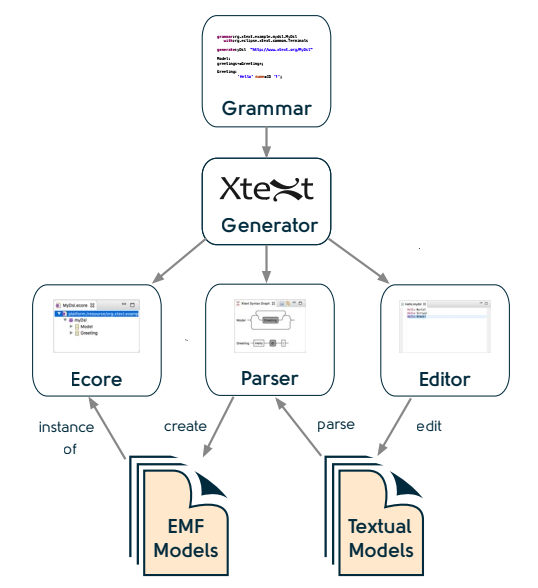
\includegraphics[width=0.6\textwidth]{img/ArquiteturaXtext.jpg}
    \label{fig:arqXtext}
    \fonte{\citeonline{XtextSirius:2017}.}
\end{figure}

Foram implementadas duas versões da gramática no protótipo da \ac{DSL}. 
A seguir as arquiteturas dessas implementações são descritas e pontua-se as diferenças entre elas. 
Essa abordagem foi definida tendo em vista que será realizada uma avaliação preliminar junto a um grupo focal. 
A partir dos resultados dessa avaliação, objetiva-se gerar uma versão final da gramática e, consequentemente, da arquitetura.

\begin{figure}[!htb]
    \centering
    \caption{Representação do modelo \textit{Ecore} da 1º versão da DSL.}
    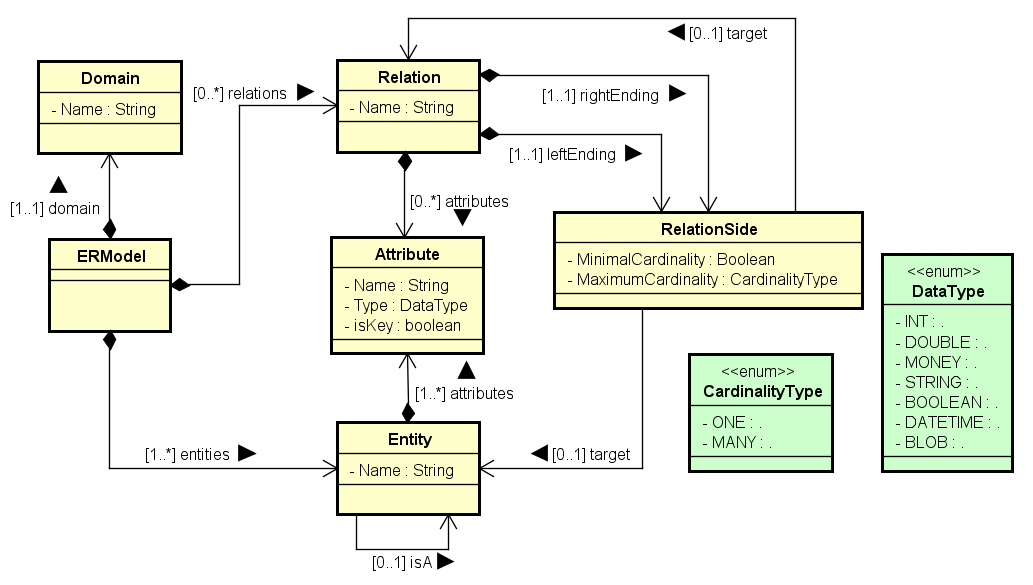
\includegraphics[width=1\textwidth]{img/erDslClassDiagram.png}
    \fonte{O autor.}
    \label{fig:ERDSL}
\end{figure}

A \autoref{fig:ERDSL} mostra um diagrama de classes para representar o modelo \textit{Ecore} da primeira versão criada para esta proposta. 
O elemento central do modelo é a classe \texttt{ERModel}, a qual corresponde por uma composição com outros elementos. 
O \texttt{ERModel} deve possuir um \texttt{Domain} associado, simbolizando o nome da base de dados modelada. 

Um \texttt{ERModel} também deve conter um ou mais elementos \texttt{Entity}. 
Um elemento \texttt{Entity} pode se relacionar com outro elemento \texttt{Entity}, cobrindo assim o conceito de generalização/especialização. 
Um \texttt{Entity} é também uma composição de uma ou mais classes \texttt{Attribute}. 
Definiu-se os tipos de dados em uma lista enumerada no elemento \texttt{DataType}.

Em seguida, um \texttt{ERModel} pode ser composto de uma ou mais relações, retratado como a classe \texttt{Relation}. 
Uma \texttt{Relation} por sua vez é formada por duas classes \texttt{RelationSide}, os quais são as cardinalidades da esquerda e da direita em uma relação. 
Estas duas relações possuem uma referência chamada \texttt{Target}, que pode ser uma \texttt{Entity} ou uma \texttt{Relation}. 
A inclusão da possibilidade de se referenciar uma \texttt{Relation} se faz necessário para cobrir a modelagem dos relacionamentos ternários.

Finalmente, tem-se o conceito das cardinalidades. 
Nele as cardinalidades possíveis, mantidas em atributos da \texttt{RelationSide}, são os tipos enumerados em \texttt{CardinalityType}, sendo \texttt{One} para um e \texttt{Many} para muitos. 
Por meio das regras da gramática garante-se que a cardinalidade mínima é implícita, tendo a palavra reservada \textit{zero} para simbolizar quando uma cardinalidade mínima pode ser nula. 
Isto significa que, em uma modelagem onde uma cardinalidade mínima \textit{zero} é omitida, assume-se que ela automaticamente é igual a um.

% \begin{figure} [!htb]
%     \centering
%     \caption{Representação do modelo ECORE da segunda versão da DSL.}
%     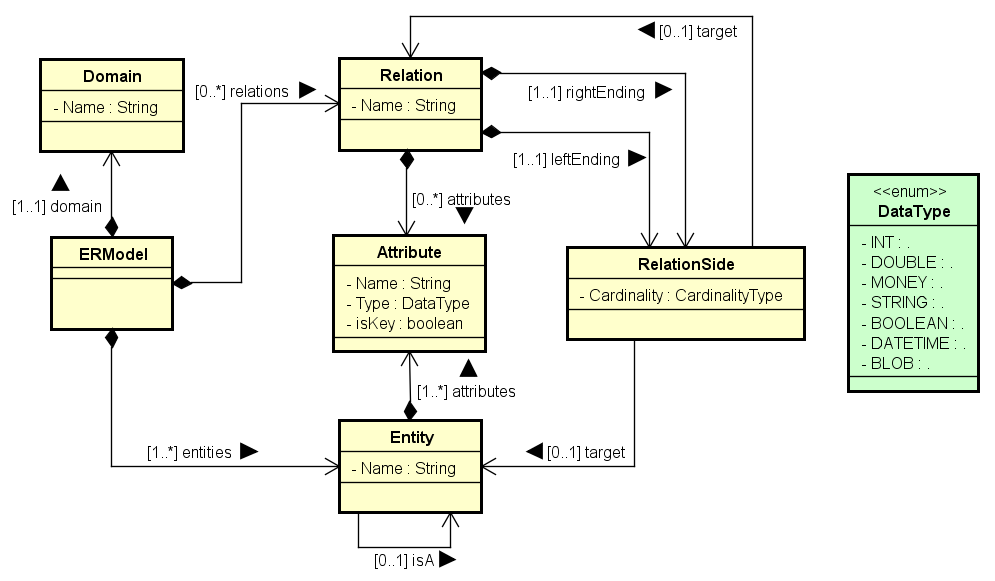
\includegraphics[width=0.8\textwidth]{img/erDsl2ClassDiagram.png}
%     \fonte{O autor.}
%     \label{fig:ERDSL2}
% \end{figure}

Estruturalmente o modelo \textit{Ecore} da segunda versão \ac{DSL} não muda significativamente.%, como pode-se observar na Figura \ref{fig:ERDSL2}. 
A única diferença com maior impacto é a opção pela definição da cardinalidade utilizando-se as quatro combinações possíveis como termos reservados, armazenados diretamente no atributo \texttt{Cardinality} de \texttt{RelationSide}.

%#################################################################
\section{Protótipo} \label{sec:protDSL}
%#################################################################
\definecolor{javared}{rgb}{0.6,0,0} % for strings
\definecolor{javagreen}{rgb}{0.25,0.5,0.35} % comments
\definecolor{javapurple}{rgb}{0.5,0,0.35} % keywords
\definecolor{javadocblue}{rgb}{0.25,0.35,0.75} % javadoc
\definecolor{verde}{rgb}{0.25,0.5,0.35}
\definecolor{jpurple}{rgb}{0.5,0,0.35}
\definecolor{darkgreen}{rgb}{0.0, 0.2, 0.13}


\lstdefinelanguage{Xtext}{
  sensitive = true,
  keywords={},
  keywords=[2]{ERModel, Domain, Attribute, Entity, Relation, RelationSide, DataType, CardinalityType},
  keywords=[3]{grammar, with, generate, Terminals, enum},
  otherkeywords={*, ?, +, *=, ?=, +=, |},
  keywordstyle=\color{black}\bfseries,
  keywordstyle=[2]\color{javadocblue}\bfseries,
  keywordstyle=[3]\color{javapurple}\bfseries,% for example
%   backgroundcolor=\color{cyan!10},
%   numbers=left,
%   stepnumber=1,
  numbersep=8pt,
  showstringspaces=false,
  breaklines=true,
  frame=top,
  comment=[l]{//},
  morecomment=[s]{/*}{*/},
  commentstyle=\color{black}\ttfamily,
  stringstyle=\color{javared}\ttfamily,
  morestring=[b]',
  morestring=[b]"
  }
  
  \lstdefinelanguage{ERDSL}{
  sensitive = true,
  keywords={},
  keywords=[2]{Domain, Entities, Relationships, isIdentifier, isRelatedWith, isA, zero, one, many},
  keywords=[3]{int, money, string, datetime, file},
  otherkeywords={*, ?, +, *=, ?=, +=, |},
  keywordstyle=\color{black}\bfseries,
  keywordstyle=[2]\color{javapurple}\bfseries,
  keywordstyle=[3]\color{javadocblue}\bfseries,% for example
%   backgroundcolor=\color{cyan!10},
%   numbers=left,
%   stepnumber=1,
  captionpos=t,
  numbersep=8pt,
  showstringspaces=false,
  breaklines=true,
  frame=top,
  comment=[l]{//},
  morecomment=[s]{/*}{*/},
  commentstyle=\color{black}\ttfamily,
  stringstyle=\color{javared}\ttfamily,
  morestring=[b]',
  morestring=[b]"
  }
  
  \lstdefinelanguage{BNF}{
  sensitive = true,
  keywords={},
  keywords=[2]{},
  otherkeywords={::= , |, <, >},
  keywordstyle=\color{javapurple}\bfseries,
  keywordstyle=[2]\color{javapurple}\bfseries,
  keywordstyle=[3]\color{javadocblue}\bfseries,% for example
%   backgroundcolor=\color{cyan!10},
%   numbers=left,
%   stepnumber=1,
  captionpos=t,
  numbersep=8pt,
  showstringspaces=false,
  breaklines=true,
  frame=top,
  comment=[l]{//},
  morecomment=[s]{/*}{*/},
  commentstyle=\color{darkgreen}\ttfamily,
  stringstyle=\color{javared}\ttfamily,
  morestring=[b]',
  morestring=[b]"
  }
  
  
  
  

Na fase atual do trabalho a linguagem a nível conceitual não se encontra totalmente finalizada. 
Existem tópicos relativos a validação de escopo, como no caso do tratamento de referências cruzadas indesejadas, e outras restrições inerentes ao modelo \ac{ER} que devem ser analisadas e então implementadas. 
A definição da \ac{DSL} criada é exibida na \autoref{fig:DSLvs1}.

\begin{figure}
    \centering
    \caption{Implementação da 1º versão da DSL.}
    \label{fig:DSLvs1}
    \begin{scriptsize}
    \begin{lstlisting}[language = Xtext , frame = trbl]
grammar org.xtext.unipampa.lesse.erdsl with org.eclipse.xtext.common.Terminals

generate erdsl "http://www.xtext.org/unipampa/lesse/erdsl/"

ERModel:
	domain=Domain ";"
	("Entities{") entities+=Entity+ ("};")
	("Relationships{") relations+=Relation* ("};");

Domain:
	"Domain" name=ID;

Entity:
	name=ID ("isA" isA+=[Entity])* 
	("{" attributes+=Attribute ("," attributes+=Attribute)* "}")?;

Attribute:
  name=ID ":" type=DataType (isKey?="isIdentifier")?;

Relation:
	(name=ID)? 
	("[" leftEnding=RelationSide 
	"isRelatedWith" 
	rightEnding=RelationSide "]")
	("{" attributes+=Attribute 
	("," attributes+=Attribute)* "}")*;
	
RelationSide:
	((minimalCardinality?="zero")?)	maximumCardinality=CardinalityType	
	target=[Entity] | target=[Relation];

enum DataType:
	INT="int" | DOUBLE="double" | MONEY="money" | STRING="string" | 
	BOOLEAN="boolean" | DATETIME="datetime" | BLOB="file";

enum CardinalityType:
	One="one" | Many="many";
    \end{lstlisting}
    \end{scriptsize}    
    \fonte{O autor.}
\end{figure}


O comando \texttt{grammar} especifica o nome da \ac{DSL}, enquanto que a instrução \texttt{with} declara uma herança de outra linguagem. 
No caso da gramática proposta, será utilizado uma gramática padrão do Xtext, chamada \texttt{Terminals}, a qual fornece algumas regras predefinidas como, por exemplo, a regra \texttt{ID} para identificadores ou \texttt{INT} para inteiros. 
O comando \texttt{generate} é a instrução que produz a \ac{AST} da linguagem.

A primeira regra, chamada de regra de entrada, define como é a estrutura geral da linguagem. 
Palavras e símbolos entre aspas duplas ou simples indicam as palavras reservadas. 
Por exemplo, o objeto \texttt{Entities} é obrigatoriamente precedido de "\texttt{Entities\{}". 
Este objeto representa uma espécie de \textit{container}, sendo isto indicado por meio do operador de atribuição \texttt{+=}. 
Ele é um objeto que pode conter outros objetos, no caso um ou mais \texttt{Entity} (entidades). 
É estabelecido que cada arquivo da \ac{DSL} deve também ser composto de um \texttt{Domain} (domínio) e zero ou mais \texttt{Relation} (relações). 

Para melhor entendimento, deve-se deixar claro que a multiplicidade é indicada por \texttt{*} (zero ou muitos), \texttt{+} (um ou muitos) ou \texttt{?} (zero ou um). 
Ao não se colocar nenhum desses operadores, implicitamente se espera então apenas uma ocorrência. 
Em relação às atribuições, quando apenas um \texttt{=} for especificado significa que o objeto da esquerda espera apenas um registro. 
Logo, para \texttt{+=} espera-se então zero, uma ou mais ocorrências. 

O objeto \texttt{Domain} é precedido de uma palavra reservada com o mesmo nome, seguido de um identificador. 
A entidade é definida pela palavra \texttt{Entity} e um nome identificador específico para este objeto. 
A definição de uma herança é opcional por meio da palavra reservada \texttt{isA}. 
Após a definição do nome, abre-se um corpo de chaves em que são especificados os atributos da entidade. 
Uma entidade deve conter ao menos um atributo, mas ele não precisa ser identificador por conta da possível existência de entidades fracas. 

As regras compostas só são realizadas devido à possibilidade de se agrupar expressões com o uso de parênteses, além da possibilidade de se utilizar outras regras por meio de referências cruzadas. 
Os colchetes entre a regra \texttt{Entity} servem para indicar que se almeja usar apenas o atributo \texttt{name} que identifica o objeto. 
% Se esse detalhe não for especificado então o compilador da linguagem interpretaria que é necessário aplicar toda a regra \texttt{Entity} novamente, ou seja, se iniciaria a definição de outra entidade entrando assim em um \textit{loop}. 
Os atributos das entidades são definidos por um nome, herdando a regra \texttt{ID} de \texttt{Terminals}, e atributos \texttt{isIdentifier} opcionais para simbolizar chaves primárias. 

A relação é definida, já dentro do corpo do bloco \texttt{Relationships}, com uma declaração opcional de sua identificação. 
Em seguida, são abertos colchetes e deve-se especificar dois elementos \texttt{RelationSide} como referência aos atributos \texttt{leftEnding} e \texttt{rightEnding}. 
Estes atributos representam os lados de uma relação. 
Estes objetos devem ser separados pela expressão \texttt{isRelatedWith}. 
Os lados da relação são definidos na regra \textit{RelationSide}, composta de dois atributos. 
O atributo \texttt{minimalCardinality} é opcional, indicado pelo operador \texttt{?}, e aceita apenas a palavra reservada \texttt{zero}. 
O atributo \texttt{maximumCardinality} aceita um objeto \texttt{CardinalityType}.

Os tipos de atributo estão contidos em uma lista enumerada chamada \texttt{DataType}, na esquerda fica a representação no modelo \textit{Ecore}. 
Na direita está a palavra reservada que é usada na linguagem. 
O símbolo condicional \texttt{|} significa o operador lógico \textit{OR} (ou) e serve para separar cada definição \texttt{<chave> = <valor>} como uma opção dentro da lista. 
Das três cardinalidades possíveis, duas estão definidas em outra lista enumerada chamada \texttt{CardinalityType}. 
Na \autoref{fig:DSLvs2} exibe a principal mudança entre as versões da \ac{DSL} proposta, a qual diz respeito a cardinalidade explícita. 
A \autoref{fig:ERDSLSyntax} e a \autoref{fig:ERDSL2Syntax} apresentam uma representação gráfica das sintaxes de ambas as gramáticas.

\begin{figure}[!htb]
    \centering
    \caption{Fragmento de implementação da 2º versão da DSL.}
    \label{fig:DSLvs2}
    \begin{footnotesize}
\begin{lstlisting}[language = Xtext , frame = trbl]
Relation:
	(name=ID)? ("[" leftEnding=RelationSide "relates" 
	rightEnding=RelationSide "]") ("{"attributes+=Attribute 
	("," attributes+=Attribute)* "}")*;

RelationSide:
	Cardinality=("(0,1)" | "(1,1)" | "(0,N)" | "(1,N)")
	target=[Entity] | target=[Relation];
    \end{lstlisting}
    \end{footnotesize} 
    \fonte{O autor}
\end{figure}

\begin{figure}[!htb]
    \centering
    \caption{Representação da sintaxe da 1º versão da DSL.}
    \label{fig:ERDSLSyntax}
    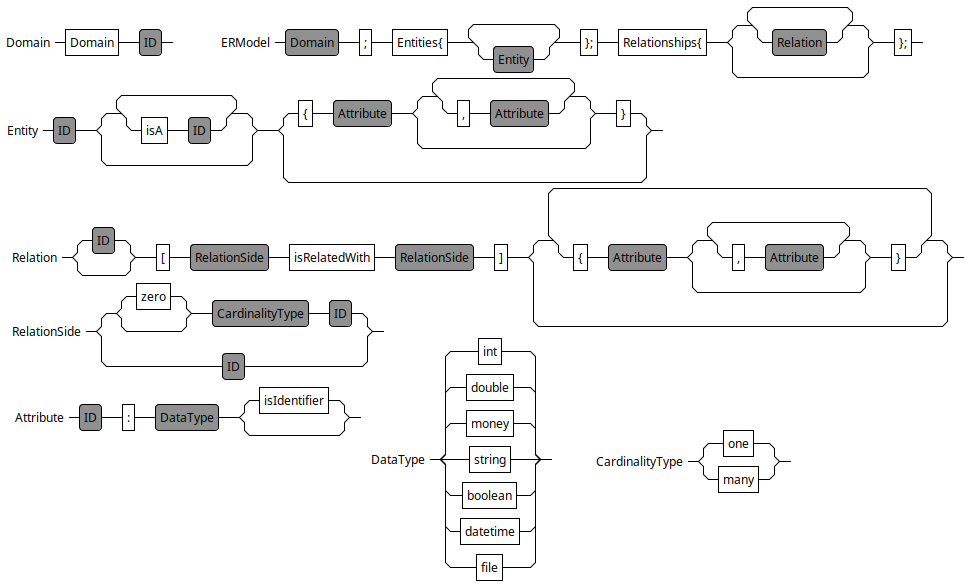
\includegraphics[width=\textwidth]{img/ERDSLSyntaxGraph.png}
    \fonte{O autor.}
\end{figure}

\begin{figure} [!htb]
    \centering
    \caption{Representação da sintaxe da 2º versão da DSL.}
    \label{fig:ERDSL2Syntax}
    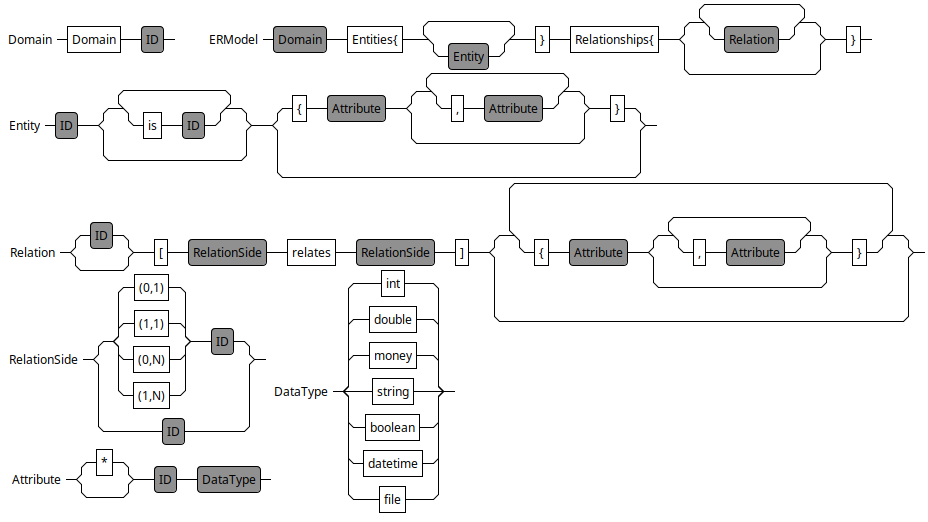
\includegraphics[width=\textwidth]{img/ERDSL2SyntaxGraph.png}
    \fonte{O autor.}
\end{figure}

Na \autoref{fig:DSLvs1Uso} mostra-se um exemplo de uso com um pequeno modelo que aborda uma universidade como domínio. 
Neste protótipo já se pode observar a modelagem de generalização/especialização, auto-relacionamento e relacionamento ternário.

% Para essa transformação existem regras que podem ser aplicadas, sendo que em alguns casos existem inclusive mais de uma opção. 
% Nestes casos estão sendo analisadas a melhores estratégias possíveis, uma vez que durante o processo de transformação será necessário se assumir algumas premissas.
Domain University;
\begin{figure}[!htb]
\centering
\caption{Exemplo de uso da 1º versão da DSL no RCP do Eclipse.}
\label{fig:DSLvs1Uso}
\begin{scriptsize}
\begin{lstlisting}[language = ERDSL, frame = trbl]
Entities{
	Person{ 
		PID: int isIdentifier, 
		Name: string
	}
	Teacher isA Person{ 
		Phone: int,
		Salary:money
	}
	Student isA Person{ 
		Course: string
	} 	
	OutsrcEmployee isA Person{
	    Company: string
	}
	Class{
		ClassID: int isIdentifier,
		Course: string,
		Semester: string
	}
	ClassRoom {
		ClassRoomID: int isIdentifier,
		Capacity: int
	}
};
\end{lstlisting}
\end{scriptsize}
    \fonte{O autor.}
\end{figure}

\begin{figure}[!htb]
\centering
\caption{Exemplo de uso da 1º versão da DSL no RCP do Eclipse.}
\label{fig:DSLvs1Uso}
\begin{scriptsize}
\begin{lstlisting}[language = ERDSL, frame = trbl]
Relationships{	 
	[many Student isRelatedWith many Class]
	TeacherClass [many Teacher isRelatedWith many Class]
	ClassSchedule [many TeacherClass isRelatedWith many ClassRoom]
	        {CSID: int isIdentifier, DayOfWeek: datetime, Discipline: string}
	Supervisor [one OutsrcEmployee isRelatedWith many OutsrcEmployee]
};
\end{lstlisting}
\end{scriptsize}
    \fonte{O autor.}
\end{figure}
É importante destacar que neste exemplo são modeladas seis entidades e quatro relacionamentos. 
Contudo, no processo de transformação para o modelo lógico espera-se que seja gerado um esquema textual com mais três entidades, inferindo-se isso através de, por exemplo, relacionamentos \textit{muitos para muitos}. 
Isso ocorreria, nesta amostra, no relacionamento sem identificação, atribuindo automaticamente a nova entidade o nome resultante da concatenação das duas entidades que se relacionam no conceitual. 
Também seriam criadas novas entidades a partir da derivação dos relacionamentos nomeados \texttt{TeacherClass} e \texttt{ClassShedule}, sendo que o último carateriza um relacionamento ternário.
Por fim, o auto-relacionamento \texttt{Supervisor} de \texttt{OutsrcEmployee} implicaria na adição de um novo atributo na entidade no novo modelo.

Com base nos modelos \textit{Ecore} gerados em tempo real, como o gerado a partir do modelo descrito anteriormente e exibido na \autoref{fig:EcoreRealTime}, já está sendo implementada a transformação do modelo conceitual para o lógico. 
A implementação desta transformação está sendo realizada utilizando-se a Xtend, uma \ac{GPL} baseada em Java.

\begin{figure} [!htb]
    \centering
    \caption{Fragmento do modelo \textit{Ecore} gerado em tempo de execução.}
    \label{fig:EcoreRealTime}
    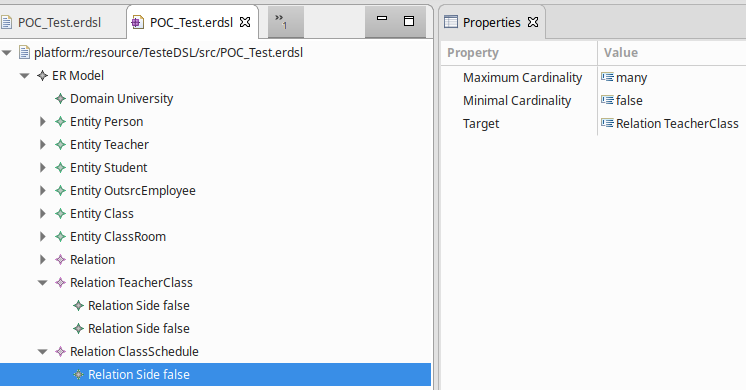
\includegraphics[width=\textwidth]{img/EcoreTempoReal.png}
    \fonte{O autor.}
\end{figure}


%#################################################################
\section{Avaliação Preliminar da Gramática} \label{sec:reqDSL}
%#################################################################
Esta seção descreve a avaliação preliminar conduzida para analisar as duas alternativas de gramática propostas, visando assim o seu aperfeiçoamento em uma versão final na solução. 
Para tanto, foi estabelecido a utilização de um grupo focal, um método de pesquisa qualitativa que objetiva gerar \textit{feedback} de um conjunto de pessoas em relação a um tema específico. 
O protocolo executado nesta etapa teve como base as diretrizes estabelecidas no trabalho de \citeonline{Kontio:2008}, que cobre a aplicação desse método no contexto da \ac{ES}. 

\subsection{Planejamento do Grupo Focal}

Durante o planejamento foi definido um protocolo que deveria ser seguido.
Neste protocolo, motivado pelo problema que era gerar uma versão definitiva da gramática da \ac{DSL} proposta, foram criados os documentos necessários para sua execução: \textbf{(I)} Termo de Consentimento Livre e Esclarecido; \textbf{(II)} Glossário de Termos; \textbf{(III)} Questionário de Perfil; \textbf{(IV)} Instrumentos da Discussão 1, 2 e 3; \textbf{(V)} Modelos das Gramáticas Avaliadas; \textbf{(VI)} Roteiro de Apresentação. 
Todos os modelos dos documentos produzidos estão incluídos no \autoref{ap:GRUPOFOCAL}.

\subsubsection{Definição do Participantes}

Tipicamente as avaliações que utilizam grupos focais devem ser constituídas de quatro (4) a seis (6) grupos focais individuais para que o rigor científico seja considerado verdadeiramente alto. 
O tamanho de cada grupo focal pode variar de três (3) a até doze (12) elementos, sendo mais comum esse número ficar entre quatro (4) e oito (8) participantes \cite{Kontio:2008}. 

Por questões de viabilidade de tempo e recursos humanos, para o presente estudo foi possível ser realizado apenas um grupo focal. 
Após a realização do convite houve a colaboração de treze (13) participantes, todos da área da \ac{ES}. 
Desse total, três (3) participantes eram alunos de graduação, nove (9) eram mestrandos e um (1) doutorando. 

Foi então aplicado o Questionário de Perfil, onde foi possível identificar que havia um nível equilibrado de conhecimento entre os participantes. 
Isso foi constatado pois todos já possuíam contato com \acp{DSL}, tendo utilizado esse tipo de linguagem, ao menos, durante a graduação.

\subsection{Execução do Grupo Focal}

O grupo focal foi realizado em 08/2019, nas dependências da UNIPAMPA, e teve duração de duas (2) horas. 
Iniciando com a exposição do roteiro que deveria ser seguido, onde houve a apresentação do objetivo do grupo focal e os conceitos básicos envolvidos, aconteceu o pedido para que os participantes realizassem a leitura e assinatura do Termo de Consentimento Livre e Esclarecido. 
Com o documento preenchido, foi dado continuidade ao roteiro previsto, 

A cada Instrumento de Discussão disponibilizado esperou-se até que os participantes respondessem de forma individual. 
Após, aconteceu uma discussão em grupo sobre o tema levantado. 
Todo o processo foi gravado em áudio e teve o suporte dos pesquisadores envolvidos neste estudo. 
Foi realizado também a transcrição das observações levantadas pelo debate que se seguiu, caracterizando assim as práticas de \textit{brainstorming}\footnote{Brainstorming é uma técnica utilizada para propor soluções a um problema específico. Consiste em uma reunião também chamada de tempestade de ideias, na qual os participantes devem ter liberdade de expor suas sugestões e debater sobre as contribuições dos colegas.} previstas em grupos focais. 

\subsection{Resultados do Grupo Focal}



\subsubsection{Discussão 1}

% \rowcolors{0}{}{}
% \begin{figure}[!htb]
% \centering
% \caption{Teste TiKZ.}
% % \pgfplotstableread{
% Instrumento           DT   DP    I   CP    CT
% Inst1           0       0       4       6       3     
% Inst2           0       0       4       6       3
% Inst3           0       0       4       6       3

% }\testdata

% \begin{tikzpicture}
% \begin{axis}[
%             legend cell align=left,
%             enlargelimits=0.15,
%             legend columns=1,
%             legend style={at={(0.5,-0.15)},anchor=north,draw=none},
%             xbar stacked,
%             xmin=0,
%             xmax=13,
%             xticklabel=\pgfmathprintnumber{\tick}\,$\%$,
%             ytick=data,
%             yticklabels from table={\testdata}{Instrumento}
%             ]
% \addlegendimage{empty legend}
% \addlegendentry{}
% \addplot [fill=red] table [x=DT, meta=Instrumento ,y expr=\coordindex] {\testdata};
% \addlegendentry{Discorda Totalmente}
% \addplot [fill=orange!90] table [x=DP, meta=Instrumento ,y expr=\coordindex] {\testdata};
% \addlegendentry{Discorda Parcialmente}
% \addplot [fill=yellow] table [x=I, meta=Instrumento ,y expr=\coordindex] {\testdata};
% \addlegendentry{Indiferente}
% \addplot [fill=black] table [x=CP, meta=Instrumento ,y expr=\coordindex] {\testdata};
% \addlegendentry{Concorda Parcialmente}
% \addplot [fill=green] table [x=CT, meta=Instrumento ,y expr=\coordindex] {\testdata};
% \addlegendentry{Concorda Totalmente}
% \end{axis}
% \end{tikzpicture}

\pgfplotstableread{ % Read the data into a table macro
Label                                Daily Weekly LessOften
Calendars\space And\space Reminders   0.51  0.24  0.25
Send/receive\space Texts              0.67  0.23  0.07
Make/receive\space Phone\space Calls  0.46  0.38  0.16
}\testdata

\begin{tikzpicture}
\begin{axis}[
            xbar stacked,   % Stacked horizontal bars
            xmin=0,         % Start x axis at 0
            ytick=data,     % Use as many tick labels as y coordinates
            yticklabels from table={\testdata}{Label}  % Get the labels from the Label column of the \datatable
]
\addplot [fill=cyan!20!green!40] table [x=Daily, meta=Label,y expr=\coordindex] {\testdata};   % "First" column against the data index
\addplot [fill=cyan!60!green!20] table [x=Weekly, meta=Label,y expr=\coordindex] {\testdata};
\addplot [fill=cyan!10] table [x=LessOften, meta=Label,y expr=\coordindex] {\testdata};
\end{axis}
\end{tikzpicture}
% \fonte{O autor.}
% \label{fig:Teste}
% \end{figure}

\subsubsection{Discussão 2}

\subsubsection{Discussão 3}





%#################################################################
\section{Lições do Capítulo} \label{sec:licDSL}
%#################################################################

Neste capítulo foram expostos os requisitos, as decisões de projeto e a arquitetura da \ac{DSL} proposta. 
Também foi demonstrado como o protótipo da versão preliminar da linguagem foi definido, bem como um exemplo de uso.

Até o momento o Xtext mostrou-se uma \ac{LW} capaz de suprir as necessidades iniciais do projeto, fornecendo suporte completo para a criação de gramáticas com notação \ac{BNF}, uma meta-sintaxe amplamente usada para expressar gramáticas livres de contexto como nas estruturas de linguagens de programação no geral. 
Além de prover a validação da gramática criada, foi gerado um \textit{plugin} tornando assim possível a realização do teste do protótipo em um \ac{RCP} Eclipse. 

%Assim, por meio disso o processo de modelagem com a nova linguagem criada ganhou recursos nativos como formatação, validação com base nas restrições descritas na gramática e \textit{syntax highlighting}. 
%É importante ressaltar que o \textit{plugin} somente pôde ser testado devido a integração nativa fornecida pelo Xtext com o \ac{EMF}, um conjunto de recursos do Eclipse para representar modelos e gerar código equivalente. 
%#################################################################
\chapter{Avaliação Experimental}\label{validacaoProposta}
%#################################################################
Este capítulo apresenta o experimento controlado que foi executado com a finalidade de verificar a viabilidade de uso da solução desenvolvida neste trabalho. 
Foram realizadas atividades que envolveram a execução de práticas de modelagem comparando os resultados da proposta deste estudo com a abordagem gráfica do BrModelo, uma ferramenta reconhecidamente utilizada no ensino de \acp{BD} nos cursos de graduação.

Sendo assim, foram realizadas análises quantitativas e qualitativas dos resultados coletados do experimento. 
Isso foi realizado a partir de métricas referentes ao esforço (tempo), precisão, revocação, Medida-F, bem como em questionários qualitativos para avaliação de itens referentes à utilidade percebida e facilidade de uso de ambas as abordagens.

A Seção \ref{sec:defExp} apresenta a definição da avaliação, seguida de seu escopo na Seção \ref{sec:escopoExp} e do planejamento na Seção \ref{ssec:planejExp}.
As atividades conduzidas na operação do experimento são relatadas na Seção \ref{ssec:operacaoExp}.
Finalmente, os resultados obtidos são apresentados na Seção \ref{sec:resultExp} e os lições do capítulo pontudas na Seção \ref{sec:licoesExp}.

%#################################################################
\section{Definição da Avaliação} \label{sec:defExp}
%#################################################################
Segundo \citeonline{Wohlin:2012}, a \ac{ESE} trata da utilização de abordagens científicas para o desenvolvimento, evolução, manutenção e validação de software. 
A \ac{ESE} usa métodos científicos para fazer pesquisa e para também tomar decisões sobre mudanças na forma de desenvolver software.

Na \ac{ESE} é possível realizar medições controladas, objetivas e orientadas a verificação, caracterizando assim a análise quantitativa. 
Da mesma forma, também é possível fazer observações naturalísticas, entrevistas e questionários, sendo essa uma abordagem orientada a descoberta e caracterizada como análise qualitativa.

As diferentes técnicas que a \ac{ESE} engloba podem ser classificadas em dois grandes grupos: estudos experimentais e observacionais. 
Enquanto nas técnicas observacionais o pesquisador conduz a investigação sobre um objeto de estudo sem qualquer ação sobre ele, nas técnicas experimentais existe essa intervenção pela inclusão, exclusão ou modificação de algum fator estudado, procurando comparar o comportamento dos conjuntos de amostras perante algum cenário predefinido.

%#################################################################
\section{Escopo} \label{sec:escopoExp}
%#################################################################

Houve a escolha por uma abordagem experimental para avaliação da proposta, a qual foi executada com base na definição de um planejamento prévio. 
Tendo como base o modelo proposto por \citeonline{Wohlin:2012}, esta etapa do estudo contemplou as seguintes atividades: \textbf{(i)} Planejamento (Objetivo, questões de pesquisa, etc); \textbf{(ii)} Operação (Preparação, Execução); \textbf{(iii)} Coleta dos Dados; \textbf{(iv)} Análise dos Dados e \textbf{(v)} Relatório e discussão dos resultados.

%#################################################################
\section{Planejamento} \label{ssec:planejExp}
%#################################################################
Nesta seção será apresentado o objetivo, as questões de pesquisa, o contexto, a hipótese,  a seleção dos participantes, os instrumentos utilizados, o \textit{design} experimental executado e as ameaças à validade. 

\subsection{Definição do Objetivo} \label{ssec:defObj}

O experimento tem por objetivo obter evidências a partir da comparação de duas abordagens para a modelagem de \acp{BD} relacionais, uma de forma gráfica e outra textual. 
Os intitulados tratamentos, foram: 
\textbf{(i)} Tratamento controle: a ferramentas BrModelo, de abordagem gráfica, e \textbf{(ii)} Tratamento experimental: ferramenta ERText, de abordagem textual e resultado da proposta deste trabalho.

O propósito do experimento é avaliar a viabilidade do uso de uma abordagem textual para apoio no processo de ensino-aprendizagem de modelagem conceitual de \ac{BD} relacionais.

\subsection{Questões de Pesquisa} \label{ssec:questPesq}
Para a discussão dos resultados obtidos neste experimento optou-se pela formulação de quatro (4) \acp{QP} que tivessem relação com as atividades executadas no experimento, bem como na percepção de uso dos participantes. 
\begin{itemize}
    \small
    \item \textbf{QP1.} Qual abordagem demanda mais esforço médio durante a atividade de modelagem conceitual?
    \item \textbf{QP2.} Qual o nível da qualidade dos modelos produzidos utilizando a abordagem gráfica e a textual?
    \item \textbf{QP3.} Qual é a percepção dos sujeitos quanto a utilidade e facilidade de uso da \ac{DSL} proposta?
    \item \textbf{QP4.} Qual a avaliação dos sujeitos em relação à representação dos construtores \ac{ER} suportados na \ac{DSL} proposta?
\end{itemize}

\subsection{Contexto} \label{ssec:contxExp}

O contexto do experimento é caracterizado conforme quatro (4) dimensões:

\begin{itemize}
    \item \textbf{Processo:} Foi utilizada uma abordagem \textit{in-vitro}, uma vez que as tarefas foram realizadas em laboratório sob condições controladas e sem atividades \textit{online}.
    \item \textbf{Participantes:} Os participantes foram estudantes de graduação e pós-graduação em cursos de computação.
    \item \textbf{Realidade:} O experimento abordou um problema real, ou seja, a diferença no esforço dos indivíduos na modelagem conceitual de \acp{BD} relacionais, a qualidade dos artefatos produzidos e a percepção dos sujeitos usando duas abordagens distintas.
    \item \textbf{Generalidade:} Esta avaliação está inserida em um contexto específico, envolvendo alunos de computação e modelagem de \ac{BD}. Contudo, as ideias gerais deste experimento podem ser replicadas em outro conjunto de participantes, abordagens ou \acp{DSL} que suportem modelagem de \acp{BD}.
\end{itemize}

\subsection{Formulação de Hipótese} \label{ssec:hipExp}

Geralmente a análise das hipóteses de um experimento controlado tem como base métricas e teste estatísticos.
Com base nos dados coletados durante a execução de um experimento as hipóteses são testadas para verificar se é possível aceitar uma alternativa à hipótese nula \cite{Wohlin:2012}.

Para a formulação das hipóteses foram levadas em consideração as duas primeiras \acp{QP}. 
Em relação a \ac{QP}1, sobre o esforço médio necessário utilizando cada abordagem, as hipóteses são as seguintes:

\textbf{Hipótese Nula:} $H_0 : \mu Tempo_G = \mu Tempo_T :$ Não há diferença de esforço médio entre as abordagens textual e gráfica durante a modelagem conceitual de \acp{BD} relacionais. 

\textbf{Hipótese Alternativa:} $H_{1} : \mu Tempo_T \neq Tempo_G :$  Existe diferença de esforço médio entre as abordagens textual e gráfica durante a modelagem conceitual de \acp{BD} relacionais. 

Em relação a \ac{QP}2, sobre a efetividade de modelagem utilizando cada abordagem, as hipóteses são as seguintes:

\textbf{Hipótese Nula:} $H_0 : \mu Efetividade_G = \mu Efetividade_T :$ Não há diferença de efetividade entre as abordagens textual e gráfica durante a modelagem conceitual de \acp{BD} relacionais. 

\textbf{Hipótese Alternativa:} $H_{1} : \mu Efetividade_T \neq \mu Efetividade_G :$ Há diferença de efetividade entre as abordagens textual e gráfica durante a modelagem conceitual de \acp{BD} relacionais. 

Para a avaliação referente ao esforço foram utilizados o teste de normalidade Shapiro-Wilk e o Teste T pareado para amostras dependentes, em que foi levado em consideração os tempos coletados durante a execução das atividades de modelagem do experimento. 
O método Shapiro-Wilk testa a hipótese nula de que uma distribuição é normal, mediante o cálculo do valor $W$, onde após é então verificado na tabela do teste\footnote{\url{http://www.uel.br/projetos/experimental/pages/arquivos/Probabilidades\_Shapiro.pdf}} se ocorre a rejeição ou aceitação da hipótese. 
O cálculo do método Shapiro-Wilk é dado conforme a fórmula da Equação \ref{eq:Shapiro}: 

\begin{equation}
\label{eq:Shapiro}
%\[ 
W = \frac{\left(\sum_{i=1}^{n} a_ix_{(i)}\right)^2}{\sum_{i=1}^{n}\left(x_i -\overline{x}\right)} 
%\]
\end{equation}

Uma forma simplificada do Teste T pareado para amostras dependentes
se dá conforme a fórmula da Equação \ref{eq:TestT}:

\begin{equation}
\label{eq:TestT}
%\[ 
t = \frac{m}{s/\sqrt{n}} 
%\]
\end{equation}

Nesta fórmula o \textit{\textbf{m}} e o \textit{\textbf{s}} são a média e o desvio padrão da diferença (\textbf{\textit{d}}), respectivamente. 
O \textit{\textbf{n}} corresponde ao tamanho de \textbf{\textbf{d}}, ou seja, o tamanho da amostra.
Este teste de hipótese é usado para comparar as médias de duas amostras relacionadas, ou seja, quando se possui dois valores (par de valores) para uma mesma amostra. 
Contudo, para comparar as médias dos dois conjuntos de dados emparelhados, as diferenças entre todos os pares devem ser calculadas primeiro.
O nível de significância alfa ($\alpha$) utilizado foi de cinco por cento (5\%).
Os cálculos Shapiro-Wilk e Teste T pareado foram realizados com o suporte da linguagem R\footnote{https://www.rdocumentation.org/packages/stats/versions/3.6.1/topics/shapiro.test}\footnote{https://www.rdocumentation.org/packages/stats/versions/3.6.1/topics/t.test}.

Para os testes da efetividade foram adotados os mesmos métodos estatísticos, porém ao invés do uso da métrica de tempo foi necessário outra grandeza.
Sendo assim, foram realizados os cálculos da Medida-F, a qual é derivada a partir dos valores de \textit{Precisão} e \textit{Revocação}, para cada um dos modelos produzidos nas abordagens.
O cálculo da Medida-F leva em consideração variáveis conhecidas como \textit{Verdadeiros Positivos}, \textit{Falsos Positivos} e \textit{Falsos Negativos}.
\begin{itemize}
    \item \textbf{Verdadeiros Positivos} (VP): Quantidade de elementos corretamente modelados com a utilização da abordagem.
    \item \textbf{Falsos Positivos} (FP): Quantidade de de elementos incorretamente modelados
    com a abordagem.
    \item \textbf{Falsos Negativos} (FN): Quantidade de elementos não modelados com a abordagem.
\end{itemize}
A partir da identificação das variáveis é possível então calcular a \textit{Precisão}, \textit{Revocação} e \textit{Medida-F} de cada modelo conforme as fórmulas:
\begin{itemize}
    \item \textbf{Precisão} (P): $\frac{VP}{VP~+~FP}$ 
    \item \textbf{Revocação} (R):$\frac{VP}{VP~+~FN}$ 
    \item \textbf{Medida-F} (F): $\frac{2~*~(P~*~ R)}{P~+~R}$ 
\end{itemize}


\subsection{Seleção dos Participantes} \label{ssec:participExp}

Os sujeitos do experimento foram selecionados por amostragem não probabilística, indicada para estudos exploratórios.
Esse tipo de amostragem se caracteriza a partir da escolha proposital de indivíduos com uma ou mais características que interessam ao objeto de estudo. 

Neste experimento houve a participação de vinte e sete (27) alunos de graduação (Ciência da Computação e Engenharia de Software) e pós-graduação (Engenharia de Software) da Universidade Federal do Pampa - Campus Alegrete. 
Entre os participantes haviam catorze (14) alunos matriculados em disciplinas de \ac{BD}. 

Depois de identificar os potenciais participantes, aconteceu a definição da data para a execução do experimento, o que incluía o treinamento nas duas abordagens.
Além disso, antes do treinamento seria solicitado aos participantes que respondessem a um questionário de perfil para nivelamento. 

A partir dos dados extraídos dos questionários houve a distribuição aleatória dos sujeitos em dois grupos. 
Os grupos foram compostos por treze (13) e catorze (14) sujeitos em razão do número total de participantes ser ímpar,  e também procurou-se manter um nível equilibrado de habilidades entre os conjuntos dos sujeitos.

\subsection{\textit{Design} da Avaliação} \label{ssec:designExp}

Segundo \citeonline{Wohlin:2012}, um experimento deve atender alguns conceitos fundamentais: tipo de projeto padrão, bloqueio, balanceamento e randomização. 

\textbf{Tipo de Projeto Padrão}: Existem alguns tipos possíveis para o projeto padrão em um experimento, e este estudo adotou o de um (1) \textit{Fator} com dois (2) \textit{Tratamentos}. O \textit{Fator} foi a modelagem de \acp{BD} relacionais, e os \textit{Tratamentos} foram as duas (2) abordagens utilizadas (gráfica e textual).

\textbf{Bloqueio}: Este item se refere ao fato dos participantes do experimento poderem possuir diferentes níveis de experiência na área de modelagem e projeto de \acp{BD}. 
Em razão disso foi aplicado um questionário de perfil para o nivelamento dos sujeitos.

\textbf{Balanceamento}: Os participantes foram separados em dois grupos com níveis semelhantes de conhecimento. 
Desta forma, ambas as abordagens foram executadas por grupos homogêneos.

\textbf{Randomização}: Os sujeitos foram alocados aleatoriamente para cada grupo e abordagem. 
Os sujeitos executaram os dois tratamentos, caracterizando um \textit{design} pareado. 
A ordem de execução das abordagens para cada grupo também foi definida aleatoriamente.

A \autoref{fig:designExp} exibe o desenho experimental da avaliação. 
Após todas as atividades realizadas pelo sujeitos utilizando os tratamentos, ocorre a coleta dos resultados.
Esta etapa consiste na avaliação qualitativa feita pelos sujeitos e no salvamento dos modelos produzidos pela aplicação dos tratamentos. 
Estes modelos servem posteriormente para uma avaliação qualitativa.
Por fim, é realizada a etapa de análise, onde os dados são compilados e examinados com o objetivo de se extrair conclusões.

\begin{figure}[!htb]
    \centering
    \caption{\textit{Design} do experimento.}
    \label{fig:designExp}
    

\tikzset{every picture/.style={line width=0.75pt}} %set default line width to 0.75pt        

\begin{tikzpicture}[x=0.75pt,y=0.75pt,yscale=-1,xscale=1]
%uncomment if require: \path (0,327.1999969482422); %set diagram left start at 0, and has height of 327.1999969482422




%Shape: Ellipse [id:dp6331487904311781] 
\draw  [line width=1.5]  (448.63,88.9) .. controls (448.63,72.61) and (468.97,59.4) .. (494.05,59.4) .. controls (519.13,59.4) and (539.46,72.61) .. (539.46,88.9) .. controls (539.46,105.19) and (519.13,118.4) .. (494.05,118.4) .. controls (468.97,118.4) and (448.63,105.19) .. (448.63,88.9) -- cycle ;


%Shape: Rectangle [id:dp03801896284105699] 
\draw  [line width=1.5]  (249.43,28) -- (319.43,28) -- (319.43,68) -- (249.43,68) -- cycle ;

%Shape: Ellipse [id:dp583213096835353] 
\draw  [line width=1.5]  (99.3,85.85) .. controls (99.3,65.22) and (125.04,48.5) .. (156.8,48.5) .. controls (188.56,48.5) and (214.3,65.22) .. (214.3,85.85) .. controls (214.3,106.48) and (188.56,123.2) .. (156.8,123.2) .. controls (125.04,123.2) and (99.3,106.48) .. (99.3,85.85) -- cycle ;

%Straight Lines [id:da1799424135415575] 
\draw    (214.3,85.85) -- (246.81,50.98) ;
\draw [shift={(248.17,49.52)}, rotate = 493] [fill={rgb, 255:red, 0; green, 0; blue, 0 }  ][line width=0.75]  [draw opacity=0] (8.93,-4.29) -- (0,0) -- (8.93,4.29) -- cycle    ;

%Straight Lines [id:da17029537209985257] 
\draw    (214.3,85.85) -- (246.9,125.23) ;
\draw [shift={(248.17,126.77)}, rotate = 230.38] [fill={rgb, 255:red, 0; green, 0; blue, 0 }  ][line width=0.75]  [draw opacity=0] (8.93,-4.29) -- (0,0) -- (8.93,4.29) -- cycle    ;

%Straight Lines [id:da39402523544663426] 
\draw  [dash pattern={on 4.5pt off 4.5pt}]  (319.71,108.71) -- (358.51,70.41) ;
\draw [shift={(359.93,69)}, rotate = 495.36] [fill={rgb, 255:red, 0; green, 0; blue, 0 }  ][line width=0.75]  [draw opacity=0] (8.93,-4.29) -- (0,0) -- (8.93,4.29) -- cycle    ;

%Straight Lines [id:da7992081880522388] 
\draw  [dash pattern={on 4.5pt off 4.5pt}]  (319.43,68) -- (358.78,106.32) ;
\draw [shift={(360.21,107.71)}, rotate = 224.24] [fill={rgb, 255:red, 0; green, 0; blue, 0 }  ][line width=0.75]  [draw opacity=0] (8.93,-4.29) -- (0,0) -- (8.93,4.29) -- cycle    ;

%Right Arrow [id:dp4964522106990972] 
\draw  [line width=1.5]  (4.3,23.74) -- (60.47,23.74) -- (60.47,1.77) -- (96.12,85.85) -- (60.47,169.92) -- (60.47,147.96) -- (4.3,147.96) -- cycle ;

%Shape: Rectangle [id:dp003852149638719382] 
\draw  [line width=1.5]  (361.43,28) -- (431.43,28) -- (431.43,68) -- (361.43,68) -- cycle ;

%Shape: Rectangle [id:dp0126542660109914] 
\draw  [line width=1.5]  (361.43,108.75) -- (431.43,108.75) -- (431.43,148.75) -- (361.43,148.75) -- cycle ;

%Shape: Rectangle [id:dp4954877903085966] 
\draw  [line width=1.5]  (249.43,108.75) -- (319.43,108.75) -- (319.43,148.75) -- (249.43,148.75) -- cycle ;
%Straight Lines [id:da3442884963113835] 
\draw    (431.43,68) -- (448.31,76.5) ;
\draw [shift={(450.1,77.4)}, rotate = 206.72] [fill={rgb, 255:red, 0; green, 0; blue, 0 }  ][line width=0.75]  [draw opacity=0] (8.93,-4.29) -- (0,0) -- (8.93,4.29) -- cycle    ;

%Straight Lines [id:da6883068419855551] 
\draw    (431.43,108.75) -- (448.93,101.19) ;
\draw [shift={(450.77,100.4)}, rotate = 516.65] [fill={rgb, 255:red, 0; green, 0; blue, 0 }  ][line width=0.75]  [draw opacity=0] (8.93,-4.29) -- (0,0) -- (8.93,4.29) -- cycle    ;

%Rounded Rect [id:dp5928061300931144] 
\draw  [line width=1.5]  (575,20.46) .. controls (575,17.11) and (577.71,14.4) .. (581.06,14.4) -- (599.24,14.4) .. controls (602.59,14.4) and (605.3,17.11) .. (605.3,20.46) -- (605.3,157.34) .. controls (605.3,160.69) and (602.59,163.4) .. (599.24,163.4) -- (581.06,163.4) .. controls (577.71,163.4) and (575,160.69) .. (575,157.34) -- cycle ;

%Straight Lines [id:da6932528701926595] 
\draw    (539.46,88.7) -- (569.92,88.68) ;
\draw [shift={(571.92,88.68)}, rotate = 539.96] [fill={rgb, 255:red, 0; green, 0; blue, 0 }  ][line width=0.75]  [draw opacity=0] (8.93,-4.29) -- (0,0) -- (8.93,4.29) -- cycle    ;

%Straight Lines [id:da7950818392289087] 
\draw    (43.3,181.2) -- (43.3,154.2) ;
\draw [shift={(43.3,152.2)}, rotate = 450] [color={rgb, 255:red, 0; green, 0; blue, 0 }  ][line width=0.75]    (10.93,-4.9) .. controls (6.95,-2.3) and (3.31,-0.67) .. (0,0) .. controls (3.31,0.67) and (6.95,2.3) .. (10.93,4.9)   ;

%Straight Lines [id:da5784112946450906] 
\draw    (493.97,181.53) -- (493.97,126.53) ;
\draw [shift={(493.97,124.53)}, rotate = 450] [color={rgb, 255:red, 0; green, 0; blue, 0 }  ][line width=0.75]    (10.93,-4.9) .. controls (6.95,-2.3) and (3.31,-0.67) .. (0,0) .. controls (3.31,0.67) and (6.95,2.3) .. (10.93,4.9)   ;


% Text Node
\draw (47.67,85) node  [align=left] {27 Sujeitos};
% Text Node
\draw (156.8,70) node [scale=0.8] [align=left] {Randomização };
% Text Node
\draw (156.8,86.5) node [scale=0.8] [align=left] {de };
% Text Node
\draw (156.8,103) node [scale=0.8] [align=left] {Balanceamento};
% Text Node
\draw (284.43,56.5) node [scale=0.8] [align=left] {\textbf{Gráfica}};
% Text Node
\draw (284.43,39.5) node [scale=0.8] [align=left] {Abordagem};
% Text Node
\draw (396.43,39.5) node [scale=0.8] [align=left] {Abordagem};
% Text Node
\draw (396.43,56.5) node [scale=0.8] [align=left] {\textbf{Gráfica}};
% Text Node
\draw (396.43,120.25) node [scale=0.8] [align=left] {Abordagem};
% Text Node
\draw (396.43,137.25) node [scale=0.8] [align=left] {\textbf{Textual}};
% Text Node
\draw (284.43,120.25) node [scale=0.8] [align=left] {Abordagem};
% Text Node
\draw (284.43,137.25) node [scale=0.8] [align=left] {\textbf{Textual}};
% Text Node
\draw (494.05,75.15) node [scale=0.8] [align=left] {Coleta};
% Text Node
\draw (494.05,88.9) node [scale=0.8] [align=left] {de};
% Text Node
\draw (494.05,102.65) node [scale=0.8] [align=left] {Resultados};
% Text Node
\draw (590.15,88.9) node [scale=0.8,rotate=-270] [align=left] {Análise dos Resultados};
% Text Node
\draw (43,190) node [scale=0.8] [align=left] {Questionário};
% Text Node
\draw (43,206) node [scale=0.8] [align=left] {de};
% Text Node
\draw (43,221) node [scale=0.8] [align=left] {Perfil};
% Text Node
\draw (493.67,221) node [scale=0.8] [align=left] {Avaliação Qualitativa};
% Text Node
\draw (493.67,206) node [scale=0.8] [align=left] {e};
% Text Node
\draw (493.67,192) node [scale=0.8] [align=left] {Modelos Produzidos};


\end{tikzpicture}

    \fonte{Adaptado de \citeonline{Bernardino:2016}.}
\end{figure}



\subsection{Instrumentação} \label{ssec:instExp}

Como a participação no experimento foi voluntária, preparou-se um \ac{TCLE} aos participantes para o registro da concordância de todos os sujeitos na execução das atividades, apresentado no Apêndice \ref{ap:TermoExp}.
O questionário de perfil criado e aplicado para o balanceamento dos grupos e está presente no Apêndice \ref{ap:QuestPerfilExp}.
Também foi elaborado um glossário para conceitos que foram utilizados na apresentação de abertura do experimento e durante os treinamentos, exposto no Apêndice \ref{ap:GlossarioExp}.

Com a finalidade de fornecer o suporte aos participantes da avaliação, foram providenciados instrumentos descrevendo o passo a passo com exemplos, exibidos nos Apêndices \ref{ap:StepBrModeloExp} e \ref{ap:StepERDSLExp}, para o uso das ferramentas utilizadas no experimento (BrModelo e ERText). 
Além disso, foi realizado um treinamento que incluía vídeos com tutoriais de uso das abordagens em cada ferramenta. 
Os vídeos demostravam como se deveria iniciar a modelagem, exemplos dos construtores previstos nos problemas que eles teriam que resolver e as recomendações para o salvamento dos artefatos produzidos. 

Foram elaborados dois (2) instrumentos que continham um problema cada, com níveis similares de complexidade, os quais deveriam ser modelados e também anotados os horários de começo e término da atividade. 
Estes instrumentos estão nos Apêndices \ref{ap:Inst1Exp} e \ref{ap:Inst2Exp}. 
Para a posterior avaliação por parte dos sujeitos foram criados outros dois (2) instrumentos. 
O primeiro apresentava sete (7) atributos de qualidade com base na ISO/IEC 25010\footnote{https://www.iso.org/standard/35733.html}, uma norma para qualidade de produtos de software, e serviu para avaliar as abordagens das duas ferramentas do ponto de vista dos sujeitos que executaram as atividades de modelagem \ac{ER}.
Este instrumento é apresentado no Apêndice \ref{ap:Inst3Exp}.
O segundo instrumento serviu para a avaliação da representação dos construtores da solução proposta neste estudo, e está disposto no Apêndice \ref{ap:Inst4Exp}. 
Os dados gerados por estes instrumentos serviram para responder as \acp{QP} qualitativas definidas para este experimento.

Ademais, foi também gerado um ambiente de trabalho igual para todos os sujeitos do experimento. 
Para tanto, criou-se uma máquina virtual que utilizava o sistema operacional Xubuntu\footnote{https://xubuntu.org/}, uma distribuição Linux derivada do Ubuntu que utiliza o ambiente gráfico XFCE. 
Neste ambiente foram disponibilizados os materiais de apoio citados anteriormente, bem como as ferramentas de modelagem \ac{ER}. 
Para evitar possíveis influências externas as máquinas virtuais não tinham acesso com a Internet, garantindo assim que os sujeitos não poderiam realizar consultas à conteúdos externos. 
Dessa forma, foi possível assegurar que todos os sujeitos realizaram as mesmas tarefas, e nas mesmas condições.

\subsection{Ameaças à Validade} \label{ssec:validadeExp}

Objetivando que a avaliação tenha um resultado válido para o experimento proposto, foi necessário analisar e discutir as ameaças à validade, bem como as estratégias utilizadas para mitigá-las.
Para a listagem das possíveis ameaças foram utilizadas os tópicos e recomendações levantadas no trabalho de \citeonline{Wohlin:2012}. 
Essas ameaças seguiram o padrão proposto e foram divididas em quatro (4) categorias, sendo: validade do construto, validade interna, validade externa e validade de conclusão.

\subsubsection{Validade do Construto}

A validade do construto diz respeito ao \textit{design} do experimento e a fatores sociais.

\textit{\textbf{Explicação pré-operacional inadequada}}: Esta ameaça está relacionada com o fato do experimento não ter o objetivo dos artefatos suficientemente definidos antes de serem traduzidos em medidas ou tratamentos. 
Para mitigar essa ameaça foi comparado o esforço em tempo de cada abordagem, bem como foi realizada a verificação da efetividade de acordo com os conceitos de \textit{Precisão} e \textit{Revocação} da \textit{Medida-F}.

\textit{\textbf{Interação de diferentes tratamentos}}. Se os sujeitos estiverem envolvidos em mais de um estudo, os tratamentos dos diferentes estudos poderão interagir e reverberar nos resultados finais. 
Como este experimento seguiu um \textit{design} pareado, todos os sujeitos realizaram os dois tratamentos. 
Contudo, não foi identificado aprendizado entre a execução das atividades.
Isto pode ser verificado por meio da normalidade das distribuições analisadas das amostras de esforço e efetividade, as quais demonstram que os resultados mantiveram-se semelhantes como um todo.

\textit{\textbf{Predição das hipóteses}}: 
Quando os sujeitos participam de um experimento é possível que tentem descobrir qual é o objetivo ou o resultado pretendido do experimento. 
Este fato pode trazer viés ao comportamento, positivamente ou negativamente, dependendo da hipótese antecipada.
Para mitigar essa ameaça os sujeitos não foram informados sobre maiores detalhes do experimento \textit{e.g.} perguntas de pesquisa, hipóteses, objetivos e propósito.


\subsubsection{Validade Interna}

Ameaças à validade interna são influências que podem afetar as variáveis independentes em relação à causalidade, sem o conhecimento do pesquisador. 

\textit{\textbf{História}}: Há o risco de algum período temporal específico ter influência na realização do experimento. 
Para mitigar esta ameaça, e em razão do experimento ser realizado em ambiente acadêmico, todo o processo foi executado no mês de agosto, em que no geral os alunos não estão necessariamente sobrecarregados com atividades acadêmicas \textit{e.g.} provas e trabalhos.

\textit{\textbf{Maturação}}: Essa é a ameaça que ocorre em relação aos sujeitos reagirem de maneiras diferentes com o passar do tempo. 
Exemplos são quando os sujeitos são afetados negativamente (cansaço ou tédio) ou positivamente (aprendizado) durante o curso do experimento.
Para mitigar essa ameaça foi comunicado desde o início aos sujeitos que poderiam encerrar a sua participação no momento que quisessem, sem qualquer tipo de penalização.

\textit{\textbf{Testes}}: Se os testes forem repetidos, os sujeitos podem responder de maneira diferente em momentos diferentes, pois sabem como o teste é realizado. 
Se houver necessidade de familiarização com os testes, é importante que os resultados do teste não sejam devolvidos ao sujeito, para assim não apoiar o aprendizado não intencional. 
Não houve necessidade de repetição das atividades, uma vez que as mesmas foram executadas uma vez por participante em cada tratamento.

\textit{\textbf{Instrumentação}}: Essa ameaça está relacionada aos artefatos usados para a execução da experiência, como formulários de coleta de dados, etc.
Se estes foram mal projetados, a experiência é afetada negativamente.
Para combater essa ameaça, todos os artefatos foram verificados e validados previamente em reuniões entre os pesquisadores envolvidos neste trabalho.
Além disso, foi realizado um estudo piloto para validar o protocolo planejado para o experimento.

\subsubsection{Validade Externa}

As ameaças à validade externa são as condições relacionadas a replicação do experimento.

\textit{\textbf{Sujeitos do experimento}}: Os sujeitos selecionados para o experimento podem não representar um grupo significativo para a área de estudo. 
Buscando tentar mitigar essa ameaça o experimento foi realizado com estudantes de Engenharia de Software e Ciência da Computação, e logo, inseridos no contexto de uso da modelagem conceitual de \acp{BD} relacionais.
Porém, o fato da amostra ter menos de trita (30) elementos é uma ameaça estatística na área analisada, e não foi possível mitigar este fato.

\textit{\textbf{Interação dos sujeitos com os artefatos de avaliação}}: Essa é a ameaça relacionada a aplicação dos artefatos de avaliação do experimento com os sujeitos.
Dependendo do momento isto pode afetar os resultados.
Se, por exemplo, um questionário for realizado alguns dias após a execução do experimento, as pessoas tendem a responder de maneira diferente do que fariam momentos após as atividades.

\textit{\textbf{Interação de configuração e tratamento}}: São ameaças relacionadas ao fato de se usar uma configuração ou material não representativo. 
Para mitigar essa ameaça, foi utilizada uma documentação com base em \textit{templates} e modelos tradicionais encontrados em material de ensino de \acp{BD}. 
Além disso, os artefatos foram validados com dois especialistas da área de Engenharia de Software.

Um ponto importante quanto a validade externa é que as ameaças podem ser reduzidas tornando o ambiente experimental o mais realista possível. 
Por outro lado, a realidade nem sempre é homogênea. 
Porém,  mais importante é definir e relatar as características do ambiente, como experiência da equipe, ferramentas, métodos de avaliação e a aplicabilidade em um contexto específico \cite{Wohlin:2012}.

\subsubsection{Validade da Conclusão}

As ameaças à validade da conclusão estão relacionadas com questões que afetam a capacidade de se inferir uma conclusão correta sobre as relações entre os tratamentos e o resultado de um experimento.

\textit{\textbf{Baixo poder estatístico}}: Uma possível ameaça nesta categoria é o baixo poder estatístico.
Para tentar mitigar esta ameaça foi adotado alguns métodos estatísticos como o teste de normalidade Shapiro-Wilk, o Teste T pareado como teste de hipótese para amostras dependentes, e a Medida-F para análise qualitativa dos modelos produzidos.

\textit{\textbf{Confiabilidade das medições}}: A confiabilidade das medições utilizadas tem impacto direto na validade do experimento como um todo. Para mitigar essa ameaça foram realizadas medições objetivas que não dependiam de julgamento subjetivo (esforço, medido em tempo, e Medida-F). 
Por outro lado, as métricas utilizadas para a avaliação qualitativa ainda serviram como insumo complementar na discussão dos resultados obtidos.

\textit{\textbf{Ambiente experimental}}: O experimento deve ser realizado em um ambiente controlado, procurando evitar influẽncias externas. Para mitigar esta possível ameaça os
participantes foram orientados que não poderia ocorrer conversas durante todo o tempo das atividades, nem saídas do ambiente ou acesso a dispositivos eletrônicos.


%#################################################################
\section{Operação do Experimento} \label{ssec:operacaoExp}
%#################################################################

A operação do experimento pode ser dividida em duas (2) etapas: preparação e execução.
Esta seção descreve de forma geral as ações realizadas em ambas as etapas.

%#################################################################
\subsection{Preparação}
%#################################################################

Inicialmente ocorreram reuniões entre os pesquisadores envolvidos para definição geral do planejamento e do modo de operação que deveria ser adotado.
Buscando captar uma amostra significativa para o objeto do estudo, optou-se pelo contato com a docente responsável por ministrar as disciplinas de Banco de Dados (Engenharia de Software) e Banco de Dados I (Ciência da Computação) em 2019/2.
Após reuniões para explicar os objetivos do trabalho, houve a concordância quanto a viabilidade do experimento.
Com os objetivos iniciais alinhavados, a docente que colaborou realizou a divulgação dos questionários de perfil via plataforma Moodle para os alunos matriculados.
Com os alunos do mestrado não foi possível o envio antecipado dos questionários, e por conta disso o mesmo foi aplicado no dia do experimento.

Com as respostas daqueles que retornaram o formulário de nivelamento, tantos os alunos de Engenharia de Software quanto de Ciência da Computação, começou-se a realizar com antecedência o nivelamento dos possíveis candidatos a participar do experimento.
Após a elaboração de todos os artefatos que seriam utilizados no experimento, os mesmos foram analisados e validados em conjunto pelos pesquisadores envolvidos neste estudo, havendo ainda nesse percurso a necessidade de adequação de alguns instrumentos quanto as sugestões e eventuais correções necessárias.

%#################################################################
\subsection{Execução}
%#################################################################

No dia do experimento a primeira atividade realizada foi uma breve apresentação inicial onde era informado que o experimento era de caráter não avaliativo.
Com isto esclarecido, era então disponibilizado o \ac{TCLE} (\ref{ap:TermoExp}) para todos os participantes.
Após a assinatura do \ac{TCLE}, foram distribuídos os questionários de perfil para aqueles participantes que ainda não haviam o preenchido anteriormente.
Foi constatado que não havia fortes discrepâncias entre os níveis de conhecimento dos sujeitos, demonstrando assim que no geral era uma amostra homogênea.

Antes da divisão randômica dos grupos foi realizada então a fase de treinamento. 
Durante essa etapa foram apresentadas ambas as ferramentas que seriam utilizadas, passando uma visão geral de operação e respondendo a possíveis dúvidas que pudessem surgir.
O treinamento incluía a exibição de vídeos demonstrando as ferramentas, primeiramente do BrModelo e após do editor Eclipse com o \textit{plugin} da \ac{DSL} proposta, respectivamente, com cerca de nove (9) e onze (11) minutos. 

Então, deu-se início a fase de modelagem dos problemas propostos.
Todos os participantes receberam o Instrumento 1 (\ref{ap:Inst1Exp}) e foram informados com qual ferramenta deveriam desenvolver a solução.
Foi solicitado que cada sujeito anotasse no instrumento sua identificação e o horário de início da tarefa.
Não foi estipulado nenhum tempo limite para o término e, conforme os sujeitos finalizavam a modelagem, era pedido que cumprissem as orientações inclusas no material de apoio para o salvamento dos artefatos gerados.
Com os modelos salvos, os instrumentos eram recolhidos e passava-se para a próxima tarefa descrita no Instrumento 2 (\ref{ap:Inst2Exp}), porém sendo necessário o uso da abordagem inversa a que haviam utilizado inicialmente.

Ao término dos instrumentos que continham os problemas de modelagem, foi entregue os instrumentos de avaliação qualitativa (\ref{ap:Inst3Exp} e \ref{ap:Inst4Exp}). 
Conforme os participantes finalizavam o preenchimento da avaliação, eram então liberados.
Com a conclusão do experimento por parte dos vinte e sete (27) sujeitos, encerrou-se o experimento e partiu-se para a etapa de tabulação e análise dos resultados.

%#################################################################
\section{Resultados} \label{sec:resultExp}
%#################################################################

Esta seção relata a análise dos resultados obtidos a partir dos material coletado no experimento. 
%Com base nos dados foi possível responder as questões de pesquisa e, quando fosse o caso, as hipóteses relacionadas.
É importante salientar que toda a análise estatística foi realizada com apoio da Linguagem R\footnote{RStudio: \url{https://rstudio.com}}, bem como nas recomendações do livro referência de \citeonline{Triola:2017}.

\subsection{Esforço}

Para responder a \ac{QP}1 referente ao esforço de uso das abordagens, os tempos foram extraídos dos instrumentos. 
A \autoref{tab:TemposGeral} exibe os valores associados aos sujeitos, bem como a ordem de execução das abordagens.

\begin{table}[!htb]
    \caption{Tempos de execução de cada abordagens.}
    \label{tab:TemposGeral}
    \centering
    \tiny
    \begin{tabular}{c|cc|cc}
    \bottomrule
    \rowcolor[HTML]{C0C0C0}
    \multicolumn{1}{r}{Sujeito} &
    \multicolumn{2}{c}{\textbf{Abordagem (minutos)}} &
    \multicolumn{2}{c}{\textbf{Abordagem (minutos)}}
    \\ 
    \hline
    01	&	Gráfica	&	25	&	Textual	&	48	\\
    02	&	Gráfica	&	26	&	Textual	&	45	\\
    03	&	Gráfica	&	28	&	Textual	&	38	\\
    04	&	Gráfica	&	21	&	Textual	&	28	\\
    05	&	Gráfica	&	31	&	Textual	&	20	\\
    06	&	Gráfica	&	42	&	Textual	&	26	\\
    07	&	Gráfica	&	60	&	Textual	&	58	\\
    08	&	Gráfica	&	22	&	Textual	&	36	\\
    09	&	Gráfica	&	22	&	Textual	&	28	\\
    10	&	Gráfica	&	22	&	Textual	&	30	\\
    11	&	Gráfica	&	20	&	Textual	&	28	\\
    12	&	Gráfica	&	18	&	Textual	&	30	\\
    13	&	Gráfica	&	21	&	Textual	&	15	\\
    14	&	Gráfica	&	12	&	Textual	&	16	\\
    15	&	Textual	&	60	&	Gráfica	&	28	\\
    16	&	Textual	&	18	&	Gráfica	&	22	\\
    17	&	Textual	&	56	&	Gráfica	&	27	\\
    18	&	Textual	&	38	&	Gráfica	&	28	\\
    19	&	Textual	&	60	&	Gráfica	&	28	\\
    20	&	Textual	&	41	&	Gráfica	&	46	\\
    21	&	Textual	&	33	&	Gráfica	&	20	\\
    22	&	Textual	&	57	&	Gráfica	&	35	\\
    23	&	Textual	&	32	&	Gráfica	&	17	\\
    24	&	Textual	&	35	&	Gráfica	&	28	\\
    25	&	Textual	&	38	&	Gráfica	&	26	\\
    26	&	Textual	&	20	&	Gráfica	&	25	\\
    27	&	Textual	&	18	&	Gráfica	&	12	\\
    \toprule
    \end{tabular}
    \fonte{O autor.}
\end{table}

A partir dos valores brutos dos tempos foi calculada a diferença para ser possível realizar o teste de normalidade Shapiro-Wilk.
Por ser um teste estatístico, esta técnica tem como produto a medida do valor-$p$.
Para este teste foi adotado um nível de significância $\alpha$~=~5\%. 
Isso significa que se o valor-$p$ for menor que 5\% ($p$ < 0.05), a hipótese nula de que a distribuição é normal deve ser rejeitada.

Após os cálculos com o conjunto das diferenças dos tempos chegou-se a um valor-$p$ de 0.606530.
Como valor-$p$ > $\alpha$, a hipótese nula foi aceita, concluindo assim que os dados são normalmente distribuídos.
Em outras palavras, a diferença entre a amostra de dados e a distribuição normal não é grande o suficiente para ser estatisticamente significativa.

É importante ressaltar que quanto maior o valor-$p$, mais ele suporta uma hipótese nula. 
No caso do resultado obtido a chance de erro do tipo 1 (rejeitar uma hipótese nula que é correta) é muito alta, podendo ser traduzida em 60,65\% (0.606530).

Ainda em relação ao teste de normalidade, o valor de \textit{W} calculado foi de 0.970178, estando dentro do intervalo aceito do valor crítico de 95\% (0.9242 : 1.0000). 
Isto significa que existe 95\% de chances da amostra ter origem em uma população normal.
A \autoref{fig:DistTempo} apresenta uma representação visual da distribuição analisada.

\begin{figure}[!htb]
    \centering
    \caption{Distribuição amostral referente ao esforço.}
    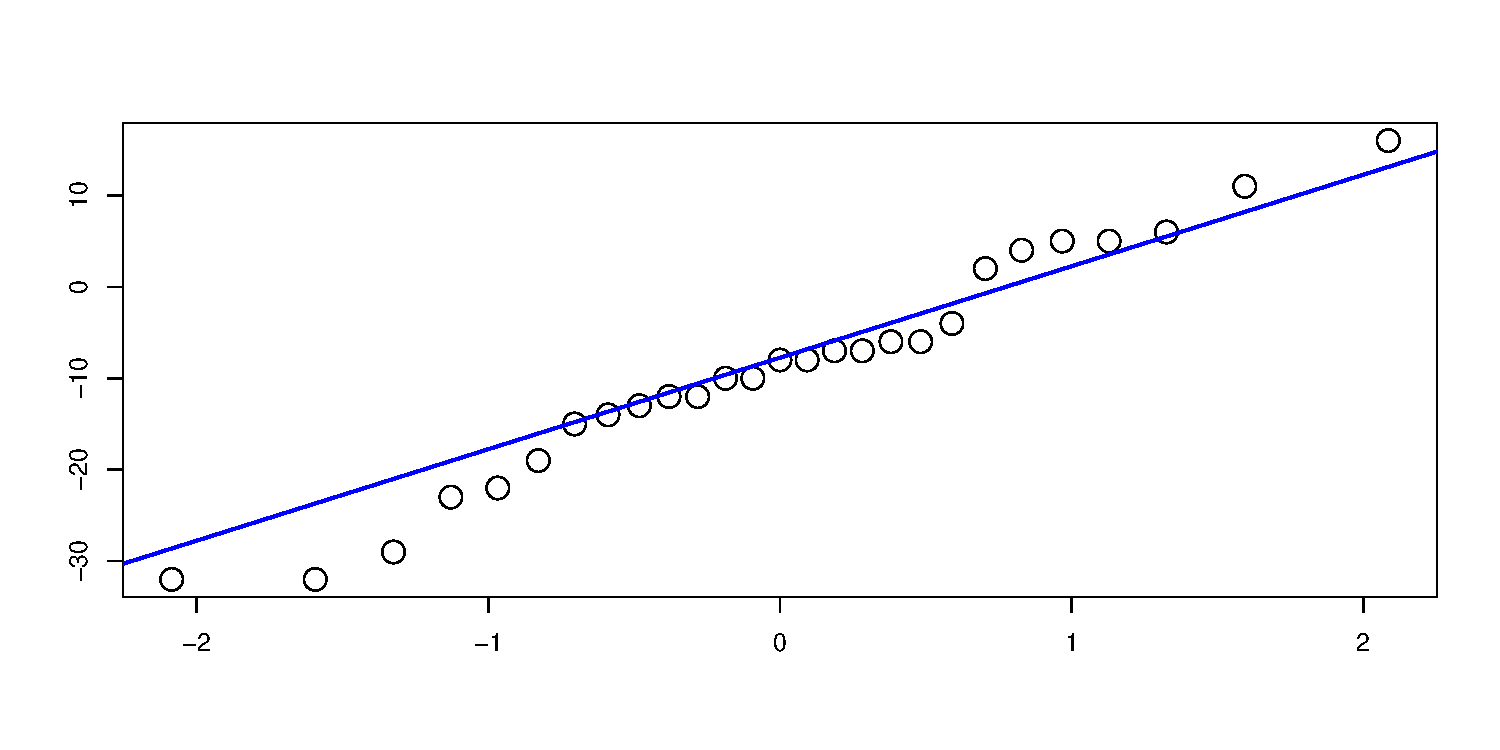
\includegraphics[width=0.7\textwidth]{ResultsExp/DistribuicaoAmostraTempo}
    \label{fig:DistTempo}
    \fonte{O autor.}
\end{figure}

Tendo sido a amostra testada quanto à sua normalidade, foi possível realizar o teste da primeira hipótese estabelecida neste experimento. 
No teste T pareado para amostras dependentes foi utilizado um nível de significância $\alpha$~=~5\%, com o qual se chegou a uma medida de 0.000962084 para o valor-$p$. 
Por ser um teste bicaudal, ou seja, que inclui uma igualdade na sua hipótese nula, esse valor-$p$ mostra evidências suficientes para garantir a rejeição da afirmativa de $H_0 : \mu Tempo_G = \mu Tempo_T$.
Logo, a hipótese alternativa de que as abordagens possuem esforços diferentes é aceita, pois segundo o teste essa diferença é estatisticamente significativa.

A \autoref{tab:TemposGeralMedidas} mostra os valores que possibilitam uma análise de dispersão. A \autoref{fig:boxplotTempo} exibe um \textit{boxplot} com a variação de dados observados por meio destes dados. 
Com base nestes dados e na sua representação visual, é possível verificar que, em média, a abordagem gráfica leva vantagem sobre a abordagem textual. 

\begin{table}[!htb]
    \caption{Medidas relacionadas ao esforço médio.}
    \label{tab:TemposGeralMedidas}
    \centering
    \footnotesize
    \begin{tabular}{l|lc|lc}
    \bottomrule
    \rowcolor[HTML]{C0C0C0}
    \multicolumn{1}{c}{\textbf{}} &
    \multicolumn{2}{c}{\textbf{Abordagem}}
    \\
    \rowcolor[HTML]{C0C0C0}
    \multicolumn{1}{c}{\textbf{Medida}} &
    \multicolumn{1}{c}{\textbf{Gráfica}} &
    \multicolumn{1}{c}{\textbf{Textual}}
    \\
    \hline
        Limite Inferior 	&	12.00   &   15.00   \\
        1\degree Quartil	&	21.00	&   27.00   \\
        Média	            &	26.37	&   35.26   \\
        Mediana	            &	25.00   &   33.00   \\
        3\degree Quartil	&	28.00   &   43.00   \\
        Limite superior	    &	60.00   &   60.00   \\
        Desvio Padrão	    &  	10.12	&	14.03	\\
    \toprule
    \end{tabular}
    \fonte{O autor.}
\end{table}


\begin{figure}[!htb]
    \centering
    \caption{Tempos medidos nos tratamentos.}
    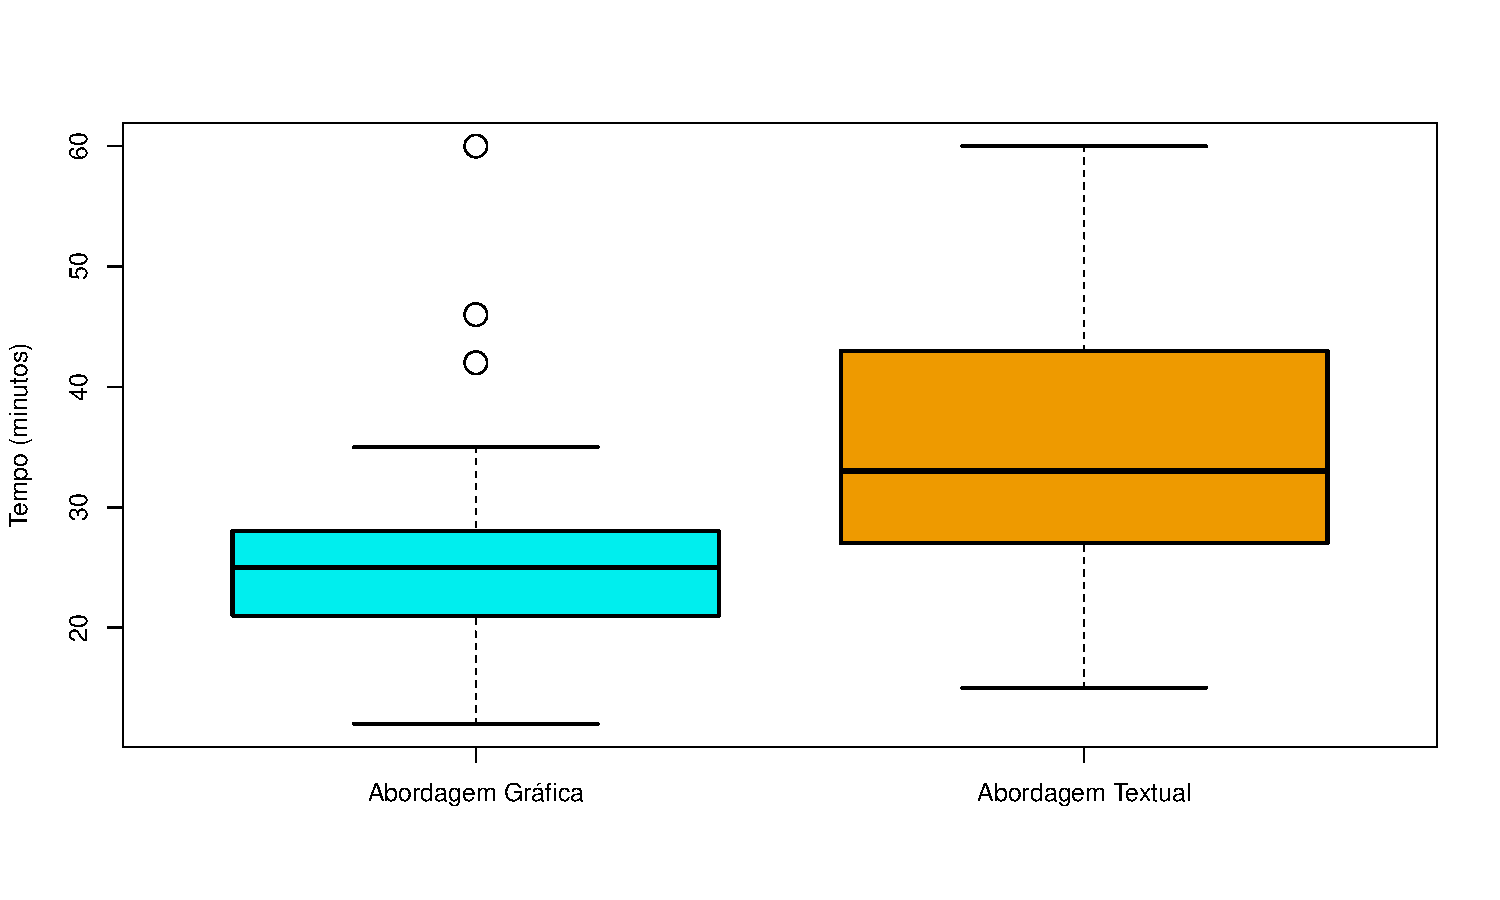
\includegraphics[width=0.8\textwidth]{ResultsExp/BoxPlotTempo}
    \label{fig:boxplotTempo}
    \fonte{O autor.}
\end{figure}



\subsection{Efetividade}
Para responder a \ac{QP}2 referente a efetividade do uso das abordagens, os artefatos produzidos pelos sujeitos foram avaliados conforme os modelos de referência estabelecidos.

\rowcolors{1}{gray!15}{white}
\begin{landscape}
\begin{table}[!htb]
    \caption{Avaliação dos modelos produzidos no experimento.}
    \label{tab:ResultsModelosIndividual}
    \centering
    \footnotesize
    
    \begin{tabular}{l|cc|ccc|cc|ccc}
    \bottomrule
    \rowcolor[HTML]{C0C0C0}
    \multicolumn{1}{l}{} &
    \multicolumn{5}{c}{\textbf{Abordagem Gráfica}} &
    \multicolumn{5}{c}{\textbf{Abordagem Textual}}
    \\ 
    \hline
    \rowcolor[HTML]{C0C0C0}
    \textbf{P} & \textbf{IM} & \textbf{IR} & \textbf{Precisão (\%)} & \textbf{Revocação (\%)} & \textbf{Medida-F (\%)} &
    \textbf{IM} & \textbf{IR} & \textbf{Precisão (\%)} & \textbf{Revocação (\%)} & \textbf{Medida-F (\%)}
    \\
    01	&	23	&	17	&	73.91	&	36.96	&	49.28	&	29	&	24	&	82.76	&	60.00	&	69.57	\\
    02	&	41	&	33	&	80.49	&	84.62	&	82.50	&	67	&	41	&	61.19	&	87.23	&	71.93	\\
    03	&	38	&	28	&	73.68	&	71.79	&	72.73	&	50	&	42	&	84.00	&	89.36	&	86.60	\\
    04	&	36	&	25	&	69.44	&	64.10	&	66.67	&	44	&	32	&	72.73	&	68.09	&	70.33	\\
    05	&	32	&	26	&	81.25	&	66.67	&	73.24	&	31	&	28	&	90.32	&	59.57	&	71.79	\\
    06	&	32	&	24	&	75.00	&	61.54	&	67.61	&	38	&	36	&	94.74	&	76.60	&	84.71	\\
    07	&	37	&	32	&	86.49	&	69.57	&	77.11	&	23	&	21	&	91.30	&	52.50	&	66.67	\\
    08	&	41	&	34	&	82.93	&	87.18	&	85.00	&	44	&	39	&	88.64	&	97.50	&	92.86	\\
    09	&	36	&	31	&	86.11	&	79.49	&	82.67	&	36	&	30	&	83.33	&	63.83	&	72.29	\\
    10	&	38	&	33	&	86.84	&	84.62	&	85.71	&	20	&	19	&	95.00	&	40.43	&	56.72	\\
    11	&	40	&	35	&	87.50	&	76.09	&	81.40	&	29	&	25	&	86.21	&	62.50	&	72.46	\\
    12	&	53	&	33	&	62.26	&	84.62	&	71.74	&	53	&	42	&	79.25	&	89.36	&	84.00	\\
    13	&	37	&	34	&	91.89	&	73.91	&	81.93	&	48	&	35	&	72.92	&	87.50	&	79.55	\\
    14	&	46	&	33	&	71.74	&	84.62	&	77.65	&	36	&	29	&	80.56	&	61.70	&	69.88	\\
    15	&	29	&	27	&	93.10	&	69.23	&	79.41	&	41	&	37	&	90.24	&	78.72	&	84.09	\\
    16	&	33	&	25	&	75.76	&	54.35	&	63.29	&	34	&	30	&	88.24	&	75.00	&	81.08	\\
    17	&	39	&	26	&	66.67	&	66.67	&	66.67	&	45	&	37	&	82.22	&	78.72	&	80.43	\\
    18	&	40	&	35	&	87.50	&	89.74	&	88.61	&	45	&	43	&	95.56	&	91.49	&	93.48	\\
    19	&	27	&	24	&	88.89	&	52.17	&	65.75	&	51	&	32	&	62.75	&	80.00	&	70.33	\\
    20	&	25	&	24	&	96.00	&	52.17	&	67.61	&	34	&	25	&	73.53	&	62.50	&	67.57	\\
    21	&	36	&	33	&	91.67	&	71.74	&	80.49	&	35	&	30	&	85.71	&	75.00	&	80.00	\\
    22	&	34	&	29	&	85.29	&	74.36	&	79.45	&	44	&	38	&	86.36	&	80.85	&	83.52	\\
    23	&	42	&	32	&	76.19	&	82.05	&	79.01	&	41	&	27	&	65.85	&	57.45	&	61.36	\\
    24	&	28	&	19	&	67.86	&	41.30	&	51.35	&	26	&	19	&	73.08	&	47.50	&	57.58	\\
    25	&	36	&	32	&	88.89	&	82.05	&	85.33	&	38	&	35	&	92.11	&	74.47	&	82.35	\\
    26	&	34	&	13	&	38.24	&	33.33	&	35.62	&	31	&	18	&	58.06	&	38.30	&	46.15	\\
    27	&	31	&	26	&	83.87	&	56.52	&	67.53	&	37	&	31	&	83.78	&	77.50	&	80.52	\\
    \toprule
    \end{tabular}
    \begin{tablenotes}
    \tiny
    \item Legenda: IM (\textit{Itens Modelados}) IR (\textit{Itens Relevantes})
    \end{tablenotes}
    \fonte{O autor.}
\end{table}
\end{landscape}

Nesta avaliação foi utilizada a Medida-F, uma medida proveniente da área de reconhecimento de padrões e recuperação de informação. 
A Medida-F representa a combinação da precisão e revocabilidade observada de um resultado em relação à uma referência.

Por definição, essa combinação se refere à fração de instâncias recuperadas que são relevantes (precisão) e a fração de instâncias relevantes que são recuperadas  (revocabilidade).
A \autoref{tab:ResultsModelosIndividual} exibe estes valores associados obtidos pelos sujeitos, separados pelos tratamentos realizados.

Após a obtenção dos valores da Medida-F de cada modelo, foi realizado o teste de normalidade Shapiro-Wilk.
Após os cálculos com o conjunto das diferenças da Medida-F de cada modelo, chegou-se a um valor-$p$ de 0.404455.
Com este resultado obtido a chance de erro do tipo 1 (rejeitar uma hipótese nula que é correta) pode ser muito alta, podendo ser traduzida em 40,45\% (0.404455).

Como o valor-$p$ > $\alpha$, a hipótese nula foi aceita, constatando assim que os dados são normalmente distribuídos, isto é, a diferença entre a amostra de dados e a distribuição normal não é grande o suficiente para ser estatisticamente significativa.
A \autoref{fig:distMedidaF} apresenta a representação visual da distribuição do conjunto de diferenças da Medida-F dos modelos.

\begin{figure}[!htb]
    \centering
    \caption{Distribuição amostral referente a efetividade.}
    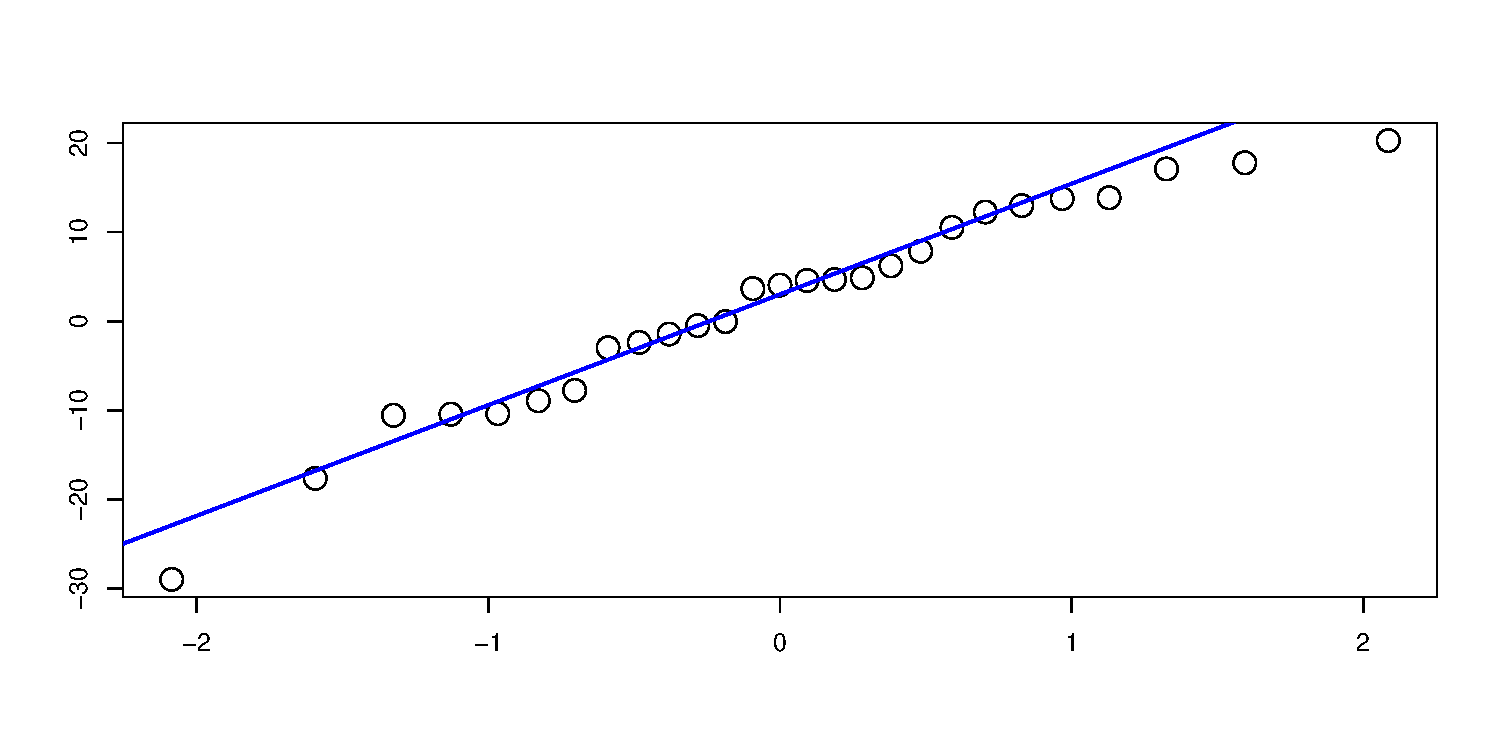
\includegraphics[width=0.7\textwidth]{ResultsExp/DistribuicaoAmostraFScore}
    \label{fig:distMedidaF}
    \fonte{O autor.}
\end{figure}

Após a amostra ser testada quanto à sua normalidade, foi realizado o teste da segunda hipótese definida neste experimento. 
Desta vez, no teste T pareado para amostra dependentes, novamente foi utilizado um nível de significância $\alpha$~=~5\%, com o qual se chegou a uma medida de 0.396468 para o valor-$p$. 

Pela afirmativa original incluir uma igualdade, caracterizando também este teste como bicaudal, chegou-se a conclusão que o valor-$p$ calculado demonstra que não há evidências suficientes para garantir a rejeição da afirmativa da hipótese nula original, denotada como $H_0 : \mu Efetividade_G = \mu Efetividade_T$.
Logo, a hipótese nula de que as abordagens possuem efetividades iguais é aceita, pois segundo o teste a diferença média da Medida-F entre os tratamentos não é estatisticamente significativa.

A \autoref{tab:ResultsModelosGeral} mostra medidas médias dos valores avaliados, e também fornecem a possibilidade para a realização de uma análise de dispersão. 


\begin{table}[!htb]
    \caption{Médias gerais da avaliação dos modelos produzidos no experimento.}
    \label{tab:ResultsModelosGeral}
    \centering
    \tiny
    
    \begin{tabular}{l|cc|ccc|cc|ccc}
    \bottomrule
    \rowcolor[HTML]{C0C0C0}
    \multicolumn{1}{l}{} &
    \multicolumn{5}{c}{\textbf{Abordagem Gráfica}} &
    \multicolumn{5}{c}{\textbf{Abordagem Textual}}
    \\ 
    \hline
    \rowcolor[HTML]{C0C0C0}
    Medida & \textbf{IM} & \textbf{IR} & \textbf{P (\%)} & \textbf{R (\%)} & \textbf{MF (\%)} &
    \textbf{IM} & \textbf{IR} & \textbf{P (\%)} & \textbf{R (\%)} & \textbf{MF (\%)}
    \\
Limite Inferior	&	23.00	&	13.00	&	38.24	&	33.33	&	35.62	&	20.00	&	18.00	&	58.06	&	38.30	&	46.15	\\
1\degree Quartil	&	32.00	&	25.00	&	73.80	&	59.03	&	67.10	&	32.50	&	26.00	&	73.30	&	60.85	&	69.72	\\
Média	&	35.70	&	28.26	&	79.61	&	68.57	&	72.79	&	38.89	&	31.30	&	81.50	&	70.88	&	74.73	\\
Mediana	&	36.00	&	29.00	&	82.93	&	71.74	&	77.11	&	38.00	&	31.00	&	83.78	&	75.00	&	72.46	\\
3\degree Quartil	&	39.50	&	33.00	&	87.50	&	82.05	&	81.66	&	44.50	&	37.00	&	89.44	&	80.43	&	82.93	\\
Limite Superior	&	53.00	&	35.00	&	96.00	&	89.74	&	88.61	&	67.00	&	43.00	&	95.56	&	97.50	&	93.48	\\
Desvio Padrão	&	6.33	&	5.63	&	11.94	&	15.39	&	12.16	&	9.97	&	7.30	&	10.44	&	15.36	&	10.94	\\
 \toprule
    \end{tabular}
    \begin{tablenotes}
    \tiny
    \item Legenda: IM (\textit{Itens Modelados}) IR (\textit{Itens Relevantes})
    P (\textit{Precisão}) R (\textit{Revocação})
    MF (\textit{Medida-F})
    \end{tablenotes}
    \fonte{O autor.}
\end{table}

O \textit{boxplot} da \autoref{fig:BoxPlotMedidaF} exibe uma representação visual da Medida-F dos tratamentos aplicados.
Com base neste gráfico é possível verificar o resultado obtido no teste de hipótese pois a dispersão dos dados não apresenta grande diferença entre as abordagens. 

\begin{figure}[!htb]
    \centering
    \caption{\textit{Boxplot} da Medida-F dos tratamentos.}
    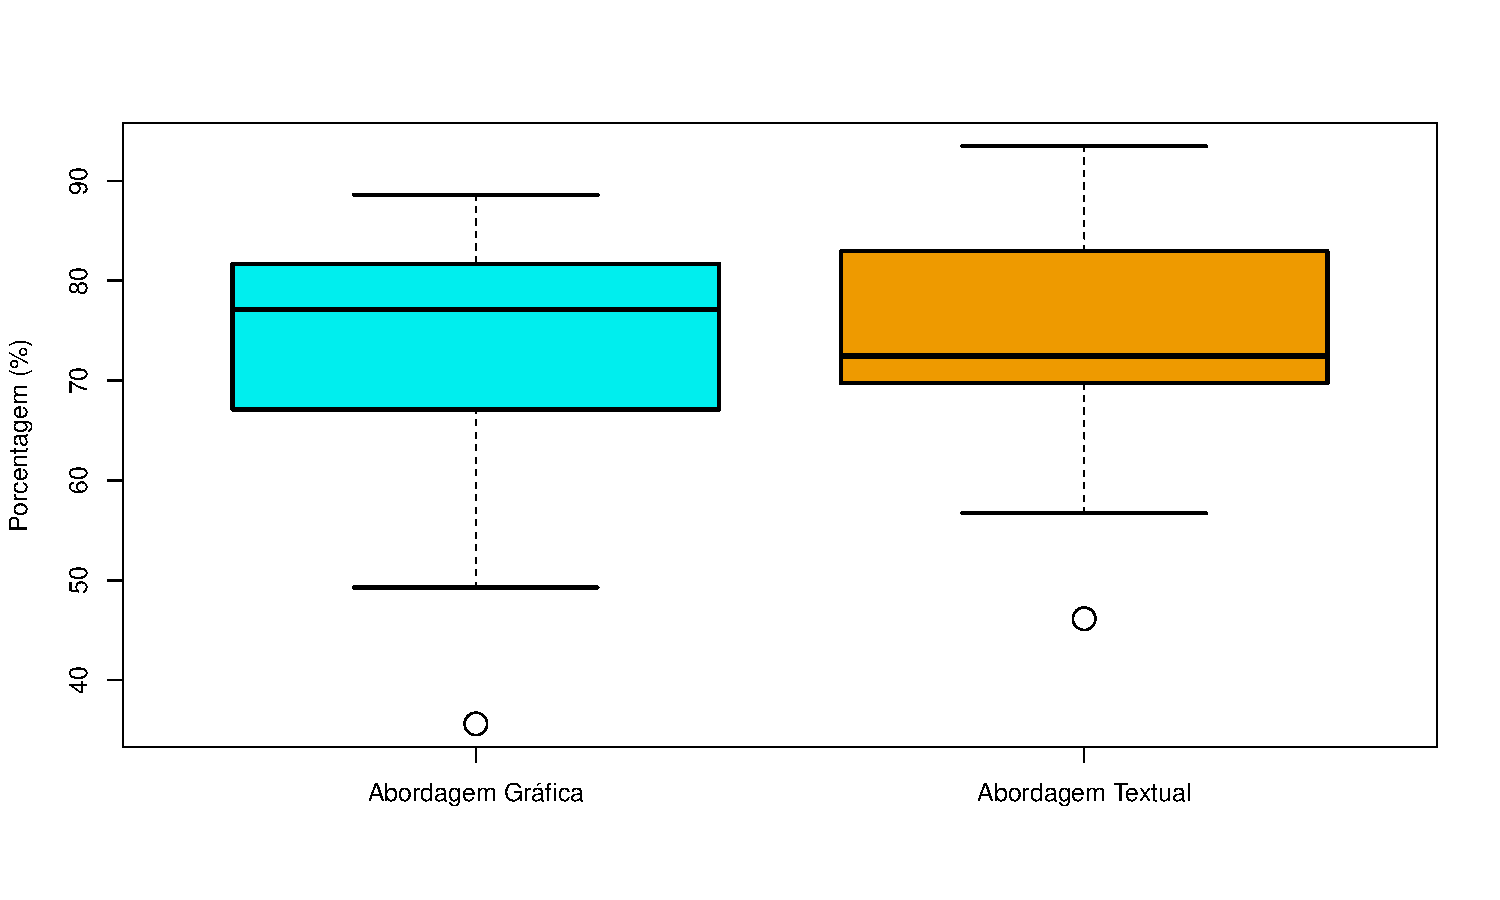
\includegraphics[width=0.8\textwidth]{ResultsExp/BoxPlotAcertos}
    \label{fig:BoxPlotMedidaF}
    \fonte{O autor.}
\end{figure}

% \begin{figure}[!htb]
%     \centering
%     \caption{Boxplot da \textit{Precisão} e \textit{Revocação} medidos nas abordagens.}
%     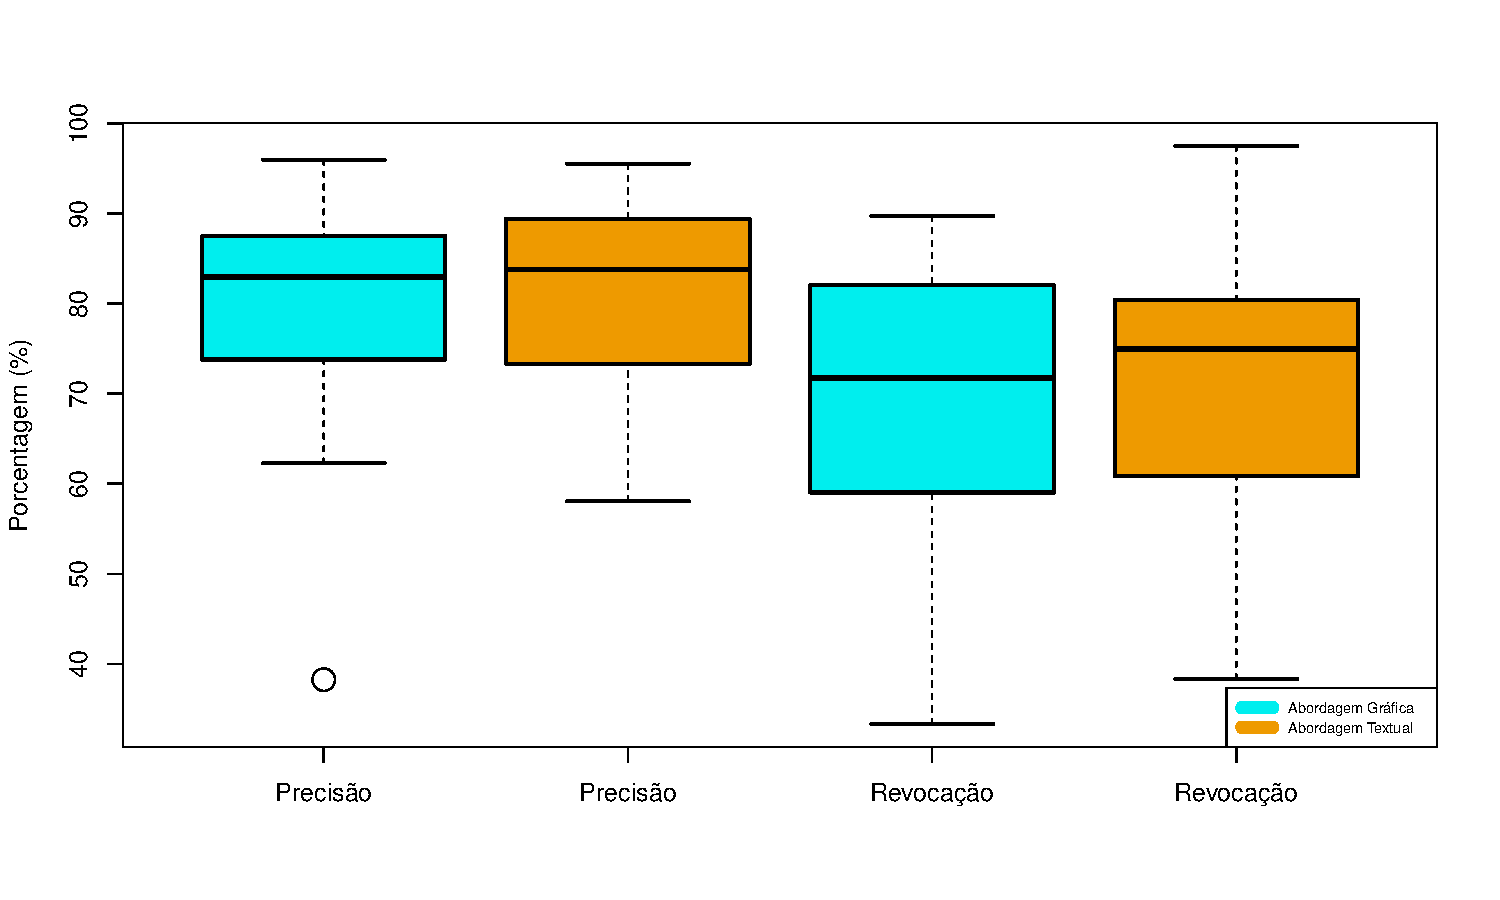
\includegraphics[width=0.7\textwidth]{ResultsExp/PrecisaoRevocacao}
%     \label{fig:BoxPlotPrecisaoRevocacao}
%     \fonte{O autor.}
% \end{figure}

\subsection{Avaliação Qualitativa}


A avaliação qualitativa se deu com a análise dos instrumentos aplicados após as tarefas de modelagem.
O primeiro destes, presente no Apêndice \ref{ap:Inst3Exp}, foi utilizado para responder a \ac{QP}3 referente a percepção de utilidade e facilidade de uso dos tratamentos.
Isto ocorreu mediante a seleção de atributos de qualidade descritos na ISO/IEC 25010.

Para tanto, foi estabelecido uma escala Likert de um (1) até seis (6).
Esta escala serviu para medir o nível de concordância dos sujeitos perante as afirmativas expostas no formulário.
Optou-se por um número par de alternativas para evitar possíveis respostas neutras.
Os sete (7) atributos de qualidade estão agrupados nas categorias de \textbf{Funcionalidade}, \textbf{Usabilidade} e \textbf{Qualidade em Uso}, sendo definidos a seguir.

\begin{itemize}
    
    \item \textbf{Funcionalidade} 
        \begin{itemize}
            \item \textit{Conformidade}: é capacidade do software de estar de acordo com normas, convenções e/ou prescrições similares relacionadas as funcionalidades.
        \end{itemize}
    
    \item \textbf{Usabilidade}
        \begin{itemize}
            \item \textit{Inteligibilidade}: é capacidade do software possibilitar ao usuário compreender se o software é apropriado e como ele pode ser usado para tarefas e condições de uso específicas;
            \item \textit{Apreensibilidade}: é a capacidade do software de possibilitar ao usuário aprender sua aplicação;
            \item \textit{Operacionalidade}: é a capacidade do software de possibilitar ao usuário operá-lo e controlá-lo.
        \end{itemize}
    
    \item \textbf{Qualidade em Uso}
        \begin{itemize}
            \item \textit{Qualidade em Uso}: é a capacidade do software de permitir que usuários atinjam metas especificadas com eficácia, produtividade, segurança e satisfação em contextos de uso especificados;
            \item \textit{Produtividade}: é a capacidade do software de permitir que seus usuários empreguem quantidade apropriada de recursos em relação à eficácia obtida, em um contexto de uso especificado;
            \item \textit{Satisfação}: é a capacidade do software de satisfazer usuários, em um contexto de uso específico.
        \end{itemize}
\end{itemize}

Após a sumarização dos resultados foi observada a boa aceitação por parte dos sujeitos para a ferramenta ERText, desenvolvida neste trabalho. 
A \autoref{fig:inst3GERALExp} sintetiza as respostas recebidas para cada item, evidenciando um certo grau de similaridade de percepção dos sujeitos durante a aplicação dos tratamentos.

\begin{figure}[!htb]
    \centering
    \caption{Avaliação dos atributos de qualidade dos tratamentos.}
    \label{fig:inst3GERALExp}
    \pgfplotsset{testbar/.style={
            xbar stacked,
            legend cell align=left,
            legend style={
                legend columns=6,
                font=\footnotesize,
                at={(xticklabel cs:1.0)},
                anchor=north east,
                draw=none
                },
            width=10cm,
            axis y line*= none, 
            axis x line*= bottom,
            xmajorgrids = false,
            xmin=0,xmax=27,
            ytick = data,
            yticklabels = {
                Conformidade  (ERText),
                Conformidade (BrModelo),
                Inteligibilidade (ERText),
                Inteligibilidade (BrModelo),
                Apreensibilidade (ERText),
                Apreensibilidade (BrModelo),
                Operacionalidade (ERText),
                Operacionalidade (BrModelo),
                Qualidade em uso (ERText),
                Qualidade em uso (BrModelo),
                Produtividade (ERText),
                Produtividade (BrModelo),
                Satisfabilidade (ERText),
                Satisfabilidade (BrModelo)
            },
            tick align = outside, xtick pos = left,
            bar width=7mm, y=10mm,
            enlarge y limits={abs=0.625},% 0.5 + 0.5*(y - bar width)/y [TeX.sx #47995]
            nodes near coords,
            nodes near coords align=center,%Move values in bar
            every node near coord/.append style={
                black,
                font=\footnotesize,
                text opacity=1,
                fill=white,
                fill opacity=0.7,
                outer sep=\pgflinewidth
            }
        }}
    \begin{tikzpicture}
    \begin{axis}[testbar] 
    \addplot[pattern color=red,pattern=north east lines] coordinates
        {(0,14)(0,13)(0,12)(0,11)(0,10)(0,9)(0,8)(2,7)(0,6)(0,5)(0,4)(1,3)(0,2)(1,1)};
    \addplot[pattern color=teal,pattern=vertical lines] coordinates
        {(0,14)(0,13)(0,12)(0,11)(0,10)(1,9)(0,8)(2,7)(0,6)(1,5)(0,4)(2,3)(0,2)(3,1)};
    \addplot[pattern color=gray, pattern=grid] coordinates
       {(1,14)(0,13)(0,12)(2,11)(2,10)(1,9)(0,8)(2,7)(0,6)(0,5)(2,4)(1,3)(1,2)(1,1)};
    \addplot[pattern color=magenta, pattern=north west lines] coordinates
       {(3,14)(2,13)(2,12)(1,11)(6,10)(4,9)(3,8)(5,7)(5,6)(2,5)(4,4)(6,3)(2,2)(6,1)};
    \addplot[pattern color=blue, pattern=horizontal lines] coordinates
       {(10,14)(3,13)(7,12)(4,11)(10,10)(16,9)(9,8)(8,7)(10,6)(7,5)(13,4)(10,3)(9,2)(7,1)};
    \addplot[pattern color=green, pattern=crosshatch dots] coordinates
       {(13,14)(22,13)(18,12)(20,11)(9,10)(5,9)(15,8)(8,7)(12,6)(17,5)(8,4)(7,3)(15,2)(9,1)};
    \legend{1-Discorda, 2, 3, 4, 5, 6-Concorda}
    \end{axis}
    \end{tikzpicture}
    
% \begin{tikzpicture}
% \begin{axis}[
%     xbar stacked,
%     legend cell align=center,
%     legend style={
%     legend columns=5,
%         at={(xticklabel cs:1.0)},
%         anchor=north east,
%         draw=none
%     },
%     ytick=data,
%     axis y line*=none,
%     axis x line*=bottom,
%     tick label style={font=\small},
%     legend style={font=\small},
%     label style={font=\small},
%     xtick={0,3,6},
%     xticklabel= {},
%     bar width=5mm,
%     ylabel={Questions},
%     yticklabels={P-Q1, T-Q1, P-Q2, T-Q2, P-Q3, T-Q3, P-Q4, T-Q4,P-Q5, T-Q5,P-Q6, T-Q6, P-Q7, T-Q7},
%     xmin=0,
%     xmax=6,
%     area legend,
%     y=6.5mm,
%     enlarge y limits={abs=0.625},
%     nodes near coords,
%     nodes near coords align=center,
%     every node near coord/.append style={
%         black,
%         font=\small,
%         text opacity=.65,
%         fill=white,
%         fill opacity=0.75,
%         outer sep=\pgflinewidth
%     }
% ]
% \addplot[pattern color=red,pattern=horizontal lines] coordinates
% {(0,14)(0,13)(0,12)(0,11) (3,10)(0,9)(0,8) (0,7) (0,6)(0,5)(0,4) (0,3) (0,2) (0,1)};   
% \addplot[pattern color=orange,pattern=grid] coordinates
% {(3,14) (0,13)(0,12)(0,11)(2,10) (1,9)(1,8)(0,7)(3,6)(0,5)(0,4)(3,3) (4,2) (0,1) };  
% \addplot[pattern color = green, pattern=crosshatch dots] coordinates
% {(0,14) (0,13) (3,12)(2,11)(1,10) (3,9)(4,8)(1,7)(3,6)(1,5)(3,4)(2,3)(2,2) (2,1) };   
% \addplot[pattern color=blue, pattern =vertical lines ] coordinates
% {(2,14) (3,13) (2,12)(3,11)(0,10)(2,9)(1,8)(4,7)(0,6)(3,5) (3,4)(1,3)(0,2)(4,1)};   
% \addplot[pattern color=gray, pattern = dots] coordinates
% {(1,14)(3,13)(1,12)(1,11)(0,10)(0,9)(0,8)(1,7) (0,6)(2,5) (0,4)(0,3)(0,2)(0,1) };   
% \legend{1-Disagree, 2, 3, 4, 5-Agree}

% \end{axis}
% \end{tikzpicture}
% \footnotesize
% T-Thoth answers; P-Parsifal answers;






% \begin{tikzpicture}
% \begin{axis}[
%     xbar stacked,
%     legend cell align=left,
%     legend style={
%     legend columns=2,
%         at={(xticklabel cs:1.0)},
%         anchor=north east,
%         draw=none
%     },
%     ytick=data,
%     axis y line*=none,
%     axis x line*=bottom,
%     tick label style={font=\scriptsize},
%     legend style={font=\scriptsize},
%     %legend style={font=\scriptsize,row sep=-0.1cm,/tikz/every odd column/.append style={column sep=0.01cm}},
%     label style={font=\scriptsize},
%     xtick={0,10,...,100},
%     width=\columnwidth,
%     bar width=3.5mm,
%     % xlabel={Frequencia em \%},
%     yticklabels={
%     {Q1 - OC},
%     {Q2 - TD},
%     {Q3 - OC},
%     {Q4 - TD},
%     {Q5 - OC},
%     {Q6 - TD},
%     {Q7 - OC},
%     {Q8 - TD},
%     {Q9 - OC},
%     {Q10 - TD},
%     {Q11 - OC},
%     {Q12 - TD}},
%     xmin=0,
%     xmax=100,
%     area legend,
%     y=5mm,
%     enlarge y limits={abs=0.625},
%     nodes near coords,
%     nodes near coords={\pgfmathprintnumber\pgfplotspointmeta\%},
%     nodes near coords align=center,%Move values in bar
%     every node near coord/.append style={
%         black,
%         font=\footnotesize,
%         text opacity=1,
%         fill=white,
%         fill opacity=0.7,
%         outer sep=\pgflinewidth
%     }
% ]
% \addplot[pattern color=blue,pattern=dots] coordinates
% {(0,0)(0,1)(0,2)(0,3)(0,4)(0,5)(0,6)(0,7)(0,8)(0,9)(0,10)(0,11)};
% \addplot[pattern color=red, pattern=vertical lines] coordinates
% {(4,0)(32,1)(0,2)(9,3)(13,4)(18,5)(0,6)(9,7)(5,8)(5,9)(0,10)(14,11)};
% \addplot[pattern color=cyan, pattern=grid] coordinates
% {(27,0)(9,1)(4,2)(5,3)(23,4)(27,5)(36,6)(23,7)(27,8)(41,9)(46,10)(45,11)};
% \addplot[pattern color=green, pattern=horizontal lines] coordinates
% {(55,0)(32,1)(55,2)(68,3)(41,4)(50,5)(46,6)(64,7)(64,8)(45,9)(36,10)(27,11)};
% \addplot[pattern color=orange, pattern=crosshatch dots] coordinates
% {(14,0)(27,1)(41,2)(18,3)(23,4)(5,5)(18,6)(4,7)(4,8)(9,9)(18,10)(14,11)};
% \legend{Strongly disagree,Disagree,Neither agree nor disagree,Agree,Strongly agree}; 

% \end{axis}  
% \end{tikzpicture}d
    \fonte{O autor.}
\end{figure}

% \begin{figure}[!htb]
%     \centering
%     \caption{Avaliação dos atributos de qualidade dos tratamentos.}
%     \label{fig:inst3GERALExp}
%      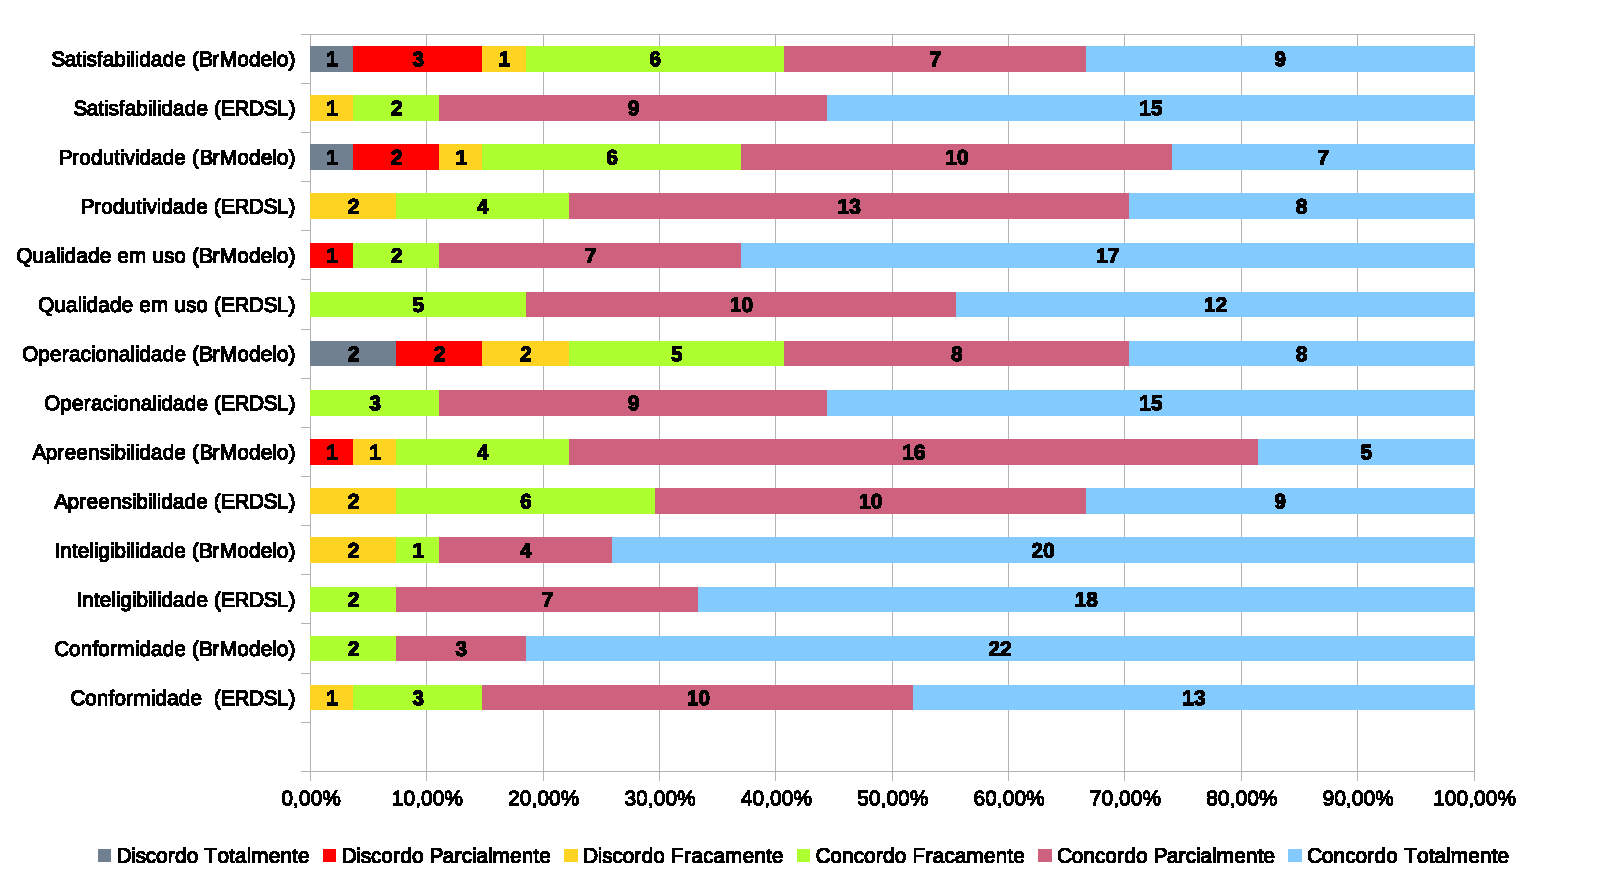
\includegraphics[width=1\textwidth]{img/EPS/Inst3GERAL.eps}
%     \fonte{O autor.}
% \end{figure}

Um ponto que pode ser ressaltado é o conjunto de respostas positivas em relação ao item \textit{Produtividade}, uma vez que no teste de hipótese relativo ao esforço o tratamento utilizando o BrModelo demonstrou uma menor necessidade de tempo para operação.
Na análise dos comentários abertos deste formulário de avaliação, que solicitavam que os participantes indicassem pontos positivos e negativos das ferramentas, foi relatado de forma explícita que a característica de autocomplemento de código proporcionou uma sensação de agilidade no processo de modelagem.

No que diz respeito a \ac{QP}4, sobre a avaliação dos construtores da \ac{DSL}, foram analisados os artefatos do instrumento presente no Apêndice \ref{ap:Inst4Exp}.
Este instrumento listava os oito (8) construtores de modelagem \ac{ER} cobertos pela \ac{DSL}, dispostos com uma escala Likert de um (1) até seis (6).
Novamente, optou-se pele número par na escala para evitar respostas neutras que poderiam levar a uma interpretação mais subjetiva.

Como pode ser observado na \autoref{fig:inst4GERALExp}, que compila todas as respostas recebidas, os construtores relacionados as Entidades e Atributos Descritivos foram os melhores avaliados, com todos os vinte sete (27) concordando com a sua atual representação.

Em contrapartida, todos os outros seis (6) obtiveram ao menos uma avaliação de discordância. 
Nesse sentido, destaca-se os contrutores dos \textit{Relacionamentos Ternários} e das Cardinalidades, com duas (2) e três (3) avaliações discordando das suas atuais representações respectivamente.

\begin{figure}[!htb]
    \centering
    \caption{Avaliação dos construtores da DSL.}
    \label{fig:inst4GERALExp}
    \pgfplotsset{testbar/.style={
            xbar stacked,
            legend cell align=left,
            legend style={
                legend columns=6,
                font=\footnotesize,
                at={(xticklabel cs:1.0)},
                anchor=north east,
                draw=none
                },
            width=10cm,
            axis y line*= none, 
            axis x line*= bottom,
            xmajorgrids = false,
            xmin=0,xmax=27,
            ytick = data,
            yticklabels = {Entidade, Atributo Referencial, Atributo Descritivo, Relação Binária, Relação Ternária, Autorelacionamento, Cardinalidade, Generalização},
            tick align = outside, xtick pos = left,
            bar width=7mm, y=10mm,
            enlarge y limits={abs=0.625},% 0.5 + 0.5*(y - bar width)/y [TeX.sx #47995]
            nodes near coords,
            nodes near coords align=center,%Move values in bar
            every node near coord/.append style={
                black,
                font=\footnotesize,
                text opacity=1,
                fill=white,
                fill opacity=0.5,
                outer sep=\pgflinewidth
            }
        }}
    \begin{tikzpicture}
    \begin{axis}[testbar] 
    \addplot[pattern color=red,pattern=north east lines] coordinates
        {(0,8) (0,7) (0,6) (0,5) (0,4) (0,3) (0,2) (0,1)};
    \addplot[pattern color=teal,pattern=vertical lines] coordinates
        {(0,8) (0,7) (0,6) (0,5) (0,4) (0,3) (0,2) (0,1)};   
    \addplot[pattern color=gray, pattern=grid] coordinates
        {(0,8) (1,7) (0,6) (1,5) (2,4) (1,3) (3,2) (1,1)};   
    \addplot[pattern color=magenta, pattern=north west lines] coordinates
        {(1,8) (2,7) (4,6) (3,5) (9,4) (5,3) (2,2) (2,1)};   
    \addplot[pattern color=blue, pattern=horizontal lines] coordinates
        {(5,8) (6,7) (6,6) (7,5) (7,4) (9,3) (7,2) (7,1)};   
    \addplot[pattern color=green, pattern=crosshatch dots] coordinates
        {(21,8) (18,7) (17,6) (16,5) (9,4) (12,3) (15,2) (17,1)};  
    \legend{1-Discorda, 2, 3, 4, 5, 6-Concorda}
    \end{axis}
    \end{tikzpicture}




% \begin{figure}[!ht]
% \centering
% \caption{Resultados do formulários de avaliação.}
% \begin{tikzpicture}
% \begin{axis}[
%     xbar stacked,
%     legend cell align=center,
%     legend style={
%     legend columns=5,
%         at={(xticklabel cs:1.0)},
%         anchor=north east,
%         draw=none
%     },
%     ytick=data,
%     axis y line*=none,
%     axis x line*=bottom,
%     tick label style={font=\small},
%     legend style={font=\small},
%     label style={font=\small},
%     xtick={0,5,10},
%     xticklabel= {},
%     bar width=7mm,
%     ylabel={Formulário/Grupo},
%     yticklabels={F1-C, F1-E, F2-C, F2-E, F3-C, F3-E},
%     xmin=0,
%     xmax=10,
%     area legend,
%     y=9mm,
%     enlarge y limits={abs=0.825},
%     nodes near coords,
%     nodes near coords align=center,
%     every node near coord/.append style={
%         black,
%         font=\small,
%         text opacity=.65,
%         fill=white,
%         fill opacity=0.6,
%         outer sep=\pgflinewidth
%     }
% ]
% %NOTA 1
% \addplot[pattern color=red,pattern=horizontal lines] coordinates
% {(0,6)(0,5)(0,4)(0,3)(0,2)(0,1)};
% %NOTA 2
% \addplot[pattern color=orange,pattern=grid] coordinates
% {(1,6)(1,5)(1,4)(0,3)(1,2)(0,1)};   
% \addplot[pattern color = green, pattern=crosshatch dots] coordinates
% % NOTA 3
% {(3,6)(3,5)(5,4)(2,3)(5,2)(1,1)};   
% \addplot[pattern color=blue, pattern =vertical lines ] coordinates
% %NOTA 4
% {(2,6)(3,5)(1,4)(4,3)(3,2)(3,1)};   
% \addplot[pattern color=gray, pattern = dots] coordinates
% %NOTA 5
% {(3,6)(3,5)(2,4)(4,3)(0,2)(6,1)};   
% \legend{1-Disagree, 2, 3, 4, 5-Agree}

% \end{axis}
% \end{tikzpicture}
% \footnotesize
% \label{img:respostas1}
% 	\fonte{O autor.}
% \end{figure}
    \fonte{O autor.}
\end{figure}

% \begin{figure}[!htb]
%     \centering
%     \caption{Avaliação dos construtores da \ac{DSL}.}
%     \label{fig:inst4GERALExp}
%     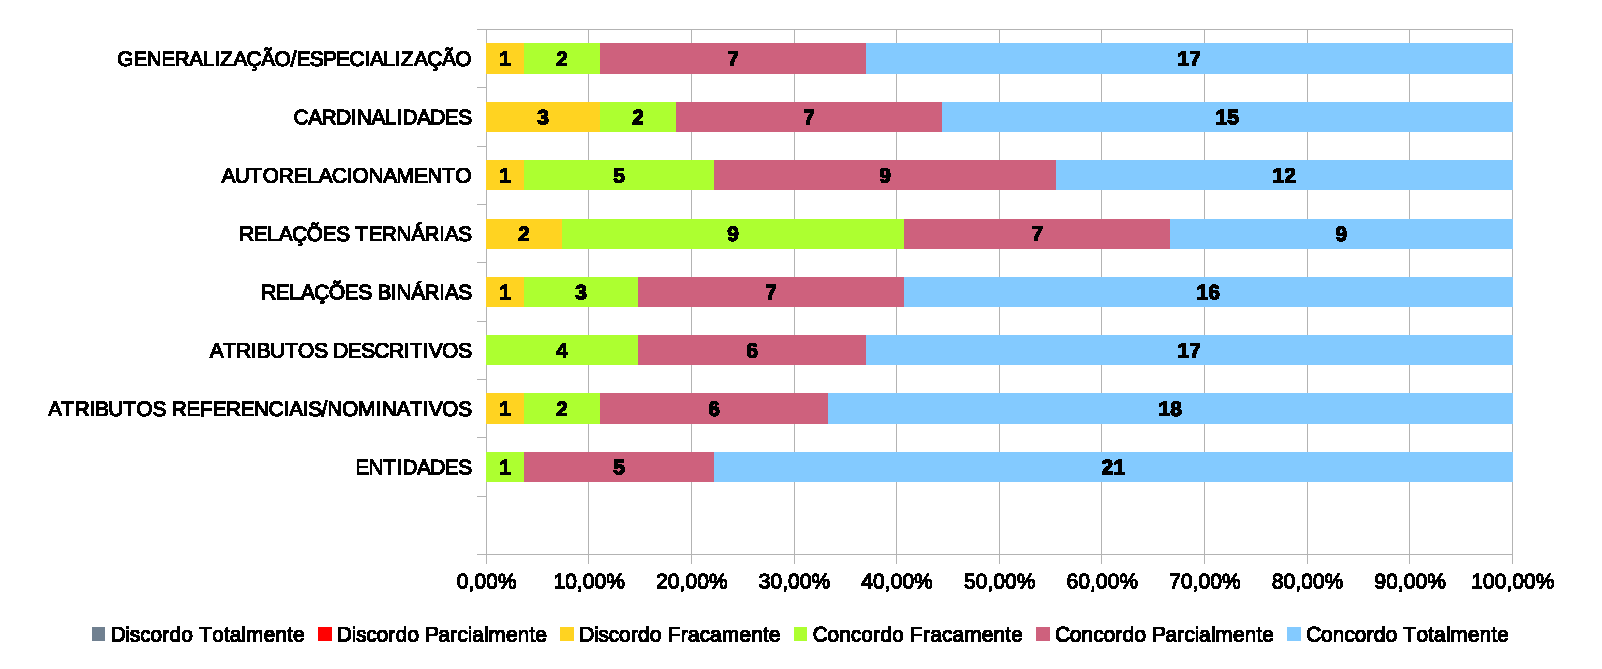
\includegraphics[width=1\textwidth]{img/EPS/Inst4GERAL.eps}
%     \fonte{O autor.}
% \end{figure}

\section{Lições do Capítulo} \label{sec:licoesExp}


Neste capítulo foi apresentado o protocolo e a execução do experimento controlado que foi conduzido para avaliação da proposta deste trabalho.
Para tanto, foram observados fatores como esforço, efetividade, utilidade e facilidade de uso.

Com as respostas obtidas foi possível responder as quatro (4) \acp{QP} do experimento, bem como as duas (2) hipóteses associadas.
A partir da análise feita é possível destacar os seguintes temas:
\begin{itemize}
    \item \textit{Esforço}: a abordagem gráfica para modelagem \ac{ER} mostrou necessitar de menos esforço associado para realizar as tarefas solicitadas, porém considera-se que essa diferença pode ser diminuída com melhorias futuras na ERText;
    \item \textit{Efetividade}: não foi identificado uma diferença média que justifique afirmar que uma abordagem foi melhor do que a outra no que diz respeito a efetividade, entretanto observa-se que existe a necessidade de serem realizados testes que envolvam problemas de complexidades maiores para uma melhor avaliação.
    \item \textit{Comparação qualitativa entre os tratamentos}: foi possível observar que há certo equilíbrio entre os tratamentos, mas destaca-se a avaliação positiva que o atributo \textit{Produtividade} da ERText recebeu dos participantes do experimento. 
    Em razão de ter sido a primeira vez que os sujeitos tiveram contato com a gramática, bem como da ferramenta estar em sua primeira versão, este é um ponto que chama a atenção e merece destaque;
    \item \textit{Avaliação da linguagem proposta}: em decorrência da avaliação dos construtores da \ac{DSL} proposta, existem algumas lacunas quanto ao \textit{design} da linguagem que precisam ser revistos, em especial atenção as cardinalidades e relacionamentos ternários implementados.
    Uma vez que está previsto o prosseguimento do desenvolvimento da linguagem, a execução de uma possível refatoração, e também a implementação de novos construtores, se mostra um passo natural para sua evolução.
\end{itemize}



A partir dos resultados é possível concluir que existe viabilidade para o uso da abordagem textual para modelagem \ac{ER}, uma vez que os resultados não obtiveram diferenças severas no que diz respeito as atividades executadas.
Contudo, com as respostas alcançadas neste experimento verifica-se a necessidade da realização de melhorias, tanto na implementação da ERText quanto no planejamento e execução de um novo experimento controlado.


%#################################################################
\chapter{Considerações Finais}\label{consideracoesFinais}
%#################################################################

\textcolor{red}{\textbf{REESCREVER TUDO}}

% Este trabalho abordou o projeto de conclusão de curso expondo seu planejamento metodológico, a fundamentação teórica, um mapeamento multivocal de literatura e a proposta de uma \ac{DSL} textual para modelagem conceitual de \acp{BD}.

% Como principais resultados obtidos está a investigação conduzida para compreender o estado da arte e da prática no uso de \acp{DSL} para modelagem de \acp{BD}, bem como a criação de uma \ac{DSL} textual utilizando o \textit{framework} Xtext, ferramenta \textit{open source} que permitiu a integração do protótipo a um \ac{RCP} Eclipse. 

% Outro ponto que merece destaque foi o esforço dos pesquisadores envolvidos neste estudo para a realização de dois artigos, sendo um abordando o \ac{SLM} e submetido ao \textit{ER - International Conference on Conceptual Modeling} (ER'2019), e outro abrangendo toda o \ac{MLM}, o qual foi submetido ao Simpósio Brasileiro de Bancos de Dados (SBBD'2019). Ambos os trabalhos estão em fase de avaliação.

% Pretende-se que ao final do trabalho esta proposta não apenas realize modelagem, mas também a transformação dos modelos \ac{ER} gerados em \textit{scripts} \ac{SQL} para diferentes tecnologias \acp{SGBD}, \textit{e.g.} PostgreSQL, MySQL e SQL Server.

%#################################################################
\section{Trabalhos Futuros}
%#################################################################

\textcolor{red}{\textbf{REESCREVER TUDO}}

% Na fase atual desta pesquisa pode-se dizer que foram obtidos avanços, porém ainda é necessário realizar a finalização de diversos aspectos da proposta. 
% Os principais pontos que devem ser investigados e desenvolvidos dizem respeito à transformação completa dos modelos conceituais para modelos lógicos, bem como a geração de \textit{scripts} \ac{SQL} que representem o modelo físico.

% Pretende-se resolver estas questões com o andamento do trabalho e, com isto feito, realizar uma avaliação experimental da proposta. 
% É importante salientar que a \ac{DSL} será avaliada preliminarmente ainda no começo do \ac{TCC} II, visando assim obter o refinamento da gramática da linguagem criada.

% %#################################################################
% \section{Cronograma}
% %#################################################################

% Para o restante da execução da pesquisa, o desenvolvimento deste trabalho se dará conforme as atividades descritas na \autoref{tbl:cronograma}.


% \begin{landscape}
% \definecolor{midgray}{gray}{.5}
% \begin{table}[!htb]
%     \caption{Cronograma do Trabalho de Conclusão de Curso.}
%     \label{tbl:cronograma}
% 	\centering
% 		\begin{tabular}{l|c|c|c|c|c|c|c|c|c}
% 		\bottomrule
% 		\rowcolor[HTML]{C0C0C0}
% 		\textbf{ATIVIDADE}&\multicolumn{5}{c|}{\large\textbf{2019/1}}&\multicolumn{4}{c}{\large\textbf{2019/2}}\\
% 		\hline
% 		\rowcolor[HTML]{C0C0C0}
% 		&\textbf{MAR}&\textbf{ABR}&\textbf{MAI}&\textbf{JUN}&\textbf{JUL}&\textbf{AGO}&\textbf{SET}&\textbf{OUT}&\textbf{NOV}\\
% 		\hline
% 		Elaboração da proposta de TCC &\cellcolor{Blue}&&&&&&&&\\
% 		\hline
% 		Pesquisa bibliográfica da fundamentação teórica &\cellcolor{Blue}&\cellcolor{Blue}&\cellcolor{Blue}&&&&&&\\
% 		\hline
% 		Planejamento e execução do MLM &\cellcolor{Blue}&\cellcolor{Blue}&\cellcolor{Blue}&&&&&&\\
% 		\hline	
% 		Análise de qualidade dos Resultados do MLM &&\cellcolor{Blue}&\cellcolor{Blue}&&&&&&\\
% 		\hline			
% 		Extração e análise dos dados do MLM &&\cellcolor{Blue}&\cellcolor{Blue}&&&&&&\\
% 		\hline	
% 		Implementação do protótipo &&&\cellcolor{Blue}&\cellcolor{Blue}&&&&&\\
% 		\hline
% 		Demonstração do protótipo &&&&\cellcolor{Blue}&&&&&\\
% 		\hline
% 		Escrita do TCC I &&\cellcolor{Blue}&\cellcolor{Blue}&\cellcolor{Blue}&&&&&\\
% 		\hline
% 		Aplicação das melhorias sugeridas pela banca de TCC1&&&&\cellcolor{midgray}&\cellcolor{midgray}&&&&\\
% 		\hline
% 		Planejamento da avaliação preliminar &&&&\cellcolor{midgray}&\cellcolor{midgray}&&&&\\
% 		\hline
% 		Execução da avaliação preliminar &&&&&\cellcolor{midgray}&&&&\\
% 		\hline	
% 		Análise da avaliação preliminar &&&&&\cellcolor{midgray}&\cellcolor{midgray}&&&\\
% 		\hline	
% 		Evolução do desenvolvimento &&&&&\cellcolor{midgray}&\cellcolor{midgray}&\cellcolor{midgray}&\cellcolor{midgray}&\\
% 		\hline	
% 		Planejamento da avaliação experimental &&&&&&\cellcolor{midgray}&\cellcolor{midgray}&&\\
% 		\hline	
% 		Execução da avaliação experimental &&&&&&&\cellcolor{midgray}&&\\
% 		\hline	
% 		Análise dos resultados da avaliação experimental &&&&&&&\cellcolor{midgray}&\cellcolor{midgray}&\\
% 		\hline	
% 		Escrita de artigos para submissão em eventos científicos
% 		&&&&&\cellcolor{midgray}&\cellcolor{midgray}&\cellcolor{midgray}&\cellcolor{midgray}&\cellcolor{midgray}\\
% 		\hline	
% 		Escrita do TCC II 
% 		&&&&&&\cellcolor{midgray}&\cellcolor{midgray}&\cellcolor{midgray}&\cellcolor{midgray}\\
% 		\toprule	
% 		\end{tabular}
% 		\fonte{O autor.}
% \end{table}
% \end{landscape}




%%==============================================================================
\chapter{Desenvolvimento}\label{desenvolvimento}
%==============================================================================

Alguns cuidados devem ser tomados no uso deste pacote. Leia as orientações a seguir e contate o responsável em caso de dúvidas.


%------------------------------------------------------------------------------
\section{Formatação}
%------------------------------------------------------------------------------

Embora não faça diferença no resultado final, é importante formatar adequadamente o seu código \LaTeX.
  Da mesma forma que para outras linguagens de programação, isso aumenta a legibilidade do código e ajuda a encontrar partes específicas mais rapidamente.
  As principais dicas para arquivos \TeX são:
 \begin{itemize}
   \item Indente seu código. Não só os ambientes (begin, end) mas também os parágrafos! Coloque cada sentença em uma linha, indentando a partir da segunda;
   \item Coloque marcações comentadas para delimitar o início de capítulos, seções, etc. Isso facilita buscar partes específicas em um arquivo.
 \end{itemize}

Cuidado com abreviaturas e acrônimos.
  É fácil esquecer de os definir ou definir de maneira diferente em capítulos diferentes.
  Use os comandos do pacote \texttt{acro} para abreviaturas e acrônimos.
  Por exemplo, \ac{fig} é uma abreviação, então \ac{tcc} é um acrônimo/sigla.
  Eles são definidos no preâmbulo do documento.

Também vale a pena usar uma tabela de nomenclatura caso você use muitos símbolos, em especial símbolos matemáticos.
  Veja os comandos do pacote \texttt{nomencl}.
  As definições também ficam no preâmbulo do documento.


%------------------------------------------------------------------------------
\section{Codificação dos arquivos: UTF8}
%------------------------------------------------------------------------------

A codificação de todos os arquivos deste pacote é \texttt{UTF8}.
  É necessário que você utilize a mesma codificação nos documentos que escrever, inclusive nos arquivos de bases bibliográficas |.bib|.


%------------------------------------------------------------------------------
\section{Citações}
%------------------------------------------------------------------------------

\index{citações!diretas}Utilize o ambiente \texttt{citacao} para incluir citações diretas com mais de três linhas:

\begin{citacao}
As citações diretas, no texto, com mais de três linhas, devem ser destacadas com recuo de 4 cm da margem esquerda, com letra menor que a do texto utilizado e sem as aspas.
  No caso de documentos datilografados, deve-se observar apenas o recuo \cite[5.3]{NBR10520:2002}
\end{citacao}

\index{citações!simples}Citações simples, com até três linhas, devem ser incluídas com aspas.
  Observe que em \LaTeX~as aspas iniciais são diferentes das finais: ``Amor é fogo que arde sem se ver''.

Para as citações indiretas, o comando padrão, \verb|\cite|, realiza a forma mais comum de citação \cite{SisbiUnipampa2011}.
  A outra das formas mais usadas, para citar em texto corrido, é conseguida com o comando \verb|\citeonline|: segundo \citeonline{SisbiUnipampa2011}, na citação indireta, o número da página é opcional.


%------------------------------------------------------------------------------
\subsection{Referências internas}\label{sec:referencias_internas}
%------------------------------------------------------------------------------

Usa-se o comando \verb|\ref{}| para referenciar uma Tabela ou Figura.
  Por exemplo, esta é uma referência para a Tabela~\ref{tab:nivinv}.
  Mas também pode-se usar o comando \verb|\autoref{}|, que insere o tipo também.
  Por exemplo, esta é outra referência para a \autoref{tab:nivinv}.

Há vários outros comandos interessantes.
  Eles estão no fonte do \autoref{introducao}, na \autoref{sec:referencias_internas}
  \footnote{O número do capítulo indicado é \ref{introducao}, que se inicia à página \pageref{introducao}.}
  (\nameref{introducao}, \autopageref{introducao}).


%------------------------------------------------------------------------------
\section{Tabelas}
%------------------------------------------------------------------------------

\index{tabelas}A \autoref{tab:nivinv} é um exemplo de tabela construída em \LaTeX.
  Como sugestão de formatação, evite ao máximo o uso de linhas verticais.
  As colunas de uma tabela devem ser separadas visivelmente.
  O contrário indica que a tabela está mal formatada ou que certas informações não deveriam estar nela.

Da mesma forma, evite o uso de linhas horizontais para separar linhas da tabela.
  Use-as apenas para separar o cabeçalho e eventuais partes importantes.
  Para obter um resultado ainda mais elegante, use os comandos do pacote \texttt{booktabs}.

Veja essas sugestões aplicas na \autoref{tab:nivinv}.

\begin{table}[!htb]
\footnotesize
\caption[Níveis de investigação]{Níveis de investigação.}
\label{tab:nivinv}
\begin{tabular}{m{2.6cm}m{6.0cm}m{2.25cm}m{3.40cm}}
  \toprule
  \textbf{Nível de Investigação} & \textbf{Insumos}  & \textbf{Sistemas de Investigação}  & \textbf{Produtos}  \\
  \midrule
  Meta-nível & Filosofia\index{filosofia} da Ciência  & Epistemologia & Paradigma  \\
  Nível do objeto & Paradigmas do metanível e evidências do nível inferior & Ciência  & Teorias e modelos \\
  Nível inferior & Modelos e métodos do nível do objeto e problemas do nível inferior & Prática & Solução de problemas  \\
  \bottomrule
\end{tabular}
\fonte{\citeonline{van86}}
\end{table}


Uma opção avançada para a criação de tabelas é usar o pacote \texttt{pgfplotstable}.
  Ele permite que os dados de um arquivo sejam lidos e colocados em uma tabela, formatando-os da maneira que se quiser.
  A \autoref{tab:dados} é um exemplo.
  Veja o arquivo \texttt{desenvolvimento.tex} para os comandos necessários.

% Necessário o pacote filecontents
% Especifica o conteúdo que será gravado no dado arquivo (nesse caso, resultados.txt)
\begin{filecontents*}{resultados.txt}
tamanho metodo1 metodo2 metodo3
10  30    36.2  28.3
20  54.8  52.5  56.8
30  65    59.6  74.1
40  64.5  59.6  76.7
50  64.6  59.6  76.5
\end{filecontents*}

% Para definir os estilos das colunas e da tabela
\pgfplotstableset{
     %columns={tamanho,metodo1,{grad(log(metodo2),log(metodo3))}},
     columns/metodo1/.style={
         column name=\textsc{Método 1 (\%)},
         column type=c,
         %dec sep align={c},
         %sci,sci zerofill,sci subscript,
         fixed,fixed zerofill,
         precision=1},
     columns/metodo2/.style={
         column name=\textsc{Método 2 (\%)},
         column type=c,
         fixed,fixed zerofill,precision=1},
     columns/metodo3/.style={
         column name=\textsc{Método 3 (\%)},
         fixed,fixed zerofill,precision=1},
     columns/media/.style={
         column name=\textsc{Média (\%)},
         fixed,fixed zerofill,precision=1},
     create on use/media/.style={
         create col/expr={(\thisrow{metodo1}+\thisrow{metodo2}+\thisrow{metodo3})/3}},
     every head row/.style={
         before row=\toprule,after row=\midrule},
     every last row/.style={
         after row=\bottomrule}}

\begin{table}[!phtb]
  \caption{Exemplo de tabela com dados de arquivo.}
  \label{tab:dados}
  \begin{center}
    % Lê do arquivo resultados.txt as colunas especificadas e as formata de acordo com
    % os estilos acima ou com os estilos especificados aqui (nesse caso, para a coluna tamanho).
    \pgfplotstabletypesetfile[
      columns={tamanho,metodo1,metodo2,metodo3,media},
      columns/tamanho/.style={column name=\textsc{Tamanho}}
    ]{resultados.txt}
  \end{center}
\end{table}


%------------------------------------------------------------------------------
\section{Figuras}
%------------------------------------------------------------------------------

\index{figuras}Figuras podem ser criadas diretamente em \LaTeX.
  Uma das melhores formas, por ser relativamente simples, bem documentada e gerar ótimos resultados, é com o uso do pacote tikz\footnote{Há vários exemplos em \url{http://www.texample.net/}.}.
  Ele permite gerar diagramas, árvores, fluxogramas etc.
  A \autoref{fig:fib} mostra um exemplo simples de árvore.

\begin{figure}[!htb]
  \caption{Árvore de recursão de Fibonacci.}\label{fig:fib}
  \begin{center}
  \begin{tikzpicture}[level/.style={sibling distance=160mm/(2^#1)},
                      level 4/.style={sibling distance=18mm},
                      every node/.style={minimum width=5mm}]
    \node [circle,draw] (z) {$fib(5)$}
      child {node [circle,draw] (a) {$fib(4)$}
        child {node [circle,draw] (b) {$fib(3)$}
          child {node [circle,draw=red] (c) {$fib(2)$}
            child {node [circle,draw] (d) {$fib(1)$}}
            child {node [circle,draw] (e) {$fib(0)$}}
          }
          child {node [circle,draw] (f) {$fib(1)$}}
        }
        child {node [circle,draw=red] (g) {$fib(2)$}
          child {node [circle,draw] (h) {$fib(1)$}}
          child {node [circle,draw] (i) {$fib(0)$}}
        }
      }
      child {node [circle,draw] (j) {$fib(3)$}
        child {node [circle,draw=red] (k) {$fib(2)$}
          child {node [circle,draw] (l) {$fib(1)$}}
          child {node [circle,draw] (m) {$fib(0)$}}
        }
        child {node [circle,draw] (n) {$fib(1)$}}
      };
  \end{tikzpicture}
  \end{center}
\end{figure}

Junto com o pacote pgfplots também é possível gerar gráficos de funções ou a partir de dados em um arquivo (como no caso da \autoref{tab:dados}).
  As Figuras \ref{fig:grafico1} e \ref{fig:grafico2} mostram exemplos de gráficos de função, e a \autoref{fig:grafico_dados} um exemplo de gráfico a partir dos mesmos dados que os da \autoref{tab:dados}.

\begin{figure}[!htb]
  \caption{Gráfico produzido diretamente no arquivo fonte.}\label{fig:grafico1}
  \begin{center}
  \begin{tikzpicture}[scale=1]
  \begin{axis}[
      width=.65\textwidth,
      ymin=0,xmin=0,xmax=1000,
      xlabel=$n$,ylabel=$T(n)$,
      ylabel near ticks,
      scaled ticks=false, % Evita o uso de notação exponencial 10^2
      ticklabel style={/pgf/number format/.cd,fixed,use comma,1000 sep={}}, % Para vírgula como separador decimal
      legend pos=outer north east,
      legend style={draw=none},
    ]
    \addplot[blue,thick,domain=1:1000] {1 * x * ln(x) / ln(2)} node[near end,above] {$g(n)$};
    \addplot[green,thick,domain=1:1000] {12 * x * ln(x) / ln(2)} node[near end,above left] (g) {$12g(n)$};
    \addplot[orange,thick,domain=1:1000] {5 * x * ln(x) / ln(2) + 21000} node[near end,above] {$f(n)$};
    \addplot+[red,very thick,dashed,mark=o,const plot,samples at=354] {12 * x * ln(x) / ln(2)};
    \addplot[red,thick,dashed,const plot] coordinates {(354,0) (354,35970)};
    %\addlegendentry{$g(n)$}; %{$n \lg(n)$}
    %\addlegendentry{$12g(n)$}; %{$12n \lg(n)$}
    %\addlegendentry{$f(n)$};
    \draw[black!70,very thin,solid,text=black] (axis cs:354,35970) -- (axis cs:250,50000) node[above] {$n_0\approx 354$};
    \draw[black!70,very thin,solid,text=black] (g.west) -> (axis cs:400,90000) node[below] {$c=12$};
  \end{axis}
  \end{tikzpicture}
  \end{center}
\end{figure}

\begin{figure}[!htb]
  \caption{Outro gráfico feito em \LaTeX.}
  \label{fig:grafico2}
  \begin{center}
  \begin{tikzpicture}
  \begin{axis}[
      width=.8\textwidth,
      ymin=0,xmin=0,xmax=150,
      xlabel=$n$,ylabel=$T(n)$,
      ylabel near ticks,
      scaled ticks=false, % Evita o uso de notação exponencial 10^2
      yticklabel style={/pgf/number format/.cd,fixed,use comma,1000 sep={}}, % Para vírgula como separador decimal
      legend pos=north west,
      legend style={draw=none},
    ]
    \addplot[blue,mark=*,thick,domain=1:150] {6 * x * ln(x) / ln(2) + 6 * x};
    \addplot[orange,mark=square,thick,domain=1:150] {1 / 2 * x^2};
    \addlegendentry{$6n \lg(n) + 6n$}
    \addlegendentry{$\frac{1}{2}n^2$}
  \end{axis}
  \end{tikzpicture}
  \end{center}
\end{figure}


\begin{figure}[!htb]
  \caption{Variação dos resultados utilizando seleção por Janela Deslizante.}
  \label{fig:grafico_dados}
  \begin{center}
  \begin{tikzpicture}[scale=1]
    \begin{axis}[
      width=0.9\textwidth,%height=0.6\textwidth,
      xmode=normal,ymode=normal,
      ymin=20,
      xtick=data,%ticks=both,
      xlabel=Tamanho,
      ylabel=Acerto (\%),
      legend pos=south east,
      %legend style={draw=none},
    ]
    \addplot+[thick] table [x=tamanho,y=metodo1,header=true] {resultados.txt};
    \addlegendentry{Método 1}
    \addplot+[thick,mark=square] table [x=tamanho,y=metodo2,header=true] {resultados.txt};
    \addlegendentry{Método 2}
    \addplot+[thick,mark=triangle] table [x=tamanho,y=metodo3,header=true] {resultados.txt};
    \addlegendentry{Método 3}
  \end{axis}
  \end{tikzpicture}
\end{center}
\end{figure}


Figuras também podem ser incorporadas de arquivos externos, como é o caso da \autoref{fig:grafico_excel}.
  Se a figura que ser incluída se tratar de um diagrama, um gráfico ou uma ilustração que você mesmo produza, priorize o uso de imagens vetoriais no formato PDF.
  Com isso, o tamanho do arquivo final do trabalho será menor, e as imagens terão uma apresentação melhor, principalmente quando impressas, uma vez que imagens vetorias são perfeitamente escaláveis para qualquer dimensão.
  Nesse caso, se for utilizar o Microsoft Excel para produzir gráficos, ou o Microsoft Word para produzir ilustrações, exporte-os como PDF e os incorpore ao documento conforme o exemplo abaixo.
  No entanto, para manter a coerência no uso de software livre (já que você está usando \LaTeX e \abnTeX), teste a ferramenta \textsf{InkScape}\index{InkScape}\footnote{\url{http://inkscape.org/}}.
  Ela é uma excelente opção de código-livre para produzir ilustrações vetoriais, similar ao CorelDraw\index{CorelDraw} ou ao Adobe Illustrator\index{Adobe Illustrator}.

De todo modo, caso não seja possível utilizar arquivos de imagens como PDF, utilize qualquer outro formato, como PNG, JPEG, etc.
  Nesse caso, você pode tentar aprimorar as imagens incorporadas com o software livre \textsf{Gimp}\index{Gimp}\footnote{\url{http://www.gimp.org/}}.
  Ele é uma alternativa livre ao Adobe Photoshop\index{Adobe Photoshop}.

\begin{figure}[htb]
  \caption{Gráfico produzido em Excel e salvo como PDF.}\label{fig:grafico_excel}
  \begin{center}
      \includegraphics[scale=0.5]{img/abntex2-modelo-img-grafico}
  \end{center}
  \fonte{\citeonline[p. 24]{araujo2012}}
\end{figure}


A \autoref{fig:exemplo} na página \pageref{fig:exemplo} contém duas subfiguras, \autoref{subfig:exemplo:arquivo} e \subcaptionref{subfig:exemplo:tikz}.
  A \autoref{subfig:exemplo:arquivo} foi inserida de um arquivo externo, enquanto a \autoref{subfig:exemplo:tikz} foi escrita dentro do próprio código \TeX.
  A \autoref{fig:exemplo2} contém o mesmo exemplo, mas usando comandos diferentes para inserir as Subfiguras \ref{subfig:exemplo2:arquivo} e \subcaptionref{subfig:exemplo2:tikz}.

\begin{figure}[!htb]
  \centering
  \caption{Exemplo de subfiguras.}\label{fig:exemplo}
  \subbottom[Uma figura de um arquivo.]{\includegraphics[scale=1]{img/exemplo}\label{subfig:exemplo:arquivo}}\fonte{\citeonline{Moro2012}}
  \qquad
  \subbottom[Uma figura em puro código TikZ.]{%
    \begin{tikzpicture}
      [tipo1/.style={rectangle,draw,minimum height=13mm,minimum width=9mm},
       tipo2/.style={circle,draw,minimum height=6mm,minimum width=6mm,
                     prefix after command={\pgfextra{\tikzset{every label/.style={font=\footnotesize}}}}},
       tiposeta/.style={->,shorten >=6pt,shorten <=6pt,>=triangle 60,thick}]
      \node [tipo1] (base) [label=below:Base Station] {};
      \node [tipo1] (sink) [right=22mm of base,label=below:Nodo Sink] {};
      \node [tipo2] (sensor1) [above right=4mm and 17mm of sink,label=right:Sensor] {};
      \node [tipo2] (sensor2) [right=22mm of sink,label=right:Sensor] {};
      \node [tipo2] (sensor3) [below right=4mm and 17mm of sink,label=right:Sensor] {};
      \draw [tiposeta] (base.east) -- (sink.west);
      \draw [tiposeta] (sink.east) -- (sensor1.south west);
      \draw [tiposeta] (sink.east) -- (sensor2.west);
      \draw [tiposeta] (sink.east) -- (sensor3.north west);
    \end{tikzpicture}
    \label{subfig:exemplo:tikz}%
  }
  \legend{Alterado: de \citeonline{Moro2012}}%
\end{figure}

Na \autoref{fig:exemplo}, as legendas (que indicam a fonte) para cada subfigura só funcionaram porque as figuras ficaram uma embaixo da outra.
  Se elas estivessem lado a lado, a inserção do comando \verb|\legend| em cada uma faria com que elas ficassem organizadas na vertical.
  Uma legenda geral funcionaria, entretanto.

Na \autoref{fig:exemplo2}, tanto legendas para subfiguras quanto uma legenda geral funcionam.

\begin{figure}[!htb]
  \centering
  \caption{Mesmo exemplo de subfiguras, agora em escala.}\label{fig:exemplo2}
  \begin{minipage}{0.48\textwidth}
    \centering
    \includegraphics[scale=.5]{img/exemplo}
    \subcaption{Uma figura de um arquivo.\label{subfig:exemplo2:arquivo}}
    \fonte{\citeonline{Moro2012}}%
  \end{minipage}
  %\quad
  \begin{minipage}{0.48\textwidth}
    \centering
    \resizebox{0.6\textwidth}{!}{%
      \begin{tikzpicture}[%
         tipo1/.style={rectangle,draw,minimum height=13mm,minimum width=9mm},
         tipo2/.style={circle,draw,minimum height=6mm,minimum width=6mm,
                       prefix after command={\pgfextra{\tikzset{every label/.style={font=\footnotesize}}}}},
         tiposeta/.style={->,shorten >=6pt,shorten <=6pt,>=triangle 60,thick}]
        \node [tipo1] (base) [label=below:Base Station] {};
        \node [tipo1] (sink) [right=22mm of base,label=below:Nodo Sink] {};
        \node [tipo2] (sensor1) [above right=4mm and 17mm of sink,label=right:Sensor] {};
        \node [tipo2] (sensor2) [right=22mm of sink,label=right:Sensor] {};
        \node [tipo2] (sensor3) [below right=4mm and 17mm of sink,label=right:Sensor] {};
        \draw [tiposeta] (base.east) -- (sink.west);
        \draw [tiposeta] (sink.east) -- (sensor1.south west);
        \draw [tiposeta] (sink.east) -- (sensor2.west);
        \draw [tiposeta] (sink.east) -- (sensor3.north west);
      \end{tikzpicture}
    }
    \subcaption{\label{subfig:exemplo2:tikz}Uma figura em puro código TikZ.}
    \fonte{Alterado de \citeonline{Moro2012}}%
  \end{minipage}
  \fonte{Fonte geral}%
\end{figure}


%------------------------------------------------------------------------------
\subsection{Sobre a indicação da fonte de uma tabela ou figura}
%------------------------------------------------------------------------------

As normas \citeonline[5.8]{NBR14724:2011} e o Manual de Normatização da UNIPAMPA \cite{SisbiUnipampa2011} dizem para, ``Após a ilustração, na parte inferior, indicar a fonte consultada (elemento obrigatório, mesmo que seja produção do próprio autor), legenda, notas e outras informações necessárias à sua compreensão (se houver).''
  A primeira interpretação é a de que, mesmo que o autor tenha criado a figura, a fonte deverá ser indicada.
  Com efeito, várias outras normas, manuais e inclusive o exemplo do pacote \abnTeX2 usam ``Fonte: os autores'' em alguns lugares.

Entretanto, isso não está correto.
  Veja o trecho em destaque: ``Após a ilustração, na parte inferior, indicar a fonte \textbf{consultada} (elemento obrigatório, mesmo que seja produção do próprio autor) (...).''
  A interpretação correta é a de que, caso a ilustração tenha sido \textbf{extraída} de um documento, a fonte deve ser indicada, ainda que esse documento pertença ao próprio autor.
  A sentença original das normas deveria ter sido melhor escrita para evitar a interpretação incorreta.

Assim, não indique a fonte se a figura ou tabela for original, ou seja, foi criada para o trabalho.
  Caso contrário, indique a fonte.
  Mas cuidado: caso a figura ou tabela tenha sido adaptada de outra já publicada, então é obrigatório indicar ``adaptado de'' ou ``acrescida de'' seguido da referência da fonte de onde ela foi extraída.


%------------------------------------------------------------------------------
\section{Expressões matemáticas}
%------------------------------------------------------------------------------

\index{expressões matemáticas}Use o ambiente \texttt{equation} para escrever expressões matemáticas numeradas:

\begin{equation}
  \forall x \in X, \quad \exists \: y \leq \epsilon
\end{equation}

Escreva expressões matemáticas entre \$ e \$, como em $\lim_{x \to \infty} \exp(-x) = 0$, para que fiquem na mesma linha.

Também é possível usar colchetes para indicar o início de uma expressão matemática que não é numerada.

\[
\left|\sum_{i=1}^n a_ib_i\right|
\le
\left(\sum_{i=1}^n a_i^2\right)^{1/2}
\left(\sum_{i=1}^n b_i^2\right)^{1/2}
\]

Consulte mais informações sobre expressões matemáticas em \url{http://code.google.com/p/abntex2/w/edit/Referencias}.


%------------------------------------------------------------------------------
\section{Enumerações: alíneas e subalíneas}
%------------------------------------------------------------------------------

\index{alíneas}\index{subalíneas}\index{incisos}Quando for necessário enumerar os diversos assuntos de uma seção que não possua título, esta deve ser subdividida em alíneas \cite[4.2]{NBR6024:2012}:

\begin{alineas}

  \item os diversos assuntos que não possuam título próprio, dentro de uma mesma
  seção, devem ser subdivididos em alíneas\footnote{As notas devem ser digitadas ou datilografadas
  dentro das margens, ficando separadas do texto por um espaço simples de entre as
  linhas e por filete de 5 cm, a partir da margem esquerda. Devem ser
  alinhadas, a partir da segunda linha da mesma nota, abaixo da primeira letra
  da primeira palavra, de forma a destacar o expoente, sem espaço entre elas e
  com fonte menor. \citeonline[5.2.1]{NBR14724:2011}};

  \item o texto que antecede as alíneas termina em dois pontos;
  \item as alíneas devem ser indicadas alfabeticamente, em letra minúscula, seguida de parêntese. Utilizam-se letras dobradas, quando esgotadas as letras do alfabeto;

  \item as letras indicativas das alíneas devem apresentar recuo em relação à
  margem esquerda;

  \item o texto da alínea deve começar por letra minúscula e terminar em
  ponto-e-vírgula, exceto a última alínea que termina em ponto final;

  \item o texto da alínea deve terminar em dois pontos, se houver subalínea;

  \item a segunda e as seguintes linhas do texto da alínea começa sob a
  primeira letra do texto da própria alínea;

  \item subalíneas \cite[4.3]{NBR6024:2012} devem ser conforme as alíneas a
  seguir:

  \begin{alineas}
     \item as subalíneas devem começar por travessão seguido de espaço;

     \item as subalíneas devem apresentar recuo em relação à alínea;

     \item o texto da subalínea deve começar por letra minúscula e terminar em
     ponto-e-vírgula. A última subalínea deve terminar em ponto final, se não
     houver alínea subsequente;

     \item a segunda e as seguintes linhas do texto da subalínea começam sob a
     primeira letra do texto da própria subalínea.
  \end{alineas}

  \item no \abnTeX\ estão disponíveis os ambientes \texttt{incisos} e \texttt{subalineas}, que em suma são o mesmo que se criar outro nível de \texttt{alineas}, como nos exemplos à seguir:

  \begin{incisos}
    \item \textit{Um novo inciso em itálico};
  \end{incisos}

  \item Alínea em \textbf{negrito}:

  \begin{subalineas}
    \item \textit{Uma subalínea em itálico};
    \item \underline{\textit{Uma subalínea em itálico e sublinhado}};
  \end{subalineas}

  \item Última alínea com \emph{ênfase}.

\end{alineas}


%------------------------------------------------------------------------------
\section{Espaçamento entre parágrafos e linhas}
%------------------------------------------------------------------------------

\index{espaçamento!dos parágrafos}O tamanho do parágrafo, espaço entre a margem e o início da frase do parágrafo, é definido por:

\begin{verbatim}
   \setlength{\parindent}{1.3cm}
\end{verbatim}

\index{espaçamento!do primeiro parágrafo}Por padrão, não há espaçamento no primeiro parágrafo de cada início de divisão do documento (\autoref{sec:divisoes}).
  Porém, você pode definir que o primeiro parágrafo também seja indentado, como é o caso deste documento.
  Para isso, apenas inclua o pacote \textsf{indentfirst} no preâmbulo do documento:
\begin{verbatim}
   \usepackage{indentfirst}      % Indenta o primeiro parágrafo de cada seção.
\end{verbatim}

\index{espaçamento!entre os parágrafos}O espaçamento entre um parágrafo e outro pode ser controlado por meio do comando:
\begin{verbatim}
  \setlength{\parskip}{0.2cm}  % tente também \onelineskip
\end{verbatim}

\index{espaçamento!entre as linhas}O controle do espaçamento entre linhas é definido por:
\begin{verbatim}
  \OnehalfSpacing       % espaçamento um e meio (padrão);
  \DoubleSpacing        % espaçamento duplo
  \SingleSpacing        % espaçamento simples
\end{verbatim}

Para isso, também estão disponíveis os ambientes:
\begin{verbatim}
  \begin{SingleSpace} ...\end{SingleSpace}
  \begin{Spacing}{hfactori} ... \end{Spacing}
  \begin{OnehalfSpace} ... \end{OnehalfSpace}
  \begin{OnehalfSpace*} ... \end{OnehalfSpace*}
  \begin{DoubleSpace} ... \end{DoubleSpace}
  \begin{DoubleSpace*} ... \end{DoubleSpace*}
\end{verbatim}

Para mais informações, consulte \citeonline[p. 47-52 e 135]{memoir}.


%------------------------------------------------------------------------------
\section{Inclução de outros arquivos}\label{sec:include}
%------------------------------------------------------------------------------

É uma boa prática dividir o seu documento em diversos arquivos, e não apenas escrever tudo em um único.
  Esse recurso foi utilizado neste documento.
  Para incluir diferentes arquivos em um arquivo principal, de modo que cada arquivo incluído fique em uma página diferente, utilize o comando:
\begin{verbatim}
   \include{documento-a-ser-incluido}      % sem a extensão .tex
\end{verbatim}

Para incluir documentos sem quebra de páginas, utilize:
\begin{verbatim}
   \input{documento-a-ser-incluido}      % sem a extensão .tex
\end{verbatim}


%------------------------------------------------------------------------------
\section{Compilar o documento \LaTeX}
%------------------------------------------------------------------------------

Geralmente os editores \LaTeX, como o TeXlipse\footnote{\url{http://texlipse.sourceforge.net/}}, o Texmaker\footnote{\url{http://www.xm1math.net/texmaker/}}, entre outros, compilam os documentos automaticamente, de modo que você não precisa se preocupar com isso.

No entanto, você pode compilar os documentos \LaTeX usando os seguintes comandos, que devem ser digitados no \emph{Prompt de Comandos} do Windows ou no \emph{Terminal} do Mac ou do Linux:
\begin{verbatim}
   pdflatex ARQUIVO_PRINCIPAL.tex
   bibtex ARQUIVO_PRINCIPAL.aux
   makeindex ARQUIVO_PRINCIPAL.idx
   makeindex ARQUIVO_PRINCIPAL.nlo -s nomencl.ist -o ARQUIVO_PRINCIPAL.nls
   pdflatex ARQUIVO_PRINCIPAL.tex
   pdflatex ARQUIVO_PRINCIPAL.tex
\end{verbatim}

%\input{textuais/conclusao.tex}
%\input{textuais/conclusao} 


% +++++++++++++++++++++++++++++++++++++++++++++++++++++++++++++++++++++++++++++++++++++++++++++++++
% ELEMENTOS PÓS-TEXTUAIS
% +++++++++++++++++++++++++++++++++++++++++++++++++++++++++++++++++++++++++++++++++++++++++++++++++
\postextual

% -----------------------------------------------
% Bibliografia [OBRIGATORIO]
% -----------------------------------------------
% Nome(s) do(s) arquivo(s) .bib (sem a extensão)
\bibliography{bibliografia,abntex2-modelo-references}

% -----------------------------------------------
% Apêndices [OPCIONAL]
% -----------------------------------------------
\begin{apendicesenv}

% Imprime uma página indicando o início dos apêndices
\partapendices

% Para cada apêndice, um \chapter


%==============================================================================
\chapter{Primeiro Apêndice}
%==============================================================================

De acordo com a ABNT:

\begin{quotation}
Apêndice (opcional): texto utilizado quando o autor pretende complementar sua argumentação. São identificados por letras maiúsculas e travessão, seguido do título. Ex.: APÊNDICE A - Avaliação de células totais aos quatro dias de evolução

Anexo (opcional): texto ou documento \textbf{não elaborado pelo autor} para comprovar ou ilustrar. São identificados por letras maiúsculas e travessão, seguido do título. Ex.: ANEXO A - Representação gráfica de contagem de células
\end{quotation}

Tais definições (e outras) podem ser encontradas na NBR 14724-2001 Informação e documentação - trabalhos acadêmicos\footnote{http://www.firb.br/abntmonograf.htm}.


%==============================================================================
\chapter{Segundo Apêndice}
%==============================================================================

Pode ser que tenha outro...


\end{apendicesenv}


% -----------------------------------------------
% Anexos [OPCIONAL]
% -----------------------------------------------
% \begin{anexosenv}

% Imprime uma página indicando o início dos anexos
\partanexos

% Para cada anexo, um \chapter


%==============================================================================
\chapter{Primeiro Anexo}
%==============================================================================

Sendo anexo, a formatação dessa seção é livre. Ou seja: aceita-se fonte diferente e menor


%==============================================================================
\chapter{LaTex para Principiantes}\label{anexo:latex}
%==============================================================================
Teste\footnote{\cite{Moro2012}}
Dentro dos arquivos .tex o texto pode estar organizado em partes, capítulos, seções, etc. conforme os seguintes comandos:

-- \verb|\part{NomedaParte}|, partes do documento \\
-- \verb|\chapter{Nome}|, capítulos somente para arquivos do tipo \textit{book} e \textit{report}\\
-- \verb|\section{Nome}|, seções\\
-- \verb|\subsection{Nome}|, subseções	\\
-- \verb|\subsubsection{Nome}|, seções dentro de subseções\\
-- \verb|\paragraph{Texto}|, parágrafos formatados	\\
-- \verb|\subparagraph{Texto}|, subparágrafos

\textbf{Parágrafos} Parágrafos são definidos deixando uma linha em branco entre os mesmos.
  Pode-se também forçar usando \verb|\\| bem como deixar uma linha em branco com um \verb|~| sozinho na linha.

\textbf{Formato de texto} O tamanho do texto pode ser definido pelos comandos específicos:  \verb|tiny|,  \verb|scriptsize|,  \verb|footnotesize|, \verb|small|, \verb|normalsize|, \verb|large|, \verb|Large|, \verb|huge| e \verb|Huge|, conforme ilustra a Figura \ref{fig:fontsize}\todo{Perceba que a figura tem resolução ruim; deveria ser uma tabela}.

\begin{figure}[ht]
	\centering
		\includegraphics[width=0.7\textwidth]{img/fontsize}
	\caption{Exemplo de tamanhos de fonte}
	\label{fig:fontsize}
\end{figure}

\textbf{Referências dentro do Texto} Partes do texto podem ser referenciadas através do par de comandos \verb|\label| e \verb|\ref|.
  Por exemplo, podemos inserir uma seção no artigo utilizando o seguinte comando:

\begin{verbatim}
\section{Seção principal}\label{sec:prcpal}
\end{verbatim}

Vejam que o título da seção é seguido do comando \verb|\label{nome}|.
  Esta seção pode ser referenciada em qualquer parte do texto, como o exemplo a seguir.

\begin{verbatim}
Conforme explicado na Seção \ref{sec:prcpal}, nosso método utiliza...
\end{verbatim}


%------------------------------------------------------------------------------
\section{Outras Dicas}
%------------------------------------------------------------------------------

\textbf{Caracteres Especiais} Esses não podem ser usados no texto sem a barra à frente: \# \$ \% \^{ } \& \_ \{ \} \~{ } e \slash .

\textbf{Comentários} Comentários são precedidos de \% e podem estar em qualquer parte do texto.
  Lembrando que tudo que estiver após \% será considerado como comentário e ignorado pelo processador.

\textbf{Incluir Figuras} Incluir figuras no LaTeX é relativamente fácil quando se tem um formato de arquivo pré-definido.
  or exemplo, neste documento, usa-se apenas figuras do tipo \textit{pdf}, mas também poderia-se usar do tipo \textit{png} (e \textit{jpeg}, mas este tipo não é recomendado).
  A Tabela \ref{tab:codfig} ilustra as linhas que inserem uma figura no texto. 

\begin{table}[ht]
  \caption{Linhas de código para inserir figura}
	\centering
	\footnotesize	
		\begin{tabular}{l l}
	\\	\hline 
Linha de Código & Explicação \\ \hline 
\verb|\usepackage{graphicx}| & \textit{inclui pacote gráfico no início do documento} \\
\verb|\begin{figure}[tb]|    & \textit{inicia figura, define sua posição no texto} \\
\verb|\centering|            & \textit{centraliza a figura na página}\\
\verb|\includegraphics[scale=.7]|& \textit{define escala da figura}\\
\verb|{img/figura}|      & \textit{inclui o arquivo da figura no texto}\\
\verb|\caption{Legenda}|     & \textit{inclui a legenda da figura}\\
\verb|\label{fig:ap}|        & \textit{inclui o apelido da figura}\\
\verb|\end{figure}|          & \textit{termina figura}\\
		\hline\end{tabular}
	\label{tab:codfig}
\end{table}

\textbf{Hifenização} Às vezes aparece uma palavra cuja hifenização, divisão silábica, está errada. Para resolver esse tipo de problema, pode-se recorrer à divisão manual da palavra, acrescentando \verb|\-| entre cada sílaba: \verb|Mi\-re\-lla|. Se, ao invés desta solução, você quiser evitar completamente que suas palavras sejam divididas, acrescente os dois comandos no início do seu documento (ou seja, antes do \\~\textit{begin\{document\}}).

\begin{verbatim}
  \hyphenpenalty=5000
  \tolerance=1000
\end{verbatim}


\textbf{BibTeX} Para editar facilmente o BibTeX, pode-se utilizar uma ferramenta própria\footnote{Ferramentas para BibTeX: http://dmoz.org/Computers/Software/Typesetting/TeX/BibTeX}. A minha favorita é o JabRef\footnote{JabRef Editor: http://jabref.sourceforge.net/}, ilustrado na Figure \ref{fig:jabref}, porque:

\begin{itemize}\addtolength{\itemsep}{-0.5\baselineskip}
	\item É de graça;
	\item Possui interface gráfica super intuitiva;
	\item Permite importar referências de bases clássicas, como ISI, Medline e RIS;
	\item Permite exportar para diferentes formatos, inclusive para um banco de dados utilizando SQL;
	\item Tem botão para procurar o artigo da respectiva referência e fazer o seu download;
	\item Permite adicionar comentários próprios para cada entrada;
	\item Pode-ser classificar as referências e criar grupos para as mesmas, e muito muito mais.
\end{itemize}

\begin{figure}[tb]
	\centering
		\includegraphics[width=0.98\textwidth]{img/jabref}
	\caption{Tela do JabRef para uma versão inicial do arquivo bib deste documento}
	\label{fig:jabref}
\end{figure}

\textbf{Listas} Listas podem ser definidas com \textit{bullets} ou com números, conforme os exemplos a seguir.

\begin{verbatim}
\begin{itemize}
\item Item 1 com bullet 
\item Item 2 com bullet 
\end{itemize}

\begin{enumerate}
	\item Item 1 numerado
	\item Item 2 numerado
\end{enumerate}
\end{verbatim}

\textbf{Fontes Coloridas} Para adicionar texto em cores (muito útil para marcar trechos do texto que estão \textit{em trabalho}, deve-se adicionar os pacotes \textit{graphicx} e \textit{color} (usando o comando \verb|\usepackage| e depois utilizar o comando \verb|\textcolor{cor}{texto}| para colorir o \textit{texto} com a \textit{cor} especificada. Por exemplo \verb|\textcolor{blue}{texto em azul}|. Outras cores comuns são \textit{red} e \textit{green}.

\textbf{Para Economizar Espaço} Existem alguns \textit{dirty tricks}\footnote{Ou seja, eles irão alterar a formatação dada pelo estilo default do texto.} pra economizar espaço, como por exemplo:

-- \verb|\usepackage{times}| Usa fonte \textit{Times} no lugar da default.

-- \verb|\usepackage[small,compact]{titlesec}| Modifica o título e os espaços antes/depois dos mesmos.

-- \verb|\usepackage[small,it]{caption}| Reduz o tamanho das legendas de tabelas e figuras.

\textbf{WEB} A Web é repleta de páginas e documentos sobre LaTeX. Alguns exemplos incluem:

\begin{itemize}\addtolength{\itemsep}{-0.5\baselineskip}
  \item Favorito inglês: \url{http://en.wikibooks.org/wiki/LaTeX/}
  \item Favorito português: \url{http://linorg.usp.br/CTAN/info/lshort/portuguese/pt-lshort.pdf}
  \item \url{http://www.mat.ufmg.br/~regi/topicos/intlat.pdf}
  \item \url{http://www.duke.edu/~hg9/ctex/LaTeXManual.pdf}
  \item \url{http://minerva.ufpel.tche.br/~campani/cursolatex.pdf}
	\item \url{http://www.personal.ceu.hu/tex/words.htm}
\end{itemize}


\end{anexosenv}


% -----------------------------------------------
% Índice Remissivo [OPCIONAL]
% -----------------------------------------------
% Veja o pacote makeindex para mais informações
\printindex

\end{document}
